\documentclass[twoside]{book}

% Packages required by doxygen
\usepackage{calc}
\usepackage{doxygen}
\usepackage{graphicx}
\usepackage[utf8]{inputenc}
\usepackage{makeidx}
\usepackage{multicol}
\usepackage{multirow}
\usepackage{textcomp}
\usepackage[table]{xcolor}

% Font selection
\usepackage[T1]{fontenc}
\usepackage{mathptmx}
\usepackage[scaled=.90]{helvet}
\usepackage{courier}
\usepackage{amssymb}
\usepackage{sectsty}
\renewcommand{\familydefault}{\sfdefault}
\allsectionsfont{%
  \fontseries{bc}\selectfont%
  \color{darkgray}%
}
\renewcommand{\DoxyLabelFont}{%
  \fontseries{bc}\selectfont%
  \color{darkgray}%
}

% Page & text layout
\usepackage{geometry}
\geometry{%
  a4paper,%
  top=2.5cm,%
  bottom=2.5cm,%
  left=2.5cm,%
  right=2.5cm%
}
\tolerance=750
\hfuzz=15pt
\hbadness=750
\setlength{\emergencystretch}{15pt}
\setlength{\parindent}{0cm}
\setlength{\parskip}{0.2cm}
\makeatletter
\renewcommand{\paragraph}{%
  \@startsection{paragraph}{4}{0ex}{-1.0ex}{1.0ex}{%
    \normalfont\normalsize\bfseries\SS@parafont%
  }%
}
\renewcommand{\subparagraph}{%
  \@startsection{subparagraph}{5}{0ex}{-1.0ex}{1.0ex}{%
    \normalfont\normalsize\bfseries\SS@subparafont%
  }%
}
\makeatother

% Headers & footers
\usepackage{fancyhdr}
\pagestyle{fancyplain}
\fancyhead[LE]{\fancyplain{}{\bfseries\thepage}}
\fancyhead[CE]{\fancyplain{}{}}
\fancyhead[RE]{\fancyplain{}{\bfseries\leftmark}}
\fancyhead[LO]{\fancyplain{}{\bfseries\rightmark}}
\fancyhead[CO]{\fancyplain{}{}}
\fancyhead[RO]{\fancyplain{}{\bfseries\thepage}}
\fancyfoot[LE]{\fancyplain{}{}}
\fancyfoot[CE]{\fancyplain{}{}}
\fancyfoot[RE]{\fancyplain{}{\bfseries\scriptsize Generated on Wed Nov 22 2023 15\-:29\-:21 for C\-A\-L\-I\-B by Doxygen }}
\fancyfoot[LO]{\fancyplain{}{\bfseries\scriptsize Generated on Wed Nov 22 2023 15\-:29\-:21 for C\-A\-L\-I\-B by Doxygen }}
\fancyfoot[CO]{\fancyplain{}{}}
\fancyfoot[RO]{\fancyplain{}{}}
\renewcommand{\footrulewidth}{0.4pt}
\renewcommand{\chaptermark}[1]{%
  \markboth{#1}{}%
}
\renewcommand{\sectionmark}[1]{%
  \markright{\thesection\ #1}%
}

% Indices & bibliography
\usepackage{natbib}
\usepackage[titles]{tocloft}
\setcounter{tocdepth}{3}
\setcounter{secnumdepth}{5}
\makeindex

% Custom commands
\newcommand{\clearemptydoublepage}{%
  \newpage{\pagestyle{empty}\cleardoublepage}%
}


%===== C O N T E N T S =====

\begin{document}

% Titlepage & ToC
\pagenumbering{roman}
\begin{titlepage}
\vspace*{7cm}
\begin{center}%
{\Large C\-A\-L\-I\-B \\[1ex]\large 1.\-1.\-1 }\\
\vspace*{1cm}
{\large Generated by Doxygen 1.8.5}\\
\vspace*{0.5cm}
{\small Wed Nov 22 2023 15:29:21}\\
\end{center}
\end{titlepage}
\clearemptydoublepage
\tableofcontents
\clearemptydoublepage
\pagenumbering{arabic}

%--- Begin generated contents ---
\chapter{Namespace Index}
\section{Namespace List}
Here is a list of all documented namespaces with brief descriptions\-:\begin{DoxyCompactList}
\item\contentsline{section}{{\bf calice} }{\pageref{namespacecalice}}{}
\end{DoxyCompactList}

\chapter{Hierarchical Index}
\section{Class Hierarchy}
This inheritance list is sorted roughly, but not completely, alphabetically\-:\begin{DoxyCompactList}
\item I\-Conditions\-Change\-Listener\begin{DoxyCompactList}
\item \contentsline{section}{C\-A\-L\-I\-C\-E\-:\-:multi\-Calibrator}{\pageref{classCALICE_1_1multiCalibrator}}{}
\end{DoxyCompactList}
\item Processor\begin{DoxyCompactList}
\item \contentsline{section}{C\-A\-L\-I\-C\-E\-:\-:multi\-Calibrator}{\pageref{classCALICE_1_1multiCalibrator}}{}
\end{DoxyCompactList}
\item T\-Object\begin{DoxyCompactList}
\item \contentsline{section}{T\-Convolution}{\pageref{classTConvolution}}{}
\end{DoxyCompactList}
\end{DoxyCompactList}

\chapter{Data Structure Index}
\section{Class List}
Here are the classes, structs, unions and interfaces with brief descriptions\-:\begin{DoxyCompactList}
\item\contentsline{section}{{\bf C\-A\-L\-I\-C\-E\-::multi\-Calibrator} \\*Processor to add P\-A\-R\-\_\-\-M\-U\-L\-T\-I to the event and calibrate the threshold }{\pageref{classCALICE_1_1multiCalibrator}}{}
\item\contentsline{section}{{\bf T\-Convolution} \\*R\-O\-O\-T class which generates the convolution of two functions }{\pageref{classTConvolution}}{}
\end{DoxyCompactList}

\chapter{Namespace Documentation}
\section{C\-A\-L\-I\-C\-E Namespace Reference}
\label{namespaceCALICE}\index{C\-A\-L\-I\-C\-E@{C\-A\-L\-I\-C\-E}}


Store strings in L\-C\-Generic\-Objects.  


\subsection*{Data Structures}
\begin{DoxyCompactItemize}
\item 
class {\bf Acquisition\-Data}
\begin{DoxyCompactList}\small\item\em Class to store acquisition data info, i.\-e. \end{DoxyCompactList}\item 
class {\bf Adc\-Block}
\begin{DoxyCompactList}\small\item\em Class for the A\-D\-C Data as acquired by the \doxyref{C\-A\-L\-I\-C\-E}{p.}{namespaceCALICE} D\-A\-Q. \end{DoxyCompactList}\item 
class {\bf Ahc2\-Calibrations}
\begin{DoxyCompactList}\small\item\em storing all informations necessary to calibrate a H\-B\-U Si\-P\-M read channel \end{DoxyCompactList}\item 
class {\bf Ahc2\-Calibration\-Status\-Bits}
\begin{DoxyCompactList}\small\item\em Bit set to describe the Ahc2 Calibration Status. \end{DoxyCompactList}\item 
class {\bf Ahc2\-Hardware\-Connection}
\begin{DoxyCompactList}\small\item\em Class to store int values for Hardware\-Connection plus integer cell index in L\-C\-I\-O. \end{DoxyCompactList}\item 
class {\bf Ahc2\-Sat\-Corr}
\item 
class {\bf Ahc2\-Tile\-Index}
\begin{DoxyCompactList}\small\item\em Encodes/decodes hardware channel information for the Large \doxyref{C\-A\-L\-I\-C\-E}{p.}{namespaceCALICE} A\-H\-C\-A\-L prototype. \end{DoxyCompactList}\item 
class {\bf Ahc\-Amplitude}
\item 
class {\bf Ahc\-Cern2010\-Temp\-Provider}
\begin{DoxyCompactList}\small\item\em This is a temperature provider for the A\-H\-C\-A\-L.\-based on the studies of the temperature profiles from C\-E\-R\-N 2010 data. \end{DoxyCompactList}\item 
class {\bf Ahc\-Conditions}
\begin{DoxyCompactList}\small\item\em Class for the \doxyref{C\-A\-L\-I\-C\-E}{p.}{namespaceCALICE} Ahcal conditions information during the reconstruction. \end{DoxyCompactList}\item 
class {\bf Ahc\-Median\-Filter\-Temp\-Provider}
\begin{DoxyCompactList}\small\item\em This is a very simple temperature provider for the ahcal. \end{DoxyCompactList}\item 
class {\bf Ahc\-Simple\-Temp\-Provider}
\begin{DoxyCompactList}\small\item\em This is a very simple temperature provider for the ahcal. \end{DoxyCompactList}\item 
class {\bf Ahc\-Slow\-Readout\-Block}
\begin{DoxyCompactList}\small\item\em Interface Class to access the Ahc\-Slow\-Configuration Data For the time being we treat only the movable stage positions Update\-: 6/7/08 Added z and rotated position of stage (Maintain backward compatibility) \end{DoxyCompactList}\item 
class {\bf Ahc\-Slow\-Readout\-Mod\-Block}
\begin{DoxyCompactList}\small\item\em Interface Class to access the Ahc\-Slow\-Readout Data Here we handle ahc voltages, temperatures et al. \end{DoxyCompactList}\item 
class {\bf Ahc\-Slow\-Readout\-Mod\-Mapper}
\begin{DoxyCompactList}\small\item\em Class to correct the mapping of Ahc\-Slow\-Readout\-Mod\-Block-\/classes. \end{DoxyCompactList}\item 
class {\bf Ahc\-Slow\-Readout\-Mod\-Mapping}
\begin{DoxyCompactList}\small\item\em Class to store the mapping corrections for the \doxyref{Ahc\-Slow\-Readout\-Mod\-Block}{p.}{classCALICE_1_1AhcSlowReadoutModBlock}. \end{DoxyCompactList}\item 
class {\bf Ahc\-Temp\-Provider}
\begin{DoxyCompactList}\small\item\em This is an abstract class defining an interface to access the temperatures in single A\-H\-C\-A\-L cells. \end{DoxyCompactList}\item 
class {\bf Ahc\-Temp\-Sensor\-Index}
\begin{DoxyCompactList}\small\item\em \doxyref{Ahc\-Temp\-Sensor\-Index}{p.}{classCALICE_1_1AhcTempSensorIndex} represents and Ahcal Temperature Sensor Index So what? it encodes (modules,sensor) into an integer. \end{DoxyCompactList}\item 
class {\bf Ahc\-Vfe\-Configuration\-Block}
\begin{DoxyCompactList}\small\item\em Interface Class to access the Ahc\-Vfe\-Configuration\-Data. \end{DoxyCompactList}\item 
class {\bf Alignment}
\begin{DoxyCompactList}\small\item\em Class to comunicate/handle the translation into unique layer/cell ids and 3\-D spacial coordinates. \end{DoxyCompactList}\item 
class {\bf Beam\-Meta\-Data}
\item 
class {\bf Beam\-Momentum}
\begin{DoxyCompactList}\small\item\em Class to claculate the beam momentum and momentum spread from beamline slow readout data. \end{DoxyCompactList}\item 
class {\bf Beam\-Momentum\-Exception}
\begin{DoxyCompactList}\small\item\em excpetion during beam momentum calculation \end{DoxyCompactList}\item 
class {\bf Beam\-Parameter}
\begin{DoxyCompactList}\small\item\em Define the experimental setup\-: beam energy, position, angle and detector position, angle. \end{DoxyCompactList}\item 
class {\bf Beam\-Parameter\-Exception}
\begin{DoxyCompactList}\small\item\em This class handles beam parameters which have been written by hand into the database. \end{DoxyCompactList}\item 
class {\bf Be\-Event}
\begin{DoxyCompactList}\small\item\em Stores the trigger history (i.\-e. \end{DoxyCompactList}\item 
class {\bf Be\-Trg\-Conf}
\begin{DoxyCompactList}\small\item\em Stores the configuration data of the trigger. \end{DoxyCompactList}\item 
class {\bf Be\-Trg\-Event}
\begin{DoxyCompactList}\small\item\em Stores the trigger event data. \end{DoxyCompactList}\item 
class {\bf Be\-Trg\-Poll\-Data}
\begin{DoxyCompactList}\small\item\em Class to store info on trigger polling, This is useful to detect a softtrigger among e.\-g. \end{DoxyCompactList}\item 
class {\bf Binned\-Vector}
\begin{DoxyCompactList}\small\item\em Template class to store data via a linear binned keys. \end{DoxyCompactList}\item 
class {\bf Bit\-Set}
\begin{DoxyCompactList}\small\item\em Base class for easy definition of bit sets. \end{DoxyCompactList}\item 
class {\bf Bml\-Caen1290\-Configuration\-Block}
\item 
class {\bf Bml\-Caen767\-Configuration\-Block}
\begin{DoxyCompactList}\small\item\em Class to store configuration data of the 767 Caen T\-D\-C obsolete as of 31/10/10, replaced by \doxyref{Bml\-Caen\-Configuration\-Block}{p.}{classCALICE_1_1BmlCaenConfigurationBlock}, kept for backward compatibility of the code. \end{DoxyCompactList}\item 
class {\bf Bml\-Caen767\-Readout\-Configuration\-Block}
\begin{DoxyCompactList}\small\item\em Stores the configuration of the Caen767 T\-D\-C into the database At the moment I am writing this class I don't know whether they'll serve for something but it is a small uncomplicated class, so here we go. \end{DoxyCompactList}\item 
class {\bf Bml\-Caen\-Configuration\-Block}
\begin{DoxyCompactList}\small\item\em Class to store configuration data of the Caen T\-D\-Cs (767, 1290) Replaces Bml\-Caen767\-Configuration\-Data. \end{DoxyCompactList}\item 
class {\bf Bml\-Event\-Data}
\begin{DoxyCompactList}\small\item\em Class to store the \doxyref{Bml\-Event\-Data}{p.}{classCALICE_1_1BmlEventData}. \end{DoxyCompactList}\item 
class {\bf Bml\-Event\-Data\-Sup}
\begin{DoxyCompactList}\small\item\em Class to store supplementary \doxyref{Bml\-Event\-Data}{p.}{classCALICE_1_1BmlEventData}. \end{DoxyCompactList}\item 
class {\bf Bml\-Slow\-Run\-Data\-Block}
\begin{DoxyCompactList}\small\item\em Interface Class to access the Bml\-Slow\-Run Data Here we handle ahc voltages, temperatures et al. \end{DoxyCompactList}\item 
class {\bf Board\-I\-D}
\begin{DoxyCompactList}\small\item\em Create a packed board id of crate, slot, component numbers and the label. \end{DoxyCompactList}\item 
class {\bf Calibration\-Writer}
\begin{DoxyCompactList}\small\item\em Class which handles the module wise storage of conditions data and the access to the lccd framework (i.\-e. \end{DoxyCompactList}\item 
class {\bf Calice\-Conditions}
\begin{DoxyCompactList}\small\item\em Class for the \doxyref{C\-A\-L\-I\-C\-E}{p.}{namespaceCALICE} Ahcal conditions information during the reconstruction. \end{DoxyCompactList}\item 
class {\bf Calice\-Elog\-Info}
\begin{DoxyCompactList}\small\item\em Implementation of the e-\/log information. \end{DoxyCompactList}\item 
class {\bf Wrong\-Data\-Format\-Exception}
\begin{DoxyCompactList}\small\item\em exception to be thrown when the data type in a parameter is wrong \end{DoxyCompactList}\item 
class {\bf Bad\-Data\-Exception}
\begin{DoxyCompactList}\small\item\em exception to be thrown when data leads to a conflict \end{DoxyCompactList}\item 
class {\bf Calice\-Hit}
\begin{DoxyCompactList}\small\item\em Class for the \doxyref{C\-A\-L\-I\-C\-E}{p.}{namespaceCALICE} Hcal calorimeter hit information during the reconstruction. \end{DoxyCompactList}\item 
class {\bf Cell\-Index}
\begin{DoxyCompactList}\small\item\em The Mokka conform cell index. \end{DoxyCompactList}\item 
class {\bf Cell\-Mapping\-Hcal}
\begin{DoxyCompactList}\small\item\em Example for a simple mapping class based on the L\-C\-Fixed\-Object template. \end{DoxyCompactList}\item 
class {\bf Cell\-Quality}
\begin{DoxyCompactList}\small\item\em L\-C\-I\-O contions data class to describe the cell quality. \end{DoxyCompactList}\item 
class {\bf Cluster\-Shapes\-Typed}
\item 
class {\bf Conditions\-Change\-Delegator}
\begin{DoxyCompactList}\small\item\em Listens for conditions data changes and delegates the information to a class. \end{DoxyCompactList}\item 
class {\bf Conditions\-Data\-Write\-Handler}
\begin{DoxyCompactList}\small\item\em Handler of conditions data changes which writes the replaced collections to a conditions data base. \end{DoxyCompactList}\item 
class {\bf Conn\-Cell\-Mapping\-Hcal}
\begin{DoxyCompactList}\small\item\em Mapping class based on the L\-C\-Fixed\-Object template. \end{DoxyCompactList}\item 
class {\bf D\-A\-Qconnection}
\begin{DoxyCompactList}\small\item\em Class to store the D\-A\-Q address of a singel channel. \end{DoxyCompactList}\item 
class {\bf Daq\-Run\-Summary\-Block}
\begin{DoxyCompactList}\small\item\em Stores a summary of a run in terms of Number of Congfiuration Changes, Slow Readouts, Acquisitions and Number of Events in additions it stores the time of a run and for convenience the run number. \end{DoxyCompactList}\item 
class {\bf Daq\-Type\-Data\-Block}
\begin{DoxyCompactList}\small\item\em Base Class to handle all daq types (for the time being apart from the actual crc data) This base class constains the functions to store the data The actual handling of the data is left to dedicated classes which have to derive from this class. \end{DoxyCompactList}\item 
class {\bf D\-C\-Index}
\item 
class {\bf Dead\-Noise\-Constants}
\begin{DoxyCompactList}\small\item\em Class to store the results of a selection of dead or noisy cells for a certain chip/channel for a fixed module\-I\-D. \end{DoxyCompactList}\item 
class {\bf Detector\-Transformation}
\begin{DoxyCompactList}\small\item\em Define the experimental setup\-: beam energy, position, angle and detector position, angle. \end{DoxyCompactList}\item 
class {\bf Dhc\-Raw\-Chip\-Content}
\begin{DoxyCompactList}\small\item\em Simple class which stores the dhcal chip content Note that the dchal as it is now delivers the same time stamp for {\itshape all} 64 channels served by a chip. \end{DoxyCompactList}\item 
class {\bf Dhc\-Readout\-Conf\-Block}
\begin{DoxyCompactList}\small\item\em Class to interface the configuration of the Dhcal fes. \end{DoxyCompactList}\item 
class {\bf Dif\-Trigger}
\begin{DoxyCompactList}\small\item\em Simple class which stores the trigger counter retrieved from the D\-I\-F cards. \end{DoxyCompactList}\item 
class {\bf Drift\-Chamber\-Parameter}
\begin{DoxyCompactList}\small\item\em Parameters for one drift chamber. \end{DoxyCompactList}\item 
class {\bf Ecal\-Module\-Calibration}
\begin{DoxyCompactList}\small\item\em Calibration constants for the Calice E\-C\-A\-L detector modules. \end{DoxyCompactList}\item 
class {\bf Emc\-Stage\-Data\-Block}
\begin{DoxyCompactList}\small\item\em Stores information about the Emc stage Here we need to duplicate a lot of code already written by Paul since we cannot top the 'intelligence' which is introduced already there. \end{DoxyCompactList}\item 
class {\bf Encoding\-String\-Helper}
\begin{DoxyCompactList}\small\item\em Utility class to get the field description according to an lcio Bit\-Field64. \end{DoxyCompactList}\item 
class {\bf Error\-Bits}
\begin{DoxyCompactList}\small\item\em Helper class to query or set the event errors. \end{DoxyCompactList}\item 
class {\bf E\-U\-D\-A\-Q\-Block}
\begin{DoxyCompactList}\small\item\em Class for the S\-L\-C\-I\-O E\-U\-D\-A\-Q Data as acquired by the E\-U\-D\-A\-Q system. \end{DoxyCompactList}\item 
class {\bf E\-U\-D\-A\-Q\-Temp\-Sensor\-Block}
\begin{DoxyCompactList}\small\item\em Class for the temperature sensor data as acquired by the A\-H\-C\-A\-L E\-U\-D\-A\-Q. \end{DoxyCompactList}\item 
class {\bf Event\-Header}
\begin{DoxyCompactList}\small\item\em Class to store event header info, i.\-e. \end{DoxyCompactList}\item 
class {\bf Event\-Variables}
\item 
class {\bf Experimental\-Setup}
\begin{DoxyCompactList}\small\item\em Define the experimental setup\-: beam energy, position, angle and detector position, angle. \end{DoxyCompactList}\item 
struct {\bf Fast\-Calice\-Hit\-Memory\-Pool}
\item 
class {\bf Fast\-Calice\-Hit}
\begin{DoxyCompactList}\small\item\em Using Raw\-Calorimeter\-Hits as Fast\-Calice\-Hits. \end{DoxyCompactList}\item 
class {\bf Fe\-Configuration\-Block}
\begin{DoxyCompactList}\small\item\em Stores the configuration data of the front-\/end of one C\-E\-R\-C board. \end{DoxyCompactList}\item 
class {\bf Fe\-Event}
\begin{DoxyCompactList}\small\item\em Stores the trigger history (i.\-e. \end{DoxyCompactList}\item 
class {\bf Fe\-Info}
\begin{DoxyCompactList}\small\item\em Stores the configuration data of the front-\/end of one C\-E\-R\-C board. \end{DoxyCompactList}\item 
class {\bf Fe\-Trg\-Data}
\begin{DoxyCompactList}\small\item\em Stores the trigger history (i.\-e. \end{DoxyCompactList}\item 
class {\bf Gain\-Constants}
\begin{DoxyCompactList}\small\item\em Class to store the results of a Gain calibration measurement, i.\-e. \end{DoxyCompactList}\item 
class {\bf Hcal\-Boards\-Conn}
\begin{DoxyCompactList}\small\item\em Mapping class based on the L\-C\-Fixed\-Object template. \end{DoxyCompactList}\item 
class {\bf Hcal\-Cass\-Vs\-Crc}
\begin{DoxyCompactList}\small\item\em Mapping class based on the L\-C\-Fixed\-Object template that relates hcal-\/cassette $<$-\/$>$ crc board. \end{DoxyCompactList}\item 
class {\bf Hcal\-Cell\-Index}
\begin{DoxyCompactList}\small\item\em like \doxyref{C\-A\-L\-I\-C\-E\-::\-Cell\-Index}{p.}{classCALICE_1_1CellIndex}, but with H\-C\-A\-L related funciton names \end{DoxyCompactList}\item 
class {\bf Hcal\-Module\-Index\-Reverse\-Lookup}
\begin{DoxyCompactList}\small\item\em Class to simplify the lookup geometrical index to hardware index. \end{DoxyCompactList}\item 
class {\bf Hcal\-Tile\-Index}
\begin{DoxyCompactList}\small\item\em Encodes/decodes hardware channel information for the \doxyref{C\-A\-L\-I\-C\-E}{p.}{namespaceCALICE} A\-H\-C\-A\-L prototype. \end{DoxyCompactList}\item 
class {\bf Hit\-Variables}
\item 
class {\bf Hodoscope\-Block}
\begin{DoxyCompactList}\small\item\em Class for the S\-L\-C\-I\-O hododscope as acquired by the E\-U\-D\-A\-Q system. \end{DoxyCompactList}\item 
class {\bf Hodoscope\-Event\-Data\-Block}
\begin{DoxyCompactList}\small\item\em Interface class to the (L\-A\-L) Hodoscope data. \end{DoxyCompactList}\item 
class {\bf Inter\-Constants}
\begin{DoxyCompactList}\small\item\em Class to store the results of a inter calibration measurement, i.\-e. \end{DoxyCompactList}\item 
class {\bf Labview\-Block2}
\begin{DoxyCompactList}\small\item\em Class for the Labview Data as acquired by the A\-H\-C\-A\-L Labview. \end{DoxyCompactList}\item 
class {\bf Layer\-Variables}
\item 
class {\bf L\-C\-Generic\-Object\-Impl\-Cloner}
\begin{DoxyCompactList}\small\item\em Utility class to clone a L\-C\-Generic\-Object this is needed is needed since during the writing of \doxyref{C\-A\-L\-I\-C\-E}{p.}{namespaceCALICE} conditions data a full collection has to be memorized until a new set of this datatype appears. \end{DoxyCompactList}\item 
class {\bf L\-C\-Generic\-Object\-Impl\-Ext}
\begin{DoxyCompactList}\small\item\em Extends functionality of the L\-C\-Generic\-Object\-Impl Class It simply adds a new constructor to the L\-C\-Generic\-Object Class such that we can construct an interface class around without being restricted by the L\-C\-Fixed\-Object It uses an instance of L\-C\-Generic\-Object\-Impl that holds the data, thus there is no overhead when the data is read from a database or file for copying it to some local structure (Decorator pattern). \end{DoxyCompactList}\item 
class {\bf L\-C\-Hcal\-Calibration\-Object}
\begin{DoxyCompactList}\small\item\em Object to store information about arbitrary cell wise calibration of the H\-C\-A\-L in L\-C Objects. \end{DoxyCompactList}\item 
class {\bf L\-C\-Hcal\-Calibration\-Object2\-D}
\begin{DoxyCompactList}\small\item\em The results of the calibrations done by \doxyref{L\-C\-Hcal\-Calibration\-Object2\-D}{p.}{classCALICE_1_1LCHcalCalibrationObject2D} can depend on two sets of input values (like saturation correction) \end{DoxyCompactList}\item 
class {\bf Linear\-Fit\-Compound}
\begin{DoxyCompactList}\small\item\em Class to store the constant of a linear fit within the lcio framework. \end{DoxyCompactList}\item 
class {\bf Linear\-Fit\-Constant}
\begin{DoxyCompactList}\small\item\em Class to store the constant of a linear fit within the lcio framework. \end{DoxyCompactList}\item 
class {\bf Linear\-Fit\-Result}
\begin{DoxyCompactList}\small\item\em Class to store the result of a linear fit within the lcio framework. \end{DoxyCompactList}\item 
class {\bf Linear\-Fit\-Slope}
\begin{DoxyCompactList}\small\item\em Class to store the slope of a linear fit within the lcio framework. \end{DoxyCompactList}\item 
class {\bf Mapping\-And\-Alignment}
\begin{DoxyCompactList}\small\item\em Class to comunicate/handle the translation into unique layer/cell ids and 3\-D spacial coordinates. \end{DoxyCompactList}\item 
class {\bf Merged\-Hit\-Origin}
\begin{DoxyCompactList}\small\item\em Class for indicating origin of hits in merged event. \end{DoxyCompactList}\item 
class {\bf M\-I\-P\-Constants}
\begin{DoxyCompactList}\small\item\em Class to store the results of a M\-I\-P calibration measurement, i.\-e. \end{DoxyCompactList}\item 
class {\bf Module\-Connection}
\begin{DoxyCompactList}\small\item\em Defines the electric connection of a module. \end{DoxyCompactList}\item 
class {\bf Module\-Description}
\begin{DoxyCompactList}\small\item\em Description of Calice (E\-C\-A\-L) detector modules. \end{DoxyCompactList}\item 
class {\bf Module\-Location}
\begin{DoxyCompactList}\small\item\em Define possible positions of modules. \end{DoxyCompactList}\item 
class {\bf Multiple\-Conditions\-Change\-Delegator}
\begin{DoxyCompactList}\small\item\em Listens for conditions data changes and delegates the information to a class. \end{DoxyCompactList}\item 
class {\bf N\-Vector\-\_\-t}
\begin{DoxyCompactList}\small\item\em Simple n-\/dimensional vector (size of the vector is defined at compile time) Provides methods to add and subtract vectors or multiply and divide by scalars. \end{DoxyCompactList}\item 
class {\bf Pedestal\-Constants}
\begin{DoxyCompactList}\small\item\em Class to store the results of a pedestal measurement, i.\-e. \end{DoxyCompactList}\item 
class {\bf Read\-Out\-Configuration\-Block}
\begin{DoxyCompactList}\small\item\em Stores the general readout configuration. \end{DoxyCompactList}\item 
class {\bf Run\-Location}
\begin{DoxyCompactList}\small\item\em run and the generic run type i.\-e. \end{DoxyCompactList}\item 
class {\bf Run\-Location\-Whizard}
\begin{DoxyCompactList}\small\item\em Simple interface class to retrieve information about the location of a run It accesses the runlocation folder in the database. \end{DoxyCompactList}\item 
class {\bf Run\-Offset\-Value}
\begin{DoxyCompactList}\small\item\em Class to store float value, its error, and status flag plus integer index in L\-C\-I\-O. \end{DoxyCompactList}\item 
class {\bf Run\-Time\-Conditions\-Handler}
\begin{DoxyCompactList}\small\item\em Implementation of Conditions\-Handler\-Base that can be used to propagate conditions data that were generated at runtime. \end{DoxyCompactList}\item 
class {\bf Run\-Time\-Info}
\begin{DoxyCompactList}\small\item\em Simple class which holds the start and stop times of runs. \end{DoxyCompactList}\item 
class {\bf Run\-Time\-Whizard}
\begin{DoxyCompactList}\small\item\em Simple interface class to retrieve the run start and stop times by means of the runnumber. \end{DoxyCompactList}\item 
class {\bf Sat\-Corr\-Function}
\begin{DoxyCompactList}\small\item\em interface for a function to correct (or apply) the Si\-P\-M saturation \end{DoxyCompactList}\item 
class {\bf Sat\-Corr\-Itep}
\item 
class {\bf Sat\-Corr\-Itep\-Cut\-Off}
\item 
class {\bf Saturation\-Constants}
\begin{DoxyCompactList}\small\item\em Class to store the parametrisation of the saturation curve (no error yet) for a certain chip/channel for a fixed module\-I\-D. \end{DoxyCompactList}\item 
class {\bf Saturation\-Parameters}
\begin{DoxyCompactList}\small\item\em Class to store float values for Saturation Correction Curves plus integer cell index in L\-C\-I\-O. \end{DoxyCompactList}\item 
class {\bf Sc\-E\-C\-A\-L\-Gainfit}
\item 
class {\bf Sc\-E\-C\-A\-L\-Intercalib}
\item 
class {\bf Sc\-E\-C\-A\-L\-Mapping}
\item 
class {\bf Sc\-E\-C\-A\-L\-M\-I\-Pfit}
\begin{DoxyCompactList}\small\item\em Class to store the constant of a Sc\-E\-C\-A\-L M\-I\-P fit within the lcio framework. \end{DoxyCompactList}\item 
class {\bf Sc\-E\-C\-A\-L\-Noisy\-Channel}
\item 
class {\bf Sc\-E\-C\-A\-L\-One\-Pe\-A\-D\-C}
\item 
class {\bf Sc\-E\-C\-A\-L\-Temperature}
\item 
class {\bf Sce\-Slow\-Readout\-Mod\-Block}
\begin{DoxyCompactList}\small\item\em Interface Class to access the Sce\-Slow\-Readout Data Here we handle ahc voltages, temperatures et al. \end{DoxyCompactList}\item 
class {\bf Scint\-Calo\-Slow\-Readout\-Mod\-Block}
\begin{DoxyCompactList}\small\item\em Interface Class to access the Scint\-Calo\-Slow\-Readout Data Here we handle ahc voltages, temperatures et al. \end{DoxyCompactList}\item 
class {\bf Simple\-Value}
\begin{DoxyCompactList}\small\item\em Class to store float value, its error, and status flag plus integer index in L\-C\-I\-O. \end{DoxyCompactList}\item 
class {\bf Simple\-Value\-Vector}
\item 
class {\bf Si\-P\-M\-Calibrations}
\begin{DoxyCompactList}\small\item\em storing all informations necessary to calibrate a Si\-P\-M read channel \end{DoxyCompactList}\item 
class {\bf Si\-P\-M\-Calibration\-Status\-Bits}
\begin{DoxyCompactList}\small\item\em Bit set to describe the Si\-P\-M Calibration Status. \end{DoxyCompactList}\item 
class {\bf Si\-P\-M\-Mapping\-Hcal}
\begin{DoxyCompactList}\small\item\em Mapping class based on the L\-C\-Fixed\-Object template. \end{DoxyCompactList}\item 
class {\bf Si\-P\-M\-Vol\-Corr}
\begin{DoxyCompactList}\small\item\em voltage corrections for Hcal Si\-P\-Ms \end{DoxyCompactList}\item 
class {\bf Tcmt\-Connection}
\begin{DoxyCompactList}\small\item\em Defines the electronic connection of a T\-C\-M\-T strip. \end{DoxyCompactList}\item 
class {\bf Tcmt\-Event\-Bits}
\begin{DoxyCompactList}\small\item\em Bit set to describe the type of event in the T\-C\-M\-T. \end{DoxyCompactList}\item 
class {\bf Tcmt\-Event\-Identifier}
\begin{DoxyCompactList}\small\item\em class that can identify type of event in T\-C\-M\-T \end{DoxyCompactList}\item 
struct {\bf Tcmt\-Hit\-Memory\-Pool}
\item 
class {\bf Tcmt\-Hit}
\begin{DoxyCompactList}\small\item\em Using Raw\-Calorimeter\-Hits as Tcmt\-Hits. \end{DoxyCompactList}\item 
class {\bf Tcmt\-Saturation\-Constants}
\begin{DoxyCompactList}\small\item\em Class to store the estimates for the Cpix parameters for saturation corrections of T\-C\-M\-T hits. \end{DoxyCompactList}\item 
class {\bf Tdc\-Connection}
\item 
class {\bf Tdc\-Index}
\item 
class {\bf Temp\-Gain\-Constants}
\begin{DoxyCompactList}\small\item\em = class \doxyref{Gain\-Constants}{p.}{classCALICE_1_1GainConstants} but with temperature \end{DoxyCompactList}\item 
class {\bf Tiles\-Itep}
\begin{DoxyCompactList}\small\item\em Parameters of the sipm delivered by I\-T\-E\-P. \end{DoxyCompactList}\item 
class {\bf Tiles\-Itep\-Saturation}
\begin{DoxyCompactList}\small\item\em Parameters of the sipm delivered by I\-T\-E\-P. \end{DoxyCompactList}\item 
class {\bf Tiles\-Production}
\begin{DoxyCompactList}\small\item\em Parameters of the sipm delivered by P\-R\-O\-D\-U\-C\-T\-I\-O\-N. \end{DoxyCompactList}\item 
class {\bf Trg\-Readout\-Configuration\-Block}
\begin{DoxyCompactList}\small\item\em Stores the general readout configuration. \end{DoxyCompactList}\item 
class {\bf Trigger\-Bits}
\begin{DoxyCompactList}\small\item\em A small class which allow for the easy analysis of core trigger information. \end{DoxyCompactList}\item 
class {\bf Trigger\-Check}
\begin{DoxyCompactList}\small\item\em Example for a simple class based on the L\-C\-Fixed\-Object template. \end{DoxyCompactList}\item 
class {\bf Trigger\-Handler}
\begin{DoxyCompactList}\small\item\em Base Class for the user access to trigger decisions. \end{DoxyCompactList}\item 
class {\bf Trigger\-Handler\-Calice}
\begin{DoxyCompactList}\small\item\em Implementation of \doxyref{Trigger\-Handler}{p.}{classCALICE_1_1TriggerHandler} base class for calice purposes Trigger conditions are read from a conditions data source or from the event information. \end{DoxyCompactList}\item 
class {\bf Trigger\-History}
\begin{DoxyCompactList}\small\item\em Utility class to chech the zero suppressed trigger history which will be atteched to the lcio event. \end{DoxyCompactList}\item 
class {\bf Veto\-Fraction}
\begin{DoxyCompactList}\small\item\em Class to store the fraction of events that are cut with a certain purity setting of the veto. \end{DoxyCompactList}\item 
class {\bf Veto\-Threshold}
\begin{DoxyCompactList}\small\item\em Container class to store the threshold necessary to achive a certain purity. \end{DoxyCompactList}\item 
class {\bf Ahc2\-Mapper}
\begin{DoxyCompactList}\small\item\em A\-H\-C\-A\-L implementation of \doxyref{Mapper}{p.}{classCALICE_1_1Mapper} class. \end{DoxyCompactList}\item 
class {\bf Ahc\-Mapper}
\begin{DoxyCompactList}\small\item\em A\-H\-C\-A\-L implementation of \doxyref{Mapper}{p.}{classCALICE_1_1Mapper} class. \end{DoxyCompactList}\item 
class {\bf Cell\-Iterator}
\begin{DoxyCompactList}\small\item\em iterator to run over all valid (Mokka) cell I\-Ds \end{DoxyCompactList}\item 
class {\bf Decoder\-Set}
\begin{DoxyCompactList}\small\item\em class containing decoders for the three \doxyref{C\-A\-L\-I\-C\-E}{p.}{namespaceCALICE} coordinate systems \end{DoxyCompactList}\item 
class {\bf E4\-D\-Mapper}
\begin{DoxyCompactList}\small\item\em A\-H\-C\-A\-L E\-P\-T implementation of \doxyref{Mapper}{p.}{classCALICE_1_1Mapper} class Functions to get dimensions of detector geometry. \end{DoxyCompactList}\item 
class {\bf Fast\-Decoder}
\begin{DoxyCompactList}\small\item\em decode I\-Ds with encoding string \end{DoxyCompactList}\item 
class {\bf Mapped\-Container}
\begin{DoxyCompactList}\small\item\em Container for fast access by index. \end{DoxyCompactList}\item 
class {\bf Mapper}
\begin{DoxyCompactList}\small\item\em Mapping for \doxyref{C\-A\-L\-I\-C\-E}{p.}{namespaceCALICE} detectors (currently\-: H\-C\-A\-L support only) \end{DoxyCompactList}\item 
class {\bf Cell\-Description}
\begin{DoxyCompactList}\small\item\em class to hold data describing calorimeter cells \end{DoxyCompactList}\item 
class {\bf Cell\-Description\-Generator}
\begin{DoxyCompactList}\small\item\em class that generates cell descriptions objects \end{DoxyCompactList}\item 
class {\bf Cell\-Neighbour\-Calculator}
\begin{DoxyCompactList}\small\item\em class to calculate all neighbour cells \end{DoxyCompactList}\item 
class {\bf Cell\-Neighbours}
\begin{DoxyCompactList}\small\item\em class to hold information of neighbouring cells \end{DoxyCompactList}\end{DoxyCompactItemize}
\subsection*{Typedefs}
\begin{DoxyCompactItemize}
\item 
typedef int {\bfseries Adc\-Block\-Array} [6]\label{namespaceCALICE_a9c2ce8fa65a4da129464cc32041a6cb3}

\item 
typedef \\*
{\bf Scint\-Calo\-Slow\-Measures\-Dbl\-Map\-\_\-t} {\bf Ahc\-Slow\-Measures\-Dbl\-Map\-\_\-t}\label{namespaceCALICE_ad68f41183e5fdd30d4734f409778a4fb}

\begin{DoxyCompactList}\small\item\em The map which contains the measured values of the different types. \end{DoxyCompactList}\item 
typedef \\*
Scint\-Calo\-Slow\-Measures\-Int\-Map\-\_\-t {\bfseries Ahc\-Slow\-Measures\-Int\-Map\-\_\-t}\label{namespaceCALICE_a33c319ca75aaa367d8a2281f21cedd96}

\item 
typedef \\*
Scint\-Calo\-Slow\-Measures\-Float\-Map\-\_\-t {\bfseries Ahc\-Slow\-Measures\-Float\-Map\-\_\-t}\label{namespaceCALICE_ac528aeddbe40e2f1f6e3a04bfd973762}

\item 
typedef std\-::map$<$ unsigned int, \\*
std\-::vector$<$ std\-::pair$<$ bool, \\*
int $>$ $>$ $>$ {\bfseries T\-D\-C\-Channel\-Container\-\_\-t}\label{namespaceCALICE_a302ca92d51bac18357598721ba53bd0f}

\item 
typedef std\-::map$<$ unsigned, \\*
lcio\-::\-L\-C\-Collection\-Vec $\ast$ $>$ {\bfseries Calibration\-Write\-Map}\label{namespaceCALICE_a5bc82902fb43177d37fdcac4b7301558}

\item 
typedef std\-::map$<$ std\-::string, \\*
std\-::vector$<$ double $>$ $>$ {\bf Daq\-Type\-Data\-Dbl\-Map\-\_\-t}\label{namespaceCALICE_a41d5ba3d500e67c7686d34031dfbf2b1}

\begin{DoxyCompactList}\small\item\em The map which contains the measured values of the different data types. \end{DoxyCompactList}\item 
typedef std\-::map$<$ std\-::string, \\*
std\-::vector$<$ int $>$ $>$ {\bfseries Daq\-Type\-Data\-Int\-Map\-\_\-t}\label{namespaceCALICE_a1d755621385b60375eb0ea038eaadbb4}

\item 
typedef std\-::map$<$ std\-::string, \\*
std\-::vector$<$ unsigned int $>$ $>$ {\bfseries Daq\-Type\-Data\-U\-Int\-Map\-\_\-t}\label{namespaceCALICE_a26482e6cbdaf1aa8cb6ed999c82df9a7}

\item 
typedef std\-::map$<$ std\-::string, \\*
std\-::vector$<$ float $>$ $>$ {\bfseries Daq\-Type\-Data\-Float\-Map\-\_\-t}\label{namespaceCALICE_a4b2418ca1ea2654a3995d7f9af67821a}

\item 
typedef std\-::map$<$ std\-::string, \\*
L\-C\-Time $>$ {\bf Time\-Stamp\-Map\-\_\-t}\label{namespaceCALICE_a622a50caaf0a5048c39143160d9aec6c}

\begin{DoxyCompactList}\small\item\em and for the timestamps \end{DoxyCompactList}\item 
typedef std\-::map$<$ int, int $>$ {\bfseries Hodoscope\-Hit\-Map\-\_\-t}\label{namespaceCALICE_a7985c3924f9911dfd3c420759c702b3f}

\item 
typedef std\-::map$<$ unsigned, \\*
{\bf L\-C\-Hcal\-Calibration\-Object} $\ast$ $>$ {\bfseries Hcal\-Calibration\-Module\-Map}\label{namespaceCALICE_a0398f53ce0ec7e722bb3c4a4a5cb7682}

\item 
typedef std\-::pair\\*
$<$ lcio\-::\-L\-C\-Collection \\*
$\ast$, Hcal\-Calibration\-Module\-Map $\ast$ $>$ {\bfseries Hcal\-Calibration\-Module\-Data}\label{namespaceCALICE_aa0a6e980df6754a4932b7df607bffdc9}

\item 
typedef std\-::map$<$ unsigned, \\*
{\bf L\-C\-Hcal\-Calibration\-Object2\-D} $\ast$ $>$ {\bfseries Hcal\-Calibration2\-D\-Module\-Map}\label{namespaceCALICE_ad742ec973b0e96348870f3b3007f1ae7}

\item 
typedef std\-::pair\\*
$<$ lcio\-::\-L\-C\-Collection \\*
$\ast$, Hcal\-Calibration2\-D\-Module\-Map $\ast$ $>$ {\bfseries Hcal\-Calibration2\-D\-Module\-Data}\label{namespaceCALICE_adcda0108cf9121a79c99b6a9f18fe8fd}

\item 
typedef {\bf N\-Vector\-\_\-t}$<$ Float\-\_\-t, 3 $>$ {\bf Three\-Vector\-\_\-t}\label{namespaceCALICE_a1e4d014b94fc3069ff30bdddb02b786a}

\begin{DoxyCompactList}\small\item\em A three dimensional single precision floating point vector. \end{DoxyCompactList}\item 
typedef std\-::map$<$ std\-::string, \\*
std\-::vector$<$ double $>$ $>$ {\bf Scint\-Calo\-Slow\-Measures\-Dbl\-Map\-\_\-t}\label{namespaceCALICE_a3e5e6d5badfe7d664c707772da688021}

\begin{DoxyCompactList}\small\item\em The map which contains the measured values of the different types. \end{DoxyCompactList}\item 
typedef std\-::map$<$ std\-::string, \\*
std\-::vector$<$ int $>$ $>$ {\bfseries Scint\-Calo\-Slow\-Measures\-Int\-Map\-\_\-t}\label{namespaceCALICE_ab0110564397644da0bafd2107e69e9d1}

\item 
typedef std\-::map$<$ std\-::string, \\*
std\-::vector$<$ float $>$ $>$ {\bfseries Scint\-Calo\-Slow\-Measures\-Float\-Map\-\_\-t}\label{namespaceCALICE_ad5c0256c0bb692464c18ed23d75dcd5d}

\end{DoxyCompactItemize}
\subsection*{Enumerations}
\begin{DoxyCompactItemize}
\item 
enum {\bfseries E\-Acq\-Data\-Values} \{ \\*
{\bfseries k\-Acq\-Data\-Int\-Val\-Acq\-Number\-Run}, 
{\bfseries k\-Acq\-Data\-Int\-Val\-Acq\-Number\-Conf}, 
{\bfseries k\-Acq\-Data\-Int\-Val\-Acq\-Evt\-Info}, 
{\bfseries k\-Acq\-Data\-Int\-Val\-Acq\-Time\-Inf\-Sec}, 
\\*
{\bfseries k\-Acq\-Data\-Int\-Val\-Acq\-Time\-Inf\-Mus}, 
{\bfseries k\-Acq\-Data\-Int\-Val\-Acq\-State}, 
{\bfseries k\-Acq\-Data\-Int\-Val\-Has\-Dif\-Info}, 
{\bfseries k\-Acq\-Data\-Int\-Val\-Dif\-Trigger\-Counter}, 
\\*
{\bfseries k\-Acq\-Data\-Int\-Val\-Dif\-Ndata\-Buffer\-Words}, 
{\bfseries k\-Acq\-Data\-Int\-Values}
 \}
\item 
enum {\bf Ahc\-Sro\-Dbl\-Values} \{ \\*
{\bfseries kx\-Position\-\_\-mm}, 
{\bfseries ky\-Position\-\_\-mm}, 
{\bfseries kz\-Position\-\_\-mm}, 
{\bfseries kc\-Position\-\_\-deg}, 
\\*
{\bfseries k\-Sro\-Dbl\-Values}
 \}
\begin{DoxyCompactList}\small\item\em The indices of the the stored values. \end{DoxyCompactList}\item 
enum {\bf Ahc\-Sro\-Mod\-Int\-Values} \{ {\bfseries k\-Int\-Ahc\-Sro\-Mod\-Pos\-Cmb\-Vals} =k\-Int\-Sro\-Mod\-Pos\-Cmb\-Volts+2, 
{\bfseries k\-Int\-Ahc\-Sro\-Mod\-Pos\-Hbab\-Temps} =k\-Int\-Ahc\-Sro\-Mod\-Pos\-Cmb\-Vals+2, 
{\bfseries k\-Int\-Ahc\-Sro\-Mod\-Int\-Values} =k\-Int\-Sro\-Mod\-Pos\-Hbab\-Volts+1
 \}
\begin{DoxyCompactList}\small\item\em The indices of the the stored values. \end{DoxyCompactList}\item 
enum {\bfseries Ahc\-Sro\-Mod\-Dbl\-Values} \{ {\bfseries k\-Int\-Ahc\-Sro\-Mod\-Dbl\-Values}
 \}
\item 
enum {\bfseries Ahc\-Sro\-Mod\-Float\-Values} \{ {\bfseries k\-Ahc\-Int\-Sro\-Mod\-Float\-Values}
 \}
\item 
enum {\bf Ahc\-Vfe\-Int\-Values} \{ {\bfseries k\-Int\-Val\-Vfe\-Board\-Id}, 
{\bfseries k\-Int\-Ahc\-Vfe\-Rec\-Label}, 
{\bfseries k\-Int\-Verification\-Data}, 
{\bfseries k\-Int\-Shift\-Register\-Data\-Start}
 \}
\begin{DoxyCompactList}\small\item\em The indices of the the stored values. \end{DoxyCompactList}\item 
enum {\bf E\-Beam\-Parameter\-Float\-Type} \{ \\*
{\bf k\-Beam\-Parameter\-Float\-Peak\-Energy}, 
{\bf k\-Beam\-Parameter\-Float\-Beam\-Angle\-Z\-X}, 
{\bf k\-Beam\-Parameter\-Float\-Beam\-Angle\-Z\-Y}, 
{\bf k\-Beam\-Parameter\-Float\-Beam\-Impact\-Position\-X0}, 
\\*
{\bf k\-Beam\-Parameter\-Float\-Beam\-Impact\-Position\-Y0}, 
{\bfseries k\-N\-Beam\-Parameter\-Floats}
 \}
\item 
enum {\bf E\-Beam\-Parameter\-Int\-Type} \{ {\bf k\-Beam\-Parameter\-Int\-Beam\-Type}, 
{\bfseries k\-N\-Beam\-Parameter\-Ints}
 \}
\item 
enum {\bf E\-Beam\-Parameter\-Exception\-Int\-Type} \{ {\bf k\-Beam\-Parameter\-Exception\-Int\-Beam\-Energy}, 
{\bfseries k\-N\-Beam\-Parameter\-Exception\-Ints}
 \}
\item 
enum {\bfseries E\-Be\-Event\-Int\-Values} \{ \\*
{\bfseries k\-Be\-Event\-Int\-Val\-Board\-Id}, 
{\bfseries k\-Be\-Event\-Int\-Val\-Rec\-Label}, 
{\bfseries k\-Be\-Event\-Int\-Val\-Status\-Word}, 
{\bfseries k\-Be\-Event\-Int\-Val\-L1a\-Counter}, 
\\*
{\bfseries k\-Be\-Event\-Int\-Val\-Bx\-Counter}, 
{\bfseries k\-Be\-Event\-Int\-Val\-Qdr\-Frame\-Counter}, 
{\bfseries k\-Be\-Event\-Int\-Val\-Qdr\-Data\-Counter}, 
{\bfseries k\-Be\-Event\-Int\-Val\-Total\-Frame\-Counter}, 
\\*
{\bfseries k\-N\-Be\-Event\-Int\-Values}, 
{\bfseries k\-Run\-Time\-Start\-M\-S\-B}, 
{\bfseries k\-Run\-Time\-Start\-L\-S\-B}, 
{\bfseries k\-Run\-Time\-Stop\-M\-S\-B}, 
\\*
{\bfseries k\-Run\-Time\-Stop\-L\-S\-B}, 
{\bfseries k\-N\-Run\-Time\-Int\-Values}
 \}
\item 
enum {\bf E\-Be\-Trf\-Conf\-Int\-Values} \{ \\*
{\bfseries k\-Be\-Trg\-Conf\-Int\-Val\-Board\-Id}, 
{\bfseries k\-Int\-Rec\-Label}, 
{\bfseries k\-Be\-Trg\-Conf\-Int\-Val\-Input\-Enable}, 
{\bfseries k\-Be\-Trg\-Conf\-Int\-Val\-Oscillator\-Enable}, 
\\*
{\bfseries k\-Be\-Trg\-Conf\-Int\-Val\-General\-Enable}, 
{\bfseries k\-Be\-Trg\-Conf\-Int\-Val\-Oscillation\-Period}, 
{\bfseries k\-Be\-Trg\-Conf\-Int\-Val\-Burst\-Counter}, 
{\bfseries k\-Be\-Trg\-Conf\-Int\-Val\-Configuration}, 
\\*
{\bfseries k\-Be\-Trg\-Conf\-Int\-Val\-Fifo\-Idle\-Depth}, 
{\bfseries k\-Be\-Trg\-Conf\-Int\-Val\-Busy\-Timeout}, 
{\bfseries k\-Be\-Trg\-Conf\-Int\-Val\-Burst\-Timeout}, 
{\bfseries k\-Be\-Trg\-Conf\-Int\-Val\-Ext\-Beam\-Mode}, 
\\*
{\bfseries k\-Be\-Trg\-Conf\-Int\-Val\-Input\-Invert}, 
{\bfseries k\-Be\-Trg\-Conf\-Int\-Val\-Qdr\-Config}, 
{\bfseries k\-Be\-Trg\-Conf\-Int\-Val\-Sequencer\-Control}, 
{\bfseries k\-Be\-Trg\-Conf\-Int\-Val\-And\-Enable}, 
\\*
{\bfseries k\-N\-Be\-Trg\-Conf\-Int\-Values} =k\-Be\-Trg\-Conf\-Int\-Val\-And\-Enable+\-N\-L\-E\-N\-G\-A\-N\-D
 \}
\begin{DoxyCompactList}\small\item\em The indices of all the stored values. \end{DoxyCompactList}\item 
enum {\bf E\-Be\-Trg\-Event\-Int\-Values} \{ \\*
{\bfseries k\-Be\-Trg\-Event\-Int\-Val\-Board\-Id}, 
{\bfseries k\-Be\-Trg\-Event\-Int\-Val\-Rec\-Label}, 
{\bfseries k\-Be\-Trg\-Event\-Int\-Val\-Input\-Status}, 
{\bfseries k\-Be\-Trg\-Event\-Int\-Val\-Input\-Catch}, 
\\*
{\bfseries k\-Be\-Trg\-Event\-Int\-Valprebusy\-Catch}, 
{\bfseries k\-Be\-Trg\-Event\-Int\-Valsignal\-Catch}, 
{\bfseries k\-Be\-Trg\-Event\-Int\-Valcontrol}, 
{\bfseries k\-Be\-Trg\-Event\-Int\-Val\-Initial\-Fifo\-Status}, 
\\*
{\bfseries k\-Be\-Trg\-Event\-Int\-Val\-Final\-Fifo\-Status}, 
{\bfseries k\-Be\-Trg\-Event\-Int\-Valtrigger\-Counter}, 
{\bfseries k\-Be\-Trg\-Event\-Int\-Valpre\-Busy\-Trigger\-Counter}, 
{\bfseries k\-N\-Be\-Trg\-Event\-Int\-Values}
 \}
\begin{DoxyCompactList}\small\item\em The indices of all the stored values. \end{DoxyCompactList}\item 
enum {\bf E\-Be\-Trg\-Poll\-Int\-Values} \{ \\*
{\bfseries k\-Be\-Trg\-Poll\-Board\-I\-D}, 
{\bfseries k\-Be\-Trg\-Poll\-Record\-Label}, 
{\bfseries k\-Be\-Trg\-Pollstart\-Timeymd}, 
{\bfseries k\-Be\-Trg\-Pollstart\-Timehms}, 
\\*
{\bfseries k\-Be\-Trg\-Pollstart\-Timemus}, 
{\bfseries k\-Be\-Trg\-Pollend\-Timeymd}, 
{\bfseries k\-Be\-Trg\-Pollend\-Timehms}, 
{\bfseries k\-Be\-Trg\-Pollend\-Timemus}, 
\\*
{\bfseries k\-Be\-Trg\-Pollmax\-Timesec}, 
{\bfseries k\-Be\-Trg\-Pollmax\-Timemus}, 
{\bfseries k\-Betrg\-Pollnumber\-Of\-Polls}, 
{\bfseries k\-Be\-Trg\-Poll\-Timeout}, 
\\*
{\bfseries k\-Be\-Trg\-Poll\-Int\-Values}
 \}
\begin{DoxyCompactList}\small\item\em The indices of all the stored values. \end{DoxyCompactList}\item 
enum {\bfseries E\-Bml\-Caen1290\-Int\-Values} \{ \\*
{\bfseries k\-Bml\-Caen1290\-Conf\-Board\-I\-D}, 
{\bfseries k\-Bml\-Caen1290\-Conf\-Base\-Address}, 
{\bfseries k\-Bml\-Caen1290\-Conf\-Record\-Label}, 
{\bfseries k\-Bml\-Caen1290\-Conf\-Control\-Register}, 
\\*
{\bfseries k\-Bml\-Caen1290\-Conf\-Interrupt\-Register}, 
{\bfseries k\-Bml\-Caen1290\-Conf\-Count\-Register}, 
{\bfseries k\-Bml\-Caen1290\-Conf\-Int\-Values}
 \}
\item 
enum {\bfseries E\-Bml\-Caen767\-Int\-Values} \{ \\*
{\bfseries k\-Bml\-Caen767\-Conf\-Board\-I\-D}, 
{\bfseries k\-Bml\-Caen767\-Conf\-Base\-Address}, 
{\bfseries k\-Bml\-Caen767\-Conf\-Record\-Label}, 
{\bfseries k\-Bml\-Caen767\-Conf\-Control\-Register}, 
\\*
{\bfseries k\-Bml\-Caen767\-Conf\-Interrupt\-Register}, 
{\bfseries k\-Bml\-Caen767\-Conf\-Int\-Values}, 
{\bfseries k\-Bml\-Caen767\-Ro\-Conf\-Crate\-Number}, 
{\bfseries k\-Bml\-Caen767\-Ro\-Conf\-Read\-Period}, 
\\*
{\bfseries k\-Bml\-Caen767\-Ro\-Conf\-Bool\-Col}, 
{\bfseries k\-Bml\-Caen767\-Ro\-Conf\-Mode}, 
{\bfseries k\-Bml\-Caen767\-Ro\-Conf\-Int\-Values}
 \}
\item 
enum {\bf E\-Bml\-Caen767\-Int\-Values} \{ \\*
{\bfseries k\-Bml\-Caen767\-Conf\-Board\-I\-D}, 
{\bfseries k\-Bml\-Caen767\-Conf\-Base\-Address}, 
{\bfseries k\-Bml\-Caen767\-Conf\-Record\-Label}, 
{\bfseries k\-Bml\-Caen767\-Conf\-Control\-Register}, 
\\*
{\bfseries k\-Bml\-Caen767\-Conf\-Interrupt\-Register}, 
{\bfseries k\-Bml\-Caen767\-Conf\-Int\-Values}, 
{\bfseries k\-Bml\-Caen767\-Ro\-Conf\-Crate\-Number}, 
{\bfseries k\-Bml\-Caen767\-Ro\-Conf\-Read\-Period}, 
\\*
{\bfseries k\-Bml\-Caen767\-Ro\-Conf\-Bool\-Col}, 
{\bfseries k\-Bml\-Caen767\-Ro\-Conf\-Mode}, 
{\bfseries k\-Bml\-Caen767\-Ro\-Conf\-Int\-Values}
 \}
\begin{DoxyCompactList}\small\item\em The indices of all the stored values. \end{DoxyCompactList}\item 
enum {\bfseries E\-Bml\-Caen\-Int\-Values} \{ \\*
{\bfseries k\-Bml\-Caen\-Conf\-Board\-I\-D}, 
{\bfseries k\-Bml\-Caen\-Conf\-Base\-Address}, 
{\bfseries k\-Bml\-Caen\-Conf\-Record\-Label}, 
{\bfseries k\-Bml\-Caen\-Conf\-Control\-Register}, 
\\*
{\bfseries k\-Bml\-Caen\-Conf\-Interrupt\-Register}, 
{\bfseries k\-Bml\-Caen\-Conf\-Count\-Register}, 
{\bfseries k\-Bml\-Caen\-Conf\-Spare}, 
{\bfseries k\-Bml\-Caen\-Conf\-Int\-Values}
 \}
\item 
enum {\bf E\-Bml\-Event\-Int\-Values} \{ \\*
{\bfseries k\-Bml\-Event\-Board\-I\-D}, 
{\bfseries k\-Bml\-Event\-Base\-Address}, 
{\bfseries k\-Bml\-Event\-Record\-Label}, 
{\bfseries k\-Bml\-Event\-Status\-Register}, 
\\*
{\bfseries k\-Bml\-Event\-Number\-Of\-Words}, 
{\bfseries k\-Bml\-Eventgeo\-Address}, 
{\bfseries k\-Bml\-Eventevent\-Number}, 
{\bfseries k\-Bml\-Event\-Status}, 
\\*
{\bfseries k\-Bml\-Event\-Event\-Data\-Counter}, 
{\bfseries k\-Bml\-Event\-Number\-Of\-Signal\-Channels}, 
{\bfseries k\-Bml\-Event\-Int\-Values}
 \}
\begin{DoxyCompactList}\small\item\em The indices of all the stored values. \end{DoxyCompactList}\item 
enum {\bf E\-Bml\-Event\-Sup\-Int\-Values} \{ \\*
{\bfseries k\-Bml\-Event\-Sup\-Fifo}, 
{\bfseries k\-Bml\-Event\-Sup\-Event\-I\-D\-Trailer}, 
{\bfseries k\-Bml\-Event\-Sup\-Bunch\-I\-D}, 
{\bfseries k\-Bml\-Event\-Sup\-T\-D\-C\-Errors}, 
\\*
{\bfseries k\-Bml\-Event\-Sup\-Buffer\-Overflow}, 
{\bfseries k\-Bml\-Event\-Sup\-Trigger\-Lost}, 
{\bfseries k\-Bml\-Event\-Sup\-T\-D\-C\-Word\-Count\-Trailer}, 
{\bfseries k\-Bml\-Event\-Names\-Pointer}, 
\\*
{\bfseries k\-Bml\-Event\-Names\-Length}, 
{\bfseries k\-Bml\-Event\-Sup\-Int\-Values}
 \}
\begin{DoxyCompactList}\small\item\em The indices of all the stored values. \end{DoxyCompactList}\item 
enum {\bf Bml\-Sro\-Run\-Int\-Values} \{ \\*
{\bfseries k\-Int\-Bml\-Sro\-Run\-Pos\-Time\-Stampymd}, 
{\bfseries k\-Int\-Bml\-Sro\-Run\-Pos\-Time\-Stamphms}, 
{\bfseries k\-Int\-Bml\-Sro\-Run\-Pos\-Sext\-Cur}, 
{\bfseries k\-Int\-Bml\-Sro\-Run\-Pos\-Bend\-Cur} =k\-Int\-Bml\-Sro\-Run\-Pos\-Sext\-Cur+2, 
\\*
{\bfseries k\-Int\-Bml\-Sro\-Run\-Pos\-Col\-Pos} =k\-Int\-Bml\-Sro\-Run\-Pos\-Bend\-Cur+2, 
{\bfseries k\-Int\-Bml\-Sro\-Run\-Pos\-Quad\-Cur} =k\-Int\-Bml\-Sro\-Run\-Pos\-Col\-Pos+2, 
{\bfseries k\-Int\-Bml\-Sro\-Run\-Pos\-Trim\-Cur} =k\-Int\-Bml\-Sro\-Run\-Pos\-Quad\-Cur+2, 
{\bfseries k\-Int\-Bml\-Sro\-Run\-Pos\-H6a\-Exp\-Count} =k\-Int\-Bml\-Sro\-Run\-Pos\-Trim\-Cur+2, 
\\*
{\bfseries k\-Int\-Bml\-Sro\-Run\-Pos\-H6b\-Exp\-Count} =k\-Int\-Bml\-Sro\-Run\-Pos\-H6a\-Exp\-Count+2, 
{\bfseries k\-Int\-Bml\-Sro\-Run\-Pos\-H6c\-Exp\-Count} =k\-Int\-Bml\-Sro\-Run\-Pos\-H6b\-Exp\-Count+2, 
{\bfseries k\-Int\-Bml\-Sro\-Run\-Pos\-Rp\-Exp\-Count} =k\-Int\-Bml\-Sro\-Run\-Pos\-H6c\-Exp\-Count+2, 
{\bfseries k\-Int\-Bml\-Sro\-Run\-Pos\-Scint\-Count} =k\-Int\-Bml\-Sro\-Run\-Pos\-Rp\-Exp\-Count+2, 
\\*
{\bfseries k\-Int\-Bml\-Sro\-Run\-Int\-Values}
 \}
\begin{DoxyCompactList}\small\item\em The map which contains the measured values of the different data types. \end{DoxyCompactList}\item 
enum {\bfseries Bml\-Sro\-Run\-Dbl\-Values} \{ {\bfseries k\-Dbl\-Bml\-Sro\-Run\-Pos\-Abs\-Position}, 
{\bfseries k\-Dbl\-Bml\-Sro\-Run\-Pos\-T4\-Position}, 
{\bfseries k\-Dbl\-Bml\-Sro\-Run\-Pos\-Target\-Position}, 
{\bfseries k\-Int\-Bml\-Sro\-Run\-Dbl\-Values}
 \}
\item 
enum {\bfseries Bml\-Sro\-Run\-Float\-Values} \{ {\bfseries k\-Int\-Bml\-Sro\-Run\-Float\-Values}
 \}
\item 
enum {\bf E\-Daq\-Sum\-Int\-Values} \{ \\*
{\bfseries k\-Daq\-Run\-Num}, 
{\bfseries k\-Daq\-Num\-Conf}, 
{\bfseries k\-Daq\-Num\-Sro}, 
{\bfseries k\-Daq\-Num\-Acq}, 
\\*
{\bfseries k\-Daq\-Num\-Evt}, 
{\bfseries k\-Daq\-Run\-Time}, 
{\bfseries k\-Daq\-Num\-Int\-Vals}
 \}
\begin{DoxyCompactList}\small\item\em The indices of all the stored values. \end{DoxyCompactList}\item 
enum {\bf Daq\-Type\-Int\-Values} \{ \\*
{\bfseries k\-Int\-Daq\-Type\-Time\-Stamps}, 
{\bfseries k\-Int\-Daq\-Type\-Time\-Stamp\-Names\-Pointer}, 
{\bfseries k\-Int\-Daq\-Type\-Time\-Stamp\-Names\-Length}, 
{\bfseries k\-Int\-Daq\-Type\-Int\-Types}, 
\\*
{\bfseries k\-Int\-Daq\-Type\-Dbl\-Types}, 
{\bfseries k\-Int\-Daq\-Type\-Float\-Types}, 
{\bfseries k\-Int\-Daq\-Type\-Int\-Names\-Pointer}, 
{\bfseries k\-Int\-Daq\-Type\-Dbl\-Names\-Pointer}, 
\\*
{\bfseries k\-Int\-Daq\-Type\-Float\-Names\-Pointer}, 
{\bfseries k\-Int\-Daq\-Type\-Int\-Names\-Length}, 
{\bfseries k\-Int\-Daq\-Type\-Dbl\-Names\-Length}, 
{\bfseries k\-Int\-Daq\-Type\-Float\-Names\-Length}, 
\\*
{\bfseries k\-Int\-Daq\-Type\-Int\-Sizes}, 
{\bfseries k\-Int\-Daq\-Type\-Dbl\-Sizes}, 
{\bfseries k\-Int\-Daq\-Type\-Float\-Sizes}, 
{\bfseries k\-Int\-Daq\-Type\-Data\-Start}
 \}
\begin{DoxyCompactList}\small\item\em The indices of the the stored values. \end{DoxyCompactList}\item 
enum {\bfseries Daq\-Type\-Dbl\-Values} \{ {\bfseries k\-Int\-Daq\-Type\-Dbl\-Readings}
 \}
\item 
enum {\bfseries Daq\-Type\-Float\-Values} \{ {\bfseries k\-Int\-Daq\-Type\-Float\-Readings}
 \}
\item 
enum {\bf E\-Detector\-Transformation\-Float\-Type} \{ \\*
{\bf k\-Detector\-Transformation\-Float\-Detector\-Angle\-Z\-X}, 
{\bf k\-Detector\-Transformation\-Float\-Detector\-Rotation\-X0}, 
{\bf k\-Detector\-Transformation\-Float\-Detector\-Rotation\-Z0}, 
{\bf k\-Detector\-Transformation\-Float\-Detector\-X0}, 
\\*
{\bf k\-Detector\-Transformation\-Float\-Detector\-Y0}, 
{\bf k\-Detector\-Transformation\-Float\-Detector\-Z0}, 
{\bfseries k\-N\-Detector\-Transformation\-Floats}
 \}
\item 
enum {\bfseries E\-Detector\-Transformation\-Int\-Type} \{ {\bfseries k\-N\-Detector\-Transformation\-Ints}
 \}
\item 
enum {\bfseries E\-Dhc\-Raw\-Chip\-Content\-Int\-Values} \{ \\*
{\bfseries k\-Dhc\-Raw\-Chip\-Int\-Crate\-Nr}, 
{\bfseries k\-Dhc\-Raw\-Chip\-Int\-Elec\-Adr}, 
{\bfseries k\-Dhc\-Raw\-Chip\-Int\-Hits\-Hi}, 
{\bfseries k\-Dhc\-Raw\-Chip\-Int\-Hits\-Lo}, 
\\*
{\bfseries k\-Dhc\-Raw\-Chip\-Int\-Time\-Stamp}, 
{\bfseries k\-Dhc\-Raw\-Chip\-Int\-Misc\-Info}, 
{\bfseries k\-Dhc\-Raw\-Chip\-Int\-Values}
 \}
\item 
enum {\bfseries E\-Dhcreadout\-Configuration\-Int\-Values} \{ \\*
{\bfseries k\-Dhc\-Ro\-Conf\-Int\-Numbers}, 
{\bfseries k\-Dhc\-Ro\-Conf\-Int\-Slot\-Enable\-Mask}, 
{\bfseries k\-Dhc\-Ro\-Conf\-Int\-Slot\-Enable}, 
{\bfseries k\-Dhc\-Ro\-Conf\-Int\-Num\-Slots}, 
\\*
{\bfseries k\-Dhc\-Ro\-Conf\-Int\-Be\-Time\-Dif}, 
{\bfseries k\-Dhc\-Ro\-Conf\-Int\-Values}
 \}
\item 
enum {\bfseries E\-Dif\-Trigger\-Int\-Values} \{ {\bfseries k\-Dif\-Trigger\-Counter}, 
{\bfseries k\-Dif\-Trigger\-Int\-Values}
 \}
\item 
enum {\bf E\-Drift\-Chamber\-Parameter\-Float\-Type} \{ \\*
{\bf k\-Drift\-Chamber\-Parameter\-Float\-Velocity}, 
{\bf k\-Drift\-Chamber\-Parameter\-Float\-Delay}, 
{\bf k\-Drift\-Chamber\-Parameter\-Float\-Offset\-Z}, 
{\bf k\-Drift\-Chamber\-Parameter\-Float\-Offset\-U}, 
\\*
{\bf k\-Drift\-Chamber\-Parameter\-Float\-Error}, 
{\bfseries k\-N\-Drift\-Chamber\-Parameter\-Floats}
 \}
\item 
enum {\bf E\-Drift\-Chamber\-Parameter\-Int\-Type} \{ {\bf k\-Drift\-Chamber\-Parameter\-Int\-Wire\-Type}, 
{\bfseries k\-N\-Drift\-Chamber\-Parameter\-Ints}
 \}
\item 
enum {\bfseries E\-Drift\-Chamber\-Wire\-Type} \{ \\*
{\bfseries k\-Drift\-Chamber\-Wire\-Minus}, 
{\bfseries k\-Drift\-Chamber\-Wire\-Plus}, 
{\bfseries k\-Drift\-Chamber\-Wire\-X\-Minus}, 
{\bfseries k\-Drift\-Chamber\-Wire\-X\-Plus}, 
\\*
{\bfseries k\-Drift\-Chamber\-Wire\-Y\-Minus}, 
{\bfseries k\-Drift\-Chamber\-Wire\-Y\-Plus}, 
{\bfseries k\-N\-Wire\-Types}
 \}
\item 
enum {\bfseries E\-Ecal\-Module\-Calibration\-Int\-Type} \{ {\bfseries k\-Ecal\-Module\-Calibration\-Int\-Module\-I\-D}, 
{\bfseries k\-Ecal\-Module\-Calibration\-Int\-Name\-Length}, 
{\bfseries k\-N\-Ecal\-Module\-Calibration\-Ints}
 \}
\item 
enum {\bfseries E\-Ecal\-Module\-Calibration\-Float\-Type} \{ {\bfseries k\-N\-Ecal\-Module\-Calibration\-Floats}
 \}
\item 
enum {\bf E\-Emc\-St\-Int\-Values} \{ \\*
{\bfseries k\-Emc\-St\-Header}, 
{\bfseries k\-Emc\-Stx\-Status}, 
{\bfseries k\-Emc\-Stx\-Value}, 
{\bfseries k\-Emc\-Sty\-Status} =k\-Emc\-Stx\-Value+\-N\-U\-M\-X\-V\-A\-L\-U\-E\-S, 
\\*
{\bfseries k\-Emc\-Sty\-Value}, 
{\bfseries k\-Emc\-St\-Check\-Sum} =k\-Emc\-Sty\-Value+\-N\-U\-M\-Y\-V\-A\-L\-U\-E\-S
 \}
\begin{DoxyCompactList}\small\item\em The indices of all the stored values. \end{DoxyCompactList}\item 
enum {\bf E\-Experimental\-Setup\-Float\-Type} \{ \\*
{\bf k\-Experimental\-Setup\-Float\-Peak\-Energy}, 
{\bf k\-Experimental\-Setup\-Float\-Beam\-Angle\-Z\-X}, 
{\bf k\-Experimental\-Setup\-Float\-Beam\-Angle\-Z\-Y}, 
{\bf k\-Experimental\-Setup\-Float\-Beam\-Impact\-Position\-X0}, 
\\*
{\bf k\-Experimental\-Setup\-Float\-Beam\-Impact\-Position\-Y0}, 
{\bf k\-Experimental\-Setup\-Float\-Detector\-Angle\-Z\-X}, 
{\bf k\-Experimental\-Setup\-Float\-Detector\-Rotation\-X0}, 
{\bf k\-Experimental\-Setup\-Float\-Detector\-Rotation\-Z0}, 
\\*
{\bf k\-Experimental\-Setup\-Float\-Detector\-X0}, 
{\bf k\-Experimental\-Setup\-Float\-Detector\-Y0}, 
{\bf k\-Experimental\-Setup\-Float\-Detector\-Z0}, 
{\bfseries k\-N\-Experimental\-Setup\-Floats}
 \}
\item 
enum {\bf E\-Experimental\-Setup\-Int\-Type} \{ {\bf k\-Experimental\-Setup\-Int\-Beam\-Type}, 
{\bfseries k\-N\-Experimental\-Setup\-Ints}
 \}
\item 
enum {\bf E\-Fe\-Conf\-Block\-Int\-Values} \{ \\*
{\bfseries k\-Fe\-Conf\-Block\-Int\-Val\-Fe\-Board\-Id}, 
{\bfseries k\-Int\-Fe\-Rec\-Label}, 
{\bfseries k\-Fe\-Conf\-Block\-Int\-Val\-Calib\-Start}, 
{\bfseries k\-Fe\-Conf\-Block\-Int\-Val\-Calib\-Width}, 
\\*
{\bfseries k\-Fe\-Conf\-Block\-Int\-Val\-Hold\-Start}, 
{\bfseries k\-Fe\-Conf\-Block\-Int\-Val\-Hold\-Width}, 
{\bfseries k\-Fe\-Conf\-Block\-Int\-Val\-Vfe\-Reset\-Start}, 
{\bfseries k\-Fe\-Conf\-Block\-Int\-Val\-Vfe\-Reset\-End}, 
\\*
{\bfseries k\-Fe\-Conf\-Block\-Int\-Val\-Vfe\-Srin\-Start}, 
{\bfseries k\-Fe\-Conf\-Block\-Int\-Val\-Vfe\-Srin\-End}, 
{\bfseries k\-Fe\-Conf\-Block\-Int\-Val\-Vfe\-Mplex\-Clock\-Start}, 
{\bfseries k\-Fe\-Conf\-Block\-Int\-Val\-Vfe\-Mplex\-Clock\-Mark}, 
\\*
{\bfseries k\-Fe\-Conf\-Block\-Int\-Val\-Vfe\-Mplex\-Clock\-Space}, 
{\bfseries k\-Fe\-Conf\-Block\-Int\-Val\-Vfe\-Mplex\-Clock\-Pulses}, 
{\bfseries k\-Fe\-Conf\-Block\-Int\-Val\-Adc\-Start}, 
{\bfseries k\-Fe\-Conf\-Block\-Int\-Val\-Adc\-End}, 
\\*
{\bfseries k\-Fe\-Conf\-Block\-Int\-Val\-Adc\-Control}, 
{\bfseries k\-Fe\-Conf\-Block\-Int\-Val\-Adc\-Delay}, 
{\bfseries k\-Fe\-Conf\-Block\-Int\-Val\-Frame\-Sync\-Delay}, 
{\bfseries k\-Fe\-Conf\-Block\-Int\-Val\-Qdr\-Data\-Delay}, 
\\*
{\bfseries k\-Fe\-Conf\-Block\-Int\-Val\-Dac\-Data}, 
{\bfseries k\-Fe\-Conf\-Block\-Int\-Val\-Flags}, 
{\bfseries k\-Fe\-Conf\-Block\-Int\-Val\-Vfe\-Info}, 
{\bfseries k\-Fe\-Conf\-Block\-Int\-Val\-Emc\-Bot}, 
\\*
{\bfseries k\-Fe\-Conf\-Block\-Int\-Val\-Emc\-Top}, 
{\bfseries k\-Fe\-Conf\-Block\-Int\-Val\-Emc\-Top\-Low\-Gain\-Bit}, 
{\bfseries k\-Fe\-Conf\-Block\-Int\-Val\-Emc\-Bot\-Low\-Gain\-Bit}, 
{\bfseries k\-N\-Fe\-Conf\-Block\-Int\-Values}
 \}
\begin{DoxyCompactList}\small\item\em The indices of all the stored values. \end{DoxyCompactList}\item 
enum {\bfseries E\-Fe\-Event\-Int\-Values} \{ \\*
{\bfseries k\-Fe\-Event\-Int\-Val\-Board\-Id}, 
{\bfseries k\-Fe\-Event\-Int\-Val\-Rec\-Label}, 
{\bfseries k\-Fe\-Event\-Int\-Val\-Trigger\-Counter}, 
{\bfseries k\-Fe\-Event\-Int\-Val\-Spy\-Register}, 
\\*
{\bfseries k\-N\-Fe\-Event\-Int\-Values}
 \}
\item 
enum {\bf E\-Int\-Values} \{ \\*
{\bfseries k\-Int\-Val\-Fe\-Info\-Board\-Id}, 
{\bfseries k\-Int\-Val\-Fe\-Info\-Label}, 
{\bfseries k\-Int\-Val\-Fe\-Info\-Fe\-I\-D}, 
{\bfseries k\-Int\-Val\-Fe\-Info\-Frame\-Sync\-Out\-Packed0}, 
\\*
{\bfseries k\-Int\-Val\-Fe\-Info\-Frame\-Sync\-Out\-Packed2}, 
{\bfseries k\-Int\-Val\-Fe\-Info\-Fe\-Length}, 
{\bfseries k\-Int\-Val\-Fe\-Info\-Frame\-Sync\-Out\-Packed4}, 
{\bfseries k\-Int\-Val\-Fe\-Info\-Fifo}, 
\\*
{\bfseries k\-Int\-Val\-Fe\-Info\-Trigger\-Counter}, 
{\bfseries k\-N\-Int\-Values\-Fe\-Info}
 \}
\begin{DoxyCompactList}\small\item\em The indices of all the stored values. \end{DoxyCompactList}\item 
enum {\bfseries E\-Fe\-Trg\-Data\-Int\-Values} \{ \\*
{\bfseries k\-Fe\-Trg\-Data\-Int\-Val\-Board\-Id}, 
{\bfseries k\-Fe\-Trg\-Data\-Int\-Val\-Rec\-Label}, 
{\bfseries k\-Fe\-Trg\-Data\-Int\-Val\-Header}, 
{\bfseries k\-Fe\-Trg\-Data\-Int\-Val\-Trailer}, 
\\*
{\bfseries k\-Fe\-Trg\-Data\-Int\-Val\-Trig\-Counter}, 
{\bfseries k\-N\-Fe\-Trg\-Data\-Int\-Values}
 \}
\item 
enum {\bf E\-Ro\-Conf\-Int\-Values} \{ \\*
{\bfseries k\-Hod\-Evt\-Status}, 
{\bfseries k\-Hod\-Evt\-Evt\-Counter}, 
{\bfseries k\-Hod\-Evt\-Time\-Counter}, 
{\bfseries k\-Hod\-Evt\-Num\-Hits\-X}, 
\\*
{\bfseries k\-Hod\-Evt\-Num\-Hits\-Y}, 
{\bfseries k\-Ro\-Conf\-Int\-Numbers}, 
{\bfseries k\-Ro\-Conf\-Int\-Slot\-Enable}, 
{\bfseries k\-Ro\-Conf\-Int\-Slot\-Fe\-Enable}, 
\\*
{\bfseries k\-Ro\-Conf\-Int\-Vme\-Period} =k\-Ro\-Conf\-Int\-Slot\-Fe\-Enable+\-N\-L\-E\-N\-S\-L\-O\-F\-E, 
{\bfseries k\-Ro\-Conf\-Int\-Be\-Period}, 
{\bfseries k\-Ro\-Conf\-Int\-Bec\-Period}, 
{\bfseries k\-Ro\-Conf\-Int\-Fe\-Period}, 
\\*
{\bfseries k\-Ro\-Conf\-Int\-Be\-Soft\-Trigger}, 
{\bfseries k\-Ro\-Conf\-Int\-Fe\-Soft\-Trigger}, 
{\bfseries k\-Ro\-Conf\-Int\-Fe\-Brc\-Soft\-Trigger}, 
{\bfseries k\-Ro\-Int\-Conf\-Mode}, 
\\*
{\bfseries k\-N\-Ro\-Conf\-Int\-Values} =k\-Ro\-Int\-Conf\-Mode
 \}
\begin{DoxyCompactList}\small\item\em The indices of all the stored values. \end{DoxyCompactList}\item 
enum {\bfseries E\-Int\-L\-F\-Values} \{ {\bfseries k\-\_\-\-I\-D\-\_\-\-Int\-L\-F}, 
{\bfseries k\-N\-Int\-L\-F\-Values}
 \}
\item 
enum {\bfseries E\-Float\-L\-F\-Values} \{ {\bfseries k\-N\-Float\-L\-F\-Values}
 \}
\item 
enum {\bfseries E\-Double\-L\-F\-Values} \{ \\*
{\bfseries k\-\_\-\-Constant\-\_\-\-Double\-L\-F}, 
{\bfseries k\-\_\-\-Constant\-\_\-\-Error\-\_\-\-Double\-L\-F}, 
{\bfseries k\-\_\-\-Constant\-\_\-\-Reference\-\_\-\-Point\-\_\-\-Double\-L\-F}, 
{\bfseries k\-\_\-\-Constant\-\_\-\-Reference\-\_\-\-Point\-\_\-\-Error\-\_\-\-Double\-L\-F}, 
\\*
{\bfseries k\-\_\-\-Slope\-\_\-\-Double\-L\-F}, 
{\bfseries k\-\_\-\-Slope\-\_\-\-Error\-\_\-\-Double\-L\-F}, 
{\bfseries k\-N\-Double\-L\-F\-Values}
 \}
\item 
enum {\bfseries E\-Int\-L\-F\-C\-Values} \{ {\bfseries k\-\_\-\-I\-D\-\_\-\-Int\-L\-F\-C}, 
{\bfseries k\-N\-Int\-L\-F\-C\-Values}
 \}
\item 
enum {\bfseries E\-Float\-L\-F\-C\-Values} \{ {\bfseries k\-N\-Float\-L\-F\-C\-Values}
 \}
\item 
enum {\bfseries E\-Double\-L\-F\-C\-Values} \{ \\*
{\bfseries k\-\_\-\-Constant\-\_\-\-Double\-L\-F\-C}, 
{\bfseries k\-\_\-\-Constant\-\_\-\-Error\-\_\-\-Double\-L\-F\-C}, 
{\bfseries k\-\_\-\-Constant\-\_\-\-Reference\-\_\-\-Point\-\_\-\-Double\-L\-F\-C}, 
{\bfseries k\-\_\-\-Constant\-\_\-\-Reference\-\_\-\-Point\-\_\-\-Error\-\_\-\-Double\-L\-F\-C}, 
\\*
{\bfseries k\-N\-Double\-L\-F\-C\-Values}
 \}
\item 
enum {\bfseries E\-Int\-L\-F\-T\-Values} \{ {\bfseries k\-\_\-\-I\-D\-\_\-\-Int\-L\-F\-T}, 
{\bfseries k\-\_\-\-N\-D\-F\-\_\-\-Int\-L\-F\-T}, 
{\bfseries k\-N\-Int\-L\-F\-T\-Values}
 \}
\item 
enum {\bfseries E\-Float\-L\-F\-T\-Values} \{ {\bfseries k\-N\-Float\-L\-F\-T\-Values}
 \}
\item 
enum {\bfseries E\-Double\-L\-F\-T\-Values} \{ \\*
{\bfseries k\-\_\-\-Offset\-\_\-\-Double\-L\-F\-T}, 
{\bfseries k\-\_\-\-Slope\-\_\-\-Double\-L\-F\-T}, 
{\bfseries k\-\_\-\-Chi2\-\_\-\-Double\-L\-F\-T}, 
{\bfseries k\-\_\-\-Error\-Matrix\-A\-\_\-\-Double\-L\-F\-T}, 
\\*
{\bfseries k\-\_\-\-Error\-Matrix\-B\-\_\-\-Double\-L\-F\-T}, 
{\bfseries k\-\_\-\-Error\-Matrix\-C\-\_\-\-Double\-L\-F\-T}, 
{\bfseries k\-\_\-\-Error\-Matrix\-D\-\_\-\-Double\-L\-F\-T}, 
{\bfseries k\-N\-Double\-L\-F\-T\-Values}
 \}
\item 
enum {\bfseries E\-Int\-L\-F\-S\-Values} \{ {\bfseries k\-\_\-\-I\-D\-\_\-\-Int\-L\-F\-S}, 
{\bfseries k\-N\-Int\-L\-F\-S\-Values}
 \}
\item 
enum {\bfseries E\-Float\-L\-F\-S\-Values} \{ {\bfseries k\-N\-Float\-L\-F\-S\-Values}
 \}
\item 
enum {\bfseries E\-Double\-L\-F\-S\-Values} \{ {\bfseries k\-\_\-\-Slope\-\_\-\-Double\-L\-F\-S}, 
{\bfseries k\-\_\-\-Slope\-\_\-\-Error\-\_\-\-Double\-L\-F\-S}, 
{\bfseries k\-N\-Double\-L\-F\-S\-Values}
 \}
\item 
enum {\bf E\-Module\-Connection\-Float\-Type} \{ {\bfseries k\-N\-Module\-Connection\-Floats}
 \}
\item 
enum {\bfseries E\-Module\-Connection\-Int\-Type} \{ \\*
{\bfseries k\-Module\-Connection\-Int\-Crate}, 
{\bfseries k\-Module\-Connection\-Int\-Slot}, 
{\bfseries k\-Module\-Connection\-Int\-Front\-End}, 
{\bfseries k\-Module\-Connection\-Int\-Connector\-Type}, 
\\*
{\bfseries k\-Module\-Connection\-Int\-Index\-Of\-Lower\-Left\-Cell}, 
{\bfseries k\-Module\-Connection\-Int\-Module\-Type}, 
{\bfseries k\-Module\-Connection\-Int\-Module\-I\-D}, 
{\bfseries k\-N\-Module\-Connection\-Ints}
 \}
\item 
enum {\bfseries E\-Module\-Connector\-Type} \{ {\bfseries k\-Left\-Connector}, 
{\bfseries k\-Right\-Connector}, 
{\bfseries k\-Full\-Connector}, 
{\bfseries k\-N\-Connector\-Types}
 \}
\item 
enum {\bfseries E\-Module\-Description\-Int\-Type} \{ \\*
{\bfseries k\-Module\-Description\-Int\-Module\-Type}, 
{\bfseries k\-Module\-Description\-Int\-Name\-Index\-Or\-Minus\-One}, 
{\bfseries k\-Module\-Description\-Int\-Name\-Length}, 
{\bfseries k\-N\-Module\-Description\-Ints\-Or\-N\-Cells}, 
\\*
{\bfseries k\-Module\-Description\-Int\-Name\-Index}, 
{\bfseries k\-Module\-Description\-Int\-Cell\-Dimension\-Start}, 
{\bfseries k\-Module\-Description\-Int\-Cell\-Z\-Position\-Start}, 
{\bfseries k\-N\-Module\-Description\-Ints}
 \}
\item 
enum {\bfseries E\-Module\-Description\-Float\-Type} \{ \\*
{\bfseries k\-Module\-Description\-Width}, 
{\bfseries k\-Module\-Description\-Height}, 
{\bfseries k\-Module\-Description\-Cell\-Width}, 
{\bfseries k\-Module\-Description\-Cell\-Height}, 
\\*
{\bfseries k\-N\-Module\-Description\-Floats}
 \}
\item 
enum {\bfseries E\-Module\-Description\-Options} \{ {\bfseries k\-Module\-Description\-Normal} =0, 
{\bfseries k\-Module\-Description\-With\-Cell\-Dimension} =1, 
{\bfseries k\-Module\-Description\-With\-Cell\-Dimension\-And\-Z\-Pos} =3
 \}
\item 
enum {\bf E\-Module\-Location\-Float\-Type} \{ {\bfseries k\-Module\-Location\-Float\-X}, 
{\bfseries k\-Module\-Location\-Float\-Y}, 
{\bfseries k\-Module\-Location\-Float\-Z}, 
{\bfseries k\-N\-Module\-Location\-Floats}
 \}
\item 
enum {\bfseries E\-Module\-Location\-Int\-Type} \{ {\bfseries k\-Module\-Location\-Int\-Module\-Type}, 
{\bfseries k\-Module\-Location\-Int\-Cell\-Index\-Offset}, 
{\bfseries k\-N\-Module\-Location\-Ints}
 \}
\item 
enum {\bf E\-Ro\-Conf\-Int\-Values} \{ \\*
{\bfseries k\-Hod\-Evt\-Status}, 
{\bfseries k\-Hod\-Evt\-Evt\-Counter}, 
{\bfseries k\-Hod\-Evt\-Time\-Counter}, 
{\bfseries k\-Hod\-Evt\-Num\-Hits\-X}, 
\\*
{\bfseries k\-Hod\-Evt\-Num\-Hits\-Y}, 
{\bfseries k\-Ro\-Conf\-Int\-Numbers}, 
{\bfseries k\-Ro\-Conf\-Int\-Slot\-Enable}, 
{\bfseries k\-Ro\-Conf\-Int\-Slot\-Fe\-Enable}, 
\\*
{\bfseries k\-Ro\-Conf\-Int\-Vme\-Period} =k\-Ro\-Conf\-Int\-Slot\-Fe\-Enable+\-N\-L\-E\-N\-S\-L\-O\-F\-E, 
{\bfseries k\-Ro\-Conf\-Int\-Be\-Period}, 
{\bfseries k\-Ro\-Conf\-Int\-Bec\-Period}, 
{\bfseries k\-Ro\-Conf\-Int\-Fe\-Period}, 
\\*
{\bfseries k\-Ro\-Conf\-Int\-Be\-Soft\-Trigger}, 
{\bfseries k\-Ro\-Conf\-Int\-Fe\-Soft\-Trigger}, 
{\bfseries k\-Ro\-Conf\-Int\-Fe\-Brc\-Soft\-Trigger}, 
{\bfseries k\-Ro\-Int\-Conf\-Mode}, 
\\*
{\bfseries k\-N\-Ro\-Conf\-Int\-Values} =k\-Ro\-Int\-Conf\-Mode
 \}
\begin{DoxyCompactList}\small\item\em The indices of all the stored values. \end{DoxyCompactList}\item 
enum {\bfseries E\-Run\-Location\-Int\-Type} \{ \\*
{\bfseries k\-Start\-Index\-Run\-Location\-Int}, 
{\bfseries k\-Length\-Index\-Run\-Location\-Int}, 
{\bfseries k\-Start\-Index\-Run\-Type\-Int}, 
{\bfseries k\-Length\-Index\-Run\-Type\-Int}, 
\\*
{\bfseries k\-Start\-Index\-Month\-Info}, 
{\bfseries k\-Length\-Index\-Month\-Info}, 
{\bfseries k\-N\-Run\-Location\-Ints}
 \}
\item 
enum {\bfseries E\-Be\-Event\-Int\-Values} \{ \\*
{\bfseries k\-Be\-Event\-Int\-Val\-Board\-Id}, 
{\bfseries k\-Be\-Event\-Int\-Val\-Rec\-Label}, 
{\bfseries k\-Be\-Event\-Int\-Val\-Status\-Word}, 
{\bfseries k\-Be\-Event\-Int\-Val\-L1a\-Counter}, 
\\*
{\bfseries k\-Be\-Event\-Int\-Val\-Bx\-Counter}, 
{\bfseries k\-Be\-Event\-Int\-Val\-Qdr\-Frame\-Counter}, 
{\bfseries k\-Be\-Event\-Int\-Val\-Qdr\-Data\-Counter}, 
{\bfseries k\-Be\-Event\-Int\-Val\-Total\-Frame\-Counter}, 
\\*
{\bfseries k\-N\-Be\-Event\-Int\-Values}, 
{\bfseries k\-Run\-Time\-Start\-M\-S\-B}, 
{\bfseries k\-Run\-Time\-Start\-L\-S\-B}, 
{\bfseries k\-Run\-Time\-Stop\-M\-S\-B}, 
\\*
{\bfseries k\-Run\-Time\-Stop\-L\-S\-B}, 
{\bfseries k\-N\-Run\-Time\-Int\-Values}
 \}
\item 
enum {\bf Sce\-Sro\-Mod\-Int\-Values} \{ {\bfseries k\-Int\-Sce\-Sro\-Mod\-Pos\-Hbab\-Curs} =k\-Int\-Sro\-Mod\-Pos\-Cmb\-Volts+2, 
{\bfseries k\-Int\-Sce\-Sro\-Mod\-Int\-Values} =k\-Int\-Sro\-Mod\-Pos\-Hbab\-Volts+1
 \}
\begin{DoxyCompactList}\small\item\em The map which contains the measured values of the different types. \end{DoxyCompactList}\item 
enum {\bfseries Sce\-Sro\-Mod\-Dbl\-Values} \{ {\bfseries k\-Int\-Sce\-Sro\-Mod\-Dbl\-Values}
 \}
\item 
enum {\bfseries Sce\-Sro\-Mod\-Float\-Values} \{ {\bfseries k\-Sce\-Int\-Sro\-Mod\-Float\-Values}
 \}
\item 
enum {\bf Scint\-Calo\-Sro\-Mod\-Int\-Values} \{ \\*
{\bfseries k\-Int\-Sro\-Mod\-Mod\-Number}, 
{\bfseries k\-Int\-Sro\-Mod\-Time\-Stampymd}, 
{\bfseries k\-Int\-Sro\-Mod\-Time\-Stamphms}, 
{\bfseries k\-Int\-Sro\-Mod\-Led\-Setting}, 
\\*
{\bfseries k\-Int\-Sro\-Mod\-Cmb\-Width}, 
{\bfseries k\-Int\-Sro\-Mod\-Cmb\-Height}, 
{\bfseries k\-Int\-Sro\-Mod\-Pos\-Cmb\-Temps}, 
{\bfseries k\-Int\-Sro\-Mod\-Pos\-Cmb\-Volts} =k\-Int\-Sro\-Mod\-Pos\-Cmb\-Temps+2, 
\\*
{\bfseries k\-Int\-Sro\-Mod\-Pos\-Hbab\-Volts} =k\-Int\-Sro\-Mod\-Pos\-Cmb\-Volts+6
 \}
\begin{DoxyCompactList}\small\item\em The indices of the the stored values. \end{DoxyCompactList}\item 
enum {\bf E\-Tcmt\-Connection\-Float\-Type} \{ {\bfseries k\-N\-Tcmt\-Connection\-Floats}
 \}
\item 
enum {\bfseries E\-Tcmt\-Connection\-Int\-Type} \{ \\*
{\bfseries k\-Tcmt\-Connection\-Int\-Crate}, 
{\bfseries k\-Tcmt\-Connection\-Int\-Elec\-I\-D}, 
{\bfseries k\-Tcmt\-Connection\-Int\-Fast\-I\-D}, 
{\bfseries k\-Tcmt\-Connection\-Int\-Index\-Of\-Lower\-Left\-Cell}, 
\\*
{\bfseries k\-Tcmt\-Connection\-Int\-Module\-Type}, 
{\bfseries k\-N\-Tcmt\-Connection\-Ints}
 \}
\item 
enum {\bf E\-Trg\-Conf\-Int\-Values} \{ \\*
{\bfseries k\-Trg\-Conf\-Int\-Numbers}, 
{\bfseries k\-Trg\-Conf\-Int\-Enable}, 
{\bfseries k\-Trg\-Conf\-Intclear\-Be\-Trg}, 
{\bfseries k\-Trg\-Conf\-Intbe\-Trg\-Soft\-Trg}, 
\\*
{\bfseries k\-Trg\-Conf\-Intbe\-Trg\-Soft\-Spill}, 
{\bfseries k\-Trg\-Conf\-Intbe\-Trg\-Squirt}, 
{\bfseries k\-Trg\-Conf\-Intbe\-Trg\-Vlink}, 
{\bfseries k\-Trg\-Conf\-Intspill\-Invert}, 
\\*
{\bfseries k\-Trg\-Conf\-Intread\-Period}, 
{\bfseries k\-Trg\-Conf\-Intreadc\-Period}, 
{\bfseries k\-Trg\-Conf\-Intbe\-Trg\-Poll\-Number}, 
{\bfseries k\-Trg\-Conf\-Intbe\-Trg\-Poll\-Timesec}, 
\\*
{\bfseries k\-Trg\-Conf\-Intbe\-Trg\-Poll\-Timemus}, 
{\bfseries k\-Trg\-Conf\-Intbe\-Trg\-Spill\-Number}, 
{\bfseries k\-Trg\-Conf\-Intbe\-Trg\-Spill\-Timesec}, 
{\bfseries k\-Trg\-Conf\-Intbe\-Trg\-Spill\-Timemus}, 
\\*
{\bfseries k\-N\-Trg\-Conf\-Int\-Values} =k\-Trg\-Conf\-Intbe\-Trg\-Spill\-Timemus
 \}
\begin{DoxyCompactList}\small\item\em The indices of all the stored values. \end{DoxyCompactList}\end{DoxyCompactItemize}
\subsection*{Functions}
\begin{DoxyCompactItemize}
\item 
std\-::ostream \& {\bfseries operator$<$$<$} (std\-::ostream \&out, const {\bf C\-A\-L\-I\-C\-E\-::\-Ahc2\-Tile\-Index} \&hti)\label{namespaceCALICE_a7e26391579e18a75e4251e40e454f64b}

\item 
std\-::ostream \& {\bfseries operator$<$$<$} (std\-::ostream \&os, const {\bf Bit\-Set} \&bits)\label{namespaceCALICE_ab9e3c3b8ac307dc9371d0203b43263aa}

\item 
bool const {\bf operator$>$} (const {\bf Board\-I\-D} \&board\-Id1, const {\bf Board\-I\-D} \&board\-Id2)
\begin{DoxyCompactList}\small\item\em Implemetations of overloaded operators. \end{DoxyCompactList}\item 
bool const {\bfseries operator$<$} (const {\bf Board\-I\-D} \&board\-Id1, const {\bf Board\-I\-D} \&board\-Id2)\label{namespaceCALICE_a2ad1d0dc3a3a9adf1fcf0cb90f388707}

\item 
std\-::ostream \& {\bfseries operator$<$$<$} (std\-::ostream \&os, const {\bf Board\-I\-D} \&a)\label{namespaceCALICE_abb47c7b46995bc60fa133d55abd1d752}

\item 
E\-V\-E\-N\-T\-::\-L\-C\-Generic\-Object $\ast$ {\bf clone\-L\-C\-Generic\-Object} (E\-V\-E\-N\-T\-::\-L\-C\-Object $\ast$obj)
\begin{DoxyCompactList}\small\item\em Utility functions to clone L\-C\-Generic\-Objects. \end{DoxyCompactList}\item 
E\-V\-E\-N\-T\-::\-L\-C\-Generic\-Object $\ast$ {\bfseries clone\-L\-C\-Generic\-Object} (E\-V\-E\-N\-T\-::\-L\-C\-Generic\-Object $\ast$generic\-\_\-object)\label{namespaceCALICE_a56b7c501d27e76b43e04a9765b9f5d11}

\item 
E\-V\-E\-N\-T\-::\-L\-C\-Collection $\ast$ {\bf clone\-Collection} (E\-V\-E\-N\-T\-::\-L\-C\-Collection $\ast$col)
\begin{DoxyCompactList}\small\item\em Clone a collection. \end{DoxyCompactList}\item 
float {\bf calculate\-Drift\-Velocity} (float drift\-\_\-time\-\_\-u, float drift\-\_\-time\-\_\-next\-\_\-u, const {\bf Drift\-Chamber\-Parameter} \&axis\-\_\-u, const {\bf Drift\-Chamber\-Parameter} \&next\-\_\-axis\-\_\-u)
\begin{DoxyCompactList}\small\item\em Calculate the drift velocity from the measured drift time of two adjacent chambers (same axis). \end{DoxyCompactList}\item 
std\-::ostream \& {\bfseries operator$<$$<$} (std\-::ostream \&os, const {\bf Error\-Bits} \&error)\label{namespaceCALICE_aca47067fb5a0a1433ce6d3eece513b50}

\item 
std\-::ostream \& {\bfseries operator$<$$<$} (std\-::ostream \&out, {\bf Fast\-Calice\-Hit} fch)\label{namespaceCALICE_ac774bcecab0f16faad5d98d1f34e27bb}

\item 
std\-::ostream \& {\bfseries operator$<$$<$} (std\-::ostream \&os, const {\bf Fe\-Info} \&a)\label{namespaceCALICE_a82067f1a74cfe10d60191da988c6c3bb}

\item 
std\-::ostream \& {\bfseries operator$<$$<$} (std\-::ostream \&out, const {\bf C\-A\-L\-I\-C\-E\-::\-Hcal\-Cell\-Index} \&hci)\label{namespaceCALICE_aff65f4377dea19e836b00b6c3b19a3dc}

\item 
std\-::ostream \& {\bfseries operator$<$$<$} (std\-::ostream \&out, const {\bf C\-A\-L\-I\-C\-E\-::\-Hcal\-Tile\-Index} \&hti)\label{namespaceCALICE_a22f7cee7ac2219e27f88d4fb7307300c}

\item 
std\-::ostream \& {\bfseries operator$<$$<$} (std\-::ostream \&out, const {\bf C\-A\-L\-I\-C\-E\-::\-Linear\-Fit\-Compound} \&lfr)\label{namespaceCALICE_a392913f11b414ad28f660c71ed62d133}

\item 
std\-::ostream \& {\bfseries operator$<$$<$} (std\-::ostream \&out, const {\bf C\-A\-L\-I\-C\-E\-::\-Linear\-Fit\-Constant} \&lfr)\label{namespaceCALICE_a004aede6b1bcdbfa05d74c80a848e1b2}

\item 
std\-::ostream \& {\bfseries operator$<$$<$} (std\-::ostream \&out, const {\bf C\-A\-L\-I\-C\-E\-::\-Linear\-Fit\-Result} \&lfr)\label{namespaceCALICE_a258830f64b6f93409aaa3e77ac063f9d}

\item 
std\-::ostream \& {\bfseries operator$<$$<$} (std\-::ostream \&out, const {\bf C\-A\-L\-I\-C\-E\-::\-Linear\-Fit\-Slope} \&lfr)\label{namespaceCALICE_a6f848688d37ec1b2bf32cdb9b20c3d57}

\item 
{\footnotesize template$<$class \-\_\-\-T , int \-\_\-dimension$>$ }\\{\bf N\-Vector\-\_\-t}$<$ \-\_\-\-T, \-\_\-dimension $>$ {\bf operator-\/} (const {\bf N\-Vector\-\_\-t}$<$ \-\_\-\-T, \-\_\-dimension $>$ \&a, const {\bf N\-Vector\-\_\-t}$<$ \-\_\-\-T, \-\_\-dimension $>$ \&b)\label{namespaceCALICE_af94b2cf0fe0cc9edda8470e7506e51a3}

\begin{DoxyCompactList}\small\item\em Subtract two vectors of the same dimension. \end{DoxyCompactList}\item 
{\footnotesize template$<$class \-\_\-\-T , int \-\_\-dimension$>$ }\\{\bf N\-Vector\-\_\-t}$<$ \-\_\-\-T, \-\_\-dimension $>$ {\bf operator+} (const {\bf N\-Vector\-\_\-t}$<$ \-\_\-\-T, \-\_\-dimension $>$ \&a, const {\bf N\-Vector\-\_\-t}$<$ \-\_\-\-T, \-\_\-dimension $>$ \&b)\label{namespaceCALICE_ac51859bb059bbd4200d135a387acc826}

\begin{DoxyCompactList}\small\item\em Add two vectors of the same dimension. \end{DoxyCompactList}\item 
{\footnotesize template$<$class \-\_\-\-T , int \-\_\-dimension$>$ }\\{\bf N\-Vector\-\_\-t}$<$ \-\_\-\-T, \-\_\-dimension $>$ {\bf operator$\ast$} (const float c, const {\bf N\-Vector\-\_\-t}$<$ \-\_\-\-T, \-\_\-dimension $>$ \&a)
\begin{DoxyCompactList}\small\item\em Multiply a vector by a scalar. \end{DoxyCompactList}\item 
{\footnotesize template$<$class \-\_\-\-T , int \-\_\-dimension$>$ }\\{\bf N\-Vector\-\_\-t}$<$ \-\_\-\-T, \-\_\-dimension $>$ {\bf operator$\ast$} (const {\bf N\-Vector\-\_\-t}$<$ \-\_\-\-T, \-\_\-dimension $>$ \&a, const float c)
\begin{DoxyCompactList}\small\item\em Multiply a vector by a scalar. \end{DoxyCompactList}\item 
{\footnotesize template$<$class \-\_\-\-T , int \-\_\-dimension$>$ }\\{\bf N\-Vector\-\_\-t}$<$ \-\_\-\-T, \-\_\-dimension $>$ {\bf operator/} (const {\bf N\-Vector\-\_\-t}$<$ \-\_\-\-T, \-\_\-dimension $>$ \&a, const float c)
\begin{DoxyCompactList}\small\item\em Divide a vector by a scalar. \end{DoxyCompactList}\item 
{\footnotesize template$<$class \-\_\-\-T , int \-\_\-dimension$>$ }\\Double\-\_\-t {\bf dot} (const {\bf N\-Vector\-\_\-t}$<$ \-\_\-\-T, \-\_\-dimension $>$ \&a, const {\bf N\-Vector\-\_\-t}$<$ \-\_\-\-T, \-\_\-dimension $>$ \&b)\label{namespaceCALICE_a195542017aeb70b2d0d0febbedbe73c9}

\begin{DoxyCompactList}\small\item\em Scalar product of two vectors of the same dimension. \end{DoxyCompactList}\item 
{\footnotesize template$<$class \-\_\-\-T , int \-\_\-dimension$>$ }\\Double\-\_\-t {\bf dot\-Of\-Difference} (const {\bf N\-Vector\-\_\-t}$<$ \-\_\-\-T, \-\_\-dimension $>$ \&a, const {\bf N\-Vector\-\_\-t}$<$ \-\_\-\-T, \-\_\-dimension $>$ \&b)\label{namespaceCALICE_a34c712791efde855afbc61eeb0edeff0}

\begin{DoxyCompactList}\small\item\em Calculate the norm squared of the difference of the two given vectors. \end{DoxyCompactList}\item 
{\footnotesize template$<$class \-\_\-\-T , int \-\_\-dimension$>$ }\\Double\-\_\-t {\bf norm} (const {\bf N\-Vector\-\_\-t}$<$ \-\_\-\-T, \-\_\-dimension $>$ \&a)\label{namespaceCALICE_a8035d7e74e44b440ef6330fd02398d96}

\begin{DoxyCompactList}\small\item\em Euclidean Norm of a vector. \end{DoxyCompactList}\item 
{\footnotesize template$<$class \-\_\-\-T , int \-\_\-dimension$>$ }\\Float\-\_\-t {\bf distance} (const {\bf N\-Vector\-\_\-t}$<$ \-\_\-\-T, \-\_\-dimension $>$ \&line\-\_\-origin, const {\bf N\-Vector\-\_\-t}$<$ \-\_\-\-T, \-\_\-dimension $>$ \&line\-\_\-direction, const {\bf N\-Vector\-\_\-t}$<$ \-\_\-\-T, \-\_\-dimension $>$ \&point)
\begin{DoxyCompactList}\small\item\em Calculate the perpendicular distance between the line and the point. \end{DoxyCompactList}\item 
{\bf Three\-Vector\-\_\-t} {\bf cross} (const {\bf Three\-Vector\-\_\-t} \&a, const {\bf Three\-Vector\-\_\-t} \&b)\label{namespaceCALICE_aad6e154dae5c0f3bcd7ea3da4c8bbb6d}

\begin{DoxyCompactList}\small\item\em cross product of two three dimensional vectors. \end{DoxyCompactList}\item 
std\-::ostream \& {\bfseries operator$<$$<$} (std\-::ostream \&out, const {\bf C\-A\-L\-I\-C\-E\-::\-Sc\-E\-C\-A\-L\-Gainfit} \&lfr)\label{namespaceCALICE_a1c2081da73234beb4a11fc1142982ce1}

\item 
std\-::ostream \& {\bfseries operator$<$$<$} (std\-::ostream \&out, const {\bf C\-A\-L\-I\-C\-E\-::\-Sc\-E\-C\-A\-L\-Intercalib} \&lfr)\label{namespaceCALICE_adfcda1b9c3b5cdd6c6b0d2746c324552}

\item 
std\-::ostream \& {\bfseries operator$<$$<$} (std\-::ostream \&out, const {\bf C\-A\-L\-I\-C\-E\-::\-Sc\-E\-C\-A\-L\-Mapping} \&lfr)\label{namespaceCALICE_abce99bfee29cb4baa969b680c6cf7af7}

\item 
std\-::ostream \& {\bfseries operator$<$$<$} (std\-::ostream \&out, const {\bf C\-A\-L\-I\-C\-E\-::\-Sc\-E\-C\-A\-L\-M\-I\-Pfit} \&lfr)\label{namespaceCALICE_a9de7f838b9074f4a55484fe8dcc70501}

\item 
std\-::ostream \& {\bfseries operator$<$$<$} (std\-::ostream \&out, const {\bf C\-A\-L\-I\-C\-E\-::\-Sc\-E\-C\-A\-L\-Noisy\-Channel} \&lfr)\label{namespaceCALICE_ac2aaffcb089704d6efeeacbfc2385c04}

\item 
std\-::ostream \& {\bfseries operator$<$$<$} (std\-::ostream \&out, const {\bf C\-A\-L\-I\-C\-E\-::\-Sc\-E\-C\-A\-L\-One\-Pe\-A\-D\-C} \&lfr)\label{namespaceCALICE_abb75c9ec9bbc538268dc3051e0406553}

\item 
std\-::ostream \& {\bfseries operator$<$$<$} (std\-::ostream \&out, const {\bf C\-A\-L\-I\-C\-E\-::\-Sc\-E\-C\-A\-L\-Temperature} \&lfr)\label{namespaceCALICE_ac8e752ed42b2b2052a34d9259086b2a6}

\item 
unsigned int {\bf get\-Needed\-Ints} (const std\-::string \&a\-\_\-string)\label{namespaceCALICE_a18a601b236a40f42df51079aa5a5344d}

\begin{DoxyCompactList}\small\item\em Get the number of integer elements needed to store the string. \end{DoxyCompactList}\item 
unsigned int {\bf get\-Needed\-Ints} (unsigned int string\-\_\-length)\label{namespaceCALICE_a99dbe9c9074b1c95eacf328c05f1aa39}

\begin{DoxyCompactList}\small\item\em Get the number of integer elements needed to store the string. \end{DoxyCompactList}\item 
unsigned int {\bf convert\-String\-To\-Ints} (lcio\-::\-L\-C\-Generic\-Object\-Impl $\ast$an\-\_\-obj, const std\-::string \&a\-\_\-string, unsigned int string\-\_\-start\-\_\-index, unsigned int string\-\_\-length\-\_\-index)
\begin{DoxyCompactList}\small\item\em convert a string to integers which are stored at the given position in the integer array of the given L\-C\-Generic\-Object. \end{DoxyCompactList}\item 
std\-::string {\bf get\-String\-From\-Ints} (lcio\-::\-L\-C\-Generic\-Object\-Impl $\ast$an\-\_\-obj, unsigned int string\-\_\-start\-\_\-index, unsigned int string\-\_\-length\-\_\-index)
\begin{DoxyCompactList}\small\item\em Get a string which is encoded into an integer array. \end{DoxyCompactList}\item 
std\-::ostream \& {\bfseries operator$<$$<$} (std\-::ostream \&os, const {\bf Tcmt\-Connection} \&me)\label{namespaceCALICE_a647781495abf84bc7032805178d22620}

\item 
void {\bf to\-\_\-binary\-\_\-bitops} (int toprint)
\begin{DoxyCompactList}\small\item\em Utility function to print the bit representation of a integer. \end{DoxyCompactList}\item 
std\-::ostream \& {\bfseries operator$<$$<$} (std\-::ostream \&os, const {\bf Trigger\-Bits} \&bits)\label{namespaceCALICE_a3930e6046b7631b8827856054c6bbff8}

\end{DoxyCompactItemize}
\subsection*{Variables}
\begin{DoxyCompactItemize}
\item 
{\bf Fast\-Calice\-Hit\-Memory\-Pool} {\bfseries the\-F\-C\-H\-Mem\-Pool}\label{namespaceCALICE_a55244d086b8e6939d978d99f9d7e1a8a}

\item 
int {\bfseries k\-\_\-\-I\-D0\-\_\-\-Int\-Sc\-Ecal\-One\-Pe} = 0\label{namespaceCALICE_a2294709b235fe194d689e20a19510b52}

\item 
int {\bfseries k\-\_\-\-I\-D1\-\_\-\-Int\-Sc\-Ecal\-One\-Pe} = 1\label{namespaceCALICE_a08dcf16ba3c83ce95ef08a1d0ed6fdcd}

\item 
int {\bfseries k\-\_\-calibconst\-\_\-\-Double\-Sc\-Ecal\-One\-Pe} = 0\label{namespaceCALICE_a4874703d0e0d8ed1ba1de81715a22127}

\item 
int {\bfseries k\-\_\-calibconst\-\_\-err\-\_\-\-Double\-Sc\-Ecal\-One\-Pe} = 1\label{namespaceCALICE_a05b7545b155bcf684a61a23d2b0c3e11}

\item 
{\bf Tcmt\-Hit\-Memory\-Pool} {\bfseries the\-T\-H\-Mem\-Pool}\label{namespaceCALICE_a30de6d7497ee34b94558a41166984bc4}

\item 
int {\bfseries debug} = 0\label{namespaceCALICE_a11a536f9358adeed389935b6405b0f84}

\end{DoxyCompactItemize}


\subsection{Detailed Description}
Store strings in L\-C\-Generic\-Objects. The namespace \doxyref{C\-A\-L\-I\-C\-E}{p.}{namespaceCALICE} contains calice specific software needed for the processing of \doxyref{C\-A\-L\-I\-C\-E}{p.}{namespaceCALICE} data including the interface classes to the \doxyref{C\-A\-L\-I\-C\-E}{p.}{namespaceCALICE} Raw Data and convenient M\-A\-R\-L\-I\-N processors.

T\-O\-D\-O\-: Create L\-C\-Generic\-Objects which can store strings. 

\subsection{Enumeration Type Documentation}
\index{C\-A\-L\-I\-C\-E@{C\-A\-L\-I\-C\-E}!Bml\-Sro\-Run\-Int\-Values@{Bml\-Sro\-Run\-Int\-Values}}
\index{Bml\-Sro\-Run\-Int\-Values@{Bml\-Sro\-Run\-Int\-Values}!CALICE@{C\-A\-L\-I\-C\-E}}
\subsubsection[{Bml\-Sro\-Run\-Int\-Values}]{\setlength{\rightskip}{0pt plus 5cm}enum {\bf C\-A\-L\-I\-C\-E\-::\-Bml\-Sro\-Run\-Int\-Values}}\label{namespaceCALICE_a36b5e3b9ecdc4f998e5207ab4ac625f7}


The map which contains the measured values of the different data types. 

The indices of the the stored values. 

Definition at line 31 of file Bml\-Slow\-Run\-Data\-Block.\-hh.

\index{C\-A\-L\-I\-C\-E@{C\-A\-L\-I\-C\-E}!Daq\-Type\-Int\-Values@{Daq\-Type\-Int\-Values}}
\index{Daq\-Type\-Int\-Values@{Daq\-Type\-Int\-Values}!CALICE@{C\-A\-L\-I\-C\-E}}
\subsubsection[{Daq\-Type\-Int\-Values}]{\setlength{\rightskip}{0pt plus 5cm}enum {\bf C\-A\-L\-I\-C\-E\-::\-Daq\-Type\-Int\-Values}}\label{namespaceCALICE_a5ae718b78892981cbadadb59dc20886d}


The indices of the the stored values. 



Definition at line 32 of file Daq\-Type\-Data\-Block.\-hh.

\index{C\-A\-L\-I\-C\-E@{C\-A\-L\-I\-C\-E}!E\-Beam\-Parameter\-Exception\-Int\-Type@{E\-Beam\-Parameter\-Exception\-Int\-Type}}
\index{E\-Beam\-Parameter\-Exception\-Int\-Type@{E\-Beam\-Parameter\-Exception\-Int\-Type}!CALICE@{C\-A\-L\-I\-C\-E}}
\subsubsection[{E\-Beam\-Parameter\-Exception\-Int\-Type}]{\setlength{\rightskip}{0pt plus 5cm}enum {\bf C\-A\-L\-I\-C\-E\-::\-E\-Beam\-Parameter\-Exception\-Int\-Type}}\label{namespaceCALICE_a96f7ad2104da0f19d0981ae0b08834a4}
\begin{Desc}
\item[Enumerator]\par
\begin{description}
\index{k\-Beam\-Parameter\-Exception\-Int\-Beam\-Energy@{k\-Beam\-Parameter\-Exception\-Int\-Beam\-Energy}!C\-A\-L\-I\-C\-E@{C\-A\-L\-I\-C\-E}}\index{C\-A\-L\-I\-C\-E@{C\-A\-L\-I\-C\-E}!k\-Beam\-Parameter\-Exception\-Int\-Beam\-Energy@{k\-Beam\-Parameter\-Exception\-Int\-Beam\-Energy}}\item[{\em 
k\-Beam\-Parameter\-Exception\-Int\-Beam\-Energy\label{namespaceCALICE_a96f7ad2104da0f19d0981ae0b08834a4a658933f81c576369d506266404eceafb}
}]main particle type. \end{description}
\end{Desc}


Definition at line 17 of file Beam\-Parameter\-Exception.\-hh.

\index{C\-A\-L\-I\-C\-E@{C\-A\-L\-I\-C\-E}!E\-Beam\-Parameter\-Float\-Type@{E\-Beam\-Parameter\-Float\-Type}}
\index{E\-Beam\-Parameter\-Float\-Type@{E\-Beam\-Parameter\-Float\-Type}!CALICE@{C\-A\-L\-I\-C\-E}}
\subsubsection[{E\-Beam\-Parameter\-Float\-Type}]{\setlength{\rightskip}{0pt plus 5cm}enum {\bf C\-A\-L\-I\-C\-E\-::\-E\-Beam\-Parameter\-Float\-Type}}\label{namespaceCALICE_ab9d32c7d0d823d540d4f07501d5265b2}
\begin{DoxyAuthor}{Author}
G�tz Gaycken L\-L\-R (Ecole Polytechnique) 
\end{DoxyAuthor}
\begin{DoxyDate}{Date}
Apr 2005 
\end{DoxyDate}
\begin{Desc}
\item[Enumerator]\par
\begin{description}
\index{k\-Beam\-Parameter\-Float\-Peak\-Energy@{k\-Beam\-Parameter\-Float\-Peak\-Energy}!C\-A\-L\-I\-C\-E@{C\-A\-L\-I\-C\-E}}\index{C\-A\-L\-I\-C\-E@{C\-A\-L\-I\-C\-E}!k\-Beam\-Parameter\-Float\-Peak\-Energy@{k\-Beam\-Parameter\-Float\-Peak\-Energy}}\item[{\em 
k\-Beam\-Parameter\-Float\-Peak\-Energy\label{namespaceCALICE_ab9d32c7d0d823d540d4f07501d5265b2a027c40b0417f47abdd8a981edb297c6e}
}]maximum of the beam energy distribution \index{k\-Beam\-Parameter\-Float\-Beam\-Angle\-Z\-X@{k\-Beam\-Parameter\-Float\-Beam\-Angle\-Z\-X}!C\-A\-L\-I\-C\-E@{C\-A\-L\-I\-C\-E}}\index{C\-A\-L\-I\-C\-E@{C\-A\-L\-I\-C\-E}!k\-Beam\-Parameter\-Float\-Beam\-Angle\-Z\-X@{k\-Beam\-Parameter\-Float\-Beam\-Angle\-Z\-X}}\item[{\em 
k\-Beam\-Parameter\-Float\-Beam\-Angle\-Z\-X\label{namespaceCALICE_ab9d32c7d0d823d540d4f07501d5265b2a99fcce2722d7185586cfa3aad77c90be}
}]angle between beam axis and z-\/axis in the Z\-X-\/plane \index{k\-Beam\-Parameter\-Float\-Beam\-Angle\-Z\-Y@{k\-Beam\-Parameter\-Float\-Beam\-Angle\-Z\-Y}!C\-A\-L\-I\-C\-E@{C\-A\-L\-I\-C\-E}}\index{C\-A\-L\-I\-C\-E@{C\-A\-L\-I\-C\-E}!k\-Beam\-Parameter\-Float\-Beam\-Angle\-Z\-Y@{k\-Beam\-Parameter\-Float\-Beam\-Angle\-Z\-Y}}\item[{\em 
k\-Beam\-Parameter\-Float\-Beam\-Angle\-Z\-Y\label{namespaceCALICE_ab9d32c7d0d823d540d4f07501d5265b2a661934dcd2da3e65a0188af7b60cb9e6}
}]angle between beam axis and z-\/axis in the Z\-Y-\/plane \index{k\-Beam\-Parameter\-Float\-Beam\-Impact\-Position\-X0@{k\-Beam\-Parameter\-Float\-Beam\-Impact\-Position\-X0}!C\-A\-L\-I\-C\-E@{C\-A\-L\-I\-C\-E}}\index{C\-A\-L\-I\-C\-E@{C\-A\-L\-I\-C\-E}!k\-Beam\-Parameter\-Float\-Beam\-Impact\-Position\-X0@{k\-Beam\-Parameter\-Float\-Beam\-Impact\-Position\-X0}}\item[{\em 
k\-Beam\-Parameter\-Float\-Beam\-Impact\-Position\-X0\label{namespaceCALICE_ab9d32c7d0d823d540d4f07501d5265b2a14140cfa735a0b40db3a61045796a45b}
}]mean beam impact position in X\-Y-\/plane \index{k\-Beam\-Parameter\-Float\-Beam\-Impact\-Position\-Y0@{k\-Beam\-Parameter\-Float\-Beam\-Impact\-Position\-Y0}!C\-A\-L\-I\-C\-E@{C\-A\-L\-I\-C\-E}}\index{C\-A\-L\-I\-C\-E@{C\-A\-L\-I\-C\-E}!k\-Beam\-Parameter\-Float\-Beam\-Impact\-Position\-Y0@{k\-Beam\-Parameter\-Float\-Beam\-Impact\-Position\-Y0}}\item[{\em 
k\-Beam\-Parameter\-Float\-Beam\-Impact\-Position\-Y0\label{namespaceCALICE_ab9d32c7d0d823d540d4f07501d5265b2a4bbfcb503f8711da0b5606a2f85f57c6}
}]mean beam impact position in X\-Y-\/plane \end{description}
\end{Desc}


Definition at line 18 of file Beam\-Parameter.\-hh.

\index{C\-A\-L\-I\-C\-E@{C\-A\-L\-I\-C\-E}!E\-Beam\-Parameter\-Int\-Type@{E\-Beam\-Parameter\-Int\-Type}}
\index{E\-Beam\-Parameter\-Int\-Type@{E\-Beam\-Parameter\-Int\-Type}!CALICE@{C\-A\-L\-I\-C\-E}}
\subsubsection[{E\-Beam\-Parameter\-Int\-Type}]{\setlength{\rightskip}{0pt plus 5cm}enum {\bf C\-A\-L\-I\-C\-E\-::\-E\-Beam\-Parameter\-Int\-Type}}\label{namespaceCALICE_aee0a19e16e221c87b2dea4dfc4b881ac}
\begin{Desc}
\item[Enumerator]\par
\begin{description}
\index{k\-Beam\-Parameter\-Int\-Beam\-Type@{k\-Beam\-Parameter\-Int\-Beam\-Type}!C\-A\-L\-I\-C\-E@{C\-A\-L\-I\-C\-E}}\index{C\-A\-L\-I\-C\-E@{C\-A\-L\-I\-C\-E}!k\-Beam\-Parameter\-Int\-Beam\-Type@{k\-Beam\-Parameter\-Int\-Beam\-Type}}\item[{\em 
k\-Beam\-Parameter\-Int\-Beam\-Type\label{namespaceCALICE_aee0a19e16e221c87b2dea4dfc4b881aca47c4ac4f9c370b739565311878d8e4b7}
}]main particle type. \end{description}
\end{Desc}


Definition at line 25 of file Beam\-Parameter.\-hh.

\index{C\-A\-L\-I\-C\-E@{C\-A\-L\-I\-C\-E}!E\-Be\-Trg\-Poll\-Int\-Values@{E\-Be\-Trg\-Poll\-Int\-Values}}
\index{E\-Be\-Trg\-Poll\-Int\-Values@{E\-Be\-Trg\-Poll\-Int\-Values}!CALICE@{C\-A\-L\-I\-C\-E}}
\subsubsection[{E\-Be\-Trg\-Poll\-Int\-Values}]{\setlength{\rightskip}{0pt plus 5cm}enum {\bf C\-A\-L\-I\-C\-E\-::\-E\-Be\-Trg\-Poll\-Int\-Values}}\label{namespaceCALICE_a043375eaf9ca6b21b27f300b97e1cd73}


The indices of all the stored values. 



Definition at line 24 of file Be\-Trg\-Poll\-Data.\-hh.

\index{C\-A\-L\-I\-C\-E@{C\-A\-L\-I\-C\-E}!E\-Bml\-Event\-Int\-Values@{E\-Bml\-Event\-Int\-Values}}
\index{E\-Bml\-Event\-Int\-Values@{E\-Bml\-Event\-Int\-Values}!CALICE@{C\-A\-L\-I\-C\-E}}
\subsubsection[{E\-Bml\-Event\-Int\-Values}]{\setlength{\rightskip}{0pt plus 5cm}enum {\bf C\-A\-L\-I\-C\-E\-::\-E\-Bml\-Event\-Int\-Values}}\label{namespaceCALICE_a836afabd7460d53a62c16e72bbcd7fd2}


The indices of all the stored values. 



Definition at line 43 of file Bml\-Event\-Data.\-hh.

\index{C\-A\-L\-I\-C\-E@{C\-A\-L\-I\-C\-E}!E\-Bml\-Event\-Sup\-Int\-Values@{E\-Bml\-Event\-Sup\-Int\-Values}}
\index{E\-Bml\-Event\-Sup\-Int\-Values@{E\-Bml\-Event\-Sup\-Int\-Values}!CALICE@{C\-A\-L\-I\-C\-E}}
\subsubsection[{E\-Bml\-Event\-Sup\-Int\-Values}]{\setlength{\rightskip}{0pt plus 5cm}enum {\bf C\-A\-L\-I\-C\-E\-::\-E\-Bml\-Event\-Sup\-Int\-Values}}\label{namespaceCALICE_a5332a51e92735de19cc618ace1ab2b14}


The indices of all the stored values. 



Definition at line 25 of file Bml\-Event\-Data\-Sup.\-hh.

\index{C\-A\-L\-I\-C\-E@{C\-A\-L\-I\-C\-E}!E\-Detector\-Transformation\-Float\-Type@{E\-Detector\-Transformation\-Float\-Type}}
\index{E\-Detector\-Transformation\-Float\-Type@{E\-Detector\-Transformation\-Float\-Type}!CALICE@{C\-A\-L\-I\-C\-E}}
\subsubsection[{E\-Detector\-Transformation\-Float\-Type}]{\setlength{\rightskip}{0pt plus 5cm}enum {\bf C\-A\-L\-I\-C\-E\-::\-E\-Detector\-Transformation\-Float\-Type}}\label{namespaceCALICE_afdc076c2e1630dca538b86bece19ef9b}
\begin{DoxyAuthor}{Author}
G�tz Gaycken L\-L\-R (Ecole Polytechnique) 
\end{DoxyAuthor}
\begin{DoxyDate}{Date}
Apr 2005 
\end{DoxyDate}
\begin{Desc}
\item[Enumerator]\par
\begin{description}
\index{k\-Detector\-Transformation\-Float\-Detector\-Angle\-Z\-X@{k\-Detector\-Transformation\-Float\-Detector\-Angle\-Z\-X}!C\-A\-L\-I\-C\-E@{C\-A\-L\-I\-C\-E}}\index{C\-A\-L\-I\-C\-E@{C\-A\-L\-I\-C\-E}!k\-Detector\-Transformation\-Float\-Detector\-Angle\-Z\-X@{k\-Detector\-Transformation\-Float\-Detector\-Angle\-Z\-X}}\item[{\em 
k\-Detector\-Transformation\-Float\-Detector\-Angle\-Z\-X\label{namespaceCALICE_afdc076c2e1630dca538b86bece19ef9ba5516666ccff09213d049c00381a1dbe8}
}]angle between the detector and z-\/axis in the Z\-X-\/plane \index{k\-Detector\-Transformation\-Float\-Detector\-Rotation\-X0@{k\-Detector\-Transformation\-Float\-Detector\-Rotation\-X0}!C\-A\-L\-I\-C\-E@{C\-A\-L\-I\-C\-E}}\index{C\-A\-L\-I\-C\-E@{C\-A\-L\-I\-C\-E}!k\-Detector\-Transformation\-Float\-Detector\-Rotation\-X0@{k\-Detector\-Transformation\-Float\-Detector\-Rotation\-X0}}\item[{\em 
k\-Detector\-Transformation\-Float\-Detector\-Rotation\-X0\label{namespaceCALICE_afdc076c2e1630dca538b86bece19ef9babf2752ce78daa630689d8a34d9e0669c}
}]origin of the rotation of the detector in Z\-X-\/plane \index{k\-Detector\-Transformation\-Float\-Detector\-Rotation\-Z0@{k\-Detector\-Transformation\-Float\-Detector\-Rotation\-Z0}!C\-A\-L\-I\-C\-E@{C\-A\-L\-I\-C\-E}}\index{C\-A\-L\-I\-C\-E@{C\-A\-L\-I\-C\-E}!k\-Detector\-Transformation\-Float\-Detector\-Rotation\-Z0@{k\-Detector\-Transformation\-Float\-Detector\-Rotation\-Z0}}\item[{\em 
k\-Detector\-Transformation\-Float\-Detector\-Rotation\-Z0\label{namespaceCALICE_afdc076c2e1630dca538b86bece19ef9bab194921c1081c10cf0e9fbe9b23e78d3}
}]origin of the rotation of the detector in Z\-X-\/plane \index{k\-Detector\-Transformation\-Float\-Detector\-X0@{k\-Detector\-Transformation\-Float\-Detector\-X0}!C\-A\-L\-I\-C\-E@{C\-A\-L\-I\-C\-E}}\index{C\-A\-L\-I\-C\-E@{C\-A\-L\-I\-C\-E}!k\-Detector\-Transformation\-Float\-Detector\-X0@{k\-Detector\-Transformation\-Float\-Detector\-X0}}\item[{\em 
k\-Detector\-Transformation\-Float\-Detector\-X0\label{namespaceCALICE_afdc076c2e1630dca538b86bece19ef9bad5249932ae34d0dcea3219a1d0bb3780}
}]origin of the detector x-\/coordinate \index{k\-Detector\-Transformation\-Float\-Detector\-Y0@{k\-Detector\-Transformation\-Float\-Detector\-Y0}!C\-A\-L\-I\-C\-E@{C\-A\-L\-I\-C\-E}}\index{C\-A\-L\-I\-C\-E@{C\-A\-L\-I\-C\-E}!k\-Detector\-Transformation\-Float\-Detector\-Y0@{k\-Detector\-Transformation\-Float\-Detector\-Y0}}\item[{\em 
k\-Detector\-Transformation\-Float\-Detector\-Y0\label{namespaceCALICE_afdc076c2e1630dca538b86bece19ef9bad320df65a8ed7d2e84d1266d941ac4f7}
}]origin of the detector y-\/coordinate \index{k\-Detector\-Transformation\-Float\-Detector\-Z0@{k\-Detector\-Transformation\-Float\-Detector\-Z0}!C\-A\-L\-I\-C\-E@{C\-A\-L\-I\-C\-E}}\index{C\-A\-L\-I\-C\-E@{C\-A\-L\-I\-C\-E}!k\-Detector\-Transformation\-Float\-Detector\-Z0@{k\-Detector\-Transformation\-Float\-Detector\-Z0}}\item[{\em 
k\-Detector\-Transformation\-Float\-Detector\-Z0\label{namespaceCALICE_afdc076c2e1630dca538b86bece19ef9ba0a2d20cf39ccb163cd659f2b475461e9}
}]origin of the detector z-\/coordinate \end{description}
\end{Desc}


Definition at line 18 of file Detector\-Transformation.\-hh.

\index{C\-A\-L\-I\-C\-E@{C\-A\-L\-I\-C\-E}!E\-Drift\-Chamber\-Parameter\-Float\-Type@{E\-Drift\-Chamber\-Parameter\-Float\-Type}}
\index{E\-Drift\-Chamber\-Parameter\-Float\-Type@{E\-Drift\-Chamber\-Parameter\-Float\-Type}!CALICE@{C\-A\-L\-I\-C\-E}}
\subsubsection[{E\-Drift\-Chamber\-Parameter\-Float\-Type}]{\setlength{\rightskip}{0pt plus 5cm}enum {\bf C\-A\-L\-I\-C\-E\-::\-E\-Drift\-Chamber\-Parameter\-Float\-Type}}\label{namespaceCALICE_acc4ab05bf89642562469a9f6c7eb9f32}
\begin{DoxyAuthor}{Author}
G�tz Gaycken L\-L\-R (Ecole Polytechnique) 
\end{DoxyAuthor}
\begin{DoxyDate}{Date}
Apr 2005 
\end{DoxyDate}
\begin{Desc}
\item[Enumerator]\par
\begin{description}
\index{k\-Drift\-Chamber\-Parameter\-Float\-Velocity@{k\-Drift\-Chamber\-Parameter\-Float\-Velocity}!C\-A\-L\-I\-C\-E@{C\-A\-L\-I\-C\-E}}\index{C\-A\-L\-I\-C\-E@{C\-A\-L\-I\-C\-E}!k\-Drift\-Chamber\-Parameter\-Float\-Velocity@{k\-Drift\-Chamber\-Parameter\-Float\-Velocity}}\item[{\em 
k\-Drift\-Chamber\-Parameter\-Float\-Velocity\label{namespaceCALICE_acc4ab05bf89642562469a9f6c7eb9f32a3168985ac11531896a01a46ff719b422}
}]The drift velocity. \index{k\-Drift\-Chamber\-Parameter\-Float\-Delay@{k\-Drift\-Chamber\-Parameter\-Float\-Delay}!C\-A\-L\-I\-C\-E@{C\-A\-L\-I\-C\-E}}\index{C\-A\-L\-I\-C\-E@{C\-A\-L\-I\-C\-E}!k\-Drift\-Chamber\-Parameter\-Float\-Delay@{k\-Drift\-Chamber\-Parameter\-Float\-Delay}}\item[{\em 
k\-Drift\-Chamber\-Parameter\-Float\-Delay\label{namespaceCALICE_acc4ab05bf89642562469a9f6c7eb9f32a598ebd2f1e6777d3def927c43d8b4344}
}]time shift to subtracted from the measured time. \index{k\-Drift\-Chamber\-Parameter\-Float\-Offset\-Z@{k\-Drift\-Chamber\-Parameter\-Float\-Offset\-Z}!C\-A\-L\-I\-C\-E@{C\-A\-L\-I\-C\-E}}\index{C\-A\-L\-I\-C\-E@{C\-A\-L\-I\-C\-E}!k\-Drift\-Chamber\-Parameter\-Float\-Offset\-Z@{k\-Drift\-Chamber\-Parameter\-Float\-Offset\-Z}}\item[{\em 
k\-Drift\-Chamber\-Parameter\-Float\-Offset\-Z\label{namespaceCALICE_acc4ab05bf89642562469a9f6c7eb9f32a8d7a8f82ea2d7c638b190da0ba0b7a76}
}]the position in the z-\/direction (negative) w.\-r.\-t. E\-C\-A\-L front plate. \index{k\-Drift\-Chamber\-Parameter\-Float\-Offset\-U@{k\-Drift\-Chamber\-Parameter\-Float\-Offset\-U}!C\-A\-L\-I\-C\-E@{C\-A\-L\-I\-C\-E}}\index{C\-A\-L\-I\-C\-E@{C\-A\-L\-I\-C\-E}!k\-Drift\-Chamber\-Parameter\-Float\-Offset\-U@{k\-Drift\-Chamber\-Parameter\-Float\-Offset\-U}}\item[{\em 
k\-Drift\-Chamber\-Parameter\-Float\-Offset\-U\label{namespaceCALICE_acc4ab05bf89642562469a9f6c7eb9f32a84b411a21b482e1537d3649a77a81770}
}]The position offset in the drift-\/direction. \index{k\-Drift\-Chamber\-Parameter\-Float\-Error@{k\-Drift\-Chamber\-Parameter\-Float\-Error}!C\-A\-L\-I\-C\-E@{C\-A\-L\-I\-C\-E}}\index{C\-A\-L\-I\-C\-E@{C\-A\-L\-I\-C\-E}!k\-Drift\-Chamber\-Parameter\-Float\-Error@{k\-Drift\-Chamber\-Parameter\-Float\-Error}}\item[{\em 
k\-Drift\-Chamber\-Parameter\-Float\-Error\label{namespaceCALICE_acc4ab05bf89642562469a9f6c7eb9f32aace0f5c90ad932ca8b9992ea7c04c41d}
}]The error on the position measurement. \end{description}
\end{Desc}


Definition at line 19 of file Drift\-Chamber\-Parameter.\-hh.

\index{C\-A\-L\-I\-C\-E@{C\-A\-L\-I\-C\-E}!E\-Drift\-Chamber\-Parameter\-Int\-Type@{E\-Drift\-Chamber\-Parameter\-Int\-Type}}
\index{E\-Drift\-Chamber\-Parameter\-Int\-Type@{E\-Drift\-Chamber\-Parameter\-Int\-Type}!CALICE@{C\-A\-L\-I\-C\-E}}
\subsubsection[{E\-Drift\-Chamber\-Parameter\-Int\-Type}]{\setlength{\rightskip}{0pt plus 5cm}enum {\bf C\-A\-L\-I\-C\-E\-::\-E\-Drift\-Chamber\-Parameter\-Int\-Type}}\label{namespaceCALICE_ac0e2c8720a0d54999c18ef1df102284c}
\begin{Desc}
\item[Enumerator]\par
\begin{description}
\index{k\-Drift\-Chamber\-Parameter\-Int\-Wire\-Type@{k\-Drift\-Chamber\-Parameter\-Int\-Wire\-Type}!C\-A\-L\-I\-C\-E@{C\-A\-L\-I\-C\-E}}\index{C\-A\-L\-I\-C\-E@{C\-A\-L\-I\-C\-E}!k\-Drift\-Chamber\-Parameter\-Int\-Wire\-Type@{k\-Drift\-Chamber\-Parameter\-Int\-Wire\-Type}}\item[{\em 
k\-Drift\-Chamber\-Parameter\-Int\-Wire\-Type\label{namespaceCALICE_ac0e2c8720a0d54999c18ef1df102284caf3ea0506f1d447285fb6c96693f6b986}
}]The drift direction w.\-r.\-t. to the drift axis Y/\-X. \end{description}
\end{Desc}


Definition at line 27 of file Drift\-Chamber\-Parameter.\-hh.

\index{C\-A\-L\-I\-C\-E@{C\-A\-L\-I\-C\-E}!E\-Experimental\-Setup\-Float\-Type@{E\-Experimental\-Setup\-Float\-Type}}
\index{E\-Experimental\-Setup\-Float\-Type@{E\-Experimental\-Setup\-Float\-Type}!CALICE@{C\-A\-L\-I\-C\-E}}
\subsubsection[{E\-Experimental\-Setup\-Float\-Type}]{\setlength{\rightskip}{0pt plus 5cm}enum {\bf C\-A\-L\-I\-C\-E\-::\-E\-Experimental\-Setup\-Float\-Type}}\label{namespaceCALICE_a47a86fde83c467d6ac0d6f495c342932}
\begin{DoxyAuthor}{Author}
G�tz Gaycken L\-L\-R (Ecole Polytechnique) 
\end{DoxyAuthor}
\begin{DoxyDate}{Date}
Apr 2005 
\end{DoxyDate}
\begin{Desc}
\item[Enumerator]\par
\begin{description}
\index{k\-Experimental\-Setup\-Float\-Peak\-Energy@{k\-Experimental\-Setup\-Float\-Peak\-Energy}!C\-A\-L\-I\-C\-E@{C\-A\-L\-I\-C\-E}}\index{C\-A\-L\-I\-C\-E@{C\-A\-L\-I\-C\-E}!k\-Experimental\-Setup\-Float\-Peak\-Energy@{k\-Experimental\-Setup\-Float\-Peak\-Energy}}\item[{\em 
k\-Experimental\-Setup\-Float\-Peak\-Energy\label{namespaceCALICE_a47a86fde83c467d6ac0d6f495c342932a927bc2f8ff184deba8d19743e7d7a1e2}
}]maximum of the beam energy distribution \index{k\-Experimental\-Setup\-Float\-Beam\-Angle\-Z\-X@{k\-Experimental\-Setup\-Float\-Beam\-Angle\-Z\-X}!C\-A\-L\-I\-C\-E@{C\-A\-L\-I\-C\-E}}\index{C\-A\-L\-I\-C\-E@{C\-A\-L\-I\-C\-E}!k\-Experimental\-Setup\-Float\-Beam\-Angle\-Z\-X@{k\-Experimental\-Setup\-Float\-Beam\-Angle\-Z\-X}}\item[{\em 
k\-Experimental\-Setup\-Float\-Beam\-Angle\-Z\-X\label{namespaceCALICE_a47a86fde83c467d6ac0d6f495c342932a2466f6d257d383aba141b21ffafbcf82}
}]angle between beam axis and z-\/axis in the Z\-X-\/plane \index{k\-Experimental\-Setup\-Float\-Beam\-Angle\-Z\-Y@{k\-Experimental\-Setup\-Float\-Beam\-Angle\-Z\-Y}!C\-A\-L\-I\-C\-E@{C\-A\-L\-I\-C\-E}}\index{C\-A\-L\-I\-C\-E@{C\-A\-L\-I\-C\-E}!k\-Experimental\-Setup\-Float\-Beam\-Angle\-Z\-Y@{k\-Experimental\-Setup\-Float\-Beam\-Angle\-Z\-Y}}\item[{\em 
k\-Experimental\-Setup\-Float\-Beam\-Angle\-Z\-Y\label{namespaceCALICE_a47a86fde83c467d6ac0d6f495c342932accb9593e7653c897dd62359318945ceb}
}]angle between beam axis and z-\/axis in the Z\-Y-\/plane \index{k\-Experimental\-Setup\-Float\-Beam\-Impact\-Position\-X0@{k\-Experimental\-Setup\-Float\-Beam\-Impact\-Position\-X0}!C\-A\-L\-I\-C\-E@{C\-A\-L\-I\-C\-E}}\index{C\-A\-L\-I\-C\-E@{C\-A\-L\-I\-C\-E}!k\-Experimental\-Setup\-Float\-Beam\-Impact\-Position\-X0@{k\-Experimental\-Setup\-Float\-Beam\-Impact\-Position\-X0}}\item[{\em 
k\-Experimental\-Setup\-Float\-Beam\-Impact\-Position\-X0\label{namespaceCALICE_a47a86fde83c467d6ac0d6f495c342932a6b6cef9776806a033fee924c18254a4f}
}]mean beam impact position in X\-Y-\/plane \index{k\-Experimental\-Setup\-Float\-Beam\-Impact\-Position\-Y0@{k\-Experimental\-Setup\-Float\-Beam\-Impact\-Position\-Y0}!C\-A\-L\-I\-C\-E@{C\-A\-L\-I\-C\-E}}\index{C\-A\-L\-I\-C\-E@{C\-A\-L\-I\-C\-E}!k\-Experimental\-Setup\-Float\-Beam\-Impact\-Position\-Y0@{k\-Experimental\-Setup\-Float\-Beam\-Impact\-Position\-Y0}}\item[{\em 
k\-Experimental\-Setup\-Float\-Beam\-Impact\-Position\-Y0\label{namespaceCALICE_a47a86fde83c467d6ac0d6f495c342932a8ac1ca53176d2398649841553023f257}
}]mean beam impact position in X\-Y-\/plane \index{k\-Experimental\-Setup\-Float\-Detector\-Angle\-Z\-X@{k\-Experimental\-Setup\-Float\-Detector\-Angle\-Z\-X}!C\-A\-L\-I\-C\-E@{C\-A\-L\-I\-C\-E}}\index{C\-A\-L\-I\-C\-E@{C\-A\-L\-I\-C\-E}!k\-Experimental\-Setup\-Float\-Detector\-Angle\-Z\-X@{k\-Experimental\-Setup\-Float\-Detector\-Angle\-Z\-X}}\item[{\em 
k\-Experimental\-Setup\-Float\-Detector\-Angle\-Z\-X\label{namespaceCALICE_a47a86fde83c467d6ac0d6f495c342932a6eccede87a39e6cc689a8b06718c0943}
}]angle between the detector and z-\/axis in the Z\-X-\/plane \index{k\-Experimental\-Setup\-Float\-Detector\-Rotation\-X0@{k\-Experimental\-Setup\-Float\-Detector\-Rotation\-X0}!C\-A\-L\-I\-C\-E@{C\-A\-L\-I\-C\-E}}\index{C\-A\-L\-I\-C\-E@{C\-A\-L\-I\-C\-E}!k\-Experimental\-Setup\-Float\-Detector\-Rotation\-X0@{k\-Experimental\-Setup\-Float\-Detector\-Rotation\-X0}}\item[{\em 
k\-Experimental\-Setup\-Float\-Detector\-Rotation\-X0\label{namespaceCALICE_a47a86fde83c467d6ac0d6f495c342932ada4c661cd39a3cf2089765e8576c9cd1}
}]origin of the rotation of the detector in Z\-X-\/plane \index{k\-Experimental\-Setup\-Float\-Detector\-Rotation\-Z0@{k\-Experimental\-Setup\-Float\-Detector\-Rotation\-Z0}!C\-A\-L\-I\-C\-E@{C\-A\-L\-I\-C\-E}}\index{C\-A\-L\-I\-C\-E@{C\-A\-L\-I\-C\-E}!k\-Experimental\-Setup\-Float\-Detector\-Rotation\-Z0@{k\-Experimental\-Setup\-Float\-Detector\-Rotation\-Z0}}\item[{\em 
k\-Experimental\-Setup\-Float\-Detector\-Rotation\-Z0\label{namespaceCALICE_a47a86fde83c467d6ac0d6f495c342932a3a356ee6d8f0dbc8cad2f72288c3ca30}
}]origin of the rotation of the detector in Z\-X-\/plane \index{k\-Experimental\-Setup\-Float\-Detector\-X0@{k\-Experimental\-Setup\-Float\-Detector\-X0}!C\-A\-L\-I\-C\-E@{C\-A\-L\-I\-C\-E}}\index{C\-A\-L\-I\-C\-E@{C\-A\-L\-I\-C\-E}!k\-Experimental\-Setup\-Float\-Detector\-X0@{k\-Experimental\-Setup\-Float\-Detector\-X0}}\item[{\em 
k\-Experimental\-Setup\-Float\-Detector\-X0\label{namespaceCALICE_a47a86fde83c467d6ac0d6f495c342932aea1baf2c7880540fdaa5db319be4e3a0}
}]origin of the detector x-\/coordinate \index{k\-Experimental\-Setup\-Float\-Detector\-Y0@{k\-Experimental\-Setup\-Float\-Detector\-Y0}!C\-A\-L\-I\-C\-E@{C\-A\-L\-I\-C\-E}}\index{C\-A\-L\-I\-C\-E@{C\-A\-L\-I\-C\-E}!k\-Experimental\-Setup\-Float\-Detector\-Y0@{k\-Experimental\-Setup\-Float\-Detector\-Y0}}\item[{\em 
k\-Experimental\-Setup\-Float\-Detector\-Y0\label{namespaceCALICE_a47a86fde83c467d6ac0d6f495c342932aa5fe856456f4e6b9bf83a4592bd9eb73}
}]origin of the detector y-\/coordinate \index{k\-Experimental\-Setup\-Float\-Detector\-Z0@{k\-Experimental\-Setup\-Float\-Detector\-Z0}!C\-A\-L\-I\-C\-E@{C\-A\-L\-I\-C\-E}}\index{C\-A\-L\-I\-C\-E@{C\-A\-L\-I\-C\-E}!k\-Experimental\-Setup\-Float\-Detector\-Z0@{k\-Experimental\-Setup\-Float\-Detector\-Z0}}\item[{\em 
k\-Experimental\-Setup\-Float\-Detector\-Z0\label{namespaceCALICE_a47a86fde83c467d6ac0d6f495c342932a12dbfc545ddf14fe3cc6890624850c62}
}]origin of the detector z-\/coordinate \end{description}
\end{Desc}


Definition at line 18 of file Experimental\-Setup.\-hh.

\index{C\-A\-L\-I\-C\-E@{C\-A\-L\-I\-C\-E}!E\-Experimental\-Setup\-Int\-Type@{E\-Experimental\-Setup\-Int\-Type}}
\index{E\-Experimental\-Setup\-Int\-Type@{E\-Experimental\-Setup\-Int\-Type}!CALICE@{C\-A\-L\-I\-C\-E}}
\subsubsection[{E\-Experimental\-Setup\-Int\-Type}]{\setlength{\rightskip}{0pt plus 5cm}enum {\bf C\-A\-L\-I\-C\-E\-::\-E\-Experimental\-Setup\-Int\-Type}}\label{namespaceCALICE_a49af971019044fe3fea691316bf634d0}
\begin{Desc}
\item[Enumerator]\par
\begin{description}
\index{k\-Experimental\-Setup\-Int\-Beam\-Type@{k\-Experimental\-Setup\-Int\-Beam\-Type}!C\-A\-L\-I\-C\-E@{C\-A\-L\-I\-C\-E}}\index{C\-A\-L\-I\-C\-E@{C\-A\-L\-I\-C\-E}!k\-Experimental\-Setup\-Int\-Beam\-Type@{k\-Experimental\-Setup\-Int\-Beam\-Type}}\item[{\em 
k\-Experimental\-Setup\-Int\-Beam\-Type\label{namespaceCALICE_a49af971019044fe3fea691316bf634d0ab93d3ed1ba31242907319cf4d775a5fb}
}]main particle type. \end{description}
\end{Desc}


Definition at line 31 of file Experimental\-Setup.\-hh.

\index{C\-A\-L\-I\-C\-E@{C\-A\-L\-I\-C\-E}!E\-Fe\-Conf\-Block\-Int\-Values@{E\-Fe\-Conf\-Block\-Int\-Values}}
\index{E\-Fe\-Conf\-Block\-Int\-Values@{E\-Fe\-Conf\-Block\-Int\-Values}!CALICE@{C\-A\-L\-I\-C\-E}}
\subsubsection[{E\-Fe\-Conf\-Block\-Int\-Values}]{\setlength{\rightskip}{0pt plus 5cm}enum {\bf C\-A\-L\-I\-C\-E\-::\-E\-Fe\-Conf\-Block\-Int\-Values}}\label{namespaceCALICE_a99a351edf8b18a786df1217c8a2ad3f3}


The indices of all the stored values. 



Definition at line 20 of file Fe\-Configuration\-Block.\-hh.

\index{C\-A\-L\-I\-C\-E@{C\-A\-L\-I\-C\-E}!E\-Int\-Values@{E\-Int\-Values}}
\index{E\-Int\-Values@{E\-Int\-Values}!CALICE@{C\-A\-L\-I\-C\-E}}
\subsubsection[{E\-Int\-Values}]{\setlength{\rightskip}{0pt plus 5cm}enum {\bf C\-A\-L\-I\-C\-E\-::\-E\-Int\-Values}}\label{namespaceCALICE_a4d53afcd787a392b39aee875062b0c3c}


The indices of all the stored values. 



Definition at line 25 of file Fe\-Info.\-hh.

\index{C\-A\-L\-I\-C\-E@{C\-A\-L\-I\-C\-E}!E\-Module\-Connection\-Float\-Type@{E\-Module\-Connection\-Float\-Type}}
\index{E\-Module\-Connection\-Float\-Type@{E\-Module\-Connection\-Float\-Type}!CALICE@{C\-A\-L\-I\-C\-E}}
\subsubsection[{E\-Module\-Connection\-Float\-Type}]{\setlength{\rightskip}{0pt plus 5cm}enum {\bf C\-A\-L\-I\-C\-E\-::\-E\-Module\-Connection\-Float\-Type}}\label{namespaceCALICE_a1c6a9ca4913cda765ebdbd3fe486de1c}
\begin{DoxyAuthor}{Author}
G�tz Gaycken L\-L\-R (Ecole Polytechnique) 
\end{DoxyAuthor}
\begin{DoxyDate}{Date}
Apr 2005 
\end{DoxyDate}


Definition at line 20 of file Module\-Connection.\-hh.

\index{C\-A\-L\-I\-C\-E@{C\-A\-L\-I\-C\-E}!E\-Module\-Location\-Float\-Type@{E\-Module\-Location\-Float\-Type}}
\index{E\-Module\-Location\-Float\-Type@{E\-Module\-Location\-Float\-Type}!CALICE@{C\-A\-L\-I\-C\-E}}
\subsubsection[{E\-Module\-Location\-Float\-Type}]{\setlength{\rightskip}{0pt plus 5cm}enum {\bf C\-A\-L\-I\-C\-E\-::\-E\-Module\-Location\-Float\-Type}}\label{namespaceCALICE_ad8dd9237e1402ffd776090967f53b885}
\begin{DoxyAuthor}{Author}
G�tz Gaycken L\-L\-R (Ecole Polytechnique) 
\end{DoxyAuthor}
\begin{DoxyDate}{Date}
Apr 2005 
\end{DoxyDate}


Definition at line 21 of file Module\-Location.\-hh.

\index{C\-A\-L\-I\-C\-E@{C\-A\-L\-I\-C\-E}!E\-Tcmt\-Connection\-Float\-Type@{E\-Tcmt\-Connection\-Float\-Type}}
\index{E\-Tcmt\-Connection\-Float\-Type@{E\-Tcmt\-Connection\-Float\-Type}!CALICE@{C\-A\-L\-I\-C\-E}}
\subsubsection[{E\-Tcmt\-Connection\-Float\-Type}]{\setlength{\rightskip}{0pt plus 5cm}enum {\bf C\-A\-L\-I\-C\-E\-::\-E\-Tcmt\-Connection\-Float\-Type}}\label{namespaceCALICE_ac6c6f79dd5223d4836cededdfe142012}
\begin{DoxyAuthor}{Author}
Guilherme Lima (Northern Illinois University) 
\end{DoxyAuthor}
\begin{DoxyDate}{Date}
July 2007 
\end{DoxyDate}


Definition at line 28 of file Tcmt\-Connection.\-hh.

\index{C\-A\-L\-I\-C\-E@{C\-A\-L\-I\-C\-E}!Sce\-Sro\-Mod\-Int\-Values@{Sce\-Sro\-Mod\-Int\-Values}}
\index{Sce\-Sro\-Mod\-Int\-Values@{Sce\-Sro\-Mod\-Int\-Values}!CALICE@{C\-A\-L\-I\-C\-E}}
\subsubsection[{Sce\-Sro\-Mod\-Int\-Values}]{\setlength{\rightskip}{0pt plus 5cm}enum {\bf C\-A\-L\-I\-C\-E\-::\-Sce\-Sro\-Mod\-Int\-Values}}\label{namespaceCALICE_a16ea5bc876f062a76ece0c3384014e58}


The map which contains the measured values of the different types. 

The indices of the the stored values. 

Definition at line 30 of file Sce\-Slow\-Readout\-Mod\-Block.\-hh.



\subsection{Function Documentation}
\index{C\-A\-L\-I\-C\-E@{C\-A\-L\-I\-C\-E}!calculate\-Drift\-Velocity@{calculate\-Drift\-Velocity}}
\index{calculate\-Drift\-Velocity@{calculate\-Drift\-Velocity}!CALICE@{C\-A\-L\-I\-C\-E}}
\subsubsection[{calculate\-Drift\-Velocity}]{\setlength{\rightskip}{0pt plus 5cm}float C\-A\-L\-I\-C\-E\-::calculate\-Drift\-Velocity (
\begin{DoxyParamCaption}
\item[{float}]{drift\-\_\-time\-\_\-u, }
\item[{float}]{drift\-\_\-time\-\_\-next\-\_\-u, }
\item[{const Drift\-Chamber\-Parameter \&}]{axis\-\_\-u, }
\item[{const Drift\-Chamber\-Parameter \&}]{next\-\_\-axis\-\_\-u}
\end{DoxyParamCaption}
)\hspace{0.3cm}{\ttfamily [inline]}}\label{namespaceCALICE_ae6c623aea7b39191ad11be991e29528c}


Calculate the drift velocity from the measured drift time of two adjacent chambers (same axis). 

Assuming that the particle track is reasonably parallel to the z-\/axis, the electrons generated in two adjacent chambers (containing wires pointing in the same direction) will travel in total the distance (in the drift direction) between the adjacent wires. The drift velocity is then\-: L/(t1+t2), where L is the distance of the wires and t1 and t2 the drift times measured at the two wires. 

Definition at line 217 of file Drift\-Chamber\-Parameter.\-hh.



References calculate\-Drift\-Velocity(), C\-A\-L\-I\-C\-E\-::\-Drift\-Chamber\-Parameter\-::get\-Delay(), and C\-A\-L\-I\-C\-E\-::\-Drift\-Chamber\-Parameter\-::get\-Offset\-U().



Referenced by calculate\-Drift\-Velocity().

\index{C\-A\-L\-I\-C\-E@{C\-A\-L\-I\-C\-E}!clone\-Collection@{clone\-Collection}}
\index{clone\-Collection@{clone\-Collection}!CALICE@{C\-A\-L\-I\-C\-E}}
\subsubsection[{clone\-Collection}]{\setlength{\rightskip}{0pt plus 5cm}E\-V\-E\-N\-T\-::\-L\-C\-Collection $\ast$ C\-A\-L\-I\-C\-E\-::clone\-Collection (
\begin{DoxyParamCaption}
\item[{E\-V\-E\-N\-T\-::\-L\-C\-Collection $\ast$}]{col}
\end{DoxyParamCaption}
)}\label{namespaceCALICE_a3e37b441ad7623c0e77392a0b68c2e3c}


Clone a collection. 

This will clone all the elements and the int, float and string parameters. This should be everything. N\-O\-T\-E\-: depending on the size of the collection, and the number of parameters this may be a very expenisve operation. 

Definition at line 32 of file clone\-Utils.\-cc.



References clone\-L\-C\-Generic\-Object().



Referenced by C\-A\-L\-I\-C\-E\-::\-Conditions\-Data\-Write\-Handler\-::conditions\-Changed().

\index{C\-A\-L\-I\-C\-E@{C\-A\-L\-I\-C\-E}!clone\-L\-C\-Generic\-Object@{clone\-L\-C\-Generic\-Object}}
\index{clone\-L\-C\-Generic\-Object@{clone\-L\-C\-Generic\-Object}!CALICE@{C\-A\-L\-I\-C\-E}}
\subsubsection[{clone\-L\-C\-Generic\-Object}]{\setlength{\rightskip}{0pt plus 5cm}E\-V\-E\-N\-T\-::\-L\-C\-Generic\-Object $\ast$ C\-A\-L\-I\-C\-E\-::clone\-L\-C\-Generic\-Object (
\begin{DoxyParamCaption}
\item[{E\-V\-E\-N\-T\-::\-L\-C\-Object $\ast$}]{obj}
\end{DoxyParamCaption}
)}\label{namespaceCALICE_a5b373599fcaeff6f0c7b2e045e17e606}


Utility functions to clone L\-C\-Generic\-Objects. 

Implementation of cloning functions.

\begin{DoxyAuthor}{Author}
G. Gaycken (L\-L\-R) (put into own file by R. P�schl (L\-A\-L) 
\end{DoxyAuthor}
\begin{DoxyDate}{Date}
Feb 22 2006\-Different methods for object cloning 
\end{DoxyDate}


Definition at line 13 of file clone\-Utils.\-cc.



Referenced by clone\-Collection().

\index{C\-A\-L\-I\-C\-E@{C\-A\-L\-I\-C\-E}!convert\-String\-To\-Ints@{convert\-String\-To\-Ints}}
\index{convert\-String\-To\-Ints@{convert\-String\-To\-Ints}!CALICE@{C\-A\-L\-I\-C\-E}}
\subsubsection[{convert\-String\-To\-Ints}]{\setlength{\rightskip}{0pt plus 5cm}unsigned int C\-A\-L\-I\-C\-E\-::convert\-String\-To\-Ints (
\begin{DoxyParamCaption}
\item[{lcio\-::\-L\-C\-Generic\-Object\-Impl $\ast$}]{an\-\_\-obj, }
\item[{const std\-::string \&}]{a\-\_\-string, }
\item[{unsigned int}]{string\-\_\-start\-\_\-index, }
\item[{unsigned int}]{string\-\_\-length\-\_\-index}
\end{DoxyParamCaption}
)}\label{namespaceCALICE_a081ff53823e245adf23d47938770d251}


convert a string to integers which are stored at the given position in the integer array of the given L\-C\-Generic\-Object. 


\begin{DoxyParams}{Parameters}
{\em an\-\_\-obj} & the generic L\-C\-Object in which the string is going to be stored. \\
\hline
{\em a\-\_\-string} & the string to be stored. \\
\hline
{\em string\-\_\-start\-\_\-index} & the index of the element in the integer array to which the first character of the string will be written. \\
\hline
{\em string\-\_\-length\-\_\-index} & the index of the element in the integer array where the length of the string will be stored. \\
\hline
\end{DoxyParams}
\begin{DoxyReturn}{Returns}
the index of first unused element of the integer array after the string. 
\end{DoxyReturn}


Definition at line 11 of file string\-From\-To\-Ints.\-cc.



Referenced by C\-A\-L\-I\-C\-E\-::\-Daq\-Type\-Data\-Block\-::finalize(), C\-A\-L\-I\-C\-E\-::\-Module\-Description\-::\-Module\-Description(), C\-A\-L\-I\-C\-E\-::\-Run\-Location\-::set\-Run\-Location\-Parameters(), and C\-A\-L\-I\-C\-E\-::\-Bml\-Event\-Data\-Sup\-::set\-T\-D\-C\-Type().

\index{C\-A\-L\-I\-C\-E@{C\-A\-L\-I\-C\-E}!distance@{distance}}
\index{distance@{distance}!CALICE@{C\-A\-L\-I\-C\-E}}
\subsubsection[{distance}]{\setlength{\rightskip}{0pt plus 5cm}template$<$class \-\_\-\-T , int \-\_\-dimension$>$ Float\-\_\-t C\-A\-L\-I\-C\-E\-::distance (
\begin{DoxyParamCaption}
\item[{const N\-Vector\-\_\-t$<$ \-\_\-\-T, \-\_\-dimension $>$ \&}]{line\-\_\-origin, }
\item[{const N\-Vector\-\_\-t$<$ \-\_\-\-T, \-\_\-dimension $>$ \&}]{line\-\_\-direction, }
\item[{const N\-Vector\-\_\-t$<$ \-\_\-\-T, \-\_\-dimension $>$ \&}]{point}
\end{DoxyParamCaption}
)}\label{namespaceCALICE_a0be956be1e5060d202e93a1e4a46982f}


Calculate the perpendicular distance between the line and the point. 


\begin{DoxyParams}{Parameters}
{\em line\-\_\-origin} & the origin of the line \\
\hline
{\em line\-\_\-direction} & the direction of the line must have norm 1. \\
\hline
{\em point} & position of the point. \\
\hline
\end{DoxyParams}
\begin{DoxyReturn}{Returns}
the distance between the line and the point (along the perpendicular). 
\end{DoxyReturn}


Definition at line 237 of file N\-Vector\-\_\-t.\-hh.



References dot(), and norm().

\index{C\-A\-L\-I\-C\-E@{C\-A\-L\-I\-C\-E}!get\-String\-From\-Ints@{get\-String\-From\-Ints}}
\index{get\-String\-From\-Ints@{get\-String\-From\-Ints}!CALICE@{C\-A\-L\-I\-C\-E}}
\subsubsection[{get\-String\-From\-Ints}]{\setlength{\rightskip}{0pt plus 5cm}std\-::string C\-A\-L\-I\-C\-E\-::get\-String\-From\-Ints (
\begin{DoxyParamCaption}
\item[{lcio\-::\-L\-C\-Generic\-Object\-Impl $\ast$}]{an\-\_\-obj, }
\item[{unsigned int}]{string\-\_\-start\-\_\-index, }
\item[{unsigned int}]{string\-\_\-length\-\_\-index}
\end{DoxyParamCaption}
)}\label{namespaceCALICE_ad8dafc263ab829eceb278d73bbe378da}


Get a string which is encoded into an integer array. 

Get the name assigned to the module type.


\begin{DoxyParams}{Parameters}
{\em an\-\_\-obj} & the generic L\-C\-Object which contains a string. \\
\hline
{\em string\-\_\-start\-\_\-index} & the index of the element in the integer array which contains the first character. \\
\hline
{\em string\-\_\-length\-\_\-index} & the index of the element in the integer array which contains the string length.\\
\hline
\end{DoxyParams}
The module type together with the module I\-D is considered to be unique. Due to the character encoding in an integer array, the function may perform slowly. 

Definition at line 37 of file string\-From\-To\-Ints.\-cc.



Referenced by C\-A\-L\-I\-C\-E\-::\-Daq\-Type\-Data\-Block\-::finalize(), C\-A\-L\-I\-C\-E\-::\-Run\-Location\-::get\-Generic\-Run\-Type(), C\-A\-L\-I\-C\-E\-::\-Run\-Location\-::get\-Location(), C\-A\-L\-I\-C\-E\-::\-Ecal\-Module\-Calibration\-::get\-Module\-Type\-Name(), C\-A\-L\-I\-C\-E\-::\-Module\-Description\-::get\-Module\-Type\-Name(), C\-A\-L\-I\-C\-E\-::\-Run\-Location\-::get\-Month\-Info(), C\-A\-L\-I\-C\-E\-::\-Bml\-Event\-Data\-Sup\-::get\-T\-D\-C\-Type(), and C\-A\-L\-I\-C\-E\-::\-Daq\-Type\-Data\-Block\-::\-Restore\-Maps().

\index{C\-A\-L\-I\-C\-E@{C\-A\-L\-I\-C\-E}!operator$\ast$@{operator$\ast$}}
\index{operator$\ast$@{operator$\ast$}!CALICE@{C\-A\-L\-I\-C\-E}}
\subsubsection[{operator$\ast$}]{\setlength{\rightskip}{0pt plus 5cm}template$<$class \-\_\-\-T , int \-\_\-dimension$>$ {\bf N\-Vector\-\_\-t}$<$\-\_\-\-T,\-\_\-dimension$>$ C\-A\-L\-I\-C\-E\-::operator$\ast$ (
\begin{DoxyParamCaption}
\item[{const float}]{c, }
\item[{const N\-Vector\-\_\-t$<$ \-\_\-\-T, \-\_\-dimension $>$ \&}]{a}
\end{DoxyParamCaption}
)\hspace{0.3cm}{\ttfamily [inline]}}\label{namespaceCALICE_abb30a61b9ad4a93d3e9a583d7c07d4aa}


Multiply a vector by a scalar. 

\begin{DoxyRefDesc}{Todo}
\item[{\bf Todo}]replace float by \-\_\-\-T? \end{DoxyRefDesc}


Definition at line 171 of file N\-Vector\-\_\-t.\-hh.



References C\-A\-L\-I\-C\-E\-::\-N\-Vector\-\_\-t$<$ T, dimension $>$\-::\-\_\-x.

\index{C\-A\-L\-I\-C\-E@{C\-A\-L\-I\-C\-E}!operator$\ast$@{operator$\ast$}}
\index{operator$\ast$@{operator$\ast$}!CALICE@{C\-A\-L\-I\-C\-E}}
\subsubsection[{operator$\ast$}]{\setlength{\rightskip}{0pt plus 5cm}template$<$class \-\_\-\-T , int \-\_\-dimension$>$ {\bf N\-Vector\-\_\-t}$<$\-\_\-\-T,\-\_\-dimension$>$ C\-A\-L\-I\-C\-E\-::operator$\ast$ (
\begin{DoxyParamCaption}
\item[{const N\-Vector\-\_\-t$<$ \-\_\-\-T, \-\_\-dimension $>$ \&}]{a, }
\item[{const float}]{c}
\end{DoxyParamCaption}
)\hspace{0.3cm}{\ttfamily [inline]}}\label{namespaceCALICE_aaf6fd0323ca803a1be53b6fd9ebb6398}


Multiply a vector by a scalar. 

\begin{DoxyRefDesc}{Todo}
\item[{\bf Todo}]replace float by \-\_\-\-T? \end{DoxyRefDesc}


Definition at line 182 of file N\-Vector\-\_\-t.\-hh.



References C\-A\-L\-I\-C\-E\-::\-N\-Vector\-\_\-t$<$ T, dimension $>$\-::\-\_\-x.

\index{C\-A\-L\-I\-C\-E@{C\-A\-L\-I\-C\-E}!operator/@{operator/}}
\index{operator/@{operator/}!CALICE@{C\-A\-L\-I\-C\-E}}
\subsubsection[{operator/}]{\setlength{\rightskip}{0pt plus 5cm}template$<$class \-\_\-\-T , int \-\_\-dimension$>$ {\bf N\-Vector\-\_\-t}$<$\-\_\-\-T,\-\_\-dimension$>$ C\-A\-L\-I\-C\-E\-::operator/ (
\begin{DoxyParamCaption}
\item[{const N\-Vector\-\_\-t$<$ \-\_\-\-T, \-\_\-dimension $>$ \&}]{a, }
\item[{const float}]{c}
\end{DoxyParamCaption}
)\hspace{0.3cm}{\ttfamily [inline]}}\label{namespaceCALICE_acb2b7cdf6c5d5523f3e3ee8bcc675d64}


Divide a vector by a scalar. 

\begin{DoxyRefDesc}{Todo}
\item[{\bf Todo}]replace float by \-\_\-\-T? \end{DoxyRefDesc}


Definition at line 193 of file N\-Vector\-\_\-t.\-hh.



References C\-A\-L\-I\-C\-E\-::\-N\-Vector\-\_\-t$<$ T, dimension $>$\-::\-\_\-x.

\index{C\-A\-L\-I\-C\-E@{C\-A\-L\-I\-C\-E}!operator$>$@{operator$>$}}
\index{operator$>$@{operator$>$}!CALICE@{C\-A\-L\-I\-C\-E}}
\subsubsection[{operator$>$}]{\setlength{\rightskip}{0pt plus 5cm}bool const C\-A\-L\-I\-C\-E\-::operator$>$ (
\begin{DoxyParamCaption}
\item[{const Board\-I\-D \&}]{board\-Id1, }
\item[{const Board\-I\-D \&}]{board\-Id2}
\end{DoxyParamCaption}
)\hspace{0.3cm}{\ttfamily [inline]}}\label{namespaceCALICE_ae550279f3a514bd4fb351b65564a8bc6}


Implemetations of overloaded operators. 

See above ...

Definition at line 101 of file Board\-I\-D.\-hh.



References C\-A\-L\-I\-C\-E\-::\-Board\-I\-D\-::id().

\index{C\-A\-L\-I\-C\-E@{C\-A\-L\-I\-C\-E}!to\-\_\-binary\-\_\-bitops@{to\-\_\-binary\-\_\-bitops}}
\index{to\-\_\-binary\-\_\-bitops@{to\-\_\-binary\-\_\-bitops}!CALICE@{C\-A\-L\-I\-C\-E}}
\subsubsection[{to\-\_\-binary\-\_\-bitops}]{\setlength{\rightskip}{0pt plus 5cm}void C\-A\-L\-I\-C\-E\-::to\-\_\-binary\-\_\-bitops (
\begin{DoxyParamCaption}
\item[{int}]{toprint}
\end{DoxyParamCaption}
)\hspace{0.3cm}{\ttfamily [inline]}}\label{namespaceCALICE_ad883e1bcf81f3ff94c8939d2ebc9b4f1}


Utility function to print the bit representation of a integer. 

\begin{DoxyAuthor}{Author}
R. Poeschl (L\-A\-L/\-Orsay) 'stolen' from Fred Swartz -\/ 2001-\/09-\/04 
\end{DoxyAuthor}
\begin{DoxyDate}{Date}
Jul 21 2006 'stolen' from Fred Swartz -\/ 2001-\/09-\/04 'stolen' from Fred Swartz -\/ 2001-\/09-\/04 
\end{DoxyDate}


Definition at line 17 of file to\-\_\-binary\-\_\-bitops.\-hh.



References to\-\_\-binary\-\_\-bitops().



Referenced by C\-A\-L\-I\-C\-E\-::\-Sce\-Slow\-Readout\-Mod\-Block\-::print(), C\-A\-L\-I\-C\-E\-::\-Ahc\-Slow\-Readout\-Mod\-Block\-::print(), C\-A\-L\-I\-C\-E\-::\-Trigger\-Handler\-Calice\-::search\-Trigger\-Main\-Word(), and to\-\_\-binary\-\_\-bitops().


\chapter{Data Structure Documentation}
\section{C\-A\-L\-I\-C\-E\-:\-:Ahc2\-Gain\-Calibrator Class Reference}
\label{classCALICE_1_1Ahc2GainCalibrator}\index{C\-A\-L\-I\-C\-E\-::\-Ahc2\-Gain\-Calibrator@{C\-A\-L\-I\-C\-E\-::\-Ahc2\-Gain\-Calibrator}}
Inheritance diagram for C\-A\-L\-I\-C\-E\-:\-:Ahc2\-Gain\-Calibrator\-:\begin{figure}[H]
\begin{center}
\leavevmode
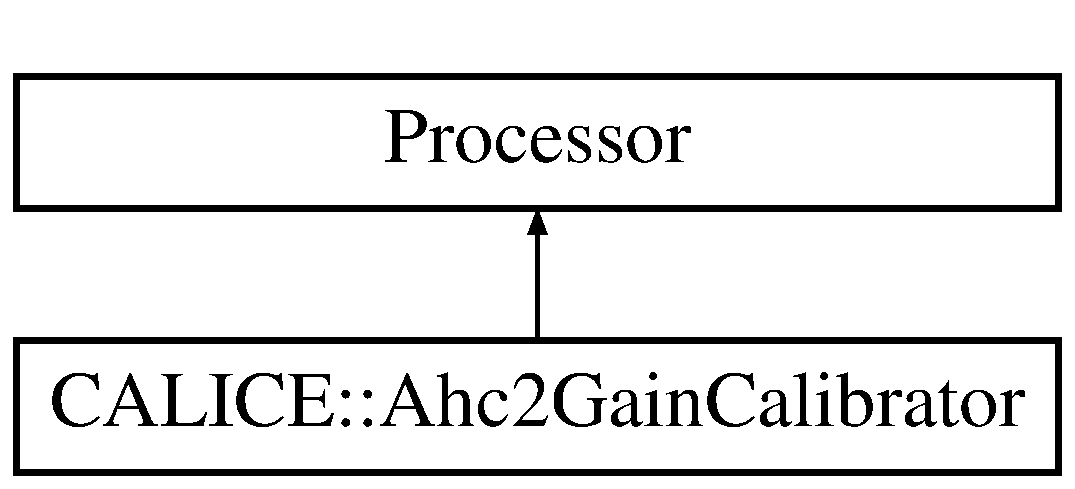
\includegraphics[height=2.000000cm]{classCALICE_1_1Ahc2GainCalibrator}
\end{center}
\end{figure}
\subsection*{Data Structures}
\begin{DoxyCompactItemize}
\item 
class {\bf Calib\-Spectrum}
\item 
class {\bf Pedestal\-Calibrator}
\end{DoxyCompactItemize}
\subsection*{Public Member Functions}
\begin{DoxyCompactItemize}
\item 
virtual Processor $\ast$ {\bfseries new\-Processor} ()\label{classCALICE_1_1Ahc2GainCalibrator_a2cd18d77eb3800a2a283d16fe29f2c6f}

\item 
{\bf Ahc2\-Gain\-Calibrator} ()\label{classCALICE_1_1Ahc2GainCalibrator_a6320419c6cfdfdc64dd7fa96cce09d9f}

\begin{DoxyCompactList}\small\item\em Default constructor. \end{DoxyCompactList}\item 
virtual void {\bf init} ()\label{classCALICE_1_1Ahc2GainCalibrator_ac1573d5b6cad18fe1f8050d2f38c3a3f}

\begin{DoxyCompactList}\small\item\em Marlin \doxyref{init()}{p.}{classCALICE_1_1Ahc2GainCalibrator_ac1573d5b6cad18fe1f8050d2f38c3a3f} function. \end{DoxyCompactList}\item 
virtual void {\bf process\-Run\-Header} (L\-C\-Event $\ast$evt)\label{classCALICE_1_1Ahc2GainCalibrator_ac34abdc73d3b0b3386897014967eac63}

\begin{DoxyCompactList}\small\item\em Marlin \doxyref{process\-Run\-Header()}{p.}{classCALICE_1_1Ahc2GainCalibrator_ac34abdc73d3b0b3386897014967eac63} function. \end{DoxyCompactList}\item 
virtual void {\bf process\-Event} (L\-C\-Event $\ast$evt)\label{classCALICE_1_1Ahc2GainCalibrator_a72d95ed3241e4d3ef4206f45a33b33b1}

\begin{DoxyCompactList}\small\item\em Marlin \doxyref{process\-Event()}{p.}{classCALICE_1_1Ahc2GainCalibrator_a72d95ed3241e4d3ef4206f45a33b33b1} function. \end{DoxyCompactList}\item 
virtual void {\bf check} (L\-C\-Event $\ast$evt)\label{classCALICE_1_1Ahc2GainCalibrator_a5c59755e3e8a923997242ec29c277f2a}

\begin{DoxyCompactList}\small\item\em Marlin \doxyref{check()}{p.}{classCALICE_1_1Ahc2GainCalibrator_a5c59755e3e8a923997242ec29c277f2a} function. \end{DoxyCompactList}\item 
virtual void {\bf end} ()\label{classCALICE_1_1Ahc2GainCalibrator_a89ae814af7ff3c7f4eb177e1c0d17bc2}

\begin{DoxyCompactList}\small\item\em Marlin \doxyref{end()}{p.}{classCALICE_1_1Ahc2GainCalibrator_a89ae814af7ff3c7f4eb177e1c0d17bc2} function. \end{DoxyCompactList}\item 
bool {\bfseries Check\-Spectrum} (T\-Spectrum $\ast$spec)\label{classCALICE_1_1Ahc2GainCalibrator_ae25b20654d17569dbfe647fd8c16aca6}

\end{DoxyCompactItemize}
\subsection*{Protected Attributes}
\begin{DoxyCompactItemize}
\item 
{\bf Pedestal\-Calibrator} $\ast$ {\bfseries pedestal}\label{classCALICE_1_1Ahc2GainCalibrator_a7bff616a9e98da157f91629b8bf7d68d}

\item 
std\-::string {\bf \-\_\-input\-Col\-Name}\label{classCALICE_1_1Ahc2GainCalibrator_a2068e292da9d8c573029df96bec5ab4a}

\begin{DoxyCompactList}\small\item\em Input L\-C\-I\-O Collection name. \end{DoxyCompactList}\item 
std\-::string {\bf \-\_\-rootfile\-Name}\label{classCALICE_1_1Ahc2GainCalibrator_a07d0bb7b6b0e619db43e06f7402a892d}

\begin{DoxyCompactList}\small\item\em Output Rootfile name. \end{DoxyCompactList}\item 
std\-::string {\bf \-\_\-gainfile\-Name}\label{classCALICE_1_1Ahc2GainCalibrator_aaa4d9833aad27df6085dd88a9046a797}

\begin{DoxyCompactList}\small\item\em Output tsv file name. \end{DoxyCompactList}\item 
std\-::string {\bf \-\_\-input\-Mem\-Offset\-Name}\label{classCALICE_1_1Ahc2GainCalibrator_a339263877a8635af1140647fad25784a}

\begin{DoxyCompactList}\small\item\em Path to the Memcell offset values. \end{DoxyCompactList}\item 
bool {\bf \-\_\-is\-H\-G\-L\-G}\label{classCALICE_1_1Ahc2GainCalibrator_a3bfa6ec3a49a85bb22d494a88f9f9bc9}

\begin{DoxyCompactList}\small\item\em Files run with A\-D\-C H\-G-\/\-L\-G? \end{DoxyCompactList}\item 
bool {\bfseries \-\_\-\-To\-Check\-Spectrum}\label{classCALICE_1_1Ahc2GainCalibrator_ab3e2e78e39abbab307a2ca82f6f5bbeb}

\item 
bool {\bfseries \-\_\-\-To\-Check\-Mean}\label{classCALICE_1_1Ahc2GainCalibrator_a5383497661cba550f7fcf7d77bac8c25}

\item 
bool {\bf \-\_\-take\-Pedestal}\label{classCALICE_1_1Ahc2GainCalibrator_a7e2981ac6c30e1e17983cc15404d0ba2}

\begin{DoxyCompactList}\small\item\em take pedestal memory cell offset \end{DoxyCompactList}\item 
std\-::string {\bf \-\_\-v\-Calib}\label{classCALICE_1_1Ahc2GainCalibrator_ab87279a2a7077d60e14234bc53cdd222}

\begin{DoxyCompactList}\small\item\em L\-E\-D calib voltage in m\-V. \end{DoxyCompactList}\item 
float {\bfseries b\-\_\-chi2}\label{classCALICE_1_1Ahc2GainCalibrator_ad7ef3b652f31a5747995f10c72d087c4}

\item 
float {\bfseries b\-\_\-chip}\label{classCALICE_1_1Ahc2GainCalibrator_a9106a894efcf5db9ac569a880b390fe4}

\item 
float {\bfseries b\-\_\-chan}\label{classCALICE_1_1Ahc2GainCalibrator_ab60e0f696626eef745dc8132c4c9fad4}

\item 
float {\bfseries b\-\_\-\-Vcalib}\label{classCALICE_1_1Ahc2GainCalibrator_ae14581654a58c27979ec8212646dcf80}

\item 
T\-File $\ast$ {\bf output\-\_\-file}\label{classCALICE_1_1Ahc2GainCalibrator_aea956c36024f81e4d698757e967758b1}

\begin{DoxyCompactList}\small\item\em Pointer to output rootfile. \end{DoxyCompactList}\item 
T\-File $\ast$ {\bfseries f\-Test}\label{classCALICE_1_1Ahc2GainCalibrator_a864a38222ab9d49b9d23b34a20467f6f}

\item 
T\-Tree $\ast$ {\bfseries t\-Test}\label{classCALICE_1_1Ahc2GainCalibrator_a4b2b85b472016465f7f84442d8a77759}

\item 
T\-File $\ast$ {\bfseries f\-High\-Signal}\label{classCALICE_1_1Ahc2GainCalibrator_a6772ce33e107f907b9525734cf4ed1f3}

\item 
T\-H1\-D $\ast$ {\bf h\-Chi\-Square}\label{classCALICE_1_1Ahc2GainCalibrator_a05fb396911d9708a9a216d6f791255f7}

\begin{DoxyCompactList}\small\item\em Pointer to histogram Chi\-Square all. \end{DoxyCompactList}\item 
T\-H1\-D $\ast$ {\bfseries h\-Fit\-Over\-F\-F\-T}\label{classCALICE_1_1Ahc2GainCalibrator_ab04684225bb64e36e4fb829b23c4f326}

\item 
T\-H2\-D $\ast$ {\bfseries h\-Fit2\-F\-F\-T}\label{classCALICE_1_1Ahc2GainCalibrator_aa43b8107e142e992d5a6176d7fe7b706}

\item 
map$<$ int, std\-::vector\\*
$<$ {\bf Calib\-Spectrum} $\ast$ $>$ $>$ {\bf histos}\label{classCALICE_1_1Ahc2GainCalibrator_a86f2bfc90b06ffeb0a0e3c3a4d933ca4}

\begin{DoxyCompactList}\small\item\em map for each chip containing 36 histograms \end{DoxyCompactList}\end{DoxyCompactItemize}


\subsection{Detailed Description}


Definition at line 61 of file Ahc2\-Gain\-Calibrator.\-hh.



The documentation for this class was generated from the following files\-:\begin{DoxyCompactItemize}
\item 
Ahc2\-Gain\-Calibrator.\-hh\item 
Ahc2\-Gain\-Calibrator.\-cc\end{DoxyCompactItemize}

\section{Ahc2\-Mip\-Track\-Finder Class Reference}
\label{classAhc2MipTrackFinder}\index{Ahc2\-Mip\-Track\-Finder@{Ahc2\-Mip\-Track\-Finder}}
Inheritance diagram for Ahc2\-Mip\-Track\-Finder\-:\begin{figure}[H]
\begin{center}
\leavevmode
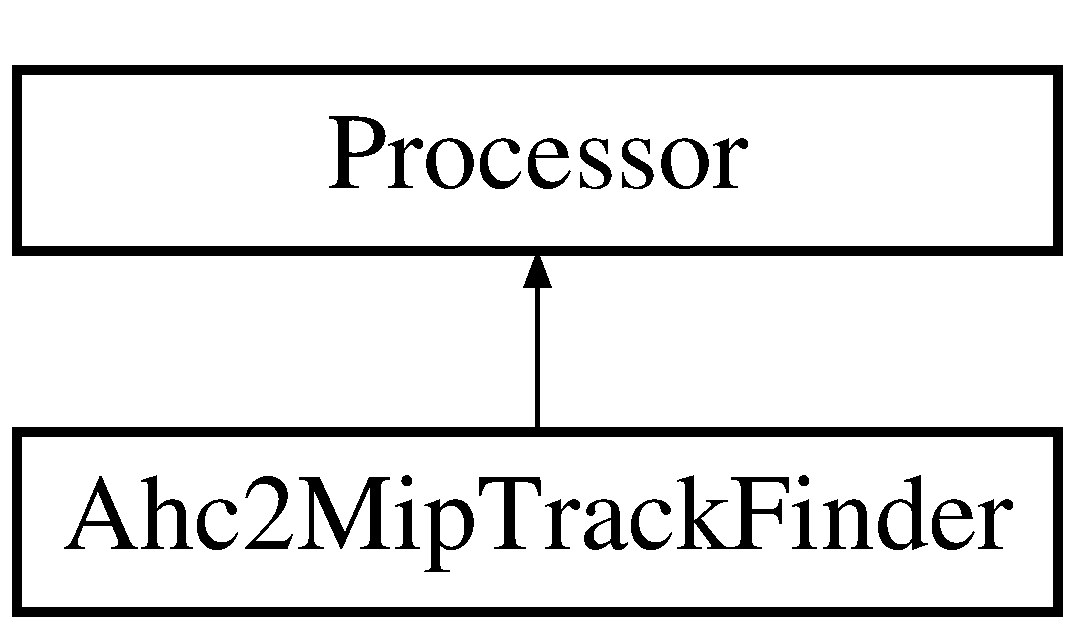
\includegraphics[height=2.000000cm]{classAhc2MipTrackFinder}
\end{center}
\end{figure}
\subsection*{Public Member Functions}
\begin{DoxyCompactItemize}
\item 
virtual Processor $\ast$ {\bfseries new\-Processor} ()\label{classAhc2MipTrackFinder_a0256c784c23379a534a1834e94d82f27}

\item 
{\bf Ahc2\-Mip\-Track\-Finder} ()\label{classAhc2MipTrackFinder_a8757b045cbc705bb82cfe8536dddf72e}

\begin{DoxyCompactList}\small\item\em Default constructor. \end{DoxyCompactList}\item 
{\bf $\sim$\-Ahc2\-Mip\-Track\-Finder} ()\label{classAhc2MipTrackFinder_adff2034892ccb8427a3d812b566fa206}

\begin{DoxyCompactList}\small\item\em Default destructor. \end{DoxyCompactList}\item 
virtual void {\bf init} ()\label{classAhc2MipTrackFinder_a00ae45fba69736e63a3c5f0a04631c94}

\begin{DoxyCompactList}\small\item\em Marlin \doxyref{init()}{p.}{classAhc2MipTrackFinder_a00ae45fba69736e63a3c5f0a04631c94} function. \end{DoxyCompactList}\item 
virtual void {\bf process\-Run\-Header} (L\-C\-Event $\ast$evt)\label{classAhc2MipTrackFinder_a31d0fabce12e738197dae9b6f0fc3df5}

\begin{DoxyCompactList}\small\item\em Marlin \doxyref{process\-Run\-Header()}{p.}{classAhc2MipTrackFinder_a31d0fabce12e738197dae9b6f0fc3df5} function. \end{DoxyCompactList}\item 
virtual void {\bf process\-Event} (L\-C\-Event $\ast$evt)\label{classAhc2MipTrackFinder_a5a25f8ca7c7a3e7e083c5bbf8bcb4c38}

\begin{DoxyCompactList}\small\item\em Marlin \doxyref{process\-Event()}{p.}{classAhc2MipTrackFinder_a5a25f8ca7c7a3e7e083c5bbf8bcb4c38} function. \end{DoxyCompactList}\item 
virtual void {\bf check} (L\-C\-Event $\ast$evt)\label{classAhc2MipTrackFinder_ac108cb9587263b9877dc80d81bc1548a}

\begin{DoxyCompactList}\small\item\em Marlin \doxyref{check()}{p.}{classAhc2MipTrackFinder_ac108cb9587263b9877dc80d81bc1548a} function. \end{DoxyCompactList}\item 
virtual void {\bf end} ()\label{classAhc2MipTrackFinder_a2967396eb150a9fc32ca4414ed6301d8}

\begin{DoxyCompactList}\small\item\em Marlin \doxyref{end()}{p.}{classAhc2MipTrackFinder_a2967396eb150a9fc32ca4414ed6301d8} function. \end{DoxyCompactList}\item 
void {\bfseries print\-Parameters} ()\label{classAhc2MipTrackFinder_a04d6877bfc8101ecece5ff28594b7445}

\item 
int {\bf Fill2\-D\-Map} (Tower\-Hit\-Vector\-H\-C\-A\-L \&Tower\-Map, int I, int J, int K, float x, float y, float z, Float\-\_\-t ahc\-\_\-hit\-Energy, Float\-\_\-t ahc\-\_\-hit\-Time, Int\-\_\-t ahc\-\_\-hit\-Type, int Cell\-I\-D0)
\begin{DoxyCompactList}\small\item\em Fill H\-C\-A\-L Towers. \end{DoxyCompactList}\item 
int {\bf Fill2\-D\-Map} (Tower\-Hit\-Vector\-E\-C\-A\-L \&Tower\-Map, int I, int J, int K, float x, float y, float z, Float\-\_\-t emc\-\_\-hit\-Energy, Float\-\_\-t emc\-\_\-hit\-Time, Int\-\_\-t emc\-\_\-hit\-Type, int Cell\-I\-D0)
\begin{DoxyCompactList}\small\item\em Fill E\-C\-A\-L Towers. \end{DoxyCompactList}\item 
int {\bf select\-Tower\-N\-Hits} (Tower\-Hit\-Vector\-H\-C\-A\-L \&towers, unsigned int Min\-N\-Hits)
\begin{DoxyCompactList}\small\item\em Select H\-C\-A\-L Towers with number of hits over Min\-N\-Hits. \end{DoxyCompactList}\item 
bool {\bf Check\-\_\-\-T0} (int Ihit, int Jhit, int Khit)
\begin{DoxyCompactList}\small\item\em Reject T0 hits. \end{DoxyCompactList}\item 
bool {\bf Check\-\_\-\-Cherenkow} (int Ihit, int Jhit, int Khit)
\begin{DoxyCompactList}\small\item\em Reject Cherenkow hits. \end{DoxyCompactList}\item 
bool {\bf Check\-Overlap} (pair$<$ float, float $>$ Coordinates\-\_\-\-E\-C\-A\-L, pair$<$ float, float $>$ Coordinates\-\_\-\-H\-C\-A\-L)
\begin{DoxyCompactList}\small\item\em Check E\-C\-A\-L Strip overlap with H\-C\-A\-L Tower. \end{DoxyCompactList}\item 
int {\bf Increment\-Overlap} (vector$<$ {\bf Ecal\-Single\-Hit} $>$ \&E\-C\-A\-L\-Hits)
\begin{DoxyCompactList}\small\item\em Increment Overlap parameter of a E\-C\-A\-L Hit. \end{DoxyCompactList}\end{DoxyCompactItemize}
\subsection*{Protected Attributes}
\begin{DoxyCompactItemize}
\item 
Tower\-Hit\-Vector\-H\-C\-A\-L {\bf \-\_\-tower\-H\-C\-A\-L\-Hits}\label{classAhc2MipTrackFinder_a5f33d06e9624290d728f2bf1a52498bf}

\begin{DoxyCompactList}\small\item\em H\-C\-A\-L Tower. \end{DoxyCompactList}\item 
Tower\-Hit\-Vector\-E\-C\-A\-L {\bf \-\_\-tower\-E\-C\-A\-L\-Hits}\label{classAhc2MipTrackFinder_abba8352972ee2b87a2fe9e773f4f28a1}

\begin{DoxyCompactList}\small\item\em E\-C\-A\-L Tower. \end{DoxyCompactList}\item 
std\-::string {\bf \-\_\-ahcinput\-Col\-Name}\label{classAhc2MipTrackFinder_af7abccb82ee7ab200473b2eb3ca88b27}

\begin{DoxyCompactList}\small\item\em H\-C\-A\-L input Collection. \end{DoxyCompactList}\item 
std\-::string {\bf \-\_\-emcinput\-Col\-Name}\label{classAhc2MipTrackFinder_add143db43629dd17b179d359d5ae3e5a}

\begin{DoxyCompactList}\small\item\em E\-C\-A\-L input Collection. \end{DoxyCompactList}\item 
std\-::string {\bf \-\_\-ahc\-Hit\-Output\-Col\-Name}\label{classAhc2MipTrackFinder_a45086d9f8c9892ee54d50e6544840763}

\begin{DoxyCompactList}\small\item\em H\-C\-A\-L output Collection. \end{DoxyCompactList}\item 
std\-::string {\bf \-\_\-emc\-Hit\-Output\-Col\-Name}\label{classAhc2MipTrackFinder_a4f55b4dc04e17168c33e349a556e8ab0}

\begin{DoxyCompactList}\small\item\em E\-C\-A\-L output Collection. \end{DoxyCompactList}\item 
std\-::string {\bfseries \-\_\-encoding\-E\-C\-A\-L}\label{classAhc2MipTrackFinder_a05ad775608ce9d70dfdae48756b36c82}

\item 
std\-::string {\bfseries \-\_\-encoding\-H\-C\-A\-L}\label{classAhc2MipTrackFinder_a75911ea13aa65e559b256b0887a523d6}

\item 
bool {\bfseries \-\_\-keep\-T0\-Cherenkow}\label{classAhc2MipTrackFinder_ab3ef40b963a91986f28dba9bcd817ccc}

\item 
int {\bf \-\_\-cut\-N\-Tower\-Hits}
\begin{DoxyCompactList}\small\item\em keep T0 and Cherenkow in output collection \end{DoxyCompactList}\item 
int {\bf \-\_\-cut\-N\-Layer\-Hits}\label{classAhc2MipTrackFinder_af8e1dad24d51f622a4b6ffc97337be09}

\begin{DoxyCompactList}\small\item\em Cut on Number of hits in a Layer. \end{DoxyCompactList}\item 
int {\bf \-\_\-n\-Max\-Hits}\label{classAhc2MipTrackFinder_a358ea560c80ae158ddef3f7f8072327c}

\begin{DoxyCompactList}\small\item\em Maximum number of hits per event. \end{DoxyCompactList}\item 
int {\bf \-\_\-n\-Min\-Hits}\label{classAhc2MipTrackFinder_a773a83d2634d654d9d3510e150c0ae56}

\begin{DoxyCompactList}\small\item\em Minimum number of hits per event. \end{DoxyCompactList}\item 
String\-Vec {\bf \-\_\-\-T0\-Vector}\label{classAhc2MipTrackFinder_a97d9f69dad58f11abf3b447e7af82a45}

\begin{DoxyCompactList}\small\item\em Vector containing T0s. \end{DoxyCompactList}\item 
String\-Vec {\bf \-\_\-\-Cherenkow\-Vector}\label{classAhc2MipTrackFinder_a546a544b370f3524820bb616dc7c779d}

\begin{DoxyCompactList}\small\item\em Vector containing Cherenkows. \end{DoxyCompactList}\item 
vector$<$ int $>$ {\bf \-\_\-map\-T0s}\label{classAhc2MipTrackFinder_a652a66e5a9cf9e6467cc7261c138c216}

\begin{DoxyCompactList}\small\item\em map for T0s \end{DoxyCompactList}\item 
vector$<$ int $>$ {\bf \-\_\-map\-Cherenkows}\label{classAhc2MipTrackFinder_a29462e353cab93b227f1ef92edb9f8d0}

\begin{DoxyCompactList}\small\item\em map for Cherenkows \end{DoxyCompactList}\item 
vector$<$ int $>$ {\bf Hit\-Perlayer}\label{classAhc2MipTrackFinder_a824c3cdd65b0b903f331d78d93ba6059}

\begin{DoxyCompactList}\small\item\em Number of hits per layer before tracking to reject late pion showers. \end{DoxyCompactList}\item 
int {\bfseries n\-H\-C\-A\-Ltracks}\label{classAhc2MipTrackFinder_aa83d1d1d65865e56991ad5f0c40e74de}

\item 
int {\bfseries \-\_\-n\-Evt}\label{classAhc2MipTrackFinder_a542724bf3cc0745407ce97e785951167}

\item 
int {\bfseries \-\_\-n\-Run}\label{classAhc2MipTrackFinder_a45930d24e5ea2dbeade5ce877de8a9f8}

\end{DoxyCompactItemize}


\subsection{Detailed Description}


Definition at line 27 of file Ahc2\-Mip\-Track\-Finder.\-hh.



\subsection{Member Function Documentation}
\index{Ahc2\-Mip\-Track\-Finder@{Ahc2\-Mip\-Track\-Finder}!Check\-\_\-\-Cherenkow@{Check\-\_\-\-Cherenkow}}
\index{Check\-\_\-\-Cherenkow@{Check\-\_\-\-Cherenkow}!Ahc2MipTrackFinder@{Ahc2\-Mip\-Track\-Finder}}
\subsubsection[{Check\-\_\-\-Cherenkow}]{\setlength{\rightskip}{0pt plus 5cm}bool Ahc2\-Mip\-Track\-Finder\-::\-Check\-\_\-\-Cherenkow (
\begin{DoxyParamCaption}
\item[{int}]{Ihit, }
\item[{int}]{Jhit, }
\item[{int}]{Khit}
\end{DoxyParamCaption}
)}\label{classAhc2MipTrackFinder_ac4fab0956d6a015ff1e1de4ec6eb4fd7}


Reject Cherenkow hits. 


\begin{DoxyParams}{Parameters}
{\em Ihit} & -\/ I coordinate of the hit \\
\hline
{\em Jhit} & -\/ J coordinate of the hit \\
\hline
{\em Khit} & -\/ K coordinate of the hit \\
\hline
\end{DoxyParams}
\begin{DoxyReturn}{Returns}
-\/ true if Cherenkow Hit otherwise false 
\end{DoxyReturn}


Definition at line 662 of file Ahc2\-Mip\-Track\-Finder.\-cc.



References \-\_\-map\-Cherenkows.



Referenced by process\-Event().

\index{Ahc2\-Mip\-Track\-Finder@{Ahc2\-Mip\-Track\-Finder}!Check\-\_\-\-T0@{Check\-\_\-\-T0}}
\index{Check\-\_\-\-T0@{Check\-\_\-\-T0}!Ahc2MipTrackFinder@{Ahc2\-Mip\-Track\-Finder}}
\subsubsection[{Check\-\_\-\-T0}]{\setlength{\rightskip}{0pt plus 5cm}bool Ahc2\-Mip\-Track\-Finder\-::\-Check\-\_\-\-T0 (
\begin{DoxyParamCaption}
\item[{int}]{Ihit, }
\item[{int}]{Jhit, }
\item[{int}]{Khit}
\end{DoxyParamCaption}
)}\label{classAhc2MipTrackFinder_a8b95ddc6aaa65392ae2acab94ae1871f}


Reject T0 hits. 


\begin{DoxyParams}{Parameters}
{\em Ihit} & -\/ I coordinate of the hit \\
\hline
{\em Jhit} & -\/ J coordinate of the hit \\
\hline
{\em Khit} & -\/ K coordinate of the hit \\
\hline
\end{DoxyParams}
\begin{DoxyReturn}{Returns}
-\/ true if T0 Hit otherwise false 
\end{DoxyReturn}


Definition at line 640 of file Ahc2\-Mip\-Track\-Finder.\-cc.



References \-\_\-map\-T0s.



Referenced by process\-Event().

\index{Ahc2\-Mip\-Track\-Finder@{Ahc2\-Mip\-Track\-Finder}!Check\-Overlap@{Check\-Overlap}}
\index{Check\-Overlap@{Check\-Overlap}!Ahc2MipTrackFinder@{Ahc2\-Mip\-Track\-Finder}}
\subsubsection[{Check\-Overlap}]{\setlength{\rightskip}{0pt plus 5cm}bool Ahc2\-Mip\-Track\-Finder\-::\-Check\-Overlap (
\begin{DoxyParamCaption}
\item[{pair$<$ float, float $>$}]{Coordinates\-\_\-\-E\-C\-A\-L, }
\item[{pair$<$ float, float $>$}]{Coordinates\-\_\-\-H\-C\-A\-L}
\end{DoxyParamCaption}
)}\label{classAhc2MipTrackFinder_a52af0355bb75e7f7b096c2809b1be24f}


Check E\-C\-A\-L Strip overlap with H\-C\-A\-L Tower. 


\begin{DoxyParams}{Parameters}
{\em Coordinates\-\_\-\-E\-C\-A\-L} & -\/ x,y coordinates of the E\-C\-A\-L hit \\
\hline
{\em Coordinates\-\_\-\-H\-C\-A\-L} & -\/ x,y coordinates of the H\-C\-A\-L hit \\
\hline
\end{DoxyParams}
\begin{DoxyReturn}{Returns}
-\/ true if overlap otherwise false 
\end{DoxyReturn}


Definition at line 621 of file Ahc2\-Mip\-Track\-Finder.\-cc.

\index{Ahc2\-Mip\-Track\-Finder@{Ahc2\-Mip\-Track\-Finder}!Fill2\-D\-Map@{Fill2\-D\-Map}}
\index{Fill2\-D\-Map@{Fill2\-D\-Map}!Ahc2MipTrackFinder@{Ahc2\-Mip\-Track\-Finder}}
\subsubsection[{Fill2\-D\-Map}]{\setlength{\rightskip}{0pt plus 5cm}int Ahc2\-Mip\-Track\-Finder\-::\-Fill2\-D\-Map (
\begin{DoxyParamCaption}
\item[{Tower\-Hit\-Vector\-H\-C\-A\-L \&}]{Tower\-Map, }
\item[{int}]{I, }
\item[{int}]{J, }
\item[{int}]{K, }
\item[{float}]{x, }
\item[{float}]{y, }
\item[{float}]{z, }
\item[{Float\-\_\-t}]{ahc\-\_\-hit\-Energy, }
\item[{Float\-\_\-t}]{ahc\-\_\-hit\-Time, }
\item[{Int\-\_\-t}]{ahc\-\_\-hit\-Type, }
\item[{int}]{Cell\-I\-D0}
\end{DoxyParamCaption}
)}\label{classAhc2MipTrackFinder_aa87ebbfea543c6d8631ff274b480acd9}


Fill H\-C\-A\-L Towers. 


\begin{DoxyParams}{Parameters}
{\em Tower\-Map} & -\/ H\-C\-A\-L Tower\-Map \\
\hline
{\em I} & -\/ I coordinate of the hit \\
\hline
{\em J} & -\/ J coordinate of the hit \\
\hline
{\em K} & -\/ K coordinate of the hit \\
\hline
{\em x} & -\/ x coordinate of the hit \\
\hline
{\em y} & -\/ y coordinate of the hit \\
\hline
{\em z} & -\/ z coordinate of the hit \\
\hline
{\em ahc\-\_\-hit\-Energy} & -\/ Energy of the hit \\
\hline
{\em ahc\-\_\-hit\-Time} & -\/ Time of the hit \\
\hline
{\em ahc\-\_\-hit\-Type} & -\/ Type of the hit \\
\hline
{\em Cell\-I\-D0} & -\/ Cell\-I\-D of the hit \\
\hline
\end{DoxyParams}


Definition at line 510 of file Ahc2\-Mip\-Track\-Finder.\-cc.



Referenced by process\-Event().

\index{Ahc2\-Mip\-Track\-Finder@{Ahc2\-Mip\-Track\-Finder}!Fill2\-D\-Map@{Fill2\-D\-Map}}
\index{Fill2\-D\-Map@{Fill2\-D\-Map}!Ahc2MipTrackFinder@{Ahc2\-Mip\-Track\-Finder}}
\subsubsection[{Fill2\-D\-Map}]{\setlength{\rightskip}{0pt plus 5cm}int Ahc2\-Mip\-Track\-Finder\-::\-Fill2\-D\-Map (
\begin{DoxyParamCaption}
\item[{Tower\-Hit\-Vector\-E\-C\-A\-L \&}]{Tower\-Map, }
\item[{int}]{I, }
\item[{int}]{J, }
\item[{int}]{K, }
\item[{float}]{x, }
\item[{float}]{y, }
\item[{float}]{z, }
\item[{Float\-\_\-t}]{emc\-\_\-hit\-Energy, }
\item[{Float\-\_\-t}]{emc\-\_\-hit\-Time, }
\item[{Int\-\_\-t}]{emc\-\_\-hit\-Type, }
\item[{int}]{Cell\-I\-D0}
\end{DoxyParamCaption}
)}\label{classAhc2MipTrackFinder_a4133250e906d292eb5e63c6796d0204f}


Fill E\-C\-A\-L Towers. 


\begin{DoxyParams}{Parameters}
{\em Tower\-Map} & -\/ E\-C\-A\-L Tower\-Map \\
\hline
{\em I} & -\/ I coordinate of the hit \\
\hline
{\em J} & -\/ J coordinate of the hit \\
\hline
{\em K} & -\/ K coordinate of the hit \\
\hline
{\em x} & -\/ x coordinate of the hit \\
\hline
{\em y} & -\/ y coordinate of the hit \\
\hline
{\em z} & -\/ z coordinate of the hit \\
\hline
{\em emc\-\_\-hit\-Energy} & -\/ Energy of the hit \\
\hline
{\em emc\-\_\-hit\-Time} & -\/ Time of the hit \\
\hline
{\em emc\-\_\-hit\-Type} & -\/ Type of the hit \\
\hline
{\em Cell\-I\-D0} & -\/ Cell\-I\-D of the hit \\
\hline
\end{DoxyParams}


Definition at line 537 of file Ahc2\-Mip\-Track\-Finder.\-cc.

\index{Ahc2\-Mip\-Track\-Finder@{Ahc2\-Mip\-Track\-Finder}!Increment\-Overlap@{Increment\-Overlap}}
\index{Increment\-Overlap@{Increment\-Overlap}!Ahc2MipTrackFinder@{Ahc2\-Mip\-Track\-Finder}}
\subsubsection[{Increment\-Overlap}]{\setlength{\rightskip}{0pt plus 5cm}int Ahc2\-Mip\-Track\-Finder\-::\-Increment\-Overlap (
\begin{DoxyParamCaption}
\item[{vector$<$ {\bf Ecal\-Single\-Hit} $>$ \&}]{E\-C\-A\-L\-Hits}
\end{DoxyParamCaption}
)}\label{classAhc2MipTrackFinder_afe6b54cb68bc697386b875696d75a97d}


Increment Overlap parameter of a E\-C\-A\-L Hit. 


\begin{DoxyParams}{Parameters}
{\em E\-C\-A\-L\-Hits} & -\/ vector containing E\-C\-A\-L hits \\
\hline
\end{DoxyParams}


Definition at line 604 of file Ahc2\-Mip\-Track\-Finder.\-cc.

\index{Ahc2\-Mip\-Track\-Finder@{Ahc2\-Mip\-Track\-Finder}!select\-Tower\-N\-Hits@{select\-Tower\-N\-Hits}}
\index{select\-Tower\-N\-Hits@{select\-Tower\-N\-Hits}!Ahc2MipTrackFinder@{Ahc2\-Mip\-Track\-Finder}}
\subsubsection[{select\-Tower\-N\-Hits}]{\setlength{\rightskip}{0pt plus 5cm}int Ahc2\-Mip\-Track\-Finder\-::select\-Tower\-N\-Hits (
\begin{DoxyParamCaption}
\item[{Tower\-Hit\-Vector\-H\-C\-A\-L \&}]{towers, }
\item[{unsigned int}]{Min\-N\-Hits}
\end{DoxyParamCaption}
)}\label{classAhc2MipTrackFinder_a09ca0edbf3c8911ccf76167d1e8048ee}


Select H\-C\-A\-L Towers with number of hits over Min\-N\-Hits. 


\begin{DoxyParams}{Parameters}
{\em towers} & -\/ H\-C\-A\-L Towers \\
\hline
{\em Min\-N\-Hits} & -\/ Minimum on Number of hits in a Tower \\
\hline
\end{DoxyParams}
\begin{DoxyReturn}{Returns}
-\/ Number of Towers left 
\end{DoxyReturn}


Definition at line 566 of file Ahc2\-Mip\-Track\-Finder.\-cc.



Referenced by process\-Event().



\subsection{Field Documentation}
\index{Ahc2\-Mip\-Track\-Finder@{Ahc2\-Mip\-Track\-Finder}!\-\_\-cut\-N\-Tower\-Hits@{\-\_\-cut\-N\-Tower\-Hits}}
\index{\-\_\-cut\-N\-Tower\-Hits@{\-\_\-cut\-N\-Tower\-Hits}!Ahc2MipTrackFinder@{Ahc2\-Mip\-Track\-Finder}}
\subsubsection[{\-\_\-cut\-N\-Tower\-Hits}]{\setlength{\rightskip}{0pt plus 5cm}int Ahc2\-Mip\-Track\-Finder\-::\-\_\-cut\-N\-Tower\-Hits\hspace{0.3cm}{\ttfamily [protected]}}\label{classAhc2MipTrackFinder_ac4a5ee1f4675658f8136ee1f5b1a1c2e}


keep T0 and Cherenkow in output collection 

Cut on Number of hits in a Tower 

Definition at line 142 of file Ahc2\-Mip\-Track\-Finder.\-hh.



Referenced by Ahc2\-Mip\-Track\-Finder(), and process\-Event().



The documentation for this class was generated from the following files\-:\begin{DoxyCompactItemize}
\item 
Ahc2\-Mip\-Track\-Finder.\-hh\item 
Ahc2\-Mip\-Track\-Finder.\-cc\end{DoxyCompactItemize}

\section{C\-A\-L\-I\-C\-E\-:\-:Ahc2\-Occupancy\-Calibrator Class Reference}
\label{classCALICE_1_1Ahc2OccupancyCalibrator}\index{C\-A\-L\-I\-C\-E\-::\-Ahc2\-Occupancy\-Calibrator@{C\-A\-L\-I\-C\-E\-::\-Ahc2\-Occupancy\-Calibrator}}
Inheritance diagram for C\-A\-L\-I\-C\-E\-:\-:Ahc2\-Occupancy\-Calibrator\-:\begin{figure}[H]
\begin{center}
\leavevmode
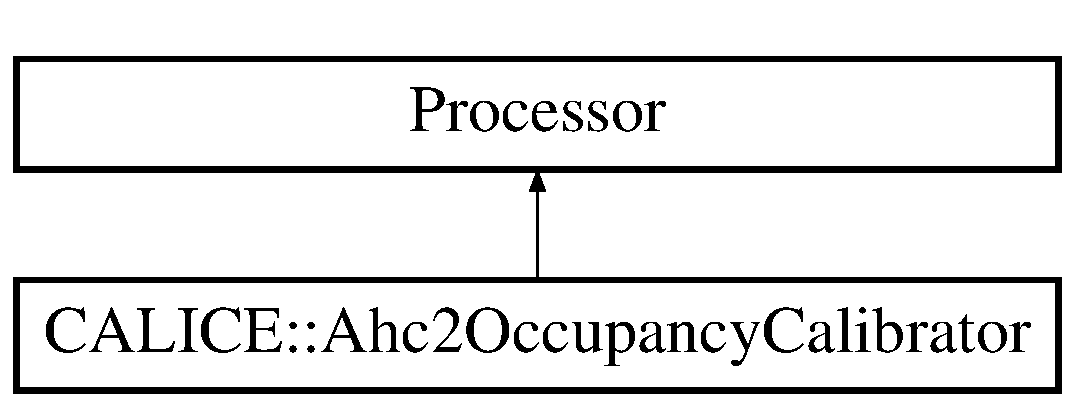
\includegraphics[height=2.000000cm]{classCALICE_1_1Ahc2OccupancyCalibrator}
\end{center}
\end{figure}
\subsection*{Data Structures}
\begin{DoxyCompactItemize}
\item 
struct {\bf Calib\-Value}
\end{DoxyCompactItemize}
\subsection*{Public Member Functions}
\begin{DoxyCompactItemize}
\item 
{\bf Ahc2\-Occupancy\-Calibrator} $\ast$ {\bfseries new\-Processor} ()\label{classCALICE_1_1Ahc2OccupancyCalibrator_ab850d8d70dc40faec36a35bb92f1b7d4}

\item 
virtual void {\bfseries init} ()\label{classCALICE_1_1Ahc2OccupancyCalibrator_ac7f750b9e258f3ad92a09ad64a94827b}

\item 
virtual void {\bfseries process\-Event} (L\-C\-Event $\ast$evt)\label{classCALICE_1_1Ahc2OccupancyCalibrator_a6c72b27a0e96d8ecc564fdcbd4b8f272}

\item 
virtual void {\bfseries end} ()\label{classCALICE_1_1Ahc2OccupancyCalibrator_a6b5ac3a8f00949655788e5677775807a}

\end{DoxyCompactItemize}
\subsection*{Protected Member Functions}
\begin{DoxyCompactItemize}
\item 
void {\bfseries Fill\-Container} (L\-C\-Event $\ast$evt)\label{classCALICE_1_1Ahc2OccupancyCalibrator_aab17d7ea8610d706f1a4110a3b4720c0}

\item 
void {\bfseries Process\-Hit} (Calorimeter\-Hit $\ast$hit, int evt\-Bx\-I\-D)\label{classCALICE_1_1Ahc2OccupancyCalibrator_a08d8f75993a010a51e479ef6b1169ec7}

\item 
void {\bfseries Fit\-Occupancy} ()\label{classCALICE_1_1Ahc2OccupancyCalibrator_ab38c7f3009dcb59ec68358f2683e60a5}

\item 
void {\bfseries Write\-Constants} ()\label{classCALICE_1_1Ahc2OccupancyCalibrator_ab68258017b327ea743a09b76a7950521}

\end{DoxyCompactItemize}
\subsection*{Protected Attributes}
\begin{DoxyCompactItemize}
\item 
std\-::map$<$ int, std\-::map$<$ int, \\*
int $>$ $>$ {\bfseries \-\_\-occupancy\-Per\-Chip}\label{classCALICE_1_1Ahc2OccupancyCalibrator_a98fd37f253000919187fda7e0e1bfc91}

\item 
std\-::map$<$ int, std\-::map$<$ int, \\*
std\-::map$<$ int, std\-::map$<$ int, \\*
std\-::map$<$ int, std\-::map$<$ int, \\*
std\-::vector$<$ float $>$ $>$ $>$ $>$ $>$ $>$ $>$ {\bfseries \-\_\-sorted\-Hit\-Container}\label{classCALICE_1_1Ahc2OccupancyCalibrator_aa0007fc4dd8929013e30b6c17016eadd}

\item 
std\-::map$<$ int, std\-::map$<$ int, \\*
std\-::map$<$ int, std\-::map$<$ int, \\*
std\-::map$<$ int, {\bf Calib\-Value} $>$ $>$ $>$ $>$ $>$ {\bfseries \-\_\-m\-\_\-calibration\-\_\-constants}\label{classCALICE_1_1Ahc2OccupancyCalibrator_a80f0878a73713a22cb155cf976fe6b8b}

\item 
int {\bfseries \-\_\-n\-Channels}\label{classCALICE_1_1Ahc2OccupancyCalibrator_ab169b46b25955ef59442dc4b97a02366}

\item 
double {\bfseries \-\_\-tdc\-Error}\label{classCALICE_1_1Ahc2OccupancyCalibrator_a01e2a7ec01c030dcb734c71b56a1b75b}

\item 
double {\bfseries \-\_\-time\-Reference\-Error}\label{classCALICE_1_1Ahc2OccupancyCalibrator_a6f963856dff73e179c4d887798385d96}

\item 
std\-::string {\bf \-\_\-hit\-In\-Col\-Name}\label{classCALICE_1_1Ahc2OccupancyCalibrator_a7d75d3932599645dc6658795cc952deb}

\begin{DoxyCompactList}\small\item\em name of the input collection \end{DoxyCompactList}\item 
std\-::string {\bfseries \-\_\-occupancy\-In\-Col\-Name}\label{classCALICE_1_1Ahc2OccupancyCalibrator_a103e15d01b57c0f782e504b25eacd20f}

\item 
std\-::string {\bf \-\_\-ahc\-Hit\-Output\-Col\-Name}\label{classCALICE_1_1Ahc2OccupancyCalibrator_aa8fd9dbe672add06d67ab9d02c091738}

\begin{DoxyCompactList}\small\item\em name of the output A\-H\-C hit collection \end{DoxyCompactList}\item 
std\-::string {\bf \-\_\-mapping\-Processor\-Name}\label{classCALICE_1_1Ahc2OccupancyCalibrator_a36e578634b06a3bbfc1d1062b9e6c5ba}

\begin{DoxyCompactList}\small\item\em name of the processor which provides the mapping \end{DoxyCompactList}\item 
std\-::string {\bfseries \-\_\-\-Ahc2\-Hardware\-Connection\-Name}\label{classCALICE_1_1Ahc2OccupancyCalibrator_a653a9a2efd9f6b5d7c50afe550561870}

\item 
std\-::string {\bf \-\_\-temperature\-Processor\-Name}\label{classCALICE_1_1Ahc2OccupancyCalibrator_ad36670eaac520cd472476bfd0f3af00f}

\begin{DoxyCompactList}\small\item\em name of the processor which provides the Si\-P\-M temperature \end{DoxyCompactList}\item 
std\-::string {\bf \-\_\-bif\-Col\-Name}\label{classCALICE_1_1Ahc2OccupancyCalibrator_a346e6ef475334068a4400c80bf9daaef}

\begin{DoxyCompactList}\small\item\em name of the processor which provides the Si\-P\-M temperature \end{DoxyCompactList}\item 
int {\bfseries \-\_\-\-B\-I\-F\-Trigger\-Input\-Source}\label{classCALICE_1_1Ahc2OccupancyCalibrator_aad631504dc281bdd1e963ed0c324e260}

\item 
std\-::string {\bfseries \-\_\-prefix}\label{classCALICE_1_1Ahc2OccupancyCalibrator_ad82f4c256b53cd8a2990027afc57497a}

\item 
bool {\bfseries \-\_\-skip\-First\-Memory\-Cell}\label{classCALICE_1_1Ahc2OccupancyCalibrator_acff5130980088ebcee6c387a62dec589}

\item 
int {\bfseries \-\_\-max\-Occupancy}\label{classCALICE_1_1Ahc2OccupancyCalibrator_ae0c86199c81c6cfe7e2ba8fa40de9e7b}

\item 
int {\bfseries \-\_\-min\-Hits\-Fit}\label{classCALICE_1_1Ahc2OccupancyCalibrator_a3988bb71c15879d20f492ee7d1de8a58}

\item 
int {\bfseries \-\_\-max\-Hits\-Fit}\label{classCALICE_1_1Ahc2OccupancyCalibrator_a9c9b2e0ac821a14845b208246f406283}

\item 
std\-::string {\bf \-\_\-cell\-Description\-Processor\-Name}\label{classCALICE_1_1Ahc2OccupancyCalibrator_a01731f039efcc81e00e184f96a98e790}

\begin{DoxyCompactList}\small\item\em name of the processor which provides the cells description \end{DoxyCompactList}\item 
Mapped\-Container\\*
$<$ Cell\-Description $>$ $\ast$ {\bf \-\_\-cell\-Descriptions}\label{classCALICE_1_1Ahc2OccupancyCalibrator_af83028233eb862a8973e23fe6f46be0f}

\begin{DoxyCompactList}\small\item\em mapped container of cells description \end{DoxyCompactList}\item 
const Ahc2\-Mapper $\ast$ {\bf \-\_\-mapper}\label{classCALICE_1_1Ahc2OccupancyCalibrator_ac9b4e7c9103d8d99a3b65b9fcf19aec9}

\begin{DoxyCompactList}\small\item\em the mapper \end{DoxyCompactList}\item 
Mapped\-Container$<$ Simple\-Value $>$ $\ast$ {\bf \-\_\-temperature\-Container}\label{classCALICE_1_1Ahc2OccupancyCalibrator_ab55012d14a3510fa4b89ae1fae372dd7}

\begin{DoxyCompactList}\small\item\em mapped container of cells temperature \end{DoxyCompactList}\item 
bool {\bf \-\_\-newdataformat}\label{classCALICE_1_1Ahc2OccupancyCalibrator_adaa51b1a6af59df6c4e1a762cb4ab722}

\begin{DoxyCompactList}\small\item\em flag for the new data format in E\-U\-D\-A\-Q \end{DoxyCompactList}\item 
bool {\bf \-\_\-is\-First\-Event}
\begin{DoxyCompactList}\small\item\em flag to switch to D\-A\-T\-A/\-M\-C at the first event, the following events should be the same. \end{DoxyCompactList}\item 
Mapped\-Container\\*
$<$ Calorimeter\-Hit\-Impl $>$ $\ast$ {\bf \-\_\-\-Hit\-Container}\label{classCALICE_1_1Ahc2OccupancyCalibrator_a75f803b0e387a026e6394d1629f53442}

\begin{DoxyCompactList}\small\item\em mapped container of A\-H\-C\-A\-L cells \end{DoxyCompactList}\item 
std\-::map$<$ int, std\-::pair$<$ int, \\*
int $>$ $>$ {\bf \-\_\-\-Hardware\-Connnection\-Container}\label{classCALICE_1_1Ahc2OccupancyCalibrator_a59ac6fbccb3f906f284a1072e744ebc0}

\begin{DoxyCompactList}\small\item\em map containing relationship between Chip\-I\-D and Module/\-Chip\-Nb \end{DoxyCompactList}\item 
int {\bfseries \-\_\-i\-Evt} = 0\label{classCALICE_1_1Ahc2OccupancyCalibrator_a1e3aaa9c9d7c8a34191f3d7fe6dc80e0}

\end{DoxyCompactItemize}


\subsection{Detailed Description}


Definition at line 29 of file Ahc2\-Occupancy\-Calibrator.\-hh.



\subsection{Field Documentation}
\index{C\-A\-L\-I\-C\-E\-::\-Ahc2\-Occupancy\-Calibrator@{C\-A\-L\-I\-C\-E\-::\-Ahc2\-Occupancy\-Calibrator}!\-\_\-is\-First\-Event@{\-\_\-is\-First\-Event}}
\index{\-\_\-is\-First\-Event@{\-\_\-is\-First\-Event}!CALICE::Ahc2OccupancyCalibrator@{C\-A\-L\-I\-C\-E\-::\-Ahc2\-Occupancy\-Calibrator}}
\subsubsection[{\-\_\-is\-First\-Event}]{\setlength{\rightskip}{0pt plus 5cm}bool C\-A\-L\-I\-C\-E\-::\-Ahc2\-Occupancy\-Calibrator\-::\-\_\-is\-First\-Event\hspace{0.3cm}{\ttfamily [protected]}}\label{classCALICE_1_1Ahc2OccupancyCalibrator_a7f980b83820cdf653a0f9028c230f2d1}


flag to switch to D\-A\-T\-A/\-M\-C at the first event, the following events should be the same. 



Definition at line 128 of file Ahc2\-Occupancy\-Calibrator.\-hh.



The documentation for this class was generated from the following files\-:\begin{DoxyCompactItemize}
\item 
Ahc2\-Occupancy\-Calibrator.\-hh\item 
Ahc2\-Occupancy\-Calibrator.\-cc\end{DoxyCompactItemize}

\section{C\-A\-L\-I\-C\-E\-:\-:Ahc2\-Offset\-Calibrator Class Reference}
\label{classCALICE_1_1Ahc2OffsetCalibrator}\index{C\-A\-L\-I\-C\-E\-::\-Ahc2\-Offset\-Calibrator@{C\-A\-L\-I\-C\-E\-::\-Ahc2\-Offset\-Calibrator}}


Processor to read S\-L\-C\-I\-O E\-U\-D\-A\-Q files and sort them according to the B\-X\-I\-D Then do the A\-H\-C\-A\-L-\/\-B\-I\-F Offset calibration by counting the number of correlated events (either a separation between E\-C\-A\-L and A\-H\-C\-A\-L collections is done by E\-U\-D\-A\-Q)  




{\ttfamily \#include $<$Ahc2\-Offset\-Calibrator.\-hh$>$}

Inheritance diagram for C\-A\-L\-I\-C\-E\-:\-:Ahc2\-Offset\-Calibrator\-:\begin{figure}[H]
\begin{center}
\leavevmode
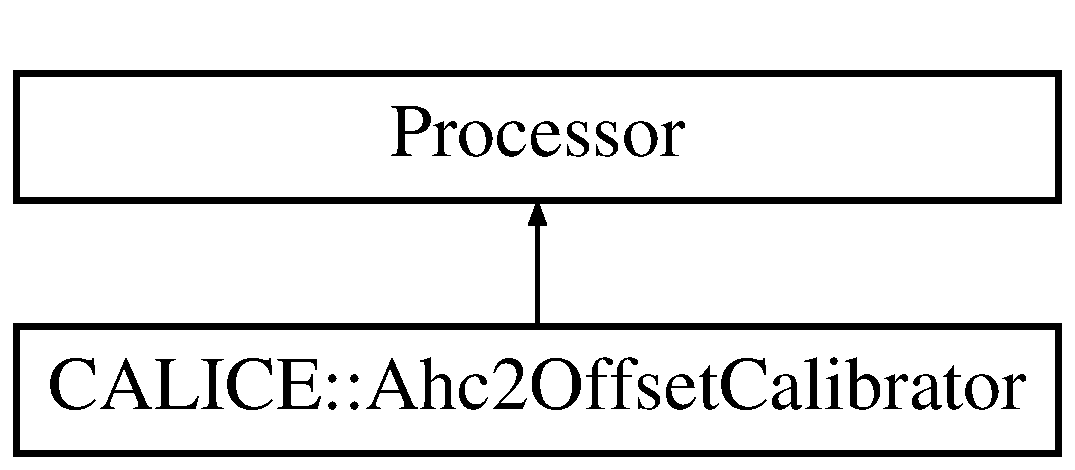
\includegraphics[height=2.000000cm]{classCALICE_1_1Ahc2OffsetCalibrator}
\end{center}
\end{figure}
\subsection*{Data Structures}
\begin{DoxyCompactItemize}
\item 
struct {\bf raw\-Data2016}
\begin{DoxyCompactList}\small\item\em The slcio data format. \end{DoxyCompactList}\end{DoxyCompactItemize}
\subsection*{Public Member Functions}
\begin{DoxyCompactItemize}
\item 
virtual Processor $\ast$ {\bf new\-Processor} ()\label{classCALICE_1_1Ahc2OffsetCalibrator_a05df86500d0a3e88f392c8ffd4f47c5d}

\begin{DoxyCompactList}\small\item\em Implementation of new Processor returns pointer to processor. \end{DoxyCompactList}\item 
void {\bf process\-Event} (L\-C\-Event $\ast$evt)\label{classCALICE_1_1Ahc2OffsetCalibrator_a2da4ab41332e8d20d11a19e71ba720e3}

\begin{DoxyCompactList}\small\item\em Creates events with L\-C\-Genreal\-Object collections from the E\-U\-D\-A\-Q input file and calls all active processors' \doxyref{process\-Event()}{p.}{classCALICE_1_1Ahc2OffsetCalibrator_a2da4ab41332e8d20d11a19e71ba720e3} and process\-Run\-Header Method. \end{DoxyCompactList}\item 
virtual void {\bf init} ()\label{classCALICE_1_1Ahc2OffsetCalibrator_ab5f576d21163aedec905e30f1b5dc9ed}

\begin{DoxyCompactList}\small\item\em init method \end{DoxyCompactList}\item 
virtual void {\bf end} ()\label{classCALICE_1_1Ahc2OffsetCalibrator_ae914d839779fc5f1aedb4c38b498d725}

\begin{DoxyCompactList}\small\item\em end method \end{DoxyCompactList}\item 
void {\bf print\-Parameters} ()\label{classCALICE_1_1Ahc2OffsetCalibrator_a62ec150e1ea85dfdf154e297091aaa6a}

\begin{DoxyCompactList}\small\item\em print parameters \end{DoxyCompactList}\end{DoxyCompactItemize}
\subsection*{Protected Attributes}
\begin{DoxyCompactItemize}
\item 
std\-::string {\bfseries \-\_\-input\-Col\-Name}\label{classCALICE_1_1Ahc2OffsetCalibrator_ab631186d636a5a8cc89d7826430d6001}

\item 
std\-::string {\bfseries \-\_\-input\-Col\-Name\-B\-I\-F}\label{classCALICE_1_1Ahc2OffsetCalibrator_a727da1f72b82aa444631738742350443}

\item 
std\-::string {\bfseries \-\_\-outputfile}\label{classCALICE_1_1Ahc2OffsetCalibrator_abf2bdf8aaff1546fbf44e780489fcd0f}

\item 
String\-Vec {\bfseries \-\_\-\-Bif\-Vector}\label{classCALICE_1_1Ahc2OffsetCalibrator_af7a865753499d7bcd9f2cff80c9abc14}

\item 
int {\bf \-\_\-run\-Number}\label{classCALICE_1_1Ahc2OffsetCalibrator_a953f31c54f24bd63fc5d90379a547bfe}

\begin{DoxyCompactList}\small\item\em The run number. \end{DoxyCompactList}\end{DoxyCompactItemize}
\subsection*{Private Attributes}
\begin{DoxyCompactItemize}
\item 
int {\bfseries Lcio\-Event\-Nr}\label{classCALICE_1_1Ahc2OffsetCalibrator_a8f4ec9a5d5bddd42972d929d53d4d66a}

\item 
std\-::map$<$ int, int $>$ {\bfseries n\-Correlated\-Evt}\label{classCALICE_1_1Ahc2OffsetCalibrator_a86f7a686af1078291cb6ddbe0849489d}

\item 
int {\bfseries Start\-Scan}\label{classCALICE_1_1Ahc2OffsetCalibrator_a4cb5c1b92c9d0ec5ef3ab2ebec6ee766}

\item 
int {\bfseries Stop\-Scan}\label{classCALICE_1_1Ahc2OffsetCalibrator_a6e49a6e97bfc13b34253a8eca9fb82da}

\item 
int {\bfseries Step\-Scan}\label{classCALICE_1_1Ahc2OffsetCalibrator_a7d99f8a22fa5f6a9f1f8b3565f216a21}

\end{DoxyCompactItemize}


\subsection{Detailed Description}
Processor to read S\-L\-C\-I\-O E\-U\-D\-A\-Q files and sort them according to the B\-X\-I\-D Then do the A\-H\-C\-A\-L-\/\-B\-I\-F Offset calibration by counting the number of correlated events (either a separation between E\-C\-A\-L and A\-H\-C\-A\-L collections is done by E\-U\-D\-A\-Q) 

\begin{DoxyAuthor}{Author}
E. Brianne, D\-E\-S\-Y Hamburg 
\end{DoxyAuthor}
\begin{DoxyDate}{Date}
May 2016 Created for 2016 testbeams E\-U\-D\-A\-Q data format and A\-H\-C\-A\-L-\/\-B\-I\-F Offset calibration. 
\end{DoxyDate}


Definition at line 23 of file Ahc2\-Offset\-Calibrator.\-hh.



The documentation for this class was generated from the following files\-:\begin{DoxyCompactItemize}
\item 
Ahc2\-Offset\-Calibrator.\-hh\item 
Ahc2\-Offset\-Calibrator.\-cc\end{DoxyCompactItemize}

\section{C\-A\-L\-I\-C\-E\-:\-:Ahc2\-Pedestal\-Calibrator Class Reference}
\label{classCALICE_1_1Ahc2PedestalCalibrator}\index{C\-A\-L\-I\-C\-E\-::\-Ahc2\-Pedestal\-Calibrator@{C\-A\-L\-I\-C\-E\-::\-Ahc2\-Pedestal\-Calibrator}}
Inheritance diagram for C\-A\-L\-I\-C\-E\-:\-:Ahc2\-Pedestal\-Calibrator\-:\begin{figure}[H]
\begin{center}
\leavevmode
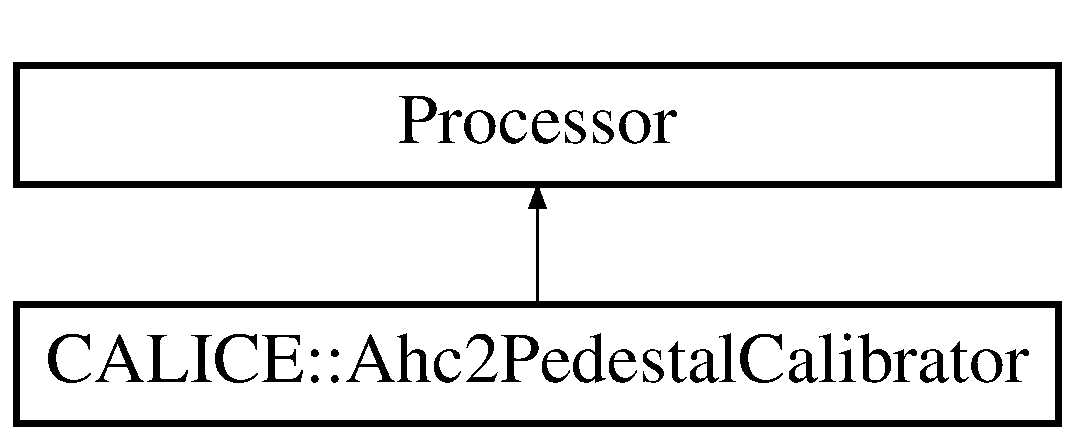
\includegraphics[height=2.000000cm]{classCALICE_1_1Ahc2PedestalCalibrator}
\end{center}
\end{figure}
\subsection*{Data Structures}
\begin{DoxyCompactItemize}
\item 
class {\bf Pedestal\-Spectrum}
\end{DoxyCompactItemize}
\subsection*{Public Member Functions}
\begin{DoxyCompactItemize}
\item 
virtual Processor $\ast$ {\bfseries new\-Processor} ()\label{classCALICE_1_1Ahc2PedestalCalibrator_a1ce8a9c8f4d41fe4541b14431f650404}

\item 
{\bf Ahc2\-Pedestal\-Calibrator} ()\label{classCALICE_1_1Ahc2PedestalCalibrator_ac998d991ba6f20e6b7ab2b2300c095a1}

\begin{DoxyCompactList}\small\item\em Default constructor. \end{DoxyCompactList}\item 
virtual void {\bf init} ()\label{classCALICE_1_1Ahc2PedestalCalibrator_a13958665050efabdee1e3a04552a9dfa}

\begin{DoxyCompactList}\small\item\em Marlin \doxyref{init()}{p.}{classCALICE_1_1Ahc2PedestalCalibrator_a13958665050efabdee1e3a04552a9dfa} function. \end{DoxyCompactList}\item 
virtual void {\bf process\-Run\-Header} (L\-C\-Event $\ast$evt)\label{classCALICE_1_1Ahc2PedestalCalibrator_aeb3418d915703b18d105f499c786f600}

\begin{DoxyCompactList}\small\item\em Marlin \doxyref{process\-Run\-Header()}{p.}{classCALICE_1_1Ahc2PedestalCalibrator_aeb3418d915703b18d105f499c786f600} function. \end{DoxyCompactList}\item 
virtual void {\bf process\-Event} (L\-C\-Event $\ast$evt)\label{classCALICE_1_1Ahc2PedestalCalibrator_ae757e6b7c310aba0e7f3a46cec72750b}

\begin{DoxyCompactList}\small\item\em Marlin \doxyref{process\-Event()}{p.}{classCALICE_1_1Ahc2PedestalCalibrator_ae757e6b7c310aba0e7f3a46cec72750b} function. \end{DoxyCompactList}\item 
virtual void {\bf check} (L\-C\-Event $\ast$evt)\label{classCALICE_1_1Ahc2PedestalCalibrator_a8345077988ad7cf2ae208c127487c652}

\begin{DoxyCompactList}\small\item\em Marlin \doxyref{check()}{p.}{classCALICE_1_1Ahc2PedestalCalibrator_a8345077988ad7cf2ae208c127487c652} function. \end{DoxyCompactList}\item 
virtual void {\bf end} ()\label{classCALICE_1_1Ahc2PedestalCalibrator_aed552f86b5683c825ec84700bce5ddb1}

\begin{DoxyCompactList}\small\item\em Marlin \doxyref{end()}{p.}{classCALICE_1_1Ahc2PedestalCalibrator_aed552f86b5683c825ec84700bce5ddb1} function. \end{DoxyCompactList}\end{DoxyCompactItemize}
\subsection*{Protected Attributes}
\begin{DoxyCompactItemize}
\item 
string {\bf \-\_\-input\-Col\-Name}\label{classCALICE_1_1Ahc2PedestalCalibrator_a19b057b910f7d6f7529f41c3cc387ede}

\begin{DoxyCompactList}\small\item\em Input L\-C\-I\-O Collection name. \end{DoxyCompactList}\item 
string {\bf \-\_\-rootfile\-Name}\label{classCALICE_1_1Ahc2PedestalCalibrator_ad1a85ae52ec47675f3f901b699b02585}

\begin{DoxyCompactList}\small\item\em Output Rootfile name. \end{DoxyCompactList}\item 
string {\bf \-\_\-pedestalfile\-Name}\label{classCALICE_1_1Ahc2PedestalCalibrator_a361ed453a74519398d8507356a839691}

\begin{DoxyCompactList}\small\item\em Output tsv file name. \end{DoxyCompactList}\item 
T\-File $\ast$ {\bf output\-\_\-file}\label{classCALICE_1_1Ahc2PedestalCalibrator_aefbc5c6576c1805352801151ca3531b2}

\begin{DoxyCompactList}\small\item\em Pointer to output rootfile. \end{DoxyCompactList}\item 
T\-H1\-F $\ast$ {\bf h\-Width\-Ratio}\label{classCALICE_1_1Ahc2PedestalCalibrator_ad0ce6f78b9f9d5d1b93bbec1aa64e1bc}

\begin{DoxyCompactList}\small\item\em Pointer to histogram ratio pedestal width all / memory cell i. \end{DoxyCompactList}\item 
T\-H1\-F $\ast$ {\bf h\-Offset}\label{classCALICE_1_1Ahc2PedestalCalibrator_a6e6990685a21b4fd665651337fdc5192}

\begin{DoxyCompactList}\small\item\em Pointer to histogram memory cell offset distribution. \end{DoxyCompactList}\item 
map$<$ int, vector\\*
$<$ {\bf Pedestal\-Spectrum} $\ast$ $>$ $>$ {\bf histos}\label{classCALICE_1_1Ahc2PedestalCalibrator_aadfea1800dbaa1cb2393c985d7544341}

\begin{DoxyCompactList}\small\item\em map for each chip containing 36 histograms \end{DoxyCompactList}\end{DoxyCompactItemize}


\subsection{Detailed Description}


Definition at line 34 of file Ahc2\-Pedestal\-Calibrator.\-hh.



The documentation for this class was generated from the following files\-:\begin{DoxyCompactItemize}
\item 
Ahc2\-Pedestal\-Calibrator.\-hh\item 
Ahc2\-Pedestal\-Calibrator.\-cc\end{DoxyCompactItemize}

\section{C\-A\-L\-I\-C\-E\-:\-:Ahc2\-Time\-Calibrator Class Reference}
\label{classCALICE_1_1Ahc2TimeCalibrator}\index{C\-A\-L\-I\-C\-E\-::\-Ahc2\-Time\-Calibrator@{C\-A\-L\-I\-C\-E\-::\-Ahc2\-Time\-Calibrator}}


Processor that does the Si\-P\-M calibration.  




{\ttfamily \#include $<$Ahc2\-Time\-Calibrator.\-hh$>$}

Inheritance diagram for C\-A\-L\-I\-C\-E\-:\-:Ahc2\-Time\-Calibrator\-:\begin{figure}[H]
\begin{center}
\leavevmode
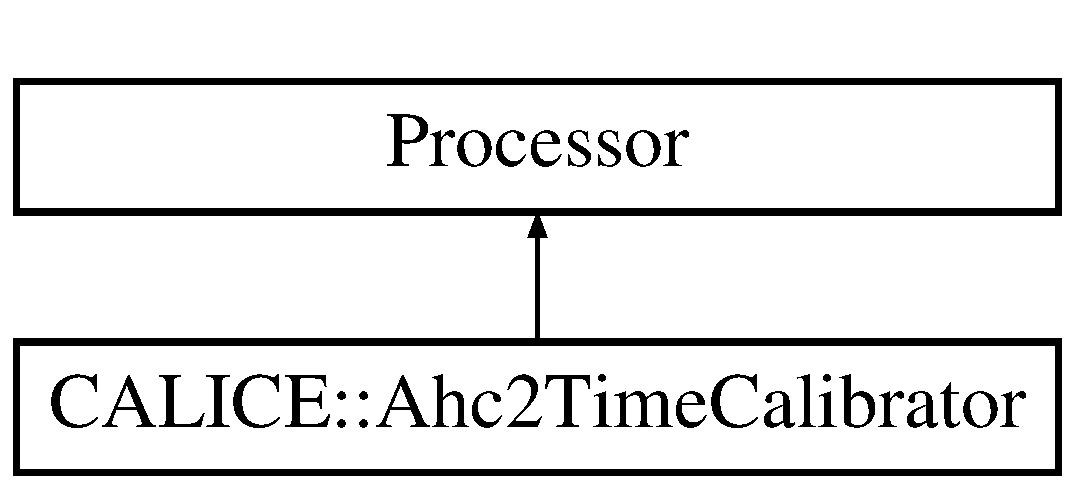
\includegraphics[height=2.000000cm]{classCALICE_1_1Ahc2TimeCalibrator}
\end{center}
\end{figure}
\subsection*{Data Structures}
\begin{DoxyCompactItemize}
\item 
struct {\bf Calib\-Value}
\item 
struct {\bf Hit}
\end{DoxyCompactItemize}
\subsection*{Public Member Functions}
\begin{DoxyCompactItemize}
\item 
{\bf Ahc2\-Time\-Calibrator} $\ast$ {\bfseries new\-Processor} ()\label{classCALICE_1_1Ahc2TimeCalibrator_a62fcfe64c82ded7d6b18a097eac0e227}

\item 
virtual void {\bfseries init} ()\label{classCALICE_1_1Ahc2TimeCalibrator_a1fd9c70b3c5e877cf9453576cdd9fc7f}

\item 
virtual void {\bfseries process\-Event} (L\-C\-Event $\ast$evt)\label{classCALICE_1_1Ahc2TimeCalibrator_a9e46000ab9e97cbf91ed0b5227fecbd1}

\item 
virtual void {\bfseries end} ()\label{classCALICE_1_1Ahc2TimeCalibrator_a2c604dd3e54a64f208d81bfb9fce8677}

\end{DoxyCompactItemize}
\subsection*{Protected Member Functions}
\begin{DoxyCompactItemize}
\item 
void {\bfseries Fill\-Container} (L\-C\-Event $\ast$evt)\label{classCALICE_1_1Ahc2TimeCalibrator_a8f4d7a95735401fbc9f2743fc0c3ac8e}

\item 
{\bf Hit} {\bfseries Read\-Labview\-Block} (const Labview\-Block2 \&block)\label{classCALICE_1_1Ahc2TimeCalibrator_a2039365be1b6ce5fdb18a9daaec4d5f8}

\item 
{\bf Hit} {\bfseries Read\-E\-U\-D\-A\-Q\-Block} (const E\-U\-D\-A\-Q\-Block2016 \&block, int channel)\label{classCALICE_1_1Ahc2TimeCalibrator_a5f2d63f6a2d905854f342adcd97c085d}

\item 
void {\bfseries Process\-Hit} ({\bf Hit} $\ast$hit)\label{classCALICE_1_1Ahc2TimeCalibrator_a9498da3d788f62db60161e3007341163}

\item 
void {\bfseries Fit\-Calibration} ()\label{classCALICE_1_1Ahc2TimeCalibrator_a02b4d7022243d6027d9e39657bdb2935}

\item 
std\-::pair$<$ float, float $>$ {\bfseries calculate\-Slope} (int module\-Nr, int chip\-Nr, int ref\-Mem\-Cell)\label{classCALICE_1_1Ahc2TimeCalibrator_a2a4c34a90bef00000a74b804e82b45ea}

\item 
void {\bfseries Write\-Slopes} (std\-::string fname)\label{classCALICE_1_1Ahc2TimeCalibrator_ab930ac5be7053794d7f2df6bfe680614}

\item 
void {\bfseries Write\-Offsets} (std\-::string fname)\label{classCALICE_1_1Ahc2TimeCalibrator_ac1f9ee17b56d41367cba2a742c6d395e}

\item 
void {\bfseries Write\-Non\-Linearity} (std\-::string fname)\label{classCALICE_1_1Ahc2TimeCalibrator_a744f1b022a5165b0ff981854a15a0fa8}

\item 
void {\bfseries Write\-Time\-Walk} (std\-::string fname)\label{classCALICE_1_1Ahc2TimeCalibrator_a70a98f2549e828f4ef7296d16832312d}

\end{DoxyCompactItemize}
\subsection*{Protected Attributes}
\begin{DoxyCompactItemize}
\item 
std\-::map$<$ int, std\-::map$<$ int, \\*
std\-::map$<$ int, std\-::map$<$ int, \\*
std\-::map$<$ int, std\-::vector\\*
$<$ std\-::pair$<$ float, short $>$ $>$ $>$ $>$ $>$ $>$ $>$ {\bfseries \-\_\-sorted\-Hit\-Container}\label{classCALICE_1_1Ahc2TimeCalibrator_a4ad9a1a2332f58a2c3360f1b445f983b}

\item 
std\-::map$<$ int, std\-::map$<$ int, \\*
std\-::map$<$ int, std\-::map$<$ int, \\*
std\-::map$<$ int, {\bf Calib\-Value} $>$ $>$ $>$ $>$ $>$ {\bfseries \-\_\-m\-\_\-calibration\-\_\-slopes}\label{classCALICE_1_1Ahc2TimeCalibrator_a32d278ad093772556244b07621793fa0}

\item 
std\-::map$<$ int, std\-::map$<$ int, \\*
std\-::map$<$ int, std\-::map$<$ int, \\*
std\-::map$<$ int, {\bf Calib\-Value} $>$ $>$ $>$ $>$ $>$ {\bfseries \-\_\-m\-\_\-calibration\-\_\-offsets}\label{classCALICE_1_1Ahc2TimeCalibrator_a142b706b13a6463b3777ce834866da12}

\item 
std\-::map$<$ int, std\-::map$<$ int, \\*
std\-::map$<$ int, std\-::map$<$ int, \\*
std\-::map$<$ int, {\bf Calib\-Value} $>$ $>$ $>$ $>$ $>$ {\bfseries \-\_\-m\-\_\-calibration\-\_\-non\-Lin\-\_\-\-A}\label{classCALICE_1_1Ahc2TimeCalibrator_a220589cf03693be989b7623ced2c7e9e}

\item 
std\-::map$<$ int, std\-::map$<$ int, \\*
std\-::map$<$ int, std\-::map$<$ int, \\*
std\-::map$<$ int, {\bf Calib\-Value} $>$ $>$ $>$ $>$ $>$ {\bfseries \-\_\-m\-\_\-calibration\-\_\-non\-Lin\-\_\-\-B}\label{classCALICE_1_1Ahc2TimeCalibrator_a9140f56412c2aec3e7124155a051b9a3}

\item 
std\-::map$<$ int, std\-::map$<$ int, \\*
std\-::map$<$ int, std\-::map$<$ int, \\*
std\-::map$<$ int, {\bf Calib\-Value} $>$ $>$ $>$ $>$ $>$ {\bfseries \-\_\-m\-\_\-calibration\-\_\-non\-Lin\-\_\-\-C}\label{classCALICE_1_1Ahc2TimeCalibrator_aa07376af37b1f1a9998c44c530c9be5c}

\item 
std\-::map$<$ int, std\-::map$<$ int, \\*
std\-::map$<$ int, std\-::map$<$ int, \\*
std\-::map$<$ int, {\bf Calib\-Value} $>$ $>$ $>$ $>$ $>$ {\bfseries \-\_\-m\-\_\-calibration\-\_\-time\-Walk\-\_\-\-A}\label{classCALICE_1_1Ahc2TimeCalibrator_ad0a16941e1683907356d77461dd45eba}

\item 
std\-::map$<$ int, std\-::map$<$ int, \\*
std\-::map$<$ int, std\-::map$<$ int, \\*
std\-::map$<$ int, {\bf Calib\-Value} $>$ $>$ $>$ $>$ $>$ {\bfseries \-\_\-m\-\_\-calibration\-\_\-time\-Walk\-\_\-\-B}\label{classCALICE_1_1Ahc2TimeCalibrator_a4db838d0d776f380426f63860bbaa214}

\item 
std\-::map$<$ int, std\-::map$<$ int, \\*
std\-::map$<$ int, std\-::map$<$ int, \\*
std\-::map$<$ int, {\bf Calib\-Value} $>$ $>$ $>$ $>$ $>$ {\bfseries \-\_\-m\-\_\-calibration\-\_\-time\-Walk\-\_\-\-C}\label{classCALICE_1_1Ahc2TimeCalibrator_a17084934e1788a37037f9e130db4bbed}

\item 
int {\bfseries \-\_\-n\-Channels}\label{classCALICE_1_1Ahc2TimeCalibrator_aa5b8cbd07c30249556a8e2a36320d430}

\item 
double {\bfseries \-\_\-tdc\-Error}\label{classCALICE_1_1Ahc2TimeCalibrator_a0f493e5b59d9067a36743f9f680294f0}

\item 
double {\bfseries \-\_\-time\-Reference\-Error}\label{classCALICE_1_1Ahc2TimeCalibrator_aa849707a3a42de7e23c9f4eba28034c5}

\item 
std\-::string {\bf \-\_\-input\-Col\-Name}\label{classCALICE_1_1Ahc2TimeCalibrator_a1f129629f332173ceb51063af096d2c5}

\begin{DoxyCompactList}\small\item\em name of the input collection \end{DoxyCompactList}\item 
std\-::string {\bf \-\_\-ahc\-Hit\-Output\-Col\-Name}\label{classCALICE_1_1Ahc2TimeCalibrator_a7f5d3fd865838898b136b4a67c62947b}

\begin{DoxyCompactList}\small\item\em name of the output A\-H\-C hit collection \end{DoxyCompactList}\item 
std\-::string {\bf \-\_\-mapping\-Processor\-Name}\label{classCALICE_1_1Ahc2TimeCalibrator_a3acabba4b48f6b02b20e620ff5fbfe1e}

\begin{DoxyCompactList}\small\item\em name of the processor which provides the mapping \end{DoxyCompactList}\item 
std\-::string {\bfseries \-\_\-\-Ahc2\-Hardware\-Connection\-Name}\label{classCALICE_1_1Ahc2TimeCalibrator_a1a27e778eeb532c45e45066c8a62e687}

\item 
std\-::string {\bf \-\_\-temperature\-Processor\-Name}\label{classCALICE_1_1Ahc2TimeCalibrator_a4514484c08b455b1aeacdcb9437b5891}

\begin{DoxyCompactList}\small\item\em name of the processor which provides the Si\-P\-M temperature \end{DoxyCompactList}\item 
std\-::string {\bf \-\_\-\-B\-I\-F\-Collection\-Name}\label{classCALICE_1_1Ahc2TimeCalibrator_a6e782c335d79533e8a07de0a4cd9e548}

\begin{DoxyCompactList}\small\item\em name of the processor which provides the Si\-P\-M temperature \end{DoxyCompactList}\item 
int {\bfseries \-\_\-\-B\-I\-F\-Trigger\-Input\-Source}\label{classCALICE_1_1Ahc2TimeCalibrator_a6892b48b05b8004283567cb4b92a4764}

\item 
std\-::string {\bfseries \-\_\-reference\-Time\-Type}\label{classCALICE_1_1Ahc2TimeCalibrator_ab5b5c93d447b33cac8235999fd187653}

\item 
std\-::string {\bfseries \-\_\-output\-File\-Name\-\_\-time\-Slopes}\label{classCALICE_1_1Ahc2TimeCalibrator_a56cdc5e9bc932c58edbd46c3bbca5230}

\item 
std\-::string {\bfseries \-\_\-output\-File\-Name\-\_\-time\-Offsets}\label{classCALICE_1_1Ahc2TimeCalibrator_a408ffd6f123e860d267744f7fa894783}

\item 
std\-::string {\bfseries \-\_\-output\-File\-Name\-\_\-time\-Non\-Linearity}\label{classCALICE_1_1Ahc2TimeCalibrator_a4ebb2345b37be10960e788ff9fb1160e}

\item 
std\-::string {\bfseries \-\_\-output\-File\-Name\-\_\-time\-Walk}\label{classCALICE_1_1Ahc2TimeCalibrator_a7366ba658069d92b966e321aa340fb31}

\item 
bool {\bfseries \-\_\-skip\-First\-Memory\-Cell}\label{classCALICE_1_1Ahc2TimeCalibrator_aa4d1078711558d163eeb66822d8dd94a}

\item 
int {\bfseries \-\_\-min\-Hits\-Fit}\label{classCALICE_1_1Ahc2TimeCalibrator_a79c2ba9abf8dea2d2a8c7d197dde52c2}

\item 
int {\bfseries \-\_\-max\-Hits\-Fit}\label{classCALICE_1_1Ahc2TimeCalibrator_a866c3efc071b29bcdf8a3d4e12539cc9}

\item 
std\-::string {\bf \-\_\-cell\-Description\-Processor\-Name}\label{classCALICE_1_1Ahc2TimeCalibrator_a36014aff492d28ca737829e1158c9a4b}

\begin{DoxyCompactList}\small\item\em name of the processor which provides the cells description \end{DoxyCompactList}\item 
Mapped\-Container\\*
$<$ Cell\-Description $>$ $\ast$ {\bf \-\_\-cell\-Descriptions}\label{classCALICE_1_1Ahc2TimeCalibrator_abe7c15147b77f585c769a7e1dc017af2}

\begin{DoxyCompactList}\small\item\em mapped container of cells description \end{DoxyCompactList}\item 
const Mapper $\ast$ {\bf \-\_\-mapper}\label{classCALICE_1_1Ahc2TimeCalibrator_a64c2d4119029e9ce8a77047b7b545c6c}

\begin{DoxyCompactList}\small\item\em the mapper \end{DoxyCompactList}\item 
Mapped\-Container$<$ Simple\-Value $>$ $\ast$ {\bf \-\_\-temperature\-Container}\label{classCALICE_1_1Ahc2TimeCalibrator_ade953481012d4286540e924df6e50165}

\begin{DoxyCompactList}\small\item\em mapped container of cells temperature \end{DoxyCompactList}\item 
bool {\bf \-\_\-newdataformat}\label{classCALICE_1_1Ahc2TimeCalibrator_ade5aaf5f3727eb0ee1e1d9dd1c4d484d}

\begin{DoxyCompactList}\small\item\em flag for the new data format in E\-U\-D\-A\-Q \end{DoxyCompactList}\item 
bool {\bf \-\_\-is\-First\-Event}
\begin{DoxyCompactList}\small\item\em flag to switch to D\-A\-T\-A/\-M\-C at the first event, the following events should be the same. \end{DoxyCompactList}\item 
Mapped\-Container\\*
$<$ Calorimeter\-Hit\-Impl $>$ $\ast$ {\bf \-\_\-\-Hit\-Container}\label{classCALICE_1_1Ahc2TimeCalibrator_a7627ab3a3eb5245b1500a5a228bd3ccb}

\begin{DoxyCompactList}\small\item\em mapped container of A\-H\-C\-A\-L cells \end{DoxyCompactList}\item 
std\-::map$<$ int, std\-::pair$<$ int, \\*
int $>$ $>$ {\bf \-\_\-\-Hardware\-Connnection\-Container}\label{classCALICE_1_1Ahc2TimeCalibrator_aa91b9bbcb6a6a3be99515647e895e611}

\begin{DoxyCompactList}\small\item\em map containing relationship between Chip\-I\-D and Module/\-Chip\-Nb \end{DoxyCompactList}\item 
int {\bfseries \-\_\-i\-Evt} = 0\label{classCALICE_1_1Ahc2TimeCalibrator_a2441a8d16fa6b8f36d6ffbbe2bccfe85}

\end{DoxyCompactItemize}


\subsection{Detailed Description}
Processor that does the Si\-P\-M calibration. 

The calibration is done according to the formula\-: $E_{calibrated}=f_{saturation}((E_{raw}-pedestal) \cdot IC/gain) \cdot gain/IC/MIP$

Please note\-:
\begin{DoxyItemize}
\item this processor does the calibration for both data and Monte Carlo, based on the type of the input collection (\char`\"{}\-L\-C\-Generic\-Object\char`\"{} for data, and \char`\"{}\-Calorimeter\-Hit\char`\"{} for Monte Carlo);
\item for noise creation, the saturation correction is disabled (do\-Saturation\-Correction=false), as well as the Zero\-Suppression (Zero\-Suppression = false)
\item for Monte Carlo, the pedestal subtraction is disabled (Pedestal\-Subtraction=false)
\end{DoxyItemize}

\begin{DoxyParagraph}{processor parameters}
\begin{TabularC}{2}
\hline
steering file parameter name &description  \\\cline{1-2}
{\bfseries {\itshape  Input\-Collection\-Name }}&name of the input collection, with energy in A\-D\-C counts \\\cline{1-2}
{\bfseries {\itshape  Output\-Collection\-Name }}&name of the output collection, with energy in M\-I\-Ps \\\cline{1-2}
{\bfseries {\itshape  Mapping\-Processor\-Name }}&name of the mapping processor that provides the necessary Mapper class \\\cline{1-2}
{\bfseries {\itshape  Ahc2\-Calibrations\-Processor\-Name }}&name of the processor which provides the Si\-P\-M calibrations \\\cline{1-2}
{\bfseries {\itshape  Si\-P\-M\-Temperature\-Processor\-Name }}&name of the processor which provides the Si\-P\-M temperature \\\cline{1-2}
{\bfseries {\itshape  Pedestal\-Subtraction }}&Flag to enable/disable pedestal subtraction \\\cline{1-2}
{\bfseries {\itshape  Zero\-Suppression }}&Flag to enable/disable zero suppression (intention to apply the M\-I\-P cut) \\\cline{1-2}
{\bfseries {\itshape  Mip\-Cut }}&Value of the M\-I\-P cut (default\-: 0.\-4 M\-I\-Ps) \\\cline{1-2}
{\bfseries {\itshape  do\-Mip\-Conversion }}&Flag to enable/disable M\-I\-P Calibration \\\cline{1-2}
{\bfseries {\itshape  do\-Mip\-Temperature\-Correction }}&Flag to enable/disable temperature correction of the M\-I\-P \\\cline{1-2}
{\bfseries {\itshape  do\-Gain\-Temperature\-Correction }}&Flag to enable/disable temperature correction of the gain \\\cline{1-2}
{\bfseries {\itshape  do\-Saturation\-Correction }}&Flag to enable/disable the saturation correction \\\cline{1-2}
{\bfseries {\itshape  do\-Time\-Conversion }}&Flag to enable/disable the T\-D\-C Calibration \\\cline{1-2}
{\bfseries {\itshape  do\-Error\-Calculation }}&Flag to enable/disable error calculation \\\cline{1-2}
{\bfseries {\itshape  filter\-Dead\-Cells }}&Flag to enable/disable the filtering of dead cells \\\cline{1-2}
{\bfseries {\itshape  filter\-Default\-Cells }}&Flag to enable/disable the filtering of default dead cells \\\cline{1-2}
\end{TabularC}

\end{DoxyParagraph}
\begin{DoxyAuthor}{Author}
{\tt cgraf@mpp.\-mpg.\-de} 
\end{DoxyAuthor}
\begin{DoxyVersion}{Version}
0.\-1 
\end{DoxyVersion}
\begin{DoxyDate}{Date}
January 2018 
\end{DoxyDate}


Definition at line 63 of file Ahc2\-Time\-Calibrator.\-hh.



\subsection{Field Documentation}
\index{C\-A\-L\-I\-C\-E\-::\-Ahc2\-Time\-Calibrator@{C\-A\-L\-I\-C\-E\-::\-Ahc2\-Time\-Calibrator}!\-\_\-is\-First\-Event@{\-\_\-is\-First\-Event}}
\index{\-\_\-is\-First\-Event@{\-\_\-is\-First\-Event}!CALICE::Ahc2TimeCalibrator@{C\-A\-L\-I\-C\-E\-::\-Ahc2\-Time\-Calibrator}}
\subsubsection[{\-\_\-is\-First\-Event}]{\setlength{\rightskip}{0pt plus 5cm}bool C\-A\-L\-I\-C\-E\-::\-Ahc2\-Time\-Calibrator\-::\-\_\-is\-First\-Event\hspace{0.3cm}{\ttfamily [protected]}}\label{classCALICE_1_1Ahc2TimeCalibrator_a5f7e021c927d01063e9ec177deec463c}


flag to switch to D\-A\-T\-A/\-M\-C at the first event, the following events should be the same. 



Definition at line 182 of file Ahc2\-Time\-Calibrator.\-hh.



The documentation for this class was generated from the following files\-:\begin{DoxyCompactItemize}
\item 
Ahc2\-Time\-Calibrator.\-hh\item 
Ahc2\-Time\-Calibrator.\-cc\end{DoxyCompactItemize}

\section{C\-A\-L\-I\-C\-E\-:\-:Angle\-Track\-Finder Class Reference}
\label{classCALICE_1_1AngleTrackFinder}\index{C\-A\-L\-I\-C\-E\-::\-Angle\-Track\-Finder@{C\-A\-L\-I\-C\-E\-::\-Angle\-Track\-Finder}}


Processor to extract M\-I\-P calibrations from muon beam runs.  




{\ttfamily \#include $<$Angle\-Track\-Finder.\-hh$>$}

Inheritance diagram for C\-A\-L\-I\-C\-E\-:\-:Angle\-Track\-Finder\-:\begin{figure}[H]
\begin{center}
\leavevmode
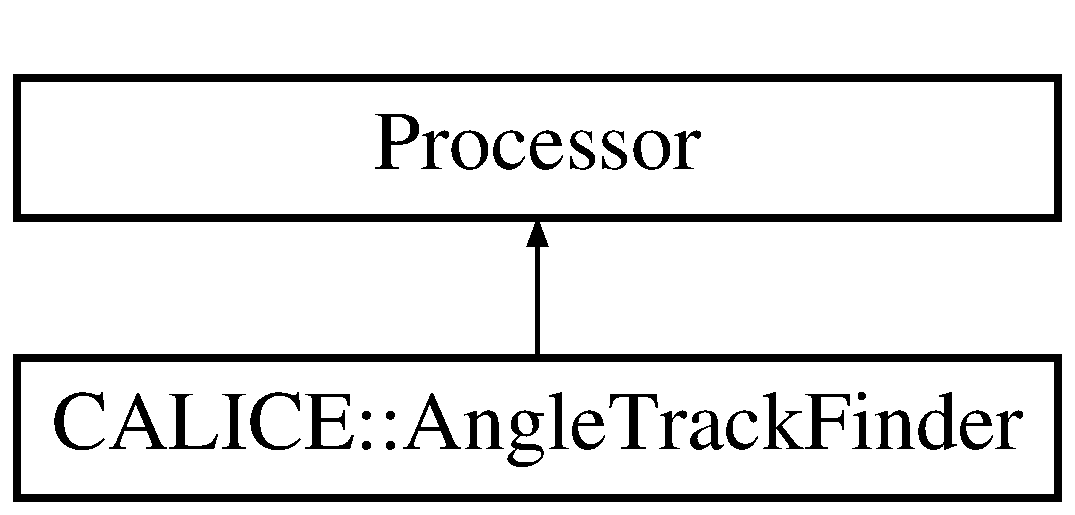
\includegraphics[height=2.000000cm]{classCALICE_1_1AngleTrackFinder}
\end{center}
\end{figure}
\subsection*{Public Member Functions}
\begin{DoxyCompactItemize}
\item 
virtual Processor $\ast$ {\bf new\-Processor} ()\label{classCALICE_1_1AngleTrackFinder_af929a19d0689fbf8f946988797daff4a}

\begin{DoxyCompactList}\small\item\em Return new instance of this processor. \end{DoxyCompactList}\item 
{\bf Angle\-Track\-Finder} ()\label{classCALICE_1_1AngleTrackFinder_a74cdcf69ca7ef1072ccdd5ea7d9ae551}

\begin{DoxyCompactList}\small\item\em Default constructor. \end{DoxyCompactList}\item 
{\bf $\sim$\-Angle\-Track\-Finder} ()\label{classCALICE_1_1AngleTrackFinder_acf657623bf1eff4c45b4af704f519ca3}

\begin{DoxyCompactList}\small\item\em Destructor. \end{DoxyCompactList}\item 
virtual void {\bf init} ()\label{classCALICE_1_1AngleTrackFinder_a994a129403fc067c93e4a37545c79499}

\begin{DoxyCompactList}\small\item\em Initialise useful variables. \end{DoxyCompactList}\item 
virtual void {\bf process\-Event} (L\-C\-Event $\ast$evt)
\begin{DoxyCompactList}\small\item\em Process event (the working horse) \end{DoxyCompactList}\item 
virtual void {\bf end} ()\label{classCALICE_1_1AngleTrackFinder_a4e7d844d0f42764d16f9f66a3f887f4c}

\begin{DoxyCompactList}\small\item\em Function to be called at the end of the job, after all events have been processed, for clean up. \end{DoxyCompactList}\end{DoxyCompactItemize}
\subsection*{Private Member Functions}
\begin{DoxyCompactItemize}
\item 
void {\bf open\-Input\-Collections} (L\-C\-Event $\ast$evt)
\begin{DoxyCompactList}\small\item\em Open the input collections. \end{DoxyCompactList}\item 
void {\bf find\-Track} (L\-C\-Event $\ast$evt)
\begin{DoxyCompactList}\small\item\em Find the track. \end{DoxyCompactList}\item 
bool {\bf do\-Further\-Analysis} ()
\begin{DoxyCompactList}\small\item\em Check if cuts are fullfilled, and if analysis is to be continued. \end{DoxyCompactList}\item 
std\-::vector$<$ Calorimeter\-Hit $\ast$ $>$ {\bf extract\-A\-H\-C\-A\-L\-Information} ()\label{classCALICE_1_1AngleTrackFinder_a86fc7e637d10c7ee1ab9851b1fc54e1b}

\begin{DoxyCompactList}\small\item\em Extract A\-H\-C\-A\-L information. \end{DoxyCompactList}\item 
std\-::pair$<$ int, float $>$ {\bf extract\-Number\-Of\-Hits\-And\-Energy\-Sum} (L\-C\-Collection $\ast$input\-Col)
\begin{DoxyCompactList}\small\item\em Extract number of hits and the energy sum from the input collection. \end{DoxyCompactList}\item 
void {\bf find\-Track\-Clusters} (std\-::vector$<$ Calorimeter\-Hit $\ast$ $>$ \&hcal\-Vec, E\-V\-E\-N\-T\-::\-Cluster\-Vec \&output\-Vec)
\begin{DoxyCompactList}\small\item\em Find clusters of M\-I\-P tracks. \end{DoxyCompactList}\item 
void {\bfseries find\-Track\-Clusters\-Coarse} (std\-::vector$<$ Calorimeter\-Hit $\ast$ $>$ \&hcal\-Vec, E\-V\-E\-N\-T\-::\-Cluster\-Vec \&output\-Vec)\label{classCALICE_1_1AngleTrackFinder_a2a052d786ad1c5defe012d580f9da5d1}

\item 
E\-V\-E\-N\-T\-::\-Cluster\-Vec {\bfseries extend\-Tracks\-To\-Tcmt} (L\-C\-Typed\-Vector$<$ Calorimeter\-Hit $>$ $\ast$tcmt\-Vec, E\-V\-E\-N\-T\-::\-Cluster\-Vec track\-Clusters)\label{classCALICE_1_1AngleTrackFinder_a184c520d08cc8dde4c813bc44784ca52}

\item 
void {\bf select\-Track\-Clusters} (E\-V\-E\-N\-T\-::\-Cluster\-Vec cluster\-Vec, const std\-::string track\-Selection\-Mode, E\-V\-E\-N\-T\-::\-Cluster\-Vec \&good\-Track\-Clusters)
\begin{DoxyCompactList}\small\item\em Select good tracks. \end{DoxyCompactList}\item 
void {\bfseries merge\-Coarse\-Clusters} (E\-V\-E\-N\-T\-::\-Cluster\-Vec goodcluster\-Vec, E\-V\-E\-N\-T\-::\-Cluster\-Vec cluster\-Coarse\-Vec, E\-V\-E\-N\-T\-::\-Cluster\-Vec \&output\-Vec, const std\-::string track\-Selection\-Mode)\label{classCALICE_1_1AngleTrackFinder_ad57cb7c54e211b1f6c79904a45611903}

\item 
Cluster\-Impl $\ast$ {\bf get\-Whole\-Track} (Cluster $\ast$track\-Cluster)
\begin{DoxyCompactList}\small\item\em Get the whole track (i.\-e. \end{DoxyCompactList}\item 
Cluster\-Impl $\ast$ {\bfseries get\-Whole\-Track\-Segment} (Cluster $\ast$track\-Cluster)\label{classCALICE_1_1AngleTrackFinder_a30c444b8e888a60ca81305ddadda9c83}

\item 
Cluster\-Impl $\ast$ {\bfseries copy\-A\-Cluster} (Cluster $\ast$track\-Cluster)\label{classCALICE_1_1AngleTrackFinder_a0769f3c37445bf0e8efce89f90049814}

\item 
E\-V\-E\-N\-T\-::\-Cluster\-Vec {\bf get\-Remaining\-Hits} (E\-V\-E\-N\-T\-::\-Cluster\-Vec selected\-Track\-Clusters)
\begin{DoxyCompactList}\small\item\em Get the vector of track clusters containing all the remaining hits. \end{DoxyCompactList}\item 
E\-V\-E\-N\-T\-::\-Cluster\-Vec {\bfseries get\-Remaining\-Hits\-Of\-Track\-Segment} (E\-V\-E\-N\-T\-::\-Cluster\-Vec selected\-Track\-Clusters)\label{classCALICE_1_1AngleTrackFinder_a13fdc56df9fcf40ed6bd8dad70ee200e}

\item 
E\-V\-E\-N\-T\-::\-Cluster\-Vec {\bfseries get\-Final\-Cluster} (E\-V\-E\-N\-T\-::\-Cluster\-Vec selected\-Track\-Clusters)\label{classCALICE_1_1AngleTrackFinder_af37cc1b4e139645ca4578d224f019fd3}

\item 
void {\bf create\-Output\-Collection} (L\-C\-Event $\ast$evt, E\-V\-E\-N\-T\-::\-Cluster\-Vec final\-Vec)
\begin{DoxyCompactList}\small\item\em Create output collection of track clusters. \end{DoxyCompactList}\item 
E\-V\-E\-N\-T\-::\-Cluster\-Vec {\bfseries obtain\-Sub\-Clusters} (E\-V\-E\-N\-T\-::\-Cluster $\ast$cluster\-A)\label{classCALICE_1_1AngleTrackFinder_add0057082ccc0bcea73c30d9926fe317}

\item 
E\-V\-E\-N\-T\-::\-Cluster\-Vec {\bfseries remove\-Isolated\-Hits} (E\-V\-E\-N\-T\-::\-Cluster\-Vec sub\-Cluster)\label{classCALICE_1_1AngleTrackFinder_a1af99dd0d0e7dc58b6a1348a5d3729fd}

\item 
bool {\bfseries check\-X\-Y\-Adjacent\-Clusters} (Cluster $\ast$cluster\-A, Cluster $\ast$cluster\-B, int num\-Of\-Adjacent\-Cells)\label{classCALICE_1_1AngleTrackFinder_a1786792116034051608781193e344134}

\end{DoxyCompactItemize}
\subsection*{Private Attributes}
\begin{DoxyCompactItemize}
\item 
const Mapper $\ast$ {\bf \-\_\-mapper}\label{classCALICE_1_1AngleTrackFinder_a1e8ade0f953c3f0e73665cf8bb6fc58f}

\begin{DoxyCompactList}\small\item\em the mapper \end{DoxyCompactList}\item 
std\-::string {\bf \-\_\-mapping\-Processor\-Name}\label{classCALICE_1_1AngleTrackFinder_a8ed332f4a4fac3a16df92f32cec1ca23}

\begin{DoxyCompactList}\small\item\em name of the processor which provides the mapping \end{DoxyCompactList}\item 
std\-::string {\bf \-\_\-cell\-Description\-Processor\-Name}\label{classCALICE_1_1AngleTrackFinder_a9094f5b2aa449c3bd3180fe4fc7094d2}

\begin{DoxyCompactList}\small\item\em name of the processor which provides the cells description \end{DoxyCompactList}\item 
Mapped\-Container\\*
$<$ C\-A\-L\-I\-C\-E\-::\-Cell\-Description $>$ $\ast$ {\bfseries \-\_\-cell\-Descriptions}\label{classCALICE_1_1AngleTrackFinder_a570dfea9f64f3eaf487ea8db682d03ec}

\item 
L\-C\-Collection $\ast$ {\bf \-\_\-ecal\-Input\-Col}\label{classCALICE_1_1AngleTrackFinder_a6c55f00b24dedf933046c374d57567a2}

\begin{DoxyCompactList}\small\item\em E\-C\-A\-L input collection. \end{DoxyCompactList}\item 
L\-C\-Collection $\ast$ {\bf \-\_\-ahcal\-Input\-Col}\label{classCALICE_1_1AngleTrackFinder_a6294fed90962d5ecaf2d63f4f119c808}

\begin{DoxyCompactList}\small\item\em A\-H\-C\-A\-L input collection. \end{DoxyCompactList}\item 
L\-C\-Collection $\ast$ {\bf \-\_\-ahcal\-Amp\-Input\-Col}\label{classCALICE_1_1AngleTrackFinder_a63d915b7e5159274be1cec89db2c0390}

\begin{DoxyCompactList}\small\item\em A\-H\-C\-A\-L Amplitude input collection. \end{DoxyCompactList}\item 
L\-C\-Collection $\ast$ {\bf \-\_\-tcmt\-Input\-Col}\label{classCALICE_1_1AngleTrackFinder_a961a3ce5cad59157ae7cc350da27017b}

\begin{DoxyCompactList}\small\item\em T\-C\-M\-T input collection. \end{DoxyCompactList}\item 
std\-::string {\bfseries \-\_\-ecal\-Input\-Col\-Name}\label{classCALICE_1_1AngleTrackFinder_aa226f88b009a6d2f77c4b8c863579ac1}

\item 
std\-::string {\bfseries \-\_\-ahcal\-Input\-Col\-Name}\label{classCALICE_1_1AngleTrackFinder_af139ab1be231e5e7daa0d72c3b05ce27}

\item 
std\-::string {\bfseries \-\_\-ahcal\-Amp\-Input\-Col\-Name}\label{classCALICE_1_1AngleTrackFinder_a00c257e37403fb1209fcded626033de5}

\item 
std\-::string {\bfseries \-\_\-ahcal\-Output\-Track\-Col\-Name}\label{classCALICE_1_1AngleTrackFinder_afcc15eae818bff82cb07f8a206b4eb6b}

\item 
std\-::string {\bfseries \-\_\-tcmt\-Output\-Track\-Col\-Name}\label{classCALICE_1_1AngleTrackFinder_afc39c68fdbd2e58a0ae729952f6c307e}

\item 
std\-::string {\bfseries \-\_\-tcmt\-Input\-Col\-Name}\label{classCALICE_1_1AngleTrackFinder_af55dd53460826abc6abe7eb4917f201b}

\item 
std\-::string {\bfseries \-\_\-encoding\-String}\label{classCALICE_1_1AngleTrackFinder_aec98c28c81cf10cb1fd7d83bbe560120}

\item 
std\-::string {\bf \-\_\-track\-Selection\-Mode}\label{classCALICE_1_1AngleTrackFinder_a9e65faf8074db90de8771bc2dccf072c}

\begin{DoxyCompactList}\small\item\em track selection mode\-: N\-H\-I\-Ts = based on the number of hits; P\-E\-R\-P\-E\-N\-D\-I\-C\-U\-L\-A\-R = select only perpendicular tracks \end{DoxyCompactList}\item 
L\-C\-Relation\-Navigator $\ast$ {\bfseries \-\_\-navigator}\label{classCALICE_1_1AngleTrackFinder_adb33fe8149d97611b8eb62037138f972}

\item 
E\-V\-E\-N\-T\-::\-Cluster\-Vec {\bfseries \-\_\-good\-Track\-Clusters}\label{classCALICE_1_1AngleTrackFinder_a7218355d693e3d50095b7a5370bec077}

\item 
bool {\bfseries \-\_\-use\-E\-C\-A\-L}\label{classCALICE_1_1AngleTrackFinder_a1590732ddda798d70bb97bd886a0bc22}

\item 
bool {\bfseries \-\_\-use\-T\-C\-M\-T}\label{classCALICE_1_1AngleTrackFinder_aad59f9038d2f9935f0dd0bd5b9700ed3}

\item 
bool {\bfseries \-\_\-tcmt\-Start\-Vertical}\label{classCALICE_1_1AngleTrackFinder_a7f12d1a7817b3ee3686eefcf70fa0049}

\item 
float {\bfseries \-\_\-tcmt\-Strip\-Width}\label{classCALICE_1_1AngleTrackFinder_a1f5753f67ba97ef9aeb4cb57f75ff309}

\item 
bool {\bf \-\_\-is\-Non\-Muon\-Run}\label{classCALICE_1_1AngleTrackFinder_a599998d50ef67e2bc2e9a07b0864dd3d}

\begin{DoxyCompactList}\small\item\em flag for non-\/muon run \end{DoxyCompactList}\item 
int {\bf \-\_\-ahcal\-Max\-No\-Hits}\label{classCALICE_1_1AngleTrackFinder_a94a071cd5fbe48451c8aace1168f9697}

\begin{DoxyCompactList}\small\item\em maximum number of hits in the A\-H\-C\-A\-L \end{DoxyCompactList}\item 
int {\bf \-\_\-ecal\-Min\-No\-Hits}\label{classCALICE_1_1AngleTrackFinder_a5db8580f90e8193fad643ca4415260ab}

\begin{DoxyCompactList}\small\item\em minimum number of hits in the E\-C\-A\-L \end{DoxyCompactList}\item 
int {\bf \-\_\-ecal\-Max\-No\-Hits}\label{classCALICE_1_1AngleTrackFinder_a305795d0103cb33c9cf579d83d050968}

\begin{DoxyCompactList}\small\item\em maximum number of hits in the E\-C\-A\-L \end{DoxyCompactList}\item 
float {\bf \-\_\-tcmt\-Min\-Energy\-Sum}\label{classCALICE_1_1AngleTrackFinder_ab5ac7f274d7c9936f4d19ed1ac463715}

\begin{DoxyCompactList}\small\item\em minimum energy sum in the T\-C\-M\-T \end{DoxyCompactList}\item 
float {\bf \-\_\-mip\-Cut\-Value}\label{classCALICE_1_1AngleTrackFinder_a09632c19bf97a231d9ab2c1e6e32cc78}

\begin{DoxyCompactList}\small\item\em M\-I\-P cut value (0.\-5 M\-I\-Ps) \end{DoxyCompactList}\item 
int {\bfseries \-\_\-mip\-Cut\-Variable}\label{classCALICE_1_1AngleTrackFinder_afeb7153710a99c4b36d0842d2df63335}

\item 
int {\bf \-\_\-track\-No\-Hits\-Threshold}
\begin{DoxyCompactList}\small\item\em choose amplitude to be used to perform the mip cut \end{DoxyCompactList}\item 
int {\bfseries \-\_\-use\-Coarse\-Section}\label{classCALICE_1_1AngleTrackFinder_acbeb9d16089487bbc26fa28c1a83ca78}

\item 
int {\bfseries \-\_\-min\-Active\-T\-C\-M\-T\-Parallel\-Strips}\label{classCALICE_1_1AngleTrackFinder_ac050b4b2a689ca4d482a6ad75a53991c}

\item 
Int\-Vec {\bf \-\_\-bad\-Ahcal\-Modules\-Vec}\label{classCALICE_1_1AngleTrackFinder_a6d4442136ce5b168d27f32f3f753164c}

\begin{DoxyCompactList}\small\item\em vector of bad A\-H\-C\-A\-L modules numbers \end{DoxyCompactList}\item 
Int\-Vec {\bf \-\_\-first\-Ahcal\-Modules\-Vec}\label{classCALICE_1_1AngleTrackFinder_a53176eb4d890fcf6f41291a7aa7f7ecd}

\begin{DoxyCompactList}\small\item\em vector of numbers of the beginning A\-H\-C\-A\-L modules which are used for perpendicular track finding \end{DoxyCompactList}\item 
Int\-Vec {\bf \-\_\-last\-Ahcal\-Modules\-Vec}\label{classCALICE_1_1AngleTrackFinder_afe5e51f2a91a84dabaed6f6ad9cd60e9}

\begin{DoxyCompactList}\small\item\em vector of numbers of the ending A\-H\-C\-A\-L modules which are used for perpendicular track finding \end{DoxyCompactList}\item 
E\-V\-E\-N\-T\-::\-Calorimeter\-Hit\-Vec {\bf \-\_\-all\-Ahcal\-Hits\-In\-Event\-Vec}\label{classCALICE_1_1AngleTrackFinder_aef20f858c612a3181537606fdc4be0f1}

\begin{DoxyCompactList}\small\item\em vector containing all A\-H\-C\-A\-L hits from the event \end{DoxyCompactList}\end{DoxyCompactItemize}
\subsection*{Static Private Attributes}
\begin{DoxyCompactItemize}
\item 
static const unsigned int {\bfseries M\-A\-X\-T\-C\-M\-T\-L\-A\-Y\-E\-R\-S} = 16\label{classCALICE_1_1AngleTrackFinder_a42ed04f962d4a3564dbcb4811cd4f21b}

\item 
static const unsigned int {\bfseries M\-A\-X\-T\-C\-M\-T\-S\-T\-R\-I\-P\-S} = 20\label{classCALICE_1_1AngleTrackFinder_ad99874d9a4bd40c23336a9740c34bb23}

\end{DoxyCompactItemize}


\subsection{Detailed Description}
Processor to extract M\-I\-P calibrations from muon beam runs. 

\begin{DoxyAuthor}{Author}
A.\-Vargas D\-E\-S\-Y 
\end{DoxyAuthor}
\begin{DoxyDate}{Date}
November 2010 
\end{DoxyDate}


Definition at line 35 of file Angle\-Track\-Finder.\-hh.



\subsection{Member Function Documentation}
\index{C\-A\-L\-I\-C\-E\-::\-Angle\-Track\-Finder@{C\-A\-L\-I\-C\-E\-::\-Angle\-Track\-Finder}!create\-Output\-Collection@{create\-Output\-Collection}}
\index{create\-Output\-Collection@{create\-Output\-Collection}!CALICE::AngleTrackFinder@{C\-A\-L\-I\-C\-E\-::\-Angle\-Track\-Finder}}
\subsubsection[{create\-Output\-Collection}]{\setlength{\rightskip}{0pt plus 5cm}void C\-A\-L\-I\-C\-E\-::\-Angle\-Track\-Finder\-::create\-Output\-Collection (
\begin{DoxyParamCaption}
\item[{L\-C\-Event $\ast$}]{evt, }
\item[{E\-V\-E\-N\-T\-::\-Cluster\-Vec}]{final\-Vec}
\end{DoxyParamCaption}
)\hspace{0.3cm}{\ttfamily [private]}}\label{classCALICE_1_1AngleTrackFinder_ae2aa960da701d5e62b15e21c1df40691}


Create output collection of track clusters. 


\begin{DoxyParams}{Parameters}
{\em evt} & the processed event \\
\hline
{\em final\-Vec} & final vector of track clusters, after all selections \\
\hline
\end{DoxyParams}


Definition at line 1204 of file Angle\-Track\-Finder.\-cc.



References \-\_\-tcmt\-Input\-Col.



Referenced by find\-Track().

\index{C\-A\-L\-I\-C\-E\-::\-Angle\-Track\-Finder@{C\-A\-L\-I\-C\-E\-::\-Angle\-Track\-Finder}!do\-Further\-Analysis@{do\-Further\-Analysis}}
\index{do\-Further\-Analysis@{do\-Further\-Analysis}!CALICE::AngleTrackFinder@{C\-A\-L\-I\-C\-E\-::\-Angle\-Track\-Finder}}
\subsubsection[{do\-Further\-Analysis}]{\setlength{\rightskip}{0pt plus 5cm}bool C\-A\-L\-I\-C\-E\-::\-Angle\-Track\-Finder\-::do\-Further\-Analysis (
\begin{DoxyParamCaption}
{}
\end{DoxyParamCaption}
)\hspace{0.3cm}{\ttfamily [private]}}\label{classCALICE_1_1AngleTrackFinder_a118f2d1e9c47337831da14c8c356e555}


Check if cuts are fullfilled, and if analysis is to be continued. 

\begin{DoxyReturn}{Returns}
analyse flag to show if the cuts are fullfilled or not 
\end{DoxyReturn}


Definition at line 377 of file Angle\-Track\-Finder.\-cc.



References \-\_\-ahcal\-Input\-Col, \-\_\-ahcal\-Max\-No\-Hits, \-\_\-ecal\-Input\-Col, \-\_\-ecal\-Max\-No\-Hits, \-\_\-ecal\-Min\-No\-Hits, \-\_\-is\-Non\-Muon\-Run, \-\_\-tcmt\-Input\-Col, \-\_\-tcmt\-Min\-Energy\-Sum, and extract\-Number\-Of\-Hits\-And\-Energy\-Sum().



Referenced by find\-Track().

\index{C\-A\-L\-I\-C\-E\-::\-Angle\-Track\-Finder@{C\-A\-L\-I\-C\-E\-::\-Angle\-Track\-Finder}!extract\-Number\-Of\-Hits\-And\-Energy\-Sum@{extract\-Number\-Of\-Hits\-And\-Energy\-Sum}}
\index{extract\-Number\-Of\-Hits\-And\-Energy\-Sum@{extract\-Number\-Of\-Hits\-And\-Energy\-Sum}!CALICE::AngleTrackFinder@{C\-A\-L\-I\-C\-E\-::\-Angle\-Track\-Finder}}
\subsubsection[{extract\-Number\-Of\-Hits\-And\-Energy\-Sum}]{\setlength{\rightskip}{0pt plus 5cm}std\-::pair$<$ int, float $>$ C\-A\-L\-I\-C\-E\-::\-Angle\-Track\-Finder\-::extract\-Number\-Of\-Hits\-And\-Energy\-Sum (
\begin{DoxyParamCaption}
\item[{L\-C\-Collection $\ast$}]{input\-Col}
\end{DoxyParamCaption}
)\hspace{0.3cm}{\ttfamily [private]}}\label{classCALICE_1_1AngleTrackFinder_a1799da6da5db2cbf5de0e458ccbe3566}


Extract number of hits and the energy sum from the input collection. 


\begin{DoxyParams}{Parameters}
{\em input\-Col} & the input collection \\
\hline
\end{DoxyParams}


Definition at line 457 of file Angle\-Track\-Finder.\-cc.



Referenced by do\-Further\-Analysis().

\index{C\-A\-L\-I\-C\-E\-::\-Angle\-Track\-Finder@{C\-A\-L\-I\-C\-E\-::\-Angle\-Track\-Finder}!find\-Track@{find\-Track}}
\index{find\-Track@{find\-Track}!CALICE::AngleTrackFinder@{C\-A\-L\-I\-C\-E\-::\-Angle\-Track\-Finder}}
\subsubsection[{find\-Track}]{\setlength{\rightskip}{0pt plus 5cm}void C\-A\-L\-I\-C\-E\-::\-Angle\-Track\-Finder\-::find\-Track (
\begin{DoxyParamCaption}
\item[{L\-C\-Event $\ast$}]{evt}
\end{DoxyParamCaption}
)\hspace{0.3cm}{\ttfamily [private]}}\label{classCALICE_1_1AngleTrackFinder_aac50b453e10cdfbb6612eeefcb5ca25c}


Find the track. 


\begin{DoxyParams}{Parameters}
{\em evt} & event to be processed \\
\hline
\end{DoxyParams}


Definition at line 271 of file Angle\-Track\-Finder.\-cc.



References \-\_\-ahcal\-Max\-No\-Hits, \-\_\-tcmt\-Input\-Col, \-\_\-track\-Selection\-Mode, create\-Output\-Collection(), do\-Further\-Analysis(), extract\-A\-H\-C\-A\-L\-Information(), find\-Track\-Clusters(), and select\-Track\-Clusters().



Referenced by process\-Event().

\index{C\-A\-L\-I\-C\-E\-::\-Angle\-Track\-Finder@{C\-A\-L\-I\-C\-E\-::\-Angle\-Track\-Finder}!find\-Track\-Clusters@{find\-Track\-Clusters}}
\index{find\-Track\-Clusters@{find\-Track\-Clusters}!CALICE::AngleTrackFinder@{C\-A\-L\-I\-C\-E\-::\-Angle\-Track\-Finder}}
\subsubsection[{find\-Track\-Clusters}]{\setlength{\rightskip}{0pt plus 5cm}void C\-A\-L\-I\-C\-E\-::\-Angle\-Track\-Finder\-::find\-Track\-Clusters (
\begin{DoxyParamCaption}
\item[{std\-::vector$<$ Calorimeter\-Hit $\ast$ $>$ \&}]{hcal\-Vec, }
\item[{E\-V\-E\-N\-T\-::\-Cluster\-Vec \&}]{output\-Vec}
\end{DoxyParamCaption}
)\hspace{0.3cm}{\ttfamily [private]}}\label{classCALICE_1_1AngleTrackFinder_a24fd651c00cb89fa736943ee252ff5fc}


Find clusters of M\-I\-P tracks. 


\begin{DoxyParams}{Parameters}
{\em hcal\-Vec} & input vector of A\-H\-C\-A\-L hits \\
\hline
{\em output\-Vec} & vector of clusters (to be filled) \\
\hline
\end{DoxyParams}
\begin{DoxyReturn}{Returns}
vector of clusters 
\end{DoxyReturn}


Definition at line 564 of file Angle\-Track\-Finder.\-cc.



References \-\_\-mapper.



Referenced by find\-Track().

\index{C\-A\-L\-I\-C\-E\-::\-Angle\-Track\-Finder@{C\-A\-L\-I\-C\-E\-::\-Angle\-Track\-Finder}!get\-Remaining\-Hits@{get\-Remaining\-Hits}}
\index{get\-Remaining\-Hits@{get\-Remaining\-Hits}!CALICE::AngleTrackFinder@{C\-A\-L\-I\-C\-E\-::\-Angle\-Track\-Finder}}
\subsubsection[{get\-Remaining\-Hits}]{\setlength{\rightskip}{0pt plus 5cm}E\-V\-E\-N\-T\-::\-Cluster\-Vec C\-A\-L\-I\-C\-E\-::\-Angle\-Track\-Finder\-::get\-Remaining\-Hits (
\begin{DoxyParamCaption}
\item[{E\-V\-E\-N\-T\-::\-Cluster\-Vec}]{selected\-Track\-Clusters}
\end{DoxyParamCaption}
)\hspace{0.3cm}{\ttfamily [private]}}\label{classCALICE_1_1AngleTrackFinder_ae0fd37e5b74a53bb65d845fec3e3528d}


Get the vector of track clusters containing all the remaining hits. 


\begin{DoxyParams}{Parameters}
{\em selected\-Track\-Clusters} & vector of selected track clusters \\
\hline
\end{DoxyParams}
\begin{DoxyReturn}{Returns}
vector of track clusters containing all the remaining hits 
\end{DoxyReturn}


Definition at line 1075 of file Angle\-Track\-Finder.\-cc.



References get\-Whole\-Track().

\index{C\-A\-L\-I\-C\-E\-::\-Angle\-Track\-Finder@{C\-A\-L\-I\-C\-E\-::\-Angle\-Track\-Finder}!get\-Whole\-Track@{get\-Whole\-Track}}
\index{get\-Whole\-Track@{get\-Whole\-Track}!CALICE::AngleTrackFinder@{C\-A\-L\-I\-C\-E\-::\-Angle\-Track\-Finder}}
\subsubsection[{get\-Whole\-Track}]{\setlength{\rightskip}{0pt plus 5cm}Cluster\-Impl $\ast$ C\-A\-L\-I\-C\-E\-::\-Angle\-Track\-Finder\-::get\-Whole\-Track (
\begin{DoxyParamCaption}
\item[{Cluster $\ast$}]{track\-Cluster}
\end{DoxyParamCaption}
)\hspace{0.3cm}{\ttfamily [private]}}\label{classCALICE_1_1AngleTrackFinder_aa5e29dedb8b2b70a44e965bbc7de8a48}


Get the whole track (i.\-e. 

track with no missing hits) 
\begin{DoxyParams}{Parameters}
{\em track\-Cluster} & input track cluster, from which the mean X and Y of the track are calculated \\
\hline
\end{DoxyParams}
\begin{DoxyReturn}{Returns}
whole\-Track the track cluster which contains all the hits 
\end{DoxyReturn}


Definition at line 1012 of file Angle\-Track\-Finder.\-cc.



References \-\_\-all\-Ahcal\-Hits\-In\-Event\-Vec.



Referenced by get\-Remaining\-Hits().

\index{C\-A\-L\-I\-C\-E\-::\-Angle\-Track\-Finder@{C\-A\-L\-I\-C\-E\-::\-Angle\-Track\-Finder}!open\-Input\-Collections@{open\-Input\-Collections}}
\index{open\-Input\-Collections@{open\-Input\-Collections}!CALICE::AngleTrackFinder@{C\-A\-L\-I\-C\-E\-::\-Angle\-Track\-Finder}}
\subsubsection[{open\-Input\-Collections}]{\setlength{\rightskip}{0pt plus 5cm}void C\-A\-L\-I\-C\-E\-::\-Angle\-Track\-Finder\-::open\-Input\-Collections (
\begin{DoxyParamCaption}
\item[{L\-C\-Event $\ast$}]{evt}
\end{DoxyParamCaption}
)\hspace{0.3cm}{\ttfamily [private]}}\label{classCALICE_1_1AngleTrackFinder_a684d9afc2a36e32a3fa037f8befcc23f}


Open the input collections. 


\begin{DoxyParams}{Parameters}
{\em evt} & event to be processed \\
\hline
\end{DoxyParams}


Definition at line 217 of file Angle\-Track\-Finder.\-cc.



References \-\_\-ahcal\-Amp\-Input\-Col, \-\_\-ahcal\-Input\-Col, \-\_\-ecal\-Input\-Col, and \-\_\-tcmt\-Input\-Col.



Referenced by process\-Event().

\index{C\-A\-L\-I\-C\-E\-::\-Angle\-Track\-Finder@{C\-A\-L\-I\-C\-E\-::\-Angle\-Track\-Finder}!process\-Event@{process\-Event}}
\index{process\-Event@{process\-Event}!CALICE::AngleTrackFinder@{C\-A\-L\-I\-C\-E\-::\-Angle\-Track\-Finder}}
\subsubsection[{process\-Event}]{\setlength{\rightskip}{0pt plus 5cm}void C\-A\-L\-I\-C\-E\-::\-Angle\-Track\-Finder\-::process\-Event (
\begin{DoxyParamCaption}
\item[{L\-C\-Event $\ast$}]{evt}
\end{DoxyParamCaption}
)\hspace{0.3cm}{\ttfamily [virtual]}}\label{classCALICE_1_1AngleTrackFinder_a212ba3e4cfe268d1941c294df5aba7b1}


Process event (the working horse) 


\begin{DoxyParams}{Parameters}
{\em evt} & event to be processed \\
\hline
\end{DoxyParams}


Definition at line 192 of file Angle\-Track\-Finder.\-cc.



References \-\_\-all\-Ahcal\-Hits\-In\-Event\-Vec, find\-Track(), and open\-Input\-Collections().

\index{C\-A\-L\-I\-C\-E\-::\-Angle\-Track\-Finder@{C\-A\-L\-I\-C\-E\-::\-Angle\-Track\-Finder}!select\-Track\-Clusters@{select\-Track\-Clusters}}
\index{select\-Track\-Clusters@{select\-Track\-Clusters}!CALICE::AngleTrackFinder@{C\-A\-L\-I\-C\-E\-::\-Angle\-Track\-Finder}}
\subsubsection[{select\-Track\-Clusters}]{\setlength{\rightskip}{0pt plus 5cm}void C\-A\-L\-I\-C\-E\-::\-Angle\-Track\-Finder\-::select\-Track\-Clusters (
\begin{DoxyParamCaption}
\item[{E\-V\-E\-N\-T\-::\-Cluster\-Vec}]{cluster\-Vec, }
\item[{const std\-::string}]{track\-Selection\-Mode, }
\item[{E\-V\-E\-N\-T\-::\-Cluster\-Vec \&}]{good\-Track\-Clusters}
\end{DoxyParamCaption}
)\hspace{0.3cm}{\ttfamily [private]}}\label{classCALICE_1_1AngleTrackFinder_a48012b9d15a3a0e4e8ea6231bbf93dac}


Select good tracks. 


\begin{DoxyParams}{Parameters}
{\em cluster\-Vec} & vector of track clusters, on which the selection is performed \\
\hline
{\em track\-Selection\-Mode} & track selection mode, set by the steering parameter Track\-Selection\-Mode \\
\hline
{\em good\-Track\-Clusters} & vectors of good track clusters (to be filled) \\
\hline
\end{DoxyParams}


Definition at line 839 of file Angle\-Track\-Finder.\-cc.



References \-\_\-track\-No\-Hits\-Threshold.



Referenced by find\-Track().



\subsection{Field Documentation}
\index{C\-A\-L\-I\-C\-E\-::\-Angle\-Track\-Finder@{C\-A\-L\-I\-C\-E\-::\-Angle\-Track\-Finder}!\-\_\-track\-No\-Hits\-Threshold@{\-\_\-track\-No\-Hits\-Threshold}}
\index{\-\_\-track\-No\-Hits\-Threshold@{\-\_\-track\-No\-Hits\-Threshold}!CALICE::AngleTrackFinder@{C\-A\-L\-I\-C\-E\-::\-Angle\-Track\-Finder}}
\subsubsection[{\-\_\-track\-No\-Hits\-Threshold}]{\setlength{\rightskip}{0pt plus 5cm}int C\-A\-L\-I\-C\-E\-::\-Angle\-Track\-Finder\-::\-\_\-track\-No\-Hits\-Threshold\hspace{0.3cm}{\ttfamily [private]}}\label{classCALICE_1_1AngleTrackFinder_af196bbbed608a60877075df58d8d7916}


choose amplitude to be used to perform the mip cut 

minimum number of hits for which a track is considered to be a muon track (used only with Track\-Selection\-Mode=N\-H\-I\-T\-S) 

Definition at line 186 of file Angle\-Track\-Finder.\-hh.



Referenced by Angle\-Track\-Finder(), and select\-Track\-Clusters().



The documentation for this class was generated from the following files\-:\begin{DoxyCompactItemize}
\item 
Angle\-Track\-Finder.\-hh\item 
Angle\-Track\-Finder.\-cc\end{DoxyCompactItemize}

\section{C\-A\-L\-I\-C\-E\-:\-:Ahc2\-Gain\-Calibrator\-:\-:Calib\-Spectrum Class Reference}
\label{classCALICE_1_1Ahc2GainCalibrator_1_1CalibSpectrum}\index{C\-A\-L\-I\-C\-E\-::\-Ahc2\-Gain\-Calibrator\-::\-Calib\-Spectrum@{C\-A\-L\-I\-C\-E\-::\-Ahc2\-Gain\-Calibrator\-::\-Calib\-Spectrum}}
\subsection*{Public Member Functions}
\begin{DoxyCompactItemize}
\item 
{\bfseries Calib\-Spectrum} (int chip\-I\-D, int chn, int v\-Calib=0)\label{classCALICE_1_1Ahc2GainCalibrator_1_1CalibSpectrum_a67bcd91dbc453e55bf4fc51483522eb6}

\item 
void {\bfseries Fill} (double val)\label{classCALICE_1_1Ahc2GainCalibrator_1_1CalibSpectrum_a536be2de9ee61d690c6c5485fd14fff6}

\item 
double {\bfseries Fit\-Gain\-Multi\-Gauss} ()\label{classCALICE_1_1Ahc2GainCalibrator_1_1CalibSpectrum_a9f9f4f4130c2127e9680e825ed1a7feb}

\item 
std\-::pair$<$ double, double $>$ {\bfseries Fit\-Gain} ()\label{classCALICE_1_1Ahc2GainCalibrator_1_1CalibSpectrum_a53507513027b248d8166673d5d0bf74c}

\item 
double {\bfseries F\-F\-T\-Gain} ()\label{classCALICE_1_1Ahc2GainCalibrator_1_1CalibSpectrum_a76e65e633998a415f97d64db18ecc39f}

\item 
float $\ast$ {\bfseries Gain\-From\-F\-F\-T} (T\-H1 $\ast$hist)\label{classCALICE_1_1Ahc2GainCalibrator_1_1CalibSpectrum_ac116ca191bf1c8e02c9c8d12875e863d}

\item 
void {\bfseries Find\-Peak} (T\-H1 $\ast$hist, Float\-\_\-t $\ast$res)\label{classCALICE_1_1Ahc2GainCalibrator_1_1CalibSpectrum_aa28872130c993591075712d06a08944a}

\item 
T\-F1 $\ast$ {\bfseries Multi\-P\-Fit} (T\-H1 $\ast$peaks, int n\-Ofpeaks, float res, float sigmapeak, float threshold)\label{classCALICE_1_1Ahc2GainCalibrator_1_1CalibSpectrum_aee99f1e523134b999bbca2992d19ff5f}

\item 
double {\bfseries Get\-Mean} ()\label{classCALICE_1_1Ahc2GainCalibrator_1_1CalibSpectrum_aa30eff013ec90c1be01efa8ebc265fd6}

\item 
T\-H1\-D $\ast$ {\bfseries Get\-Histo} ()\label{classCALICE_1_1Ahc2GainCalibrator_1_1CalibSpectrum_af7e759c1725e0cf7e661c5c94145b602}

\item 
double {\bfseries Get\-Chi2} ()\label{classCALICE_1_1Ahc2GainCalibrator_1_1CalibSpectrum_a93760f7593b9c2b61b76df12e331d2b9}

\end{DoxyCompactItemize}
\subsection*{Private Attributes}
\begin{DoxyCompactItemize}
\item 
double {\bfseries Chi\-Square\-N\-D\-F}\label{classCALICE_1_1Ahc2GainCalibrator_1_1CalibSpectrum_a2f60c8b4e5832f12939fd991483d62e2}

\item 
T\-H1\-D $\ast$ {\bfseries histo\-All}\label{classCALICE_1_1Ahc2GainCalibrator_1_1CalibSpectrum_a14d0addbe78fe019551c9c3f944006bc}

\end{DoxyCompactItemize}


\subsection{Detailed Description}


Definition at line 137 of file Ahc2\-Gain\-Calibrator.\-hh.



The documentation for this class was generated from the following files\-:\begin{DoxyCompactItemize}
\item 
Ahc2\-Gain\-Calibrator.\-hh\item 
Ahc2\-Gain\-Calibrator.\-cc\end{DoxyCompactItemize}

\section{C\-A\-L\-I\-C\-E\-:\-:Ahc2\-Time\-Calibrator\-:\-:Calib\-Value Struct Reference}
\label{structCALICE_1_1Ahc2TimeCalibrator_1_1CalibValue}\index{C\-A\-L\-I\-C\-E\-::\-Ahc2\-Time\-Calibrator\-::\-Calib\-Value@{C\-A\-L\-I\-C\-E\-::\-Ahc2\-Time\-Calibrator\-::\-Calib\-Value}}
\subsection*{Data Fields}
\begin{DoxyCompactItemize}
\item 
float {\bfseries value} = 0\label{structCALICE_1_1Ahc2TimeCalibrator_1_1CalibValue_ad2a9cafc44c17655222169b6c0041926}

\item 
float {\bfseries error} = 0\label{structCALICE_1_1Ahc2TimeCalibrator_1_1CalibValue_a162fa2aca4d5929b6968fc7b83321b92}

\item 
int {\bfseries status} = 0\label{structCALICE_1_1Ahc2TimeCalibrator_1_1CalibValue_adca6b8d83c931bac004f39d8b0d5476c}

\end{DoxyCompactItemize}


\subsection{Detailed Description}


Definition at line 82 of file Ahc2\-Time\-Calibrator.\-hh.



The documentation for this struct was generated from the following file\-:\begin{DoxyCompactItemize}
\item 
Ahc2\-Time\-Calibrator.\-hh\end{DoxyCompactItemize}

\section{C\-A\-L\-I\-C\-E\-:\-:Ahc2\-Occupancy\-Calibrator\-:\-:Calib\-Value Struct Reference}
\label{structCALICE_1_1Ahc2OccupancyCalibrator_1_1CalibValue}\index{C\-A\-L\-I\-C\-E\-::\-Ahc2\-Occupancy\-Calibrator\-::\-Calib\-Value@{C\-A\-L\-I\-C\-E\-::\-Ahc2\-Occupancy\-Calibrator\-::\-Calib\-Value}}
\subsection*{Data Fields}
\begin{DoxyCompactItemize}
\item 
float {\bfseries curvevalue} = 0\label{structCALICE_1_1Ahc2OccupancyCalibrator_1_1CalibValue_a05abe7308efcf8c0e39113f9b1c03a8d}

\item 
float {\bfseries curveerror} = 0\label{structCALICE_1_1Ahc2OccupancyCalibrator_1_1CalibValue_ad9aba8d90278a789a3398e091074eec5}

\item 
int {\bfseries curvestatus} = 0\label{structCALICE_1_1Ahc2OccupancyCalibrator_1_1CalibValue_a7915d6f4b2a92d20b11b9ca0da61dc95}

\item 
float {\bfseries slopevalue} = 0\label{structCALICE_1_1Ahc2OccupancyCalibrator_1_1CalibValue_ac9b5c79dadc8f4e3effecf08310e4112}

\item 
float {\bfseries slopeerror} = 0\label{structCALICE_1_1Ahc2OccupancyCalibrator_1_1CalibValue_ae49bc5855c4a056da816d952044f6238}

\item 
int {\bfseries slopestatus} = 0\label{structCALICE_1_1Ahc2OccupancyCalibrator_1_1CalibValue_ae1f6e313a4697e23cc2e22a786be58c9}

\item 
float {\bfseries offsetvalue} = 0\label{structCALICE_1_1Ahc2OccupancyCalibrator_1_1CalibValue_acbc5f70702617aa762f4471b404390be}

\item 
float {\bfseries offseterror} = 0\label{structCALICE_1_1Ahc2OccupancyCalibrator_1_1CalibValue_a7f9c7dd738a14b51e9f70110a3d364d8}

\item 
int {\bfseries offsetstatus} = 0\label{structCALICE_1_1Ahc2OccupancyCalibrator_1_1CalibValue_ad3adf926b299644dcd21989733d14a7e}

\end{DoxyCompactItemize}


\subsection{Detailed Description}


Definition at line 33 of file Ahc2\-Occupancy\-Calibrator.\-hh.



The documentation for this struct was generated from the following file\-:\begin{DoxyCompactItemize}
\item 
Ahc2\-Occupancy\-Calibrator.\-hh\end{DoxyCompactItemize}

\section{Cell\-Analysis\-Processor Class Reference}
\label{classCellAnalysisProcessor}\index{Cell\-Analysis\-Processor@{Cell\-Analysis\-Processor}}


Processor filling histograms for every cell identified by module, chip, channel.  




{\ttfamily \#include $<$Cell\-Analysis\-Processor.\-hh$>$}

Inheritance diagram for Cell\-Analysis\-Processor\-:\begin{figure}[H]
\begin{center}
\leavevmode
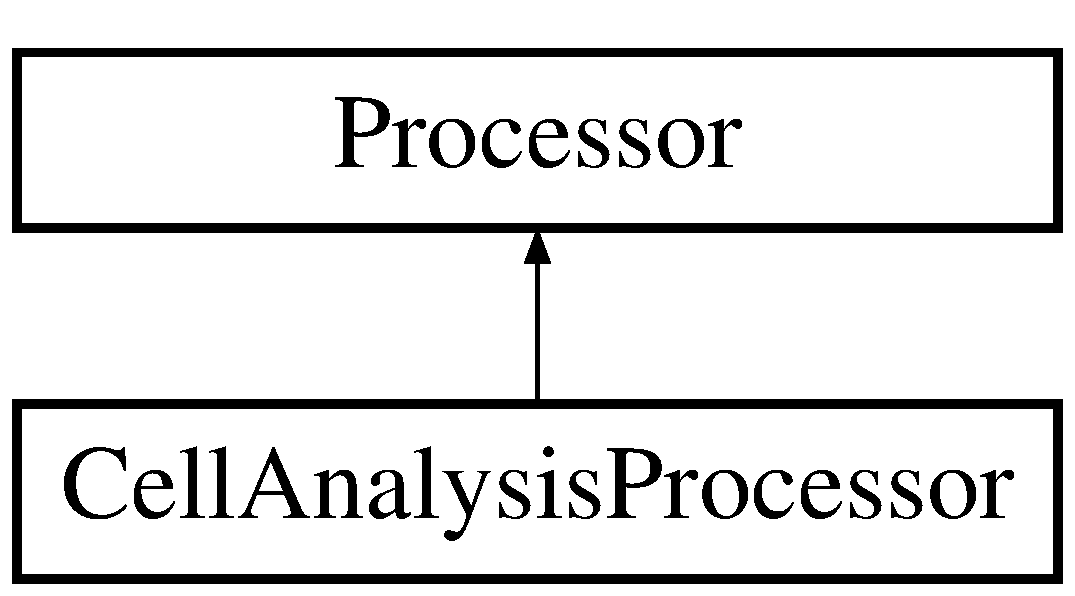
\includegraphics[height=2.000000cm]{classCellAnalysisProcessor}
\end{center}
\end{figure}
\subsection*{Public Member Functions}
\begin{DoxyCompactItemize}
\item 
{\bf Cell\-Analysis\-Processor} $\ast$ {\bfseries new\-Processor} ()\label{classCellAnalysisProcessor_a06ea545c77c9679962952e4ecc85036e}

\item 
virtual void {\bfseries init} ()\label{classCellAnalysisProcessor_a1b00ce42ce45eba2ec8837e56387fde1}

\item 
virtual void {\bfseries process\-Event} (lcio\-::\-L\-C\-Event $\ast$)\label{classCellAnalysisProcessor_ae6c3b8b71f97e13388f02abfd25ce93d}

\item 
virtual void {\bfseries end} ()\label{classCellAnalysisProcessor_a0cdbbf21c86f123832b12bf55f0c89cd}

\item 
virtual void {\bfseries open\-Input\-Collections} (lcio\-::\-L\-C\-Event $\ast$)\label{classCellAnalysisProcessor_aa3ce692d4c2f4c14653c0bebf9233b98}

\end{DoxyCompactItemize}
\subsection*{Private Member Functions}
\begin{DoxyCompactItemize}
\item 
void {\bfseries write\-Histograms} ()\label{classCellAnalysisProcessor_a25f161fbb939b83c8b6d257716cffe03}

\end{DoxyCompactItemize}
\subsection*{Private Attributes}
\begin{DoxyCompactItemize}
\item 
std\-::string {\bfseries \-\_\-input\-Muon\-Hcal\-Col\-Name}\label{classCellAnalysisProcessor_a192ef14533dd5e962c6b58f56393ed76}

\item 
std\-::string {\bfseries \-\_\-input\-Muon\-Tcmt\-Col\-Name}\label{classCellAnalysisProcessor_ae0e2834703e39e3fa9aab2007d56440e}

\item 
std\-::string {\bfseries \-\_\-rootfilename}\label{classCellAnalysisProcessor_a7cdb93f7abacb1ada4ad4ed421493e0b}

\item 
std\-::string {\bfseries \-\_\-tree\-Name}\label{classCellAnalysisProcessor_a587be2086799cd234637c08946a7499b}

\item 
std\-::string {\bfseries \-\_\-mapping\-Processor\-Name}\label{classCellAnalysisProcessor_a913b95ba8bbe5eccf8253928b50a16fe}

\item 
L\-C\-Collection $\ast$ {\bf \-\_\-tcmt\-Input\-Col}\label{classCellAnalysisProcessor_aca9af286c2a95ce17648ea2ecefed3ef}

\begin{DoxyCompactList}\small\item\em T\-C\-M\-T input collection. \end{DoxyCompactList}\item 
L\-C\-Collection $\ast$ {\bf \-\_\-hcal\-Input\-Col}\label{classCellAnalysisProcessor_a2fb10b5b1cc09ca4608868c5658279e7}

\begin{DoxyCompactList}\small\item\em H\-C\-A\-L input collection. \end{DoxyCompactList}\item 
T\-File $\ast$ {\bfseries \-\_\-rootout}\label{classCellAnalysisProcessor_a63dad02fbdf1a06166effdd1b09ba0bf}

\item 
T\-H1\-F $\ast$ {\bfseries \-\_\-tcmtenergyhistos} [M\-A\-X\-T\-C\-M\-T\-L\-A\-Y\-E\-R\-S][M\-A\-X\-T\-C\-M\-T\-S\-T\-R\-I\-P\-S]\label{classCellAnalysisProcessor_a93ffb20f66c77d0d634861972c80433a}

\item 
T\-H1\-F $\ast$ {\bfseries \-\_\-tcmtlayerenergyhistos} [M\-A\-X\-T\-C\-M\-T\-L\-A\-Y\-E\-R\-S]\label{classCellAnalysisProcessor_a171505082bf368dfe059d7c5ea636ec1}

\item 
T\-H1\-F $\ast$ {\bfseries \-\_\-hitenergyhistos} [M\-A\-X\-N\-R\-M\-O\-D\-U\-L\-E\-S][M\-A\-X\-N\-R\-C\-H\-I\-P\-S][M\-A\-X\-N\-R\-C\-H\-A\-N\-N\-E\-L\-S]\label{classCellAnalysisProcessor_abe9cc1725be61c389b70abd43791a8ef}

\item 
T\-H1\-F $\ast$ {\bfseries \-\_\-hitenergy\-Per\-Modulehistos} [M\-A\-X\-N\-R\-M\-O\-D\-U\-L\-E\-S]\label{classCellAnalysisProcessor_ac421ca529c9c5f59d9f30ae91976a19d}

\item 
T\-H1\-F $\ast$ {\bfseries \-\_\-hitenergy\-All}\label{classCellAnalysisProcessor_a9dbc72d25ba3ea61afad091824bb0d23}

\item 
T\-H1\-F $\ast$ {\bfseries \-\_\-histo\-\_\-angle}\label{classCellAnalysisProcessor_a54963d51732ca11c544d28d2b46a4481}

\item 
T\-H2\-F $\ast$ {\bfseries \-\_\-histo\-\_\-angle\-\_\-length}\label{classCellAnalysisProcessor_aae093b58b62c4bedd21d65a3d167e15e}

\item 
T\-H1\-F $\ast$ {\bfseries \-\_\-histo\-\_\-length}\label{classCellAnalysisProcessor_a98dddeb420929ad38af64a28a60464a8}

\item 
T\-H1\-F $\ast$ {\bfseries \-\_\-h\-Muon\-Hcal\-E\-Sum}\label{classCellAnalysisProcessor_a79e268c370d2149184071b1b57b5591f}

\item 
int {\bfseries \-\_\-hitenergyhistobins}\label{classCellAnalysisProcessor_a568909800005abf7c332e9e015de3da5}

\item 
float {\bfseries \-\_\-hitenergyhistomin}\label{classCellAnalysisProcessor_a948d7a77688d1ea74f84bad154af22fa}

\item 
float {\bfseries \-\_\-hitenergyhistomax}\label{classCellAnalysisProcessor_a73d5f3effdc45d019b71c73feb9ef7ad}

\item 
int {\bfseries \-\_\-calibration\-Spectra}\label{classCellAnalysisProcessor_a75de8ff1fc14d9ae09721819c3aff65d}

\item 
bool {\bfseries \-\_\-use\-T\-C\-M\-T}\label{classCellAnalysisProcessor_af0fcd0ebc329224397f66672642d7ee6}

\item 
const C\-A\-L\-I\-C\-E\-::\-Ahc\-Mapper $\ast$ {\bfseries \-\_\-ahc\-Mapper}\label{classCellAnalysisProcessor_a0cabfd5fcde81a59e8b22f55fb468f2d}

\end{DoxyCompactItemize}
\subsection*{Static Private Attributes}
\begin{DoxyCompactItemize}
\item 
static const unsigned int {\bfseries M\-A\-X\-N\-R\-M\-O\-D\-U\-L\-E\-S} = 38\label{classCellAnalysisProcessor_a2dfcec3ca068b0f9a2855d5e20985150}

\item 
static const unsigned int {\bfseries M\-A\-X\-N\-R\-C\-H\-I\-P\-S} = 12\label{classCellAnalysisProcessor_a7d6d32672684ef32a52ab06fd81a180b}

\item 
static const unsigned int {\bfseries M\-A\-X\-N\-R\-C\-H\-A\-N\-N\-E\-L\-S} = 18\label{classCellAnalysisProcessor_a40721bcdbc533caa0e84417544e7a43c}

\item 
static const unsigned int {\bfseries M\-A\-X\-T\-C\-M\-T\-L\-A\-Y\-E\-R\-S} = 16\label{classCellAnalysisProcessor_aafc3097ebf7f58966a5e5b2ec122ccba}

\item 
static const unsigned int {\bfseries M\-A\-X\-T\-C\-M\-T\-S\-T\-R\-I\-P\-S} = 20\label{classCellAnalysisProcessor_a276eab4e0cd0901968f659a727dd18a0}

\end{DoxyCompactItemize}


\subsection{Detailed Description}
Processor filling histograms for every cell identified by module, chip, channel. 

Definition at line 33 of file Cell\-Analysis\-Processor.\-hh.



The documentation for this class was generated from the following files\-:\begin{DoxyCompactItemize}
\item 
Cell\-Analysis\-Processor.\-hh\item 
Cell\-Analysis\-Processor.\-cc\end{DoxyCompactItemize}

\section{Cluster\-Ordering Class Reference}
\label{classClusterOrdering}\index{Cluster\-Ordering@{Cluster\-Ordering}}
\subsection*{Static Public Member Functions}
\begin{DoxyCompactItemize}
\item 
static bool {\bfseries compare\-Hit\-By\-Layer} (Calorimeter\-Hit $\ast$a\-Hit, Calorimeter\-Hit $\ast$b\-Hit)\label{classClusterOrdering_a98385e73ef0f15d8093401c950dc235d}

\item 
static bool {\bfseries compare\-Vect\-By\-Size} (Cluster $\ast$cluster\-A, Cluster $\ast$cluster\-B)\label{classClusterOrdering_a65fe903f58c543c843b84c2d7ee17d05}

\item 
static bool {\bfseries check\-X\-Y\-Adyacent\-Clusters} (Cluster $\ast$cluster\-A, Cluster $\ast$cluster\-B, float num\-Of\-Adyacent\-Cells)\label{classClusterOrdering_a5f63b93db02d903b457eb1a56da2d49a}

\end{DoxyCompactItemize}


\subsection{Detailed Description}


Definition at line 16 of file Cluster\-Ordering.\-hh.



The documentation for this class was generated from the following file\-:\begin{DoxyCompactItemize}
\item 
Cluster\-Ordering.\-hh\end{DoxyCompactItemize}

\section{Extract\-Intercalibration\-Processor\-:\-:condpoint Struct Reference}
\label{structExtractIntercalibrationProcessor_1_1condpoint}\index{Extract\-Intercalibration\-Processor\-::condpoint@{Extract\-Intercalibration\-Processor\-::condpoint}}
\subsection*{Data Fields}
\begin{DoxyCompactItemize}
\item 
unsigned {\bfseries vcalib}\label{structExtractIntercalibrationProcessor_1_1condpoint_ac5c276f523c1eef9621784169140e1b9}

\item 
unsigned {\bfseries shiftreg} [12]\label{structExtractIntercalibrationProcessor_1_1condpoint_ab82b62e1c2e2e4231763968305476e8c}

\end{DoxyCompactItemize}


\subsection{Detailed Description}


Definition at line 56 of file Extract\-Intercalibration\-Processor.\-hh.



The documentation for this struct was generated from the following file\-:\begin{DoxyCompactItemize}
\item 
Extract\-Intercalibration\-Processor.\-hh\end{DoxyCompactItemize}

\section{Extract\-Saturation\-Curve\-Processor\-:\-:condpoint Struct Reference}
\label{structExtractSaturationCurveProcessor_1_1condpoint}\index{Extract\-Saturation\-Curve\-Processor\-::condpoint@{Extract\-Saturation\-Curve\-Processor\-::condpoint}}
\subsection*{Data Fields}
\begin{DoxyCompactItemize}
\item 
unsigned {\bfseries vcalib}\label{structExtractSaturationCurveProcessor_1_1condpoint_a5afe22b9bd585fbb0c2c9885a131871a}

\item 
unsigned {\bfseries shiftreg} [12]\label{structExtractSaturationCurveProcessor_1_1condpoint_a228d6fdd6a981203ef981dc4f0bdd92b}

\end{DoxyCompactItemize}


\subsection{Detailed Description}


Definition at line 41 of file Extract\-Saturation\-Curve\-Processor.\-hh.



The documentation for this struct was generated from the following file\-:\begin{DoxyCompactItemize}
\item 
Extract\-Saturation\-Curve\-Processor.\-hh\end{DoxyCompactItemize}

\section{Extract\-Intercalibration\-Processor\-:\-:datapoint Struct Reference}
\label{structExtractIntercalibrationProcessor_1_1datapoint}\index{Extract\-Intercalibration\-Processor\-::datapoint@{Extract\-Intercalibration\-Processor\-::datapoint}}
\subsection*{Data Fields}
\begin{DoxyCompactItemize}
\item 
double {\bfseries sum\-Pm}\label{structExtractIntercalibrationProcessor_1_1datapoint_a2296a48fc2edf2484cea3ff63798d776}

\item 
double {\bfseries sum2\-Pm}\label{structExtractIntercalibrationProcessor_1_1datapoint_aa1bf97ae54daebe458120feb1cd20e5b}

\item 
double {\bfseries n\-Pm}\label{structExtractIntercalibrationProcessor_1_1datapoint_a2cf8aea86179310ef849273ba9aa287c}

\item 
double {\bfseries sum\-Cm}\label{structExtractIntercalibrationProcessor_1_1datapoint_a582f77796997da2d1b842f200420a5a9}

\item 
double {\bfseries sum2\-Cm}\label{structExtractIntercalibrationProcessor_1_1datapoint_aa530064426d5ddd81d516645f1a1a5b6}

\item 
double {\bfseries n\-Cm}\label{structExtractIntercalibrationProcessor_1_1datapoint_a8426e7b551c47d25856217b8d0b45579}

\end{DoxyCompactItemize}


\subsection{Detailed Description}


Definition at line 47 of file Extract\-Intercalibration\-Processor.\-hh.



The documentation for this struct was generated from the following file\-:\begin{DoxyCompactItemize}
\item 
Extract\-Intercalibration\-Processor.\-hh\end{DoxyCompactItemize}

\section{Extract\-Saturation\-Curve\-Processor\-:\-:datapoint Struct Reference}
\label{structExtractSaturationCurveProcessor_1_1datapoint}\index{Extract\-Saturation\-Curve\-Processor\-::datapoint@{Extract\-Saturation\-Curve\-Processor\-::datapoint}}
\subsection*{Data Fields}
\begin{DoxyCompactItemize}
\item 
double {\bfseries sum\-Pm}\label{structExtractSaturationCurveProcessor_1_1datapoint_a95a66cd8dc11004ee0d5bec531b6f9a3}

\item 
double {\bfseries sum2\-Pm}\label{structExtractSaturationCurveProcessor_1_1datapoint_a175a8abce00fbf18204150113b5f1dd2}

\item 
double {\bfseries n\-Pm}\label{structExtractSaturationCurveProcessor_1_1datapoint_ad6da2b245ba9533d32814a282043b131}

\item 
unsigned short {\bfseries mod\-I\-D}\label{structExtractSaturationCurveProcessor_1_1datapoint_ad82b7c88318e0150ddd4c5ef5b0246aa}

\item 
unsigned short {\bfseries cell\-K}\label{structExtractSaturationCurveProcessor_1_1datapoint_a00e2b475749c963975f90148f7e31112}

\item 
unsigned short {\bfseries no\-Over\-Adc}\label{structExtractSaturationCurveProcessor_1_1datapoint_ae299248e5420388f5c3cd72a8ca71d39}

\end{DoxyCompactItemize}


\subsection{Detailed Description}


Definition at line 32 of file Extract\-Saturation\-Curve\-Processor.\-hh.



The documentation for this struct was generated from the following file\-:\begin{DoxyCompactItemize}
\item 
Extract\-Saturation\-Curve\-Processor.\-hh\end{DoxyCompactItemize}

\section{Ecal\-Single\-Hit Struct Reference}
\label{structEcalSingleHit}\index{Ecal\-Single\-Hit@{Ecal\-Single\-Hit}}
\subsection*{Data Fields}
\begin{DoxyCompactItemize}
\item 
int {\bfseries I}\label{structEcalSingleHit_ae578cbaa0ea7c69d07c7ee4a3494b0a4}

\item 
int {\bfseries J}\label{structEcalSingleHit_added1324c391c5f65b64ff5101d57815}

\item 
int {\bfseries K}\label{structEcalSingleHit_a2b41adbb1a1951082a576e2946f2c565}

\item 
float {\bfseries x}\label{structEcalSingleHit_acbe99a6c25dbafe6c183a502d27d06fe}

\item 
float {\bfseries y}\label{structEcalSingleHit_a21bc45b5f6b8cc1d304ff8690458054c}

\item 
float {\bfseries z}\label{structEcalSingleHit_a544ae1aa36f404766d44346ba6e17bd1}

\item 
float {\bfseries energy}\label{structEcalSingleHit_abea53cadbe2e6705c61d1b31663ed6b2}

\item 
float {\bfseries hittime}\label{structEcalSingleHit_a2496240ba297d34250884676064574a2}

\item 
int {\bfseries Cell\-I\-D0}\label{structEcalSingleHit_af397ceaef3933f6572e90350a61728dd}

\item 
int {\bfseries hittype}\label{structEcalSingleHit_aec28d77ea72749051db6ddd4927aac1b}

\item 
int {\bfseries multiplicity}\label{structEcalSingleHit_a2d5b2b52900d835faed187a86c728bbe}

\item 
bool {\bfseries Overlap\-\_\-strip}\label{structEcalSingleHit_a3c05251f3b4ef3f1969de0c37de78aef}

\end{DoxyCompactItemize}


\subsection{Detailed Description}


Definition at line 4 of file Ecal\-Single\-Hits.\-hh.



The documentation for this struct was generated from the following file\-:\begin{DoxyCompactItemize}
\item 
Ecal\-Single\-Hits.\-hh\end{DoxyCompactItemize}

\section{Extract\-Intercalibration\-Processor Class Reference}
\label{classExtractIntercalibrationProcessor}\index{Extract\-Intercalibration\-Processor@{Extract\-Intercalibration\-Processor}}


Processor calculating the electronics intercalibration for each channel from a set of Pm\-Led\-Vcalib\-Scan and Cm\-Led\-Vcalib\-Scan run.  




{\ttfamily \#include $<$Extract\-Intercalibration\-Processor.\-hh$>$}

Inheritance diagram for Extract\-Intercalibration\-Processor\-:\begin{figure}[H]
\begin{center}
\leavevmode
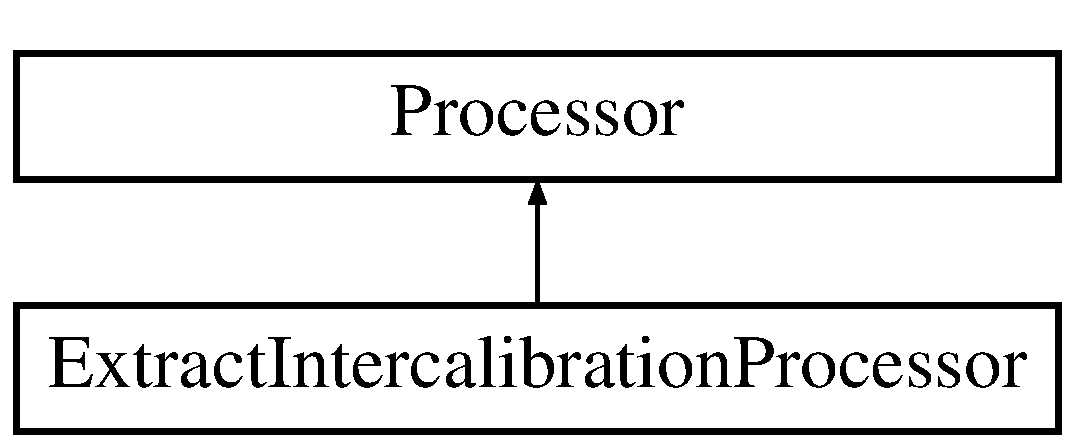
\includegraphics[height=2.000000cm]{classExtractIntercalibrationProcessor}
\end{center}
\end{figure}
\subsection*{Data Structures}
\begin{DoxyCompactItemize}
\item 
struct {\bf condpoint}
\item 
struct {\bf datapoint}
\end{DoxyCompactItemize}
\subsection*{Public Member Functions}
\begin{DoxyCompactItemize}
\item 
{\bf Extract\-Intercalibration\-Processor} $\ast$ {\bfseries new\-Processor} ()\label{classExtractIntercalibrationProcessor_af7b829330fe9a3a4700f2ff35d754c2f}

\item 
virtual void {\bfseries init} ()\label{classExtractIntercalibrationProcessor_a88dbc7b44c2dd7185efba4803f75fa6f}

\item 
void {\bfseries process\-Event} (L\-C\-Event $\ast$evt)\label{classExtractIntercalibrationProcessor_a8b9b3ce7a22525ea1fb8e56e780aa166}

\item 
virtual void {\bfseries end} ()\label{classExtractIntercalibrationProcessor_aa8cae07229f1d96ba57f17bd2aa9a9eb}

\end{DoxyCompactItemize}
\subsection*{Protected Member Functions}
\begin{DoxyCompactItemize}
\item 
void {\bfseries update\-Mapper} ()\label{classExtractIntercalibrationProcessor_a032a69f48b6fc244f50a521036c0e70f}

\end{DoxyCompactItemize}
\subsection*{Protected Attributes}
\begin{DoxyCompactItemize}
\item 
std\-::map$<$ unsigned, std\-::map\\*
$<$ unsigned, {\bf datapoint} $>$ $>$ {\bfseries \-\_\-data}\label{classExtractIntercalibrationProcessor_adf4e67f38b5b2e34e362fc2a03ed26f2}

\item 
std\-::map$<$ unsigned, {\bf condpoint} $>$ {\bfseries \-\_\-cond}\label{classExtractIntercalibrationProcessor_af577a1ce16643b016b6f8fda558f569b}

\item 
std\-::string {\bfseries \-\_\-in\-Col\-Name}\label{classExtractIntercalibrationProcessor_a19f78bf996da661aebc1b2c206e50d22}

\item 
std\-::string {\bfseries \-\_\-cond\-Col\-Name}\label{classExtractIntercalibrationProcessor_a9e1ab65990412e158f8fccd23b63bc6a}

\item 
std\-::string {\bfseries \-\_\-out\-File\-Name}\label{classExtractIntercalibrationProcessor_a40723d9a2fbb028cea27a2bf99f35109}

\item 
std\-::string {\bfseries \-\_\-mapping\-Processor\-Name}\label{classExtractIntercalibrationProcessor_a61d61974a24f4cdd95599200e6c72d24}

\item 
unsigned int {\bf \-\_\-ahc\-Max\-Number\-Of\-Chips}\label{classExtractIntercalibrationProcessor_ac5ad5bc2591002484d190cbe7c4934df}

\begin{DoxyCompactList}\small\item\em A\-H\-C\-A\-L maximum number of chips. \end{DoxyCompactList}\item 
unsigned int {\bf \-\_\-ahc\-Max\-Number\-Of\-Modules}\label{classExtractIntercalibrationProcessor_af129cc6d6cd213cbab068f478e706b94}

\begin{DoxyCompactList}\small\item\em A\-H\-C\-A\-L maximum number of modules (39) \end{DoxyCompactList}\item 
unsigned int {\bf \-\_\-ahc\-Max\-Number\-Of\-Cells}\label{classExtractIntercalibrationProcessor_a659e0f833a54e8389820d0fa6424b716}

\begin{DoxyCompactList}\small\item\em A\-H\-C\-A\-L maximum number of cells. \end{DoxyCompactList}\item 
unsigned int {\bf \-\_\-ahc\-Max\-Number\-Of\-Channels}\label{classExtractIntercalibrationProcessor_a693b0d0ebafc572ecffe39ce19b75c87}

\begin{DoxyCompactList}\small\item\em A\-H\-C\-A\-L maximum number of channels. \end{DoxyCompactList}\item 
const C\-A\-L\-I\-C\-E\-::\-Ahc\-Mapper $\ast$ {\bfseries \-\_\-ahc\-Mapper}\label{classExtractIntercalibrationProcessor_ae81b815805190b458c244c540cc4f7c8}

\item 
unsigned int {\bfseries \-\_\-mapper\-Version}\label{classExtractIntercalibrationProcessor_ac28474a6ef717635d3c79a4cb440821c}

\end{DoxyCompactItemize}


\subsection{Detailed Description}
Processor calculating the electronics intercalibration for each channel from a set of Pm\-Led\-Vcalib\-Scan and Cm\-Led\-Vcalib\-Scan run. 

At least one run of each type is needed as input files. The order is not important, the processor separates C\-M data from P\-M data.

Intercalibration factor ic = signal (C\-M) / signal (P\-M)

\begin{DoxyAuthor}{Author}
N. Meyer 
\end{DoxyAuthor}


Definition at line 29 of file Extract\-Intercalibration\-Processor.\-hh.



The documentation for this class was generated from the following files\-:\begin{DoxyCompactItemize}
\item 
Extract\-Intercalibration\-Processor.\-hh\item 
Extract\-Intercalibration\-Processor.\-cc\end{DoxyCompactItemize}

\section{Extract\-Saturation\-Curve\-Processor Class Reference}
\label{classExtractSaturationCurveProcessor}\index{Extract\-Saturation\-Curve\-Processor@{Extract\-Saturation\-Curve\-Processor}}
Inheritance diagram for Extract\-Saturation\-Curve\-Processor\-:\begin{figure}[H]
\begin{center}
\leavevmode
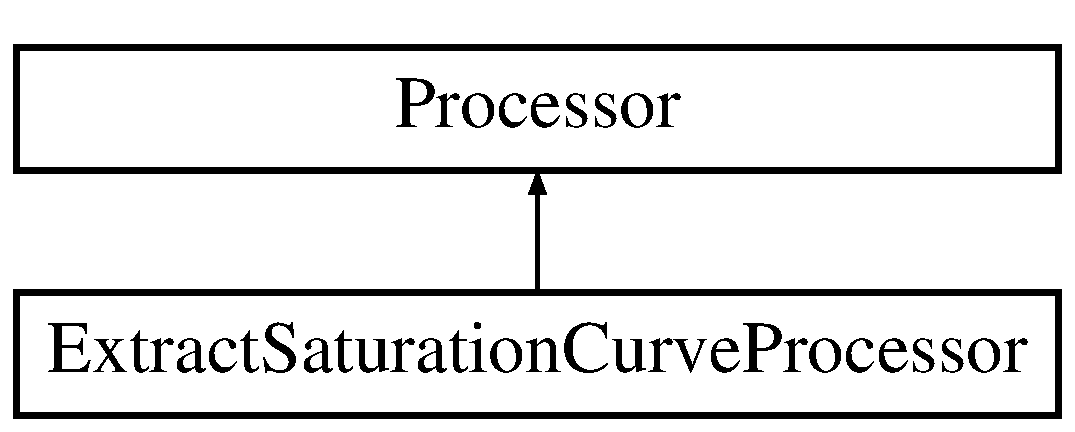
\includegraphics[height=2.000000cm]{classExtractSaturationCurveProcessor}
\end{center}
\end{figure}
\subsection*{Data Structures}
\begin{DoxyCompactItemize}
\item 
struct {\bf condpoint}
\item 
struct {\bf datapoint}
\end{DoxyCompactItemize}
\subsection*{Public Member Functions}
\begin{DoxyCompactItemize}
\item 
{\bf Extract\-Saturation\-Curve\-Processor} $\ast$ {\bfseries new\-Processor} ()\label{classExtractSaturationCurveProcessor_ac1cb6cef4f5a0a82ab72e103082a580d}

\item 
virtual void {\bfseries init} ()\label{classExtractSaturationCurveProcessor_a7feca5d6491897eb4a0642745c568049}

\item 
void {\bfseries process\-Event} (L\-C\-Event $\ast$evt)\label{classExtractSaturationCurveProcessor_a54c0e4af7a3c2c35c367035faedaf50c}

\item 
virtual void {\bfseries end} ()\label{classExtractSaturationCurveProcessor_aedeae6bf28cea73d8dbfb07307e8caa3}

\end{DoxyCompactItemize}
\subsection*{Protected Member Functions}
\begin{DoxyCompactItemize}
\item 
void {\bfseries update\-Mapper} ()\label{classExtractSaturationCurveProcessor_aae75a6b00dd5dc100b72aa560c1ee56c}

\end{DoxyCompactItemize}
\subsection*{Protected Attributes}
\begin{DoxyCompactItemize}
\item 
std\-::map$<$ unsigned, std\-::map\\*
$<$ unsigned, {\bf datapoint} $>$ $>$ {\bfseries \-\_\-data}\label{classExtractSaturationCurveProcessor_a9489d528a0de4bc27112d94c2c521e63}

\item 
std\-::map$<$ unsigned, {\bf condpoint} $>$ {\bfseries \-\_\-cond}\label{classExtractSaturationCurveProcessor_ad25bcf441fa19842d9c5c308833ba76f}

\item 
std\-::string {\bfseries \-\_\-in\-Col\-Name}\label{classExtractSaturationCurveProcessor_a50a69322210ddb62c82e3893169fa3ff}

\item 
std\-::string {\bfseries \-\_\-cond\-Col\-Name}\label{classExtractSaturationCurveProcessor_af34cd07d0d5edc67db05c9c397ac4e83}

\item 
std\-::string {\bfseries \-\_\-out\-File\-Name}\label{classExtractSaturationCurveProcessor_ab0cc84c9082e3d56fd66a84454b9a1a8}

\item 
std\-::string {\bfseries \-\_\-dat\-File\-Name}\label{classExtractSaturationCurveProcessor_aac6032684847dec6c51f8000895c906c}

\item 
bool {\bfseries \-\_\-do\-Fit}\label{classExtractSaturationCurveProcessor_a5a9f91b2696b05338c42acd717d396ec}

\item 
bool {\bfseries \-\_\-subtract\-Pedestal}\label{classExtractSaturationCurveProcessor_a81c12c771d8715003b68cdd155b93ede}

\item 
int {\bfseries \-\_\-n\-Points\-Used}\label{classExtractSaturationCurveProcessor_a83bcac5b9e763bc07522c99028dc4da3}

\item 
int {\bfseries \-\_\-led\-Type}\label{classExtractSaturationCurveProcessor_a788ccfcf2d60cdd98fa58b8a25960870}

\item 
unsigned int {\bfseries vcell}\label{classExtractSaturationCurveProcessor_a6b92dcd2b25a6e15a9c5e54c964c448a}

\item 
unsigned int {\bf \-\_\-ahc\-Max\-Number\-Of\-Chips}\label{classExtractSaturationCurveProcessor_a6504d810d836fce199cb3a0672c0e7b8}

\begin{DoxyCompactList}\small\item\em A\-H\-C\-A\-L maximum number of chips. \end{DoxyCompactList}\item 
unsigned int {\bf \-\_\-ahc\-Max\-Number\-Of\-Modules}\label{classExtractSaturationCurveProcessor_a27dadca929860032628e9e5984c4635b}

\begin{DoxyCompactList}\small\item\em A\-H\-C\-A\-L maximum number of modules (39) \end{DoxyCompactList}\item 
unsigned int {\bf \-\_\-ahc\-Max\-Number\-Of\-Cells}\label{classExtractSaturationCurveProcessor_a78254103bebe4692ff7113e20be44381}

\begin{DoxyCompactList}\small\item\em A\-H\-C\-A\-L maximum number of cells. \end{DoxyCompactList}\item 
unsigned int {\bf \-\_\-ahc\-Max\-Number\-Of\-Channels}\label{classExtractSaturationCurveProcessor_ab4e53af430d5dd5ccf667a4d3f3c2176}

\begin{DoxyCompactList}\small\item\em A\-H\-C\-A\-L maximum number of channels. \end{DoxyCompactList}\item 
const C\-A\-L\-I\-C\-E\-::\-Ahc\-Mapper $\ast$ {\bfseries \-\_\-ahc\-Mapper}\label{classExtractSaturationCurveProcessor_aad14e61b12d09a38bdbb0128ea8dc2c8}

\item 
unsigned int {\bfseries \-\_\-mapper\-Version}\label{classExtractSaturationCurveProcessor_ae74dd1f33b1ff0ae67e32384bd33d0bf}

\item 
std\-::string {\bfseries \-\_\-mapping\-Processor\-Name}\label{classExtractSaturationCurveProcessor_a46e5e0f8be8ef1842cd478b8be63558c}

\end{DoxyCompactItemize}


\subsection{Detailed Description}


Definition at line 14 of file Extract\-Saturation\-Curve\-Processor.\-hh.



The documentation for this class was generated from the following files\-:\begin{DoxyCompactItemize}
\item 
Extract\-Saturation\-Curve\-Processor.\-hh\item 
Extract\-Saturation\-Curve\-Processor.\-cc\end{DoxyCompactItemize}

\section{Hcal\-Single\-Hit Struct Reference}
\label{structHcalSingleHit}\index{Hcal\-Single\-Hit@{Hcal\-Single\-Hit}}
\subsection*{Data Fields}
\begin{DoxyCompactItemize}
\item 
int {\bfseries I}\label{structHcalSingleHit_ab8c785a4cf4d343ad7e107cbb4ef737d}

\item 
int {\bfseries J}\label{structHcalSingleHit_a28f963e1b6afb63f68b824edf25e171b}

\item 
int {\bfseries K}\label{structHcalSingleHit_acaae346035a5bf06db83b34f0dd794b4}

\item 
float {\bfseries x}\label{structHcalSingleHit_ad7efe549fc3d0edf935f0eff913ab715}

\item 
float {\bfseries y}\label{structHcalSingleHit_a1f42473073dc1eedc9c356118580f8da}

\item 
float {\bfseries z}\label{structHcalSingleHit_a64a006c07bf06ce1fee5666630cfd6d7}

\item 
float {\bfseries energy}\label{structHcalSingleHit_a42b6143ec67442d89723416d5172f868}

\item 
float {\bfseries hittime}\label{structHcalSingleHit_a52d543104083887e9c44257fe4b6b956}

\item 
int {\bfseries hittype}\label{structHcalSingleHit_a09d33f63cd72d0ac0e137d0c0cda298e}

\item 
int {\bfseries Cell\-I\-D0}\label{structHcalSingleHit_aec5d1fcebcf983054bb4de6ae5ba79f8}

\end{DoxyCompactItemize}


\subsection{Detailed Description}


Definition at line 4 of file Hcal\-Single\-Hits.\-hh.



The documentation for this struct was generated from the following file\-:\begin{DoxyCompactItemize}
\item 
Hcal\-Single\-Hits.\-hh\end{DoxyCompactItemize}

\section{C\-A\-L\-I\-C\-E\-:\-:Ahc2\-Time\-Calibrator\-:\-:Hit Struct Reference}
\label{structCALICE_1_1Ahc2TimeCalibrator_1_1Hit}\index{C\-A\-L\-I\-C\-E\-::\-Ahc2\-Time\-Calibrator\-::\-Hit@{C\-A\-L\-I\-C\-E\-::\-Ahc2\-Time\-Calibrator\-::\-Hit}}
\subsection*{Data Fields}
\begin{DoxyCompactItemize}
\item 
int {\bfseries B\-X\-I\-D} = 0\label{structCALICE_1_1Ahc2TimeCalibrator_1_1Hit_a9521ee5cc3f451e8ce252c2addbdec03}

\item 
int {\bfseries Memory\-Cell} = 0\label{structCALICE_1_1Ahc2TimeCalibrator_1_1Hit_aec3957052ebe5abc3bf90773ead2a4ae}

\item 
int {\bfseries Cycle\-Nr} = 0\label{structCALICE_1_1Ahc2TimeCalibrator_1_1Hit_a3647da8c2def0b2c03a6e6823b9007fa}

\item 
int {\bfseries Hit\-Bit} = 0\label{structCALICE_1_1Ahc2TimeCalibrator_1_1Hit_ad29f4d2d6bf77c12787c3c86f327d845}

\item 
int {\bfseries Gain\-Bit} = 0\label{structCALICE_1_1Ahc2TimeCalibrator_1_1Hit_a191d6c07f9d573e88b768e5cd595db97}

\item 
int {\bfseries Module\-Nr} = 0\label{structCALICE_1_1Ahc2TimeCalibrator_1_1Hit_ae12e9fee470de9daba04f7cbc3b8adf4}

\item 
int {\bfseries Chip\-Nr} = 0\label{structCALICE_1_1Ahc2TimeCalibrator_1_1Hit_a861b9551dbc98786e610e683b464eb3e}

\item 
int {\bfseries Chip\-I\-D} = 0\label{structCALICE_1_1Ahc2TimeCalibrator_1_1Hit_a11861aac201c338f419ce6a05715d5b6}

\item 
int {\bfseries Module\-I\-D} = 0\label{structCALICE_1_1Ahc2TimeCalibrator_1_1Hit_a1fb8417d12cca4344f321074cbff7e23}

\item 
int {\bfseries Channel} = 0\label{structCALICE_1_1Ahc2TimeCalibrator_1_1Hit_aa704b776ce45270395e7ed927437ea77}

\item 
short {\bfseries A\-D\-C} = 0\label{structCALICE_1_1Ahc2TimeCalibrator_1_1Hit_a575fab6e6f3602f2af86fb0b19a66053}

\item 
short {\bfseries T\-D\-C} = 0\label{structCALICE_1_1Ahc2TimeCalibrator_1_1Hit_a47e2321bfb9be5e31190eb33cdc36bf0}

\item 
float {\bfseries time\-Reference} = 0\label{structCALICE_1_1Ahc2TimeCalibrator_1_1Hit_a1fbab4ea5c88f0e50f7c943fd69e0390}

\end{DoxyCompactItemize}


\subsection{Detailed Description}


Definition at line 65 of file Ahc2\-Time\-Calibrator.\-hh.



The documentation for this struct was generated from the following file\-:\begin{DoxyCompactItemize}
\item 
Ahc2\-Time\-Calibrator.\-hh\end{DoxyCompactItemize}

\section{C\-A\-L\-I\-C\-E\-:\-:Mip\-Track\-Finder Class Reference}
\label{classCALICE_1_1MipTrackFinder}\index{C\-A\-L\-I\-C\-E\-::\-Mip\-Track\-Finder@{C\-A\-L\-I\-C\-E\-::\-Mip\-Track\-Finder}}


Processor to extract M\-I\-P calibrations from muon beam runs.  




{\ttfamily \#include $<$Mip\-Track\-Finder.\-hh$>$}

Inheritance diagram for C\-A\-L\-I\-C\-E\-:\-:Mip\-Track\-Finder\-:\begin{figure}[H]
\begin{center}
\leavevmode
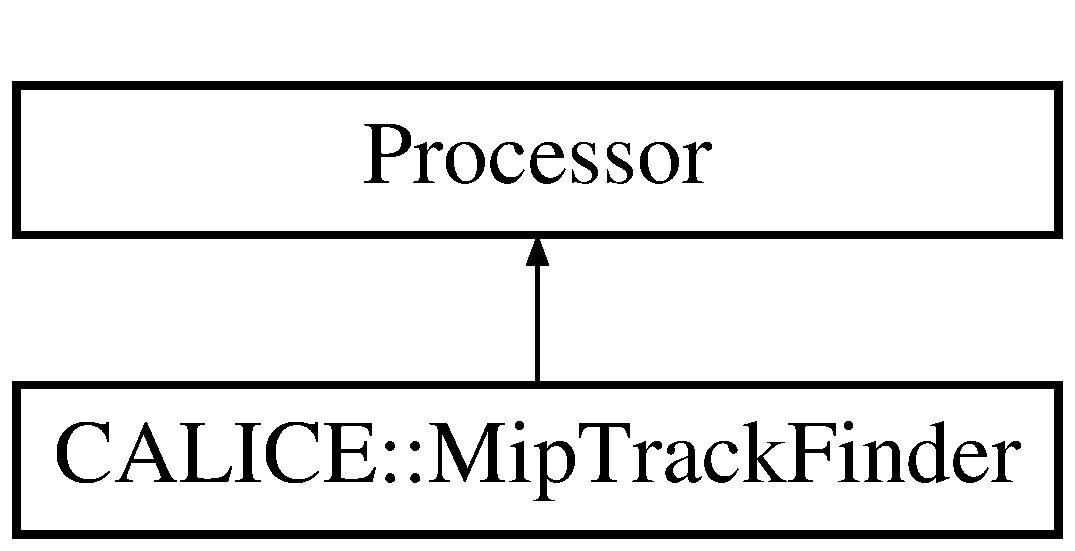
\includegraphics[height=2.000000cm]{classCALICE_1_1MipTrackFinder}
\end{center}
\end{figure}
\subsection*{Public Member Functions}
\begin{DoxyCompactItemize}
\item 
virtual Processor $\ast$ {\bf new\-Processor} ()\label{classCALICE_1_1MipTrackFinder_a55a7f624a6bb8628c8e8516976593d71}

\begin{DoxyCompactList}\small\item\em Return new instance of this processor. \end{DoxyCompactList}\item 
{\bf Mip\-Track\-Finder} ()\label{classCALICE_1_1MipTrackFinder_a3806b8a42dbf92ec4ed61c1c8a8fbb94}

\begin{DoxyCompactList}\small\item\em Default constructor. \end{DoxyCompactList}\item 
{\bf $\sim$\-Mip\-Track\-Finder} ()\label{classCALICE_1_1MipTrackFinder_ae52b812fd15b89fd36954dcea97b4cf2}

\begin{DoxyCompactList}\small\item\em Destructor. \end{DoxyCompactList}\item 
virtual void {\bf init} ()\label{classCALICE_1_1MipTrackFinder_a99b9bed4ba17213c6b267bfbdc0ad9ce}

\begin{DoxyCompactList}\small\item\em Initialise useful variables. \end{DoxyCompactList}\item 
virtual void {\bf process\-Event} (L\-C\-Event $\ast$evt)
\begin{DoxyCompactList}\small\item\em Process event (the working horse) \end{DoxyCompactList}\item 
virtual void {\bf end} ()\label{classCALICE_1_1MipTrackFinder_ab580d34d2e630152123a1af2e24db24a}

\begin{DoxyCompactList}\small\item\em Function to be called at the end of the job, after all events have been processed, for clean up. \end{DoxyCompactList}\end{DoxyCompactItemize}
\subsection*{Private Member Functions}
\begin{DoxyCompactItemize}
\item 
void {\bf open\-Input\-Collections} (L\-C\-Event $\ast$evt)
\begin{DoxyCompactList}\small\item\em Open the input collections. \end{DoxyCompactList}\item 
void {\bf find\-Track} (L\-C\-Event $\ast$evt)
\begin{DoxyCompactList}\small\item\em Find the track. \end{DoxyCompactList}\item 
bool {\bf do\-Further\-Analysis} ()
\begin{DoxyCompactList}\small\item\em Check if cuts are fullfilled, and if analysis is to be continued. \end{DoxyCompactList}\item 
L\-C\-Typed\-Vector$<$ Calorimeter\-Hit $>$ $\ast$ {\bf extract\-A\-H\-C\-A\-L\-Information} ()\label{classCALICE_1_1MipTrackFinder_a32af780e878464a7fe59b641610cc8e6}

\begin{DoxyCompactList}\small\item\em Extract A\-H\-C\-A\-L information. \end{DoxyCompactList}\item 
std\-::pair$<$ int, float $>$ {\bf extract\-Number\-Of\-Hits\-And\-Energy\-Sum} (L\-C\-Collection $\ast$input\-Col)
\begin{DoxyCompactList}\small\item\em Extract number of hits and the energy sum from the input collection. \end{DoxyCompactList}\item 
E\-V\-E\-N\-T\-::\-Cluster\-Vec {\bf find\-Track\-Clusters} (L\-C\-Typed\-Vector$<$ Calorimeter\-Hit $>$ $\ast$hcal\-Vec)
\begin{DoxyCompactList}\small\item\em Find clusters of M\-I\-P tracks. \end{DoxyCompactList}\item 
E\-V\-E\-N\-T\-::\-Cluster\-Vec {\bf select\-Track\-Clusters} (E\-V\-E\-N\-T\-::\-Cluster\-Vec cluster\-Vec, const std\-::string track\-Selection\-Mode)
\begin{DoxyCompactList}\small\item\em Select good tracks. \end{DoxyCompactList}\item 
Cluster\-Impl $\ast$ {\bf get\-Whole\-Track} (Cluster $\ast$track\-Cluster)
\begin{DoxyCompactList}\small\item\em Get the whole track (i.\-e. \end{DoxyCompactList}\item 
E\-V\-E\-N\-T\-::\-Cluster\-Vec {\bf get\-Remaining\-Hits} (E\-V\-E\-N\-T\-::\-Cluster\-Vec selected\-Track\-Clusters)
\begin{DoxyCompactList}\small\item\em Get the vector of track clusters containing all the remaining hits. \end{DoxyCompactList}\item 
void {\bf append\-Parameters} (L\-C\-Event $\ast$evt, E\-V\-E\-N\-T\-::\-Cluster\-Vec final\-Vec)
\begin{DoxyCompactList}\small\item\em Append event parameters with basic track information. \end{DoxyCompactList}\item 
void {\bf create\-Output\-Collection} (L\-C\-Event $\ast$evt, E\-V\-E\-N\-T\-::\-Cluster\-Vec final\-Vec)
\begin{DoxyCompactList}\small\item\em Create output collection of track clusters. \end{DoxyCompactList}\end{DoxyCompactItemize}
\subsection*{Private Attributes}
\begin{DoxyCompactItemize}
\item 
const Mapper $\ast$ {\bf \-\_\-mapper}\label{classCALICE_1_1MipTrackFinder_af8ea6a3ae97f2df24592e914ff613203}

\begin{DoxyCompactList}\small\item\em the mapper \end{DoxyCompactList}\item 
std\-::string {\bf \-\_\-mapping\-Processor\-Name}\label{classCALICE_1_1MipTrackFinder_a19a0560f8d46d6669b10f253f21f6e7a}

\begin{DoxyCompactList}\small\item\em name of the processor which provides the mapping \end{DoxyCompactList}\item 
std\-::string {\bf \-\_\-cell\-Description\-Processor\-Name}\label{classCALICE_1_1MipTrackFinder_a6df4ecb6db21429aefd2900cdc1e4fb7}

\begin{DoxyCompactList}\small\item\em name of the processor which provides the cells description \end{DoxyCompactList}\item 
Mapped\-Container\\*
$<$ C\-A\-L\-I\-C\-E\-::\-Cell\-Description $>$ $\ast$ {\bf \-\_\-cell\-Descriptions}\label{classCALICE_1_1MipTrackFinder_aefbda6dfe51dc6bcfc5c1e33da66f9cc}

\begin{DoxyCompactList}\small\item\em mapped container of cells description \end{DoxyCompactList}\item 
L\-C\-Collection $\ast$ {\bf \-\_\-ecal\-Input\-Col}\label{classCALICE_1_1MipTrackFinder_aad63fbdc5a30192ec5cf167513b9ad42}

\begin{DoxyCompactList}\small\item\em E\-C\-A\-L input collection. \end{DoxyCompactList}\item 
L\-C\-Collection $\ast$ {\bf \-\_\-ahcal\-Input\-Col}\label{classCALICE_1_1MipTrackFinder_a0d088912057e75d9f714e10618e45a64}

\begin{DoxyCompactList}\small\item\em A\-H\-C\-A\-L input collection. \end{DoxyCompactList}\item 
L\-C\-Collection $\ast$ {\bf \-\_\-ahcal\-Amp\-Input\-Col}\label{classCALICE_1_1MipTrackFinder_a60d1306464699c01c609abc7f8edddaa}

\begin{DoxyCompactList}\small\item\em A\-H\-C\-A\-L Amplitude input collection. \end{DoxyCompactList}\item 
L\-C\-Collection $\ast$ {\bf \-\_\-tcmt\-Input\-Col}\label{classCALICE_1_1MipTrackFinder_a3e4410c59519f6a9ba69aa07983ebeb0}

\begin{DoxyCompactList}\small\item\em T\-C\-M\-T input collection. \end{DoxyCompactList}\item 
std\-::string {\bfseries \-\_\-ecal\-Input\-Col\-Name}\label{classCALICE_1_1MipTrackFinder_aede8ca5f1ff5926b465b427f1e4f9a97}

\item 
std\-::string {\bfseries \-\_\-ahcal\-Input\-Col\-Name}\label{classCALICE_1_1MipTrackFinder_ae71300eb7bcb4d10522c49cba491b995}

\item 
std\-::string {\bfseries \-\_\-ahcal\-Amp\-Input\-Col\-Name}\label{classCALICE_1_1MipTrackFinder_a2e88acac7e2cfa5be020b3fbe9448442}

\item 
std\-::string {\bfseries \-\_\-ahcal\-Output\-Track\-Col\-Name}\label{classCALICE_1_1MipTrackFinder_a514a9e8135b991d26fda0df6cb4e5740}

\item 
std\-::string {\bfseries \-\_\-tcmt\-Input\-Col\-Name}\label{classCALICE_1_1MipTrackFinder_a4f087086c49cb3721e512d68c1eac320}

\item 
std\-::string {\bf \-\_\-track\-Selection\-Mode}\label{classCALICE_1_1MipTrackFinder_a6e6e7284cd571e5c093b69ee1a253ae7}

\begin{DoxyCompactList}\small\item\em track selection mode\-: N\-H\-I\-Ts = based on the number of hits; P\-E\-R\-P\-E\-N\-D\-I\-C\-U\-L\-A\-R = select only perpendicular tracks \end{DoxyCompactList}\item 
bool {\bf \-\_\-use\-E\-C\-A\-Land\-T\-C\-M\-T}\label{classCALICE_1_1MipTrackFinder_ab0c70fcc6c54979eb0a24466fc667912}

\begin{DoxyCompactList}\small\item\em decide whether to use E\-C\-A\-L and T\-C\-M\-T input information (default\-: false) \end{DoxyCompactList}\item 
bool {\bf \-\_\-is\-Non\-Muon\-Run}\label{classCALICE_1_1MipTrackFinder_a9e36ce713512208024f7e677f24d70fb}

\begin{DoxyCompactList}\small\item\em flag for non-\/muon run \end{DoxyCompactList}\item 
int {\bf \-\_\-ahcal\-Max\-No\-Hits}\label{classCALICE_1_1MipTrackFinder_a91d061c42a10457d8e24b90cd298e634}

\begin{DoxyCompactList}\small\item\em maximum number of hits in the A\-H\-C\-A\-L \end{DoxyCompactList}\item 
int {\bf \-\_\-ecal\-Min\-No\-Hits}\label{classCALICE_1_1MipTrackFinder_aa7b08125cf046d630365de5f55cfbb6b}

\begin{DoxyCompactList}\small\item\em minimum number of hits in the E\-C\-A\-L \end{DoxyCompactList}\item 
int {\bf \-\_\-ecal\-Max\-No\-Hits}\label{classCALICE_1_1MipTrackFinder_ad02eebf5cf6fef77436863f907374423}

\begin{DoxyCompactList}\small\item\em maximum number of hits in the E\-C\-A\-L \end{DoxyCompactList}\item 
float {\bf \-\_\-tcmt\-Min\-Energy\-Sum}\label{classCALICE_1_1MipTrackFinder_af0a0a7decf81c16e7cfc8eab31e67a77}

\begin{DoxyCompactList}\small\item\em minimum energy sum in the T\-C\-M\-T \end{DoxyCompactList}\item 
float {\bf \-\_\-mip\-Cut\-Value}\label{classCALICE_1_1MipTrackFinder_a64adc19b661b41b9867c5c56f247778d}

\begin{DoxyCompactList}\small\item\em M\-I\-P cut value (0.\-5 M\-I\-Ps) \end{DoxyCompactList}\item 
int {\bfseries \-\_\-mip\-Cut\-Variable}\label{classCALICE_1_1MipTrackFinder_a19e45f827fa9c2b8f52ab7dc42fffd96}

\item 
int {\bf \-\_\-track\-No\-Hits\-Threshold}
\begin{DoxyCompactList}\small\item\em choose amplitude to be used to perform the mip cut \end{DoxyCompactList}\item 
Int\-Vec {\bf \-\_\-bad\-Ahcal\-Modules\-Vec}\label{classCALICE_1_1MipTrackFinder_acd8b079f861742d25cc2fcfc6ccfb763}

\begin{DoxyCompactList}\small\item\em vector of bad A\-H\-C\-A\-L modules numbers \end{DoxyCompactList}\item 
Int\-Vec {\bf \-\_\-first\-Ahcal\-Modules\-Vec}\label{classCALICE_1_1MipTrackFinder_adc6d58d6ee59a8530f1a6439bd02ae3d}

\begin{DoxyCompactList}\small\item\em vector of numbers of the beginning A\-H\-C\-A\-L modules which are used for perpendicular track finding \end{DoxyCompactList}\item 
Int\-Vec {\bf \-\_\-last\-Ahcal\-Modules\-Vec}\label{classCALICE_1_1MipTrackFinder_a08397bf4269e486cc906a645b26f5a7c}

\begin{DoxyCompactList}\small\item\em vector of numbers of the ending A\-H\-C\-A\-L modules which are used for perpendicular track finding \end{DoxyCompactList}\item 
E\-V\-E\-N\-T\-::\-Calorimeter\-Hit\-Vec {\bf \-\_\-all\-Ahcal\-Hits\-In\-Event\-Vec}\label{classCALICE_1_1MipTrackFinder_a4c48ff185ec8093624934b9c023d2057}

\begin{DoxyCompactList}\small\item\em vector containing all A\-H\-C\-A\-L hits from the event \end{DoxyCompactList}\end{DoxyCompactItemize}


\subsection{Detailed Description}
Processor to extract M\-I\-P calibrations from muon beam runs. 

\begin{DoxyAuthor}{Author}
N.\-D'Ascenzo, D\-E\-S\-Y, S. Richter, D\-E\-S\-Y 
\end{DoxyAuthor}
\begin{DoxyDate}{Date}
Jul 13 2006, 2008 
\end{DoxyDate}


Definition at line 27 of file Mip\-Track\-Finder.\-hh.



\subsection{Member Function Documentation}
\index{C\-A\-L\-I\-C\-E\-::\-Mip\-Track\-Finder@{C\-A\-L\-I\-C\-E\-::\-Mip\-Track\-Finder}!append\-Parameters@{append\-Parameters}}
\index{append\-Parameters@{append\-Parameters}!CALICE::MipTrackFinder@{C\-A\-L\-I\-C\-E\-::\-Mip\-Track\-Finder}}
\subsubsection[{append\-Parameters}]{\setlength{\rightskip}{0pt plus 5cm}void C\-A\-L\-I\-C\-E\-::\-Mip\-Track\-Finder\-::append\-Parameters (
\begin{DoxyParamCaption}
\item[{L\-C\-Event $\ast$}]{evt, }
\item[{E\-V\-E\-N\-T\-::\-Cluster\-Vec}]{final\-Vec}
\end{DoxyParamCaption}
)\hspace{0.3cm}{\ttfamily [private]}}\label{classCALICE_1_1MipTrackFinder_afed445ffc703d8aab42b72f8caea22f5}


Append event parameters with basic track information. 


\begin{DoxyParams}{Parameters}
{\em evt} & the processed event \\
\hline
{\em final\-Vec} & final vector of track clusters, after all selections \\
\hline
\end{DoxyParams}


Definition at line 674 of file Mip\-Track\-Finder.\-cc.



Referenced by find\-Track().

\index{C\-A\-L\-I\-C\-E\-::\-Mip\-Track\-Finder@{C\-A\-L\-I\-C\-E\-::\-Mip\-Track\-Finder}!create\-Output\-Collection@{create\-Output\-Collection}}
\index{create\-Output\-Collection@{create\-Output\-Collection}!CALICE::MipTrackFinder@{C\-A\-L\-I\-C\-E\-::\-Mip\-Track\-Finder}}
\subsubsection[{create\-Output\-Collection}]{\setlength{\rightskip}{0pt plus 5cm}void C\-A\-L\-I\-C\-E\-::\-Mip\-Track\-Finder\-::create\-Output\-Collection (
\begin{DoxyParamCaption}
\item[{L\-C\-Event $\ast$}]{evt, }
\item[{E\-V\-E\-N\-T\-::\-Cluster\-Vec}]{final\-Vec}
\end{DoxyParamCaption}
)\hspace{0.3cm}{\ttfamily [private]}}\label{classCALICE_1_1MipTrackFinder_a9c4c925f38c5746f61e0b0709f05c03a}


Create output collection of track clusters. 


\begin{DoxyParams}{Parameters}
{\em evt} & the processed event \\
\hline
{\em final\-Vec} & final vector of track clusters, after all selections \\
\hline
\end{DoxyParams}


Definition at line 702 of file Mip\-Track\-Finder.\-cc.



Referenced by find\-Track().

\index{C\-A\-L\-I\-C\-E\-::\-Mip\-Track\-Finder@{C\-A\-L\-I\-C\-E\-::\-Mip\-Track\-Finder}!do\-Further\-Analysis@{do\-Further\-Analysis}}
\index{do\-Further\-Analysis@{do\-Further\-Analysis}!CALICE::MipTrackFinder@{C\-A\-L\-I\-C\-E\-::\-Mip\-Track\-Finder}}
\subsubsection[{do\-Further\-Analysis}]{\setlength{\rightskip}{0pt plus 5cm}bool C\-A\-L\-I\-C\-E\-::\-Mip\-Track\-Finder\-::do\-Further\-Analysis (
\begin{DoxyParamCaption}
{}
\end{DoxyParamCaption}
)\hspace{0.3cm}{\ttfamily [private]}}\label{classCALICE_1_1MipTrackFinder_aab79ba892b9cacc87b2d2983bb859606}


Check if cuts are fullfilled, and if analysis is to be continued. 

\begin{DoxyReturn}{Returns}
analyse flag to show if the cuts are fullfilled or not 
\end{DoxyReturn}


Definition at line 276 of file Mip\-Track\-Finder.\-cc.



References \-\_\-ahcal\-Input\-Col, \-\_\-ahcal\-Max\-No\-Hits, \-\_\-ecal\-Input\-Col, \-\_\-ecal\-Max\-No\-Hits, \-\_\-ecal\-Min\-No\-Hits, \-\_\-is\-Non\-Muon\-Run, \-\_\-tcmt\-Input\-Col, \-\_\-tcmt\-Min\-Energy\-Sum, \-\_\-use\-E\-C\-A\-Land\-T\-C\-M\-T, and extract\-Number\-Of\-Hits\-And\-Energy\-Sum().



Referenced by find\-Track().

\index{C\-A\-L\-I\-C\-E\-::\-Mip\-Track\-Finder@{C\-A\-L\-I\-C\-E\-::\-Mip\-Track\-Finder}!extract\-Number\-Of\-Hits\-And\-Energy\-Sum@{extract\-Number\-Of\-Hits\-And\-Energy\-Sum}}
\index{extract\-Number\-Of\-Hits\-And\-Energy\-Sum@{extract\-Number\-Of\-Hits\-And\-Energy\-Sum}!CALICE::MipTrackFinder@{C\-A\-L\-I\-C\-E\-::\-Mip\-Track\-Finder}}
\subsubsection[{extract\-Number\-Of\-Hits\-And\-Energy\-Sum}]{\setlength{\rightskip}{0pt plus 5cm}std\-::pair$<$ int, float $>$ C\-A\-L\-I\-C\-E\-::\-Mip\-Track\-Finder\-::extract\-Number\-Of\-Hits\-And\-Energy\-Sum (
\begin{DoxyParamCaption}
\item[{L\-C\-Collection $\ast$}]{input\-Col}
\end{DoxyParamCaption}
)\hspace{0.3cm}{\ttfamily [private]}}\label{classCALICE_1_1MipTrackFinder_a1aef1a8fd625a33ec44d91dab476b45c}


Extract number of hits and the energy sum from the input collection. 


\begin{DoxyParams}{Parameters}
{\em input\-Col} & the input collection \\
\hline
\end{DoxyParams}


Definition at line 342 of file Mip\-Track\-Finder.\-cc.



Referenced by do\-Further\-Analysis().

\index{C\-A\-L\-I\-C\-E\-::\-Mip\-Track\-Finder@{C\-A\-L\-I\-C\-E\-::\-Mip\-Track\-Finder}!find\-Track@{find\-Track}}
\index{find\-Track@{find\-Track}!CALICE::MipTrackFinder@{C\-A\-L\-I\-C\-E\-::\-Mip\-Track\-Finder}}
\subsubsection[{find\-Track}]{\setlength{\rightskip}{0pt plus 5cm}void C\-A\-L\-I\-C\-E\-::\-Mip\-Track\-Finder\-::find\-Track (
\begin{DoxyParamCaption}
\item[{L\-C\-Event $\ast$}]{evt}
\end{DoxyParamCaption}
)\hspace{0.3cm}{\ttfamily [private]}}\label{classCALICE_1_1MipTrackFinder_ab02037fc2a5b5bc03cc9c0a009705cf0}


Find the track. 


\begin{DoxyParams}{Parameters}
{\em evt} & event to be processed \\
\hline
\end{DoxyParams}


Definition at line 230 of file Mip\-Track\-Finder.\-cc.



References \-\_\-track\-Selection\-Mode, append\-Parameters(), create\-Output\-Collection(), do\-Further\-Analysis(), extract\-A\-H\-C\-A\-L\-Information(), find\-Track\-Clusters(), get\-Remaining\-Hits(), and select\-Track\-Clusters().



Referenced by process\-Event().

\index{C\-A\-L\-I\-C\-E\-::\-Mip\-Track\-Finder@{C\-A\-L\-I\-C\-E\-::\-Mip\-Track\-Finder}!find\-Track\-Clusters@{find\-Track\-Clusters}}
\index{find\-Track\-Clusters@{find\-Track\-Clusters}!CALICE::MipTrackFinder@{C\-A\-L\-I\-C\-E\-::\-Mip\-Track\-Finder}}
\subsubsection[{find\-Track\-Clusters}]{\setlength{\rightskip}{0pt plus 5cm}E\-V\-E\-N\-T\-::\-Cluster\-Vec C\-A\-L\-I\-C\-E\-::\-Mip\-Track\-Finder\-::find\-Track\-Clusters (
\begin{DoxyParamCaption}
\item[{L\-C\-Typed\-Vector$<$ Calorimeter\-Hit $>$ $\ast$}]{hcal\-Vec}
\end{DoxyParamCaption}
)\hspace{0.3cm}{\ttfamily [private]}}\label{classCALICE_1_1MipTrackFinder_a2fcd9079e5fca39cf6eb91f6a2a59f72}


Find clusters of M\-I\-P tracks. 


\begin{DoxyParams}{Parameters}
{\em hcal\-Vec} & input vector of A\-H\-C\-A\-L hits \\
\hline
\end{DoxyParams}
\begin{DoxyReturn}{Returns}
vector of clusters 
\end{DoxyReturn}


Definition at line 465 of file Mip\-Track\-Finder.\-cc.



References \-\_\-cell\-Descriptions, and \-\_\-mapper.



Referenced by find\-Track().

\index{C\-A\-L\-I\-C\-E\-::\-Mip\-Track\-Finder@{C\-A\-L\-I\-C\-E\-::\-Mip\-Track\-Finder}!get\-Remaining\-Hits@{get\-Remaining\-Hits}}
\index{get\-Remaining\-Hits@{get\-Remaining\-Hits}!CALICE::MipTrackFinder@{C\-A\-L\-I\-C\-E\-::\-Mip\-Track\-Finder}}
\subsubsection[{get\-Remaining\-Hits}]{\setlength{\rightskip}{0pt plus 5cm}E\-V\-E\-N\-T\-::\-Cluster\-Vec C\-A\-L\-I\-C\-E\-::\-Mip\-Track\-Finder\-::get\-Remaining\-Hits (
\begin{DoxyParamCaption}
\item[{E\-V\-E\-N\-T\-::\-Cluster\-Vec}]{selected\-Track\-Clusters}
\end{DoxyParamCaption}
)\hspace{0.3cm}{\ttfamily [private]}}\label{classCALICE_1_1MipTrackFinder_a7ef668cb721bb6efe876222827fb7052}


Get the vector of track clusters containing all the remaining hits. 


\begin{DoxyParams}{Parameters}
{\em selected\-Track\-Clusters} & vector of selected track clusters \\
\hline
\end{DoxyParams}
\begin{DoxyReturn}{Returns}
vector of track clusters containing all the remaining hits 
\end{DoxyReturn}


Definition at line 658 of file Mip\-Track\-Finder.\-cc.



References get\-Whole\-Track().



Referenced by find\-Track().

\index{C\-A\-L\-I\-C\-E\-::\-Mip\-Track\-Finder@{C\-A\-L\-I\-C\-E\-::\-Mip\-Track\-Finder}!get\-Whole\-Track@{get\-Whole\-Track}}
\index{get\-Whole\-Track@{get\-Whole\-Track}!CALICE::MipTrackFinder@{C\-A\-L\-I\-C\-E\-::\-Mip\-Track\-Finder}}
\subsubsection[{get\-Whole\-Track}]{\setlength{\rightskip}{0pt plus 5cm}Cluster\-Impl $\ast$ C\-A\-L\-I\-C\-E\-::\-Mip\-Track\-Finder\-::get\-Whole\-Track (
\begin{DoxyParamCaption}
\item[{Cluster $\ast$}]{track\-Cluster}
\end{DoxyParamCaption}
)\hspace{0.3cm}{\ttfamily [private]}}\label{classCALICE_1_1MipTrackFinder_a47c6706fc34d1948fac2f2db0999aa28}


Get the whole track (i.\-e. 

track with no missing hits) 
\begin{DoxyParams}{Parameters}
{\em track\-Cluster} & input track cluster, from which the mean X and Y of the track are calculated \\
\hline
\end{DoxyParams}
\begin{DoxyReturn}{Returns}
whole\-Track the track cluster which contains all the hits 
\end{DoxyReturn}


Definition at line 614 of file Mip\-Track\-Finder.\-cc.



References \-\_\-all\-Ahcal\-Hits\-In\-Event\-Vec.



Referenced by get\-Remaining\-Hits().

\index{C\-A\-L\-I\-C\-E\-::\-Mip\-Track\-Finder@{C\-A\-L\-I\-C\-E\-::\-Mip\-Track\-Finder}!open\-Input\-Collections@{open\-Input\-Collections}}
\index{open\-Input\-Collections@{open\-Input\-Collections}!CALICE::MipTrackFinder@{C\-A\-L\-I\-C\-E\-::\-Mip\-Track\-Finder}}
\subsubsection[{open\-Input\-Collections}]{\setlength{\rightskip}{0pt plus 5cm}void C\-A\-L\-I\-C\-E\-::\-Mip\-Track\-Finder\-::open\-Input\-Collections (
\begin{DoxyParamCaption}
\item[{L\-C\-Event $\ast$}]{evt}
\end{DoxyParamCaption}
)\hspace{0.3cm}{\ttfamily [private]}}\label{classCALICE_1_1MipTrackFinder_aef01541bca92914602f72de4324e85e7}


Open the input collections. 


\begin{DoxyParams}{Parameters}
{\em evt} & event to be processed \\
\hline
\end{DoxyParams}


Definition at line 189 of file Mip\-Track\-Finder.\-cc.



References \-\_\-ahcal\-Amp\-Input\-Col, \-\_\-ahcal\-Input\-Col, \-\_\-ecal\-Input\-Col, \-\_\-tcmt\-Input\-Col, and \-\_\-use\-E\-C\-A\-Land\-T\-C\-M\-T.



Referenced by process\-Event().

\index{C\-A\-L\-I\-C\-E\-::\-Mip\-Track\-Finder@{C\-A\-L\-I\-C\-E\-::\-Mip\-Track\-Finder}!process\-Event@{process\-Event}}
\index{process\-Event@{process\-Event}!CALICE::MipTrackFinder@{C\-A\-L\-I\-C\-E\-::\-Mip\-Track\-Finder}}
\subsubsection[{process\-Event}]{\setlength{\rightskip}{0pt plus 5cm}void C\-A\-L\-I\-C\-E\-::\-Mip\-Track\-Finder\-::process\-Event (
\begin{DoxyParamCaption}
\item[{L\-C\-Event $\ast$}]{evt}
\end{DoxyParamCaption}
)\hspace{0.3cm}{\ttfamily [virtual]}}\label{classCALICE_1_1MipTrackFinder_ababe992d9a74a41efb4af9726302f1bf}


Process event (the working horse) 


\begin{DoxyParams}{Parameters}
{\em evt} & event to be processed \\
\hline
\end{DoxyParams}


Definition at line 168 of file Mip\-Track\-Finder.\-cc.



References \-\_\-all\-Ahcal\-Hits\-In\-Event\-Vec, find\-Track(), and open\-Input\-Collections().

\index{C\-A\-L\-I\-C\-E\-::\-Mip\-Track\-Finder@{C\-A\-L\-I\-C\-E\-::\-Mip\-Track\-Finder}!select\-Track\-Clusters@{select\-Track\-Clusters}}
\index{select\-Track\-Clusters@{select\-Track\-Clusters}!CALICE::MipTrackFinder@{C\-A\-L\-I\-C\-E\-::\-Mip\-Track\-Finder}}
\subsubsection[{select\-Track\-Clusters}]{\setlength{\rightskip}{0pt plus 5cm}E\-V\-E\-N\-T\-::\-Cluster\-Vec C\-A\-L\-I\-C\-E\-::\-Mip\-Track\-Finder\-::select\-Track\-Clusters (
\begin{DoxyParamCaption}
\item[{E\-V\-E\-N\-T\-::\-Cluster\-Vec}]{cluster\-Vec, }
\item[{const std\-::string}]{track\-Selection\-Mode}
\end{DoxyParamCaption}
)\hspace{0.3cm}{\ttfamily [private]}}\label{classCALICE_1_1MipTrackFinder_a609facfa593b977f6f33b11ebbfdb0a7}


Select good tracks. 


\begin{DoxyParams}{Parameters}
{\em cluster\-Vec} & vector of track clusters, on which the selection is performed \\
\hline
{\em track\-Selection\-Mode} & track selection mode, set by the steering parameter Track\-Selection\-Mode \\
\hline
\end{DoxyParams}


Definition at line 533 of file Mip\-Track\-Finder.\-cc.



References \-\_\-first\-Ahcal\-Modules\-Vec, \-\_\-last\-Ahcal\-Modules\-Vec, \-\_\-mapper, and \-\_\-track\-No\-Hits\-Threshold.



Referenced by find\-Track().



\subsection{Field Documentation}
\index{C\-A\-L\-I\-C\-E\-::\-Mip\-Track\-Finder@{C\-A\-L\-I\-C\-E\-::\-Mip\-Track\-Finder}!\-\_\-track\-No\-Hits\-Threshold@{\-\_\-track\-No\-Hits\-Threshold}}
\index{\-\_\-track\-No\-Hits\-Threshold@{\-\_\-track\-No\-Hits\-Threshold}!CALICE::MipTrackFinder@{C\-A\-L\-I\-C\-E\-::\-Mip\-Track\-Finder}}
\subsubsection[{\-\_\-track\-No\-Hits\-Threshold}]{\setlength{\rightskip}{0pt plus 5cm}int C\-A\-L\-I\-C\-E\-::\-Mip\-Track\-Finder\-::\-\_\-track\-No\-Hits\-Threshold\hspace{0.3cm}{\ttfamily [private]}}\label{classCALICE_1_1MipTrackFinder_aacb0b30277254b471bd8d368fa340931}


choose amplitude to be used to perform the mip cut 

minimum number of hits for which a track is considered to be a muon track (used only with Track\-Selection\-Mode=N\-H\-I\-T\-S) 

Definition at line 141 of file Mip\-Track\-Finder.\-hh.



Referenced by Mip\-Track\-Finder(), and select\-Track\-Clusters().



The documentation for this class was generated from the following files\-:\begin{DoxyCompactItemize}
\item 
Mip\-Track\-Finder.\-hh\item 
Mip\-Track\-Finder.\-cc\end{DoxyCompactItemize}

\section{C\-A\-L\-I\-C\-E\-:\-:Ahc2\-Gain\-Calibrator\-:\-:Pedestal\-Calibrator Class Reference}
\label{classCALICE_1_1Ahc2GainCalibrator_1_1PedestalCalibrator}\index{C\-A\-L\-I\-C\-E\-::\-Ahc2\-Gain\-Calibrator\-::\-Pedestal\-Calibrator@{C\-A\-L\-I\-C\-E\-::\-Ahc2\-Gain\-Calibrator\-::\-Pedestal\-Calibrator}}
\subsection*{Public Member Functions}
\begin{DoxyCompactItemize}
\item 
void {\bfseries Fill\-Pedestal} ()\label{classCALICE_1_1Ahc2GainCalibrator_1_1PedestalCalibrator_ac8495f26ef09163ccdc5e362c2d6821d}

\item 
void {\bfseries set\-Path} (std\-::string P\-A\-T\-H)\label{classCALICE_1_1Ahc2GainCalibrator_1_1PedestalCalibrator_a3d8ff605481b2ae0d82b6efffecede38}

\item 
double {\bfseries get\-Offset} (int chip, int chn, int mem\-Cell)\label{classCALICE_1_1Ahc2GainCalibrator_1_1PedestalCalibrator_a00171a69b81f4e2ac6ca24b73b4b9327}

\item 
double {\bfseries get\-Width\-Total} (int chip, int chn)\label{classCALICE_1_1Ahc2GainCalibrator_1_1PedestalCalibrator_a7164284c298c314cb3db32210a88cc8c}

\item 
double {\bfseries get\-Position\-Total} (int chip, int chn)\label{classCALICE_1_1Ahc2GainCalibrator_1_1PedestalCalibrator_a92d1724e50988de6acff8f92da87f188}

\end{DoxyCompactItemize}
\subsection*{Private Attributes}
\begin{DoxyCompactItemize}
\item 
std\-::string {\bfseries path}\label{classCALICE_1_1Ahc2GainCalibrator_1_1PedestalCalibrator_ad9e48a9fea8ab725064fd89010bea802}

\item 
std\-::map$<$ int, std\-::vector\\*
$<$ std\-::vector$<$ double $>$ $>$ $>$ {\bfseries ped\-Offsets}\label{classCALICE_1_1Ahc2GainCalibrator_1_1PedestalCalibrator_aaaae6b293fabca77df498630602cd855}

\item 
std\-::map$<$ int, std\-::vector\\*
$<$ double $>$ $>$ {\bfseries ped\-Poss\-All}\label{classCALICE_1_1Ahc2GainCalibrator_1_1PedestalCalibrator_af030b52d51d501b355bcffcefd621e4e}

\item 
std\-::map$<$ int, std\-::vector\\*
$<$ double $>$ $>$ {\bfseries ped\-Widths\-All}\label{classCALICE_1_1Ahc2GainCalibrator_1_1PedestalCalibrator_a4738b2623dc8561000d33a3e348415d7}

\end{DoxyCompactItemize}


\subsection{Detailed Description}


Definition at line 170 of file Ahc2\-Gain\-Calibrator.\-hh.



The documentation for this class was generated from the following files\-:\begin{DoxyCompactItemize}
\item 
Ahc2\-Gain\-Calibrator.\-hh\item 
Ahc2\-Gain\-Calibrator.\-cc\end{DoxyCompactItemize}

\section{C\-A\-L\-I\-C\-E\-:\-:Ahc2\-Pedestal\-Calibrator\-:\-:Pedestal\-Spectrum Class Reference}
\label{classCALICE_1_1Ahc2PedestalCalibrator_1_1PedestalSpectrum}\index{C\-A\-L\-I\-C\-E\-::\-Ahc2\-Pedestal\-Calibrator\-::\-Pedestal\-Spectrum@{C\-A\-L\-I\-C\-E\-::\-Ahc2\-Pedestal\-Calibrator\-::\-Pedestal\-Spectrum}}
\subsection*{Public Member Functions}
\begin{DoxyCompactItemize}
\item 
{\bf Pedestal\-Spectrum} (int chip\-I\-D, int chn)
\begin{DoxyCompactList}\small\item\em Constructor. \end{DoxyCompactList}\item 
virtual {\bf $\sim$\-Pedestal\-Spectrum} ()\label{classCALICE_1_1Ahc2PedestalCalibrator_1_1PedestalSpectrum_a8d608d0c276148d7d197361cc75d0fd7}

\begin{DoxyCompactList}\small\item\em Default destructor. \end{DoxyCompactList}\item 
void {\bf Fill} (double val, int mem\-Cell)
\begin{DoxyCompactList}\small\item\em Fill function. \end{DoxyCompactList}\item 
void {\bf Fit\-Pedestals} ()
\begin{DoxyCompactList}\small\item\em Fit Pedestal function. \end{DoxyCompactList}\end{DoxyCompactItemize}
\subsection*{Data Fields}
\begin{DoxyCompactItemize}
\item 
std\-::vector$<$ double $>$ {\bf pedestal\-Offsets}\label{classCALICE_1_1Ahc2PedestalCalibrator_1_1PedestalSpectrum_a05e78cb9b9717d1ac7c2b905ddc6ab9f}

\begin{DoxyCompactList}\small\item\em vector containing the offset of each memory cells compared to the first memory cell \end{DoxyCompactList}\item 
std\-::vector$<$ double $>$ {\bf pedestal\-Positions}\label{classCALICE_1_1Ahc2PedestalCalibrator_1_1PedestalSpectrum_a86f9afd5754e127d8cd23cd92beef702}

\begin{DoxyCompactList}\small\item\em vector containing the position of pedestal for each memory cells \end{DoxyCompactList}\item 
std\-::vector$<$ double $>$ {\bf pedestal\-Widths}\label{classCALICE_1_1Ahc2PedestalCalibrator_1_1PedestalSpectrum_ab85bc6de877015ebc9a7a50e462573a1}

\begin{DoxyCompactList}\small\item\em vector containing the width of pedestal for each memory cells \end{DoxyCompactList}\item 
double {\bf pedestal\-Position\-All}\label{classCALICE_1_1Ahc2PedestalCalibrator_1_1PedestalSpectrum_a3cd2f8ae912bb2f5945b960a4328c962}

\begin{DoxyCompactList}\small\item\em Pedestal position for all memory cells. \end{DoxyCompactList}\item 
double {\bf pedestal\-Width\-All}\label{classCALICE_1_1Ahc2PedestalCalibrator_1_1PedestalSpectrum_a46ee3c76b98aa250608c7088b5701f1b}

\begin{DoxyCompactList}\small\item\em Pedestal width for all memory cells. \end{DoxyCompactList}\end{DoxyCompactItemize}
\subsection*{Private Attributes}
\begin{DoxyCompactItemize}
\item 
T\-H1\-F $\ast$ {\bf histo\-All}\label{classCALICE_1_1Ahc2PedestalCalibrator_1_1PedestalSpectrum_a1b2d35a3e63dba3ff5dd98277f1600d4}

\begin{DoxyCompactList}\small\item\em Histogram with pedestal with all memory cells. \end{DoxyCompactList}\item 
std\-::vector$<$ T\-H1\-F $\ast$ $>$ {\bf \-\_\-histos}\label{classCALICE_1_1Ahc2PedestalCalibrator_1_1PedestalSpectrum_a9731a0fb9d895d3f5de1b3f48ebc6d72}

\begin{DoxyCompactList}\small\item\em vector of histograms for each memory cells \end{DoxyCompactList}\end{DoxyCompactItemize}


\subsection{Detailed Description}


Definition at line 87 of file Ahc2\-Pedestal\-Calibrator.\-hh.



\subsection{Constructor \& Destructor Documentation}
\index{C\-A\-L\-I\-C\-E\-::\-Ahc2\-Pedestal\-Calibrator\-::\-Pedestal\-Spectrum@{C\-A\-L\-I\-C\-E\-::\-Ahc2\-Pedestal\-Calibrator\-::\-Pedestal\-Spectrum}!Pedestal\-Spectrum@{Pedestal\-Spectrum}}
\index{Pedestal\-Spectrum@{Pedestal\-Spectrum}!CALICE::Ahc2PedestalCalibrator::PedestalSpectrum@{C\-A\-L\-I\-C\-E\-::\-Ahc2\-Pedestal\-Calibrator\-::\-Pedestal\-Spectrum}}
\subsubsection[{Pedestal\-Spectrum}]{\setlength{\rightskip}{0pt plus 5cm}C\-A\-L\-I\-C\-E\-::\-Ahc2\-Pedestal\-Calibrator\-::\-Pedestal\-Spectrum\-::\-Pedestal\-Spectrum (
\begin{DoxyParamCaption}
\item[{int}]{chip\-I\-D, }
\item[{int}]{chn}
\end{DoxyParamCaption}
)}\label{classCALICE_1_1Ahc2PedestalCalibrator_1_1PedestalSpectrum_a0a2027acbf11acdad38d43865326d6ec}


Constructor. 


\begin{DoxyParams}{Parameters}
{\em chip\-I\-D} & -\/ chip\-I\-D Chip number \\
\hline
{\em chn} & -\/ chn Channel number \\
\hline
\end{DoxyParams}


Definition at line 242 of file Ahc2\-Pedestal\-Calibrator.\-cc.



References \-\_\-histos, histo\-All, pedestal\-Offsets, pedestal\-Positions, and pedestal\-Widths.



\subsection{Member Function Documentation}
\index{C\-A\-L\-I\-C\-E\-::\-Ahc2\-Pedestal\-Calibrator\-::\-Pedestal\-Spectrum@{C\-A\-L\-I\-C\-E\-::\-Ahc2\-Pedestal\-Calibrator\-::\-Pedestal\-Spectrum}!Fill@{Fill}}
\index{Fill@{Fill}!CALICE::Ahc2PedestalCalibrator::PedestalSpectrum@{C\-A\-L\-I\-C\-E\-::\-Ahc2\-Pedestal\-Calibrator\-::\-Pedestal\-Spectrum}}
\subsubsection[{Fill}]{\setlength{\rightskip}{0pt plus 5cm}void C\-A\-L\-I\-C\-E\-::\-Ahc2\-Pedestal\-Calibrator\-::\-Pedestal\-Spectrum\-::\-Fill (
\begin{DoxyParamCaption}
\item[{double}]{val, }
\item[{int}]{mem\-Cell}
\end{DoxyParamCaption}
)}\label{classCALICE_1_1Ahc2PedestalCalibrator_1_1PedestalSpectrum_a841449ab23669fbe897bd2686b7ce7e4}


Fill function. 


\begin{DoxyParams}{Parameters}
{\em val} & -\/ val value to fill in histogram \\
\hline
{\em mem\-Cell} & -\/ mem\-Cell corresponding Memory cell \\
\hline
\end{DoxyParams}


Definition at line 279 of file Ahc2\-Pedestal\-Calibrator.\-cc.

\index{C\-A\-L\-I\-C\-E\-::\-Ahc2\-Pedestal\-Calibrator\-::\-Pedestal\-Spectrum@{C\-A\-L\-I\-C\-E\-::\-Ahc2\-Pedestal\-Calibrator\-::\-Pedestal\-Spectrum}!Fit\-Pedestals@{Fit\-Pedestals}}
\index{Fit\-Pedestals@{Fit\-Pedestals}!CALICE::Ahc2PedestalCalibrator::PedestalSpectrum@{C\-A\-L\-I\-C\-E\-::\-Ahc2\-Pedestal\-Calibrator\-::\-Pedestal\-Spectrum}}
\subsubsection[{Fit\-Pedestals}]{\setlength{\rightskip}{0pt plus 5cm}void C\-A\-L\-I\-C\-E\-::\-Ahc2\-Pedestal\-Calibrator\-::\-Pedestal\-Spectrum\-::\-Fit\-Pedestals (
\begin{DoxyParamCaption}
{}
\end{DoxyParamCaption}
)}\label{classCALICE_1_1Ahc2PedestalCalibrator_1_1PedestalSpectrum_a8b1be0c38bf68c5cc30854111dc1f170}


Fit Pedestal function. 

Fit the pedestal using T\-Spectrum and using a gauss function for fitting 

Definition at line 292 of file Ahc2\-Pedestal\-Calibrator.\-cc.



The documentation for this class was generated from the following files\-:\begin{DoxyCompactItemize}
\item 
Ahc2\-Pedestal\-Calibrator.\-hh\item 
Ahc2\-Pedestal\-Calibrator.\-cc\end{DoxyCompactItemize}

\section{C\-A\-L\-I\-C\-E\-:\-:Ahc2\-Offset\-Calibrator\-:\-:raw\-Data2016 Struct Reference}
\label{structCALICE_1_1Ahc2OffsetCalibrator_1_1rawData2016}\index{C\-A\-L\-I\-C\-E\-::\-Ahc2\-Offset\-Calibrator\-::raw\-Data2016@{C\-A\-L\-I\-C\-E\-::\-Ahc2\-Offset\-Calibrator\-::raw\-Data2016}}


The slcio data format.  




{\ttfamily \#include $<$Ahc2\-Offset\-Calibrator.\-hh$>$}

\subsection*{Data Fields}
\begin{DoxyCompactItemize}
\item 
int {\bfseries i\-Cycle\-Nr}\label{structCALICE_1_1Ahc2OffsetCalibrator_1_1rawData2016_a2b72d43c0388a78a601acb429e3d482b}

\item 
int {\bfseries i\-Bx\-I\-D}\label{structCALICE_1_1Ahc2OffsetCalibrator_1_1rawData2016_ac4d4e2f69d4b52fdc8e220fb975cf745}

\item 
int {\bfseries i\-Ev\-Nr}\label{structCALICE_1_1Ahc2OffsetCalibrator_1_1rawData2016_acc1cfe18b3a11deb2decfd0457242ff2}

\item 
int {\bfseries i\-Cp\-I\-D}\label{structCALICE_1_1Ahc2OffsetCalibrator_1_1rawData2016_acc230b86c79374060686e4ae899084a2}

\item 
int {\bfseries i\-N\-Chan}\label{structCALICE_1_1Ahc2OffsetCalibrator_1_1rawData2016_a7798943a63a125403bcaf6caad9739a8}

\item 
std\-::vector$<$ int $>$ {\bfseries i\-T\-D\-C}\label{structCALICE_1_1Ahc2OffsetCalibrator_1_1rawData2016_af512f3a9a6faa0a315ff5338a5cf04e1}

\item 
std\-::vector$<$ int $>$ {\bfseries i\-A\-D\-C}\label{structCALICE_1_1Ahc2OffsetCalibrator_1_1rawData2016_ae943a29e5b603cd3f83cd6a4021bedfd}

\end{DoxyCompactItemize}


\subsection{Detailed Description}
The slcio data format. 

Definition at line 63 of file Ahc2\-Offset\-Calibrator.\-hh.



The documentation for this struct was generated from the following file\-:\begin{DoxyCompactItemize}
\item 
Ahc2\-Offset\-Calibrator.\-hh\end{DoxyCompactItemize}

\section{C\-A\-L\-I\-C\-E\-:\-:Single\-Cell\-Analysis Class Reference}
\label{classCALICE_1_1SingleCellAnalysis}\index{C\-A\-L\-I\-C\-E\-::\-Single\-Cell\-Analysis@{C\-A\-L\-I\-C\-E\-::\-Single\-Cell\-Analysis}}


Processor for analysing cellwise properties like mean signal, R\-M\-S, hit frequency, ...  




{\ttfamily \#include $<$Single\-Cell\-Analysis.\-hh$>$}

Inheritance diagram for C\-A\-L\-I\-C\-E\-:\-:Single\-Cell\-Analysis\-:\begin{figure}[H]
\begin{center}
\leavevmode
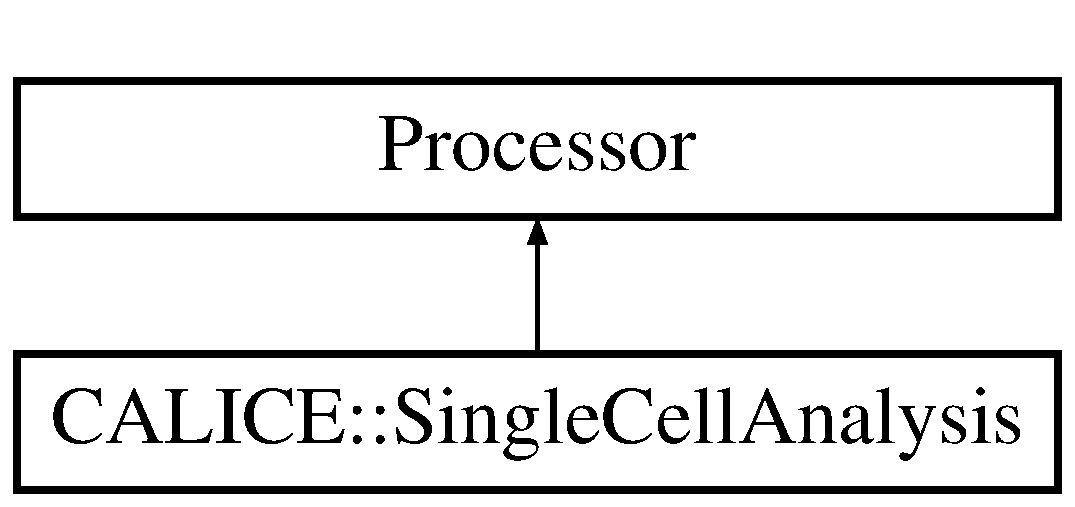
\includegraphics[height=2.000000cm]{classCALICE_1_1SingleCellAnalysis}
\end{center}
\end{figure}
\subsection*{Public Member Functions}
\begin{DoxyCompactItemize}
\item 
virtual Processor $\ast$ {\bfseries new\-Processor} ()\label{classCALICE_1_1SingleCellAnalysis_a3bbce1e034c8128d3ebbe5458500bbd6}

\item 
virtual void {\bfseries init} ()\label{classCALICE_1_1SingleCellAnalysis_a6c48b1978e7397423867c299610f7674}

\item 
virtual void {\bfseries process\-Event} (L\-C\-Event $\ast$evt)\label{classCALICE_1_1SingleCellAnalysis_a047a203f24f82572248c0acae8514257}

\item 
virtual void {\bfseries end} ()\label{classCALICE_1_1SingleCellAnalysis_a7a5e0996495546514a5974d9ea3c5ce9}

\end{DoxyCompactItemize}
\subsection*{Private Member Functions}
\begin{DoxyCompactItemize}
\item 
void {\bfseries update\-Mapping} ()\label{classCALICE_1_1SingleCellAnalysis_a432527a7d5023108adb6028e544786c4}

\end{DoxyCompactItemize}
\subsection*{Private Attributes}
\begin{DoxyCompactItemize}
\item 
unsigned {\bfseries \-\_\-n\-Events}\label{classCALICE_1_1SingleCellAnalysis_a99f44821b039d92c25bf7b13bf4778bc}

\item 
Mapped\-Container\\*
$<$ {\bf Single\-Cell\-Statistics} $>$ $\ast$ {\bfseries \-\_\-cell\-Stat}\label{classCALICE_1_1SingleCellAnalysis_a42a5e7563ad65e0eebf4a0108da517c8}

\item 
Mapped\-Container$<$ T\-H1\-F $>$ $\ast$ {\bfseries \-\_\-cell\-Hist}\label{classCALICE_1_1SingleCellAnalysis_ae4c707658817e2de1b67ac8c348ebf7f}

\item 
std\-::string {\bfseries \-\_\-mapping\-Processor\-Name}\label{classCALICE_1_1SingleCellAnalysis_afc6fc973e6a22a2ca0003076f7c3345b}

\item 
std\-::string {\bfseries \-\_\-calib\-Level}\label{classCALICE_1_1SingleCellAnalysis_a8b30b37473b52f887be5a30806fcd471}

\item 
std\-::string {\bfseries \-\_\-ahcal\-Col\-Name}\label{classCALICE_1_1SingleCellAnalysis_af2763329df8455f7475bdd0d46fdf22f}

\item 
std\-::string {\bfseries \-\_\-txt\-Output\-Name}\label{classCALICE_1_1SingleCellAnalysis_a23feaeb7047a6b87370dd9870385c24c}

\item 
std\-::string {\bfseries \-\_\-root\-Output\-Name}\label{classCALICE_1_1SingleCellAnalysis_a399a21983ff24615e85f186dd59020a1}

\item 
int {\bfseries \-\_\-\-Hist\-\_\-\-E\-Sum\-\_\-xbins}\label{classCALICE_1_1SingleCellAnalysis_ab136d1bac5cce09b328aadcab013468d}

\item 
float {\bfseries \-\_\-\-Hist\-\_\-\-E\-Sum\-\_\-xmin}\label{classCALICE_1_1SingleCellAnalysis_a0d9fe5ae453a208f089f36b7b1ebdc22}

\item 
float {\bfseries \-\_\-\-Hist\-\_\-\-E\-Sum\-\_\-xmax}\label{classCALICE_1_1SingleCellAnalysis_a51a9aa087d66f118aa914f062c9b9fee}

\item 
const Ahc\-Mapper $\ast$ {\bfseries \-\_\-mapper}\label{classCALICE_1_1SingleCellAnalysis_a385a9c5bbbb3d62c2d0741934d064a03}

\item 
unsigned int {\bfseries \-\_\-mapper\-Version}\label{classCALICE_1_1SingleCellAnalysis_a5c6a21d4d86ac54e6039504f97ba741e}

\end{DoxyCompactItemize}


\subsection{Detailed Description}
Processor for analysing cellwise properties like mean signal, R\-M\-S, hit frequency, ... 

The processor creates histograms for each cell summarizing the hit information. In addition, the frequency of hits with respect to the total number of events is determined for each cell.

\begin{DoxyParagraph}{processor parameters}
\begin{TabularC}{3}
\hline
steering file parameter name &description  \\\cline{1-3}
{\bfseries {\itshape  Mapping\-Processor\-Name }}&Name of the Mapping\-Processor instance that provides the geometry of the detector.  \\\cline{1-3}
{\bfseries {\itshape  Hist\-\_\-\-E\-Sum\-\_\-xbins }}&Energy sum histogram\-: number of bins in x-\/axis &\\\cline{1-3}
{\bfseries {\itshape  Hist\-\_\-\-E\-Sum\-\_\-xmin }}&Energy sum histogram\-: lower limit on x-\/axis &\\\cline{1-3}
{\bfseries {\itshape  Hist\-\_\-\-E\-Sum\-\_\-xmax }}&Energy sum histogram\-: upper limit on x-\/axis &\\\cline{1-3}
{\bfseries {\itshape  A\-H\-C\-A\-Lcollection }}&Name of the A\-H\-C\-A\-L Hit collection  \\\cline{1-3}
{\bfseries {\itshape  Output\-File\-\_\-txt }}&Name of the .txt output file  \\\cline{1-3}
{\bfseries {\itshape  Output\-File\-\_\-root }}&Name of the .root output file containing one histogram per cell  \\\cline{1-3}
{\bfseries {\itshape  }}&\\\cline{1-3}
{\bfseries {\itshape  }}&\\\cline{1-3}
{\bfseries {\itshape  }}&\\\cline{1-3}
\end{TabularC}

\end{DoxyParagraph}
\begin{DoxyAuthor}{Author}
{\tt Nils.\-Feege@desy.\-de} 
\end{DoxyAuthor}
\begin{DoxyDate}{Date}
August 2010 
\end{DoxyDate}


Definition at line 54 of file Single\-Cell\-Analysis.\-hh.



The documentation for this class was generated from the following files\-:\begin{DoxyCompactItemize}
\item 
Single\-Cell\-Analysis.\-hh\item 
Single\-Cell\-Analysis.\-cc\end{DoxyCompactItemize}

\section{Single\-Cell\-Statistics Class Reference}
\label{classSingleCellStatistics}\index{Single\-Cell\-Statistics@{Single\-Cell\-Statistics}}
\subsection*{Public Member Functions}
\begin{DoxyCompactItemize}
\item 
{\bf Single\-Cell\-Statistics} $\ast$ {\bfseries add\-\_\-hit} (double E\-Sum)\label{classSingleCellStatistics_a6a56d2dc810b72a4e5b4ded0422f8199}

\item 
int {\bfseries get\-\_\-n\-\_\-hits} ()\label{classSingleCellStatistics_aba90a0ea0bee6c636e3b369bd4338b06}

\item 
double {\bfseries get\-\_\-energy\-\_\-sum} ()\label{classSingleCellStatistics_aff5d2589b7c310995b2866e22f1def7e}

\item 
double {\bfseries get\-\_\-energy\-\_\-mean} ()\label{classSingleCellStatistics_ac921eb395cba1336b676ada1c9d15772}

\item 
double {\bfseries get\-\_\-energy\-\_\-rms} ()\label{classSingleCellStatistics_a7a72f85e2a683197655dc1bc1bea68d2}

\item 
double {\bfseries get\-\_\-hit\-\_\-energy\-\_\-max} ()\label{classSingleCellStatistics_aba089759ba105f50be7a4f21902f318f}

\end{DoxyCompactItemize}
\subsection*{Private Attributes}
\begin{DoxyCompactItemize}
\item 
int {\bfseries \-\_\-n\-\_\-hits}\label{classSingleCellStatistics_a518a9edb2a31a08301e08adaf9a8b41a}

\item 
double {\bfseries \-\_\-energy\-\_\-sum}\label{classSingleCellStatistics_a3a38fb073934aef88f90bf0a2257f235}

\item 
double {\bfseries \-\_\-energy\-\_\-squared\-\_\-sum}\label{classSingleCellStatistics_aeb92f74c92dae3392d08c160a5dbe252}

\item 
double {\bfseries \-\_\-hit\-\_\-energy\-\_\-max}\label{classSingleCellStatistics_a3bd8c04ddf2ce3aa47196220480c3a5a}

\end{DoxyCompactItemize}


\subsection{Detailed Description}


Definition at line 10 of file Single\-Cell\-Statistics.\-hh.



The documentation for this class was generated from the following file\-:\begin{DoxyCompactItemize}
\item 
Single\-Cell\-Statistics.\-hh\end{DoxyCompactItemize}

%--- End generated contents ---

% Index
\newpage
\phantomsection
\addcontentsline{toc}{part}{Index}
\printindex

\end{document}
